% ----------------------------------
% 1-Preambulo.
% ----------------------------------
\documentclass[12pt,a4paper]{article}
\usepackage[spanish,es-tabla]{babel}
\usepackage[T1]{fontenc}
\usepackage{textcomp}
\usepackage{lmodern}
\usepackage[utf8]{inputenc}
\usepackage{graphicx}
\usepackage[procnames]{listings} 	%Para escribir códigos.
\usepackage[none]{hyphenat}         %Para no recortar las palabras con guión.
% OJO: se agregaron procnames para usarlos en Python (VER).

\usepackage[bottom]{footmisc} 	 	%Para poner las footnote al final de cada página.
\usepackage[hidelinks]{hyperref} 	%Para que el indice pueda ser linkeado.
\usepackage{amssymb}			 	%Para ecuaciones matemáticas.
\usepackage{amsmath}				%Para matrices.
\usepackage{mathtools}
\usepackage{amsfonts} 
\usepackage{verbatim}				%Para usar comentarios.
\parskip 0.1in 						%Distancia parrafos.

%Biliografías:
%\usepackage[style=authoryear]{biblatex}
%\addbibresource{bibliografias.bib}

\usepackage{float} 							%Para que no se muevan las imágenes de lugar.

\usepackage[
  separate-uncertainty = true,
  multi-part-units = repeat
]{siunitx} 									%Para el \SI del +- .

\usepackage[margin=0.984252in]{geometry} 	%Para los márgenes.
\usepackage{subcaption}
\usepackage{appendix} 						%Para los anexos.

% ----------------------------------
% 1.1-Anexos.
% ----------------------------------

%begin anexos
\makeatletter
\def\@seccntformat#1{\@ifundefined{#1@cntformat}  	%"\@seccntformat" es un comando auxiliar.
   {\csname the#1\endcsname\quad}  					%Default.
   {\csname #1@cntformat\endcsname}					%Enable individual control.
}

\let\oldappendix\appendix 							%Guarda la definicion vigente de \appendix
\renewcommand\appendix{%
    \oldappendix
    \newcommand{\section@cntformat}{\appendixname~\thesection\quad}
}
\makeatother
%\renewcommand{\appendixname}{Anexos}
%\renewcommand{\appendixtocname}{Anexos}
%\renewcommand{\appendixpagename}{Anexos}
%end anexos

% ----------------------------------
% 1.2-Para código Python. 
% ----------------------------------
\usepackage{color}
\definecolor{keywords}{RGB}{255,0,90}
\definecolor{comments}{RGB}{0,0,113}
\definecolor{red}{RGB}{160,0,0}
\definecolor{green}{RGB}{0,150,0}
 
\lstset{language=Python, 
        basicstyle=\ttfamily\small, 
        keywordstyle=\color{keywords},
        commentstyle=\color{comments},
        stringstyle=\color{red},
        showstringspaces=false,
        identifierstyle=\color{green},
        procnamekeys={def,class}}

% ----------------------------------
% 1.3-Índice. 
% ----------------------------------

\setcounter{secnumdepth}{3} 		%Para que ponga 1.1.1.1.
\setcounter{tocdepth}{4} 			%Para que añadir las secciones en el Índice.
\usepackage{chngcntr}				%Para que el número de las figuras esten acordes a la sección.
\counterwithin{figure}{section}

\author{
	\textbf{Ingeniería en Informática}\\
	Departamento de Tecnología y Administración\\
	\\~\\
	Tesista\\
	\textbf{Calonge, Federico Matias}\\
	calongefederico@gmail.com
 	\\~\\
 	Director\\ 
 	\textbf{Ing. D'Angiolo, Federico Gabriel}\\
 	fdangiolo@undav.edu.ar
 	\\~\\
 	Co-Director\\ 
 	\textbf{Dr. Asteasuain, Fernando}\\
 	fasteasuain@undav.edu.ar
}

\title{
  Tesis \\
  \large Automatización de lectura de Curriculum Vitae  \\
    para selección de personal en el sector IT}
\date{Diciembre 2022}
    
%Para modificar los parrafos y para que se pueda poner subsections:
\makeatletter
\renewcommand\paragraph{\@startsection{paragraph}{4}{\z@}
            {-2.5ex\@plus -1ex \@minus -.25ex}
            {1.25ex \@plus .25ex}
            {\normalfont\normalsize\bfseries}}
\makeatother
\setcounter{secnumdepth}{4} 	%How many sectioning levels to assign numbers to.
\setcounter{tocdepth}{4}    	%How many sectioning levels to show in ToC.
% ----------------------------------
% 2-Documento
% ----------------------------------

\begin{document}

\begin{sloppypar}
\begin{figure}
  \centering
  
\includegraphics[width=0.2\textwidth]{images/undav-logo.png} 	%Incluyendo logo de la Undav.
  \label{fig:undav-logo}
\end{figure}
\maketitle       		%Para generar el título definido arriba.

\cleardoublepage    %Nueva página

\begin{center}
    \Large
    \vspace{0.9cm}
    \textbf{Resumen}
    
\end{center}

En la Tesis de Ingeniería en Informática que se presenta se diseña un \textit{sistema de lectura automática de Curriculum Vitae} accesible vía Web. La finalidad del mismo es ayudar al reclutador laboral a elegir a los mejores candidatos para los puestos laborales de IT que tenga disponible. Esta elección se realiza mediante el uso de algoritmos de \textit{machine learning} y basándose, principalmente, en una medición de similitud entre textos: Curriculum Vitae de los candidatos por un lado, y descripciones de los puestos laborales de IT por el otro.
El sistema esta desarrollado utilizando el lenguaje de programación Python, permitiendo verificar la teoría desarrollada.

\begin{center}
    \Large
    \vspace{0.9cm}
    \textbf{Abstract}
\end{center}

This Computer Engineering Thesis introduces an \textit{automatic Curriculum Vitae reading system} accesible via the Web. The purpose of it is to help the job recruiter to choose the best candidates for the available IT job positions. This choice is made through the use of \textit{machine learning} algorithms and based mainly on a measurement of similarity between texts: Curriculum Vitae of the candidates on the one hand, and IT job descriptions on the other hand.
The system is developed using the Python programming language allowing to verify the developed theory.

\cleardoublepage    %Nueva página

\tableofcontents 	%Para insertar el índice general.

\cleardoublepage    %Nueva página

\section{Introducción.}\label{Intro}
Los procesos de \textit{reclutamiento y selección laboral} se han vuelto cruciales para el manejo de recursos humanos en el mundo moderno. Con las transformaciones digitales de las empresas y del mercado laboral en general, identificar los perfiles más acordes a las necesidades de la empresa se convirtió en uno de los retos más ambiciosos de Recursos Humanos, en especial cuando hablamos del \textit{Sector IT}, donde año tras año se van generando nuevos puestos de trabajo y estos mismos van creciendo en demanda. Este crecimiento de la demanda en distintos puestos del Sector IT lo podemos evidenciar, a modo de resumen, en la Figura \ref{fig:Increasing_Jobs}.

En estos últimos años se implementaron una gran cantidad de herramientas de Software que utilizan algoritmos inteligentes y que permiten automatizar y gestionar información de los candidatos de una manera mucho más intuitiva\cite{trabajos_relacionados_1,trabajos_relacionados_2,trabajos_relacionados_3,trabajos_relacionados_4,
trabajos_relacionados_5,trabajos_relacionados_6,trabajos_relacionados_7,trabajos_relacionados_8,
trabajos_relacionados_9,trabajos_relacionados_10, trabajos_relacionados_11, trabajos_relacionados_12, trabajos_relacionados_13, trabajos_relacionados_14, trabajos_relacionados_15}. La \textit{automatización} se transformó en un factor clave e indispensable para que el reclutador pueda conseguir a los candidatos más relevantes para los puestos que ofrece la empresa en un tiempo muy corto.
Se espera que para el año 2025 muchas tareas realizadas actualmente por humanos, sean automatizadas por máquinas: esto lo podemos evidenciar en la Figura \ref{fig:Automatizacion}.

\begin{figure}[H]    %[H] es para que se ubique justo debajo del texto anterior. 
  \centering
  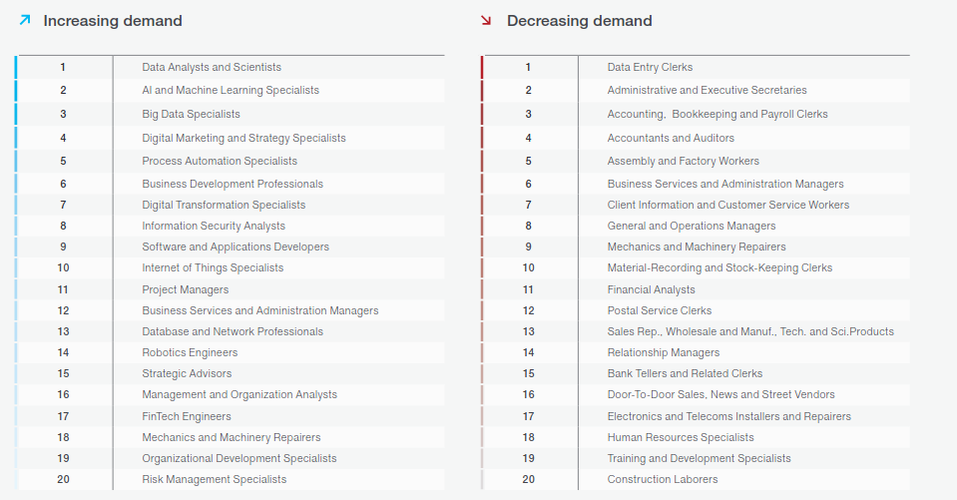
\includegraphics[width=1\textwidth]{images/Increasing_Jobs.png} 	%Incluyendo imagen Flow Core.
  \caption{Top 20 demanda de roles laborales en aumento y disminución para el año 2020, por participación de las empresas encuestadas por el \textit{Foro Económico Mundial}\cite{jobs_future}.}  
  \label{fig:Increasing_Jobs}
\end{figure}

\begin{figure}[H]    %[H] es para que se ubique justo debajo del texto anterior. 
  \centering
  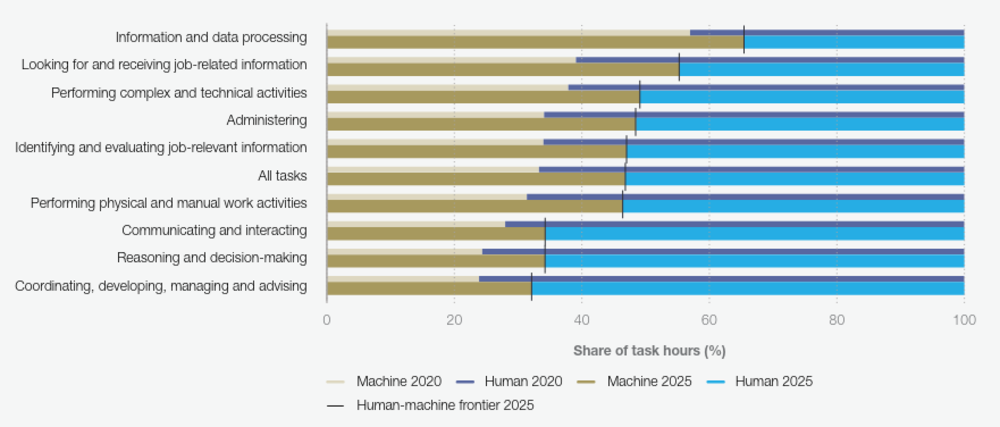
\includegraphics[width=1\textwidth]{images/Automatizacion.png} 	%Incluyendo imagen Flow Core.
  \caption{Porcentaje de tareas realizadas por humanos frente a máquinas, 2020 y 2025 (previsto),
por participación de las empresas encuestadas por el \textit{Foro Económico Mundial}\cite{jobs_future}.}  
  \label{fig:Automatizacion}
\end{figure}

El tema de este Proyecto de Tesis será desarrollar un \textit{sistema de lectura automática de Curriculum Vitae} accesible vía Web. La finalidad del mismo es ayudar al reclutador laboral a elegir a los mejores candidatos para los puestos laborales de IT que tenga disponible. Esta elección se realiza mediante el uso de algoritmos de machine learning y basándose, principalmente, en una medición de similitud entre textos: Curriculum Vitae de los candidatos por un lado, y descripciones de los puestos laborales de IT por el otro.

La medición de similitudes entre documentos de texto (text similarity measurement) es uno de los problemas más cruciales del \textit{Procesamiento del Lenguaje Natural (NLP)}. Encontrar similitudes entre documentos se utiliza en varios dominios de NLP, tales como en sistemas de recomendación, de information retrieval (IR), de análisis de sentimientos, etc.\cite{Similarity_calculation}

Para que las máquinas puedan describir esta similitud entre documentos, se necesita definir una forma de medir matemáticamente la similitud, la cual debe ser comparable para que la máquina pueda identificar qué documentos son más (o menos) similares. Previamente a esto necesitamos representar el texto de los documentos en una forma cuantificable (que suele ser en forma vectorial), de modo que podamos realizar los posteriores cálculos de similitud sobre él. Una distancia pequeña entre los vectores significa un alto nivel de similitud, mientras que grandes distancias significan un bajo nivel de similitud\cite{Similarity_calculation}.

Por lo tanto, resumidamente los pasos necesarios para poder medir similitudes entre documentos son\cite{Similarity_calculation}:
\begin{enumerate}
\item Convertir cada uno de los documentos de texto en un objeto matemático (vector).
\item Definir y emplear una métrica de distancia que será utilizada como nuestra medida de similitud entre los textos.
\end{enumerate}

\cleardoublepage    %Nueva página

En el sistema desarrollado, una vez obtenidas estas mediciones de similitud entre los Curriculum Vitae de los candidatos y las descripciones de los puestos laborales de IT mediante distintos algoritmos y técnicas de machine learning, estos valores se utilizarán para alimentar y generar \textit{un modelo de clasificación}, el cual nos servirá para lograr, en base a los valores de similitud de nuevos candidatos, clasificar qué tan similares son dichos candidatos con respecto a la descripción de un puesto de IT: similitud escasa, similitud media, similitud alta, similitud muy alta.\\

\subsection{Algoritmos y técnicas utilizadas.}

A continuación nombraremos resumidamente los algoritmos y técnicas de machine learning utilizadas para el desarrollo del \textit{sistema de lectura automática de Curriculum Vitae}. 

Como se mencionó en \textit{\nameref{Intro}}, el primer paso para lograr nuestra medición de similitudes entre documentos consiste en convertir los documentos en vectores: para esto se utilizaron las técnicas de vectorización \textbf{TF-IDF} y \textbf{Word embeddings}.

Para el segundo paso, definir y emplear métricas de distancia, se decidió emplear una combinación de las técnicas \textbf{Cosine Similarity} y \textbf{Word Mover’s Distance (WMD)}. En la sección \textit{\nameref{cos_y_wmd}} se detallan las razones por las cuales se decidieron elegir estos métodos; las cuales están justificadas en base al análisis realizado en la sección \textit{\nameref{Tecnicas_Simil_textos}}, en el cual se detallan las numerosas técnicas existentes para obtener similitudes entre textos.

Como tercer y último paso, una vez obtenidas estas mediciones de similitud entre los Curriculum Vitae de los candidatos y las descripciones de los puestos laborales de IT, estos valores se utilizaron para alimentar un \textbf{algoritmo de clustering K-means} que a su vez, con sus datos de salida (4 clusters), alimentan a un \textbf{modelo de clasificación K-Nearest Neighbor (KNN)}.

Finalmente, con este modelo KNN logramos, en base a los valores de similitud de nuevos candidatos, clasificar qué tan similares son dichos candidatos con respecto a la descripción de un puesto de IT.

Estos algoritmos, técnicas y modelos utilizados serán detallados en las secciones posteriores, tanto teóricamente como en su implementación. 

\cleardoublepage    %Nueva página

\subsection{Objetivos del Proyecto.}

\subsubsection{Objetivo general.}

El objetivo de este Proyecto de Tesis es lograr un desarrollo, tanto teórico como práctico, de un \textit{sistema de lectura automática de Curriculum Vitae} accesible vía Web. La finalidad del mismo es ayudar al reclutador laboral a elegir a los mejores candidatos para los puestos laborales de IT que tenga disponible. Esta elección se realiza mediante el uso de algoritmos de machine learning y basándose, principalmente, en una medición de similitud entre textos:  
\begin{itemize}
\item los Curriculum Vitae de los candidatos por un lado, 
\item descripciones de los puestos laborales de IT por el otro.
\end{itemize} 

\subsubsection{Objetivos específicos.}\label{Obj_especif}
Los objetivos específicos de este Proyecto de Tesis son:
\begin{itemize}
\item Describir el estado del arte actual de los Sistemas de lectura y análisis de Curriculum Vitae en las fases de reclutamiento y selección laboral. 
\item Implementar un Sistema de lectura automática de Curriculum Vitae basado en la comparación y medición de similitudes entre textos, para finalmente obtener una visualización de los mejores candidatos para un puesto laboral de IT determinado.  
\item Aprender los conceptos y técnicas principales utilizadas dentro del procesamiento de lenguaje natural (NLP) aplicando técnicas de preprocesamiento y limpieza de textos.
\item Implementar diferentes técnicas para medir similitudes entre los textos (Cosine Similarity y  Word Mover's Distance -WMD-) y diferentes técnicas de vectorización (TF-IDF y Word embeddings), analizando su funcionamiento tanto teórica como matemáticamente, ventajas y desventajas.
\item Conocer, implementar e integrar el algoritmo de clustering K-means junto al algoritmo de clasificación KNN para obtener un modelo de clasificación de candidatos en base a las medidas de similitud entre los textos.
\item Evaluar los Frameworks disponibles para tener una UI \footnote{La interfaz de usuario o user inteface (UI) de una página web refiere a todo aquello tangible con lo que los usuarios interactúan de forma directa en la misma.} accesible vía web e integrar el mismo al Sistema.
\item Almacenar datos de candidatos, reclutadores y puestos laborales en una base de datos.
\end{itemize} 

\cleardoublepage    %Nueva página

\subsection{Alcance del Proyecto.}
El alcance de esta Tesis de Grado de Ingeniería incluye el desarrollo de conceptos de análisis de datos y machine learning, procesamiento de lenguaje natural, técnicas de preprocesamiento y limpieza de los datos, técnicas de vectorización y técnicas para medir la similitud entre textos, algoritmos de clasificación y clustering, integración con frameworks, visualización de datos, y gestión de Base de Datos, de acuerdo a lo enunciado en los \textit{\nameref{Obj_especif}}.

\subsection{Organización.}\label{organizacion}
Este Proyecto de Tesis fue organizado para trabajarlo en tres secciones:

\begin{enumerate}
\item Análisis e investigación inicial. 

Esta sección abarca principalmente la parte teórica del trabajo, haciendo hincapié en el análisis e investigación de:
\begin{itemize}
	\item El estado del arte (actual y pasado) de los sistemas de lectura y análisis de Curriculum Vitae.
	\item Técnicas usadas para el procesamiento del lenguaje natural (NLP).
	\item Técnicas para medir similitudes entre textos: Cosine Similarity y WMD.
	\item Técnicas de vectorización: TF-IDF y Word embeddings.
	\item Algoritmos de machine mearning para tareas de clasificación (KNN) y clustering (K-means).
\end{itemize} 

Esta primera sección abarca los capítulos \textit{\nameref{2.ReclutamientolaboralenIT}}, \textit{\nameref{3.AlgoritmosdeMachineLearning}} y \textit{\nameref{4.NaturalLanguageProcessing}} de este Informe de Tesis. \\

\item Implementación de distintas técnicas y algoritmos para la obtención del modelo de clasificación KNN. 

Esta sección hace referencia a la aplicación práctica dentro del marco teórico desarrollado en la primera sección, mediante la realización de una serie de análisis en documentos de Jupyter Notebook\footnote{Aplicación cliente-servidor que permite crear documentos web en formato JSON que siguen un esquema versionado y una lista ordenada de celdas de entrada y de salida. Estas celdas albergan, entre otras cosas, código, texto (en formato Markdown), fórmulas y ecuaciones matemáticas. Estos documentos que se generan funcionan en cualquier navegador estándar.} utilizando Python \footnote{Lenguaje de programación interpretado y multiplataforma de código abierto, popularizado en los últimos años por su facilidad para trabajar con inteligencia artificial, big data, machine learning y data science, entre muchos otros campos en auge.}, para la obtención final de nuestro modelo de clasificación KNN capaz de clasificar, en base a los valores de similitud de nuevos candidatos, qué tan similares son dichos candidatos con respecto a la descripción de un puesto de IT: similitud escasa, similitud media, similitud alta, similitud muy alta. 

\cleardoublepage    %Nueva página

Los items que abarca esta sección son:

\begin{itemize}
	\item Obtención de sets de datos: curriculums vitae y descripciones laborales. 
	\item Preprocesamiento de los textos.
	\item Comparación entre textos y obtención de similitudes entre los mismos mediante el uso de las técnicas para medir distancias y obtener dichas similitudes (WMD y Cosine Similarity) y las técnicas de vectorización (TF-IDF y Word embeddings).
	\item Obtención del modelo de clasificación KNN utilizando como datos de entrada los clusters devueltos por el algoritmo K-means obtenidos en base a las mediciones de similitud previamente realizadas.
	\item Análisis y primeras visualizaciones de los resultados.
\end{itemize} 
 
Esta sección abarca el capítulo \textit{\nameref{5.Implementacion}} (desde \textit{\nameref{5.1.Obtenciondelmodelopredictivo}} hasta \textit{\nameref{5.4.Predicciondenuevasmuestrasyresultadosobtenidos}}) de este Informe de Tesis. \\

\item Integración al sistema web.

Esta última sección hace referencia a la reutilización de las funciones que contienen la lógica de los distintos algoritmos utilizados junto con el modelo de clasificación KNN obtenidos previamente en la sección 2, para integrar todo este conjunto en el sistema web que, a su vez, esta integrado a una base de datos relacional. De esta manera, el sistema cuenta con una interfaz gráfica que permite al reclutador cargar los Curriculums Vitae de los candidatos y los puestos que tenga disponible, y principalmente obtener un listado con los candidatos más similes a un puesto determinado, ordenados de mayor a menor de acuerdo a esta \textit{similitud}. Dicha \textit{similitud} representa el resultado obtenido de la clasificación por nuestro modelo KNN.

Los items principales de esta sección son:
\begin{itemize}
	\item Definición de los usuarios que accederán al sistema.
	\item Definición de los datos que se almacenarán.
	\item Integración de frameworks y bases de datos.  
	\item Modelado, filtrado y visualización de los datos.
	\item Reutilización e integración al sistema de los algoritmos y del modelo KNN utilizados en la fase previa.	
	\item Evaluación del funcionamiento de todo el Sistema integrado.
\end{itemize} 

Esta última sección abarca el capítulo \textit{\nameref{5.Implementacion}} (desde \textit{\nameref{5.5.IntegracionalSistemaWeb}} hasta el final del capítulo) de este Informe de Tesis.
\end{enumerate}

\cleardoublepage    %Nueva página

\section{Reclutamiento y selección laboral.}\label{2.ReclutamientolaboralenIT}

En este capítulo se va a realizar una introducción a los procesos de reclutamiento y selección laboral, sus diferencias y diferentes tareas involucradas. Por último, se llevará a cabo un análisis del Estado de Arte actual de los sistemas de cribado (o más conocidos como sistemas de \textit{screening}) y se detallará el enfoque utilizado para este Proyecto.

\subsection{Introducción.}

Los procesos de \textit{reclutamiento y selección laboral} se han vuelto cruciales para el manejo de recursos humanos en el mundo moderno. Con las transformaciones digitales de las empresas y del mercado laboral en general, identificar los perfiles más acordes a las necesidades de la empresa se convirtió en uno de los retos más ambiciosos de Recursos Humanos, en especial cuando hablamos del \textit{Sector IT}, donde año tras año se van generando nuevos puestos de trabajo y estos mismos van creciendo en demanda. 

Los \textit{reclutadores}, dentro de un departamento de recursos humanos, son los encargados de llevar a cabo los procesos de \textit{reclutamiento} y \textit{selección} laboral. Uno de sus objetivos principales es buscar talento humano para cubrir los puestos de trabajo vacantes que tenga la empresa.

\subsection{Reclutamiento vs selección.}\label{SeleccionYReclutamiento}

El \textbf{reclutamiento} es el proceso de atracción, búsqueda, recolección e identificación de candidatos que encajan con la oferta de trabajo y, en definitiva, con la empresa. Como mencionan Anwar y Abdullah, \textit{``el reclutamiento es el proceso de descubrir y capturar candidatos calificados o apropiados para ocupar el puesto vacante''}\cite{seleccion_reclutamiento_2}.

El objetivo del reclutamiento es \textit{atraer}, \textit{buscar} e \textit{identificar} a los candidatos más adecuados y mejor calificados para el puesto disponible, según las necesidades de la empresa. 

El proceso de reclutamiento incluye las siguientes actividades\cite{seleccion_reclutamiento_2}:
\begin{itemize}
\item Identificación de las necesidades del puesto a cubrir. 
\item Análisis de la descripción y especificaciones del puesto.
\item Identificación de posibles fuentes de candidatos cualificados para el puesto.
\item Publicacion del puesto vacante en dichas fuentes.
\item Atracción de candidatos para aplicar al puesto.
\item Manejo apropiado en las respuestas y en los escrutinios a las postulaciones.
\end{itemize}

\cleardoublepage    %Nueva página

En cambio, la \textbf{selección} es un proceso posterior al reclutamiento, donde se evalua más detalladamente y se entrevista a los candidatos para el trabajo en particular. Como mencionan Rahman y Abdullah, \textit{``la selección es un proceso de evaluar y entrevistar a los candidatos para un trabajo en particular y seleccionar a la persona adecuada para el puesto correcto''}\cite{seleccion_reclutamiento_2}.

El objetivo de la selección es \textit{elegir} y \textit{hacer efectiva la contratación} del candidato más adecuado y mejor calificado para el puesto disponible, según las necesidades de la empresa. Este procedimiento particiona a los candidatos en dos secciones: a los que se les ofrecerán el trabajo, y a los que se descartarán.

El proceso de selección incluye las siguientes actividades\cite{seleccion_reclutamiento_2}: 
\begin{itemize}
\item Recepción de la aplicación al puesto.
\item Cribado o Screening de los candidatos, lo que permite avanzar con los candidatos adecuados y descartar a los no adecuados para el puesto.
\item Entrevistas a los candidatos.
\item Manejo de tests a los candidatos, tales como tests médicos o psicológicos. 
\item Manejo de exámenes a los candidatos, tales como exámenes técnicos, de aptitud, inteligencia, performance, etc.
\item Evaluación de las referencias de los candidatos.
\item Decisión final acerca de la contratación o no contratación del candidato.
\end{itemize}

Como conclusión, podemos decir que en la fase de \textbf{reclutamiento} se trata de encontrar muchos candidatos que cumplan con los requisitos de la oferta; mientras que en la etapa de \textbf{selección} se debe elegir al mejor candidato para las necesidades de la empresa. 

\cleardoublepage    %Nueva página

\subsection{Evolución de los procesos de reclutamiento y selección laboral.}
Los procesos de reclutamiento y selección laboral fueron evolucionando a lo largo del tiempo\cite{trabajos_relacionados_10}:

En los modelos de reclutamiento y selección de \textbf{primera generación}, las empresas anunciaban sus vacantes de puestos laborales en diarios, revistas, radio y en televisión. Los candidatos enviaban sus currículums por correo postal y los mismos se clasificaban manualmente: algo muy tedioso y que llevaba mucho tiempo en realizar. Una vez \\ preseleccionados los candidatos, los reclutadores llamaban a los mismos para realizar las rondas de entrevistas. 

Luego pasamos a la \textbf{segunda generación}. En esta época las empresas comenzaron a crecer y también lo hicieron las necesidades de reclutamiento y selección. Las empresas empezaron a subcontratar sus procesos de reclutamiento y selección, naciendo de esta manera las consultoras o agencias de contratación. Estas consultoras requerían que los candidatos cargaran sus currículums en sus sitios web en formatos particulares. Luego, las consultoras revisaban los datos de los candidatos y preseleccionaban a los mismos para la empresa. El gran inconveniente de este proceso fue que habían numerosas consultoras y cada una tenía su propia y única forma de selección, no era un proceso uniforme.

Para intentar superar los problemas anteriores, se llegó a una \textbf{tercera generación}, en la que estamos actualmente. En esta generación se crearon, y siguen creándose, una gran cantidad de herramientas de Software que utilizan algoritmos inteligentes y permiten automatizar y gestionar información de los candidatos de una manera mucho más intuitiva. Estos sistemas ayudan a los reclutadores dentro de las empresas y consultoras a analizar la información de cualquier Curriculum Vitae y clasificarlos o listarlos en función de los puestos disponibles. De esta manera, cuando el reclutador publica una oferta de trabajo, estos sistemas clasifican o listan a los currículums basándose en distintas métricas (por ejemplo palabras clave) mostrando así los candidatos más relevantes para la empresa o consultora.

\cleardoublepage    %Nueva página

\subsection{Cribado o screening.}  

Como vimos anteriormente en \textit{\nameref{SeleccionYReclutamiento}}, el screening (o tambien conocido como cribado) es una etapa del proceso de selección. 
En esta etapa los reclutadores revisan los Currículums Vitae que fueron recibiendo por parte de los candidatos, y \\ preseleccionan a los que mejor se adapten a los requisitos de la oferta de empleo de la empresa. Este proceso es muy importante dentro del proceso de selección, ya que permite valorar en ese momento si el candidato es apto para continuar en el proceso de selección o, en caso contrario, si el mismo se descarta por no considerarlo adecuado para el puesto.

\subsubsection{Screening manual vs screening automatizado}  

Si el proceso de screening sigue el modelo tradicional y se realiza manualmente, es un proceso muy tedioso y que lleva mucho tiempo por parte del reclutador, el cual tiene que evaluar una gran cantidad de Curriculums Vitae. Existe un estudio\cite{estudio_eye_tracking} relizado en 2018 por Ladders Inc., empresa lider en sitios de carrera, donde se estudió cuánto tiempo en promedio tarda un reclutador en dar una primera vista rápida a un Curriculum Vitae de un candidato. Se descubrió que este tiempo es, en promedio, de 7.4 segundos. Este es el tiempo en el que el reclutador decide inicialmente si el candidato sigue (o no) con el proceso de selección.

Sin embargo, este tiempo es engañoso: ya que este estudio fue realizado con la aplicación de muchos Curriculums vitae que no cumplian con los criterios mínimos para calificar a los puestos; es por esto que los reclutadores realizaban una primer vista rápida y los descartaban (o no) a los pocos segundos. Si las aplicaciones provenieran de Curriculums Vitae que cumplan con los requisitos mínimos del puesto, este tiempo de observación sería mucho mayor, ya que el reclutador examinaría con mayor detalle los curriculums.

Adicionalmente, este estudio tampoco tiene en cuenta el tiempo consumido por el reclutador al comparar el Curriculum Vitae del candidato con la descripción o requisitos del puesto laboral, por lo que el tiempo en realizar un screening manual se incrementaría significativamente.

Otra de las desventajas al considerar el screening como un proceso manual, es que muchos son los factores que pueden influir al reclutador en el momento de tomar la decisión de descarte o selección del candidato, ya sea cansancio por el volumen de los curriculums ya revisados, la estructura, elementos discriminatorios o información incompleta dentro de los mismos, etc. Es por esto que las probabilidades de descartar prematuramente a un candidato válido son muy altas.

Frente a estas desventajas del modelo tradicional y poco eficiente del screening manual existe una solución: la \textit{automatización}. Actualmente existen sistemas automatizados y basados en Inteligencia Artificial que permiten realizar el screening de un volumen importante de curriculums en unos pocos segundos (Ver \textit{\nameref{Estado_del_arte}}). De esta manera, el proceso de screening no estaría afectado a factores externos que puedan influir en la decisión del reclutador, y además la herramienta sería capaz de entregar un listado justificado de los mejores candidatos para la siguiente fase del proceso en un tiempo relativamente corto.

\cleardoublepage    %Nueva página

Uno de los beneficios potenciales de utilizar sistemas automatizados e inteligentes en los procesos de screening es el acortamiento de los ciclos de contratación, lo que hace que la organización responda mejor a los solicitantes y sea más capaz de competir con otras organizaciones por los mejores candidatos\cite{seleccion_reclutamiento_1}.  

Muchos gerentes de recursos humanos depositan sus esperanzas en la tecnología y las herramientas automatizadas e inteligentes: desde el aumento de la eficiencia y la reducción de costos hasta el aumento de las aplicaciones de candidatos y la estandarización de todos sus sistemas de selección\cite{seleccion_reclutamiento_1}.

\subsection{Sistemas de screening: Estado del arte.}\label{Estado_del_arte}

Tal como mencionamos en la sección anterior, un sistema de screening automatizado e inteligente nos permite entregar al reclutador una shortlist con los candidatos que mejor se adaptan a los requisitos de la oferta de empleo de la empresa. De esta manera, al realizar dicha preselección de candidatos, el reclutador podrá seguir con las etapas posteriores de selección o podrá realizar otro screening manual para descartar a otros candidatos.

A continuación detallaremos una serie de trabajos de relevancia (tanto de implementación como de investigación) donde se utilizaron distintos enfoques para desarrollar o sugerir un desarrollo de un sistema de screening de candidatos.

En \cite{trabajos_relacionados_1} utilizaron el \textit{algoritmo KNN} para clasificar los curriculums de los candidatos en diferentes categorías, y luego utilizaron la métrica de similitud \textit{Cosine Similarity} para averiguar qué tan cerca está el curriculum del candidato con respecto a la descripción de los puestos, y realizar un ranking acorde a estos resultados.

En \cite{trabajos_relacionados_2} utilizaron una herramienta inteligente llamada \textit{EXPERT mapping-based candidate screening} que utiliza  \textit{ontology mapping}\footnote{La \textit{ontología (ontology)} permite la especificación explícita de un dominio de discurso, que permite acceder y razonar sobre el conocimiento de un agente. Las ontologías elevan el nivel de especificación del conocimiento, incorporando semántica a los datos.
El \textit{mapeo de ontologías (ontology mapping)} es el proceso mediante el cual dos ontologías se relacionan semánticamente a nivel conceptual y las instancias de ontología de origen se transforman en entidades de ontología de destino de acuerdo con esas relaciones semánticas.\cite{ontology_mapping} } para crear un sistema automatizado para el screening inteligente de candidatos. 

En \cite{trabajos_relacionados_3} y \cite{trabajos_relacionados_4} también se utilizan sistemas basados en \textit{ontologías} para extraer datos de curriculums y realizar macheos con los puestos disponibles.

En \cite{trabajos_relacionados_5} sugieren un método de matching basado en un \textit{modelo probabilístico} para ser utilizado en la selección y recomendación de candidatos. 

En \cite{trabajos_relacionados_6} se propuso un aistema automatizado de screening de currículums que usa \textit{Vector Space Model}\footnote{Modelo algebraico para representar documentos de textos en lenguaje natural de una manera formal mediante el uso de vectores de identificadores. Es utilizado para la recuperación, filtrado, indexado y cálculo de relevancia de información.} para machear cada curriculum con la descripción del puesto correspondiente y \textit{Cosine Similarity} como medida de similitud.

\cleardoublepage    %Nueva página

En \cite{trabajos_relacionados_7} y \cite{trabajos_relacionados_8} se propuso un sistema para el screening de candidatos, para el cual se utiliza \textit{Cosine Similarity}, \textit{KNN} y un \textit{sistema de recomendación basado en contenido (Content Based Filtering, CBF)} para buscar los curriculums más cercanos a la descripción del puesto.

En \cite{trabajos_relacionados_9} se propuso un sistema para el ordenamiento y clasificación de currículums utilizando el concepto de inteligencia artificial (sin especificar qué algoritmos o técnicas específicas se deberían usar). Lo que se propuso fue un esquema de trabajo para luego seguir con la implementación del sistema; el cual permitiría clasificar a todos los currículums de acuerdo con los requisitos de la empresa y los enviaría a Recursos Humanos para su posterior consideración.

En \cite{trabajos_relacionados_10} se diseñó un sistema que ayuda a los reclutadores a seleccionar los curriculums basados en la descripción del trabajo. Ayuda en un proceso de contratación fácil y eficiente al extraer los requisitos automáticamente. Este sistema utiliza un \textit{modelo NER (Named entity recognition)} \footnote{Subtarea de \textit{information extraction (IE)} que permite buscar y categorizar entidades específicas en un cuerpo o cuerpos de textos.}.

En \cite{trabajos_relacionados_11} y \cite{trabajos_relacionados_12} se implementan sistemas basados en \textit{semantic anotation}\footnote{Proceso de etiquetado de documentos con conceptos relevantes. Los documentos se enriquecen con metadatos que permiten vincular el contenido a los conceptos, descritos en un gráfico de conocimiento. Esto hace que el contenido no estructurado sea más fácil de encontrar, interpretar y reutilizar.} y \textit{ontologías}, permitiendo realizar macheos entre las ofertas de trabajo y los curriculums de los candidatos.

En \cite{trabajos_relacionados_13} se utiliza \textit{relevance feedback}\footnote{Característica de algunos sistemas de \textit{information retrieval (IR)}. La idea de relevance feedback es tomar los resultados que se devuelven inicialmente de una consulta/query determinada, recopilar los comentarios de los usuarios y usar información para evaluar si esos resultados son relevantes o no para realizar una nueva consulta/query.} para la implementación de un sistemas que intenta encontrar a los mejores candidatos para las distintas ofertas de trabajo.

\textit{Paul Resnick} y \textit{Hal R. Varian} fueron pioneros en los \textit{sistemas de recomendación}\footnote{Un \textit{sistema de recomendación} es una subclase de los sistemas de \textit{Information filtering (IF)} que busca predecir la calificación o la preferencia que un usuario le puede dar a un artículo. En palabras simples, es un algoritmo que sugiere artículos relevantes para los usuarios.}\cite{sistema_recomendacion}.
En \cite{trabajos_relacionados_14} y \cite{trabajos_relacionados_15} se utilizaron dichos \textit{sistemas de recomendación} junto a otros algoritmos para implementar aplicaciones de screening y clasificación de candidatos. Esto es debido a que, dado que el perfil del candidato es necesario para un puesto en particular, la forma en que se comparan los curriculums de los candidatos es muy similar a un sistema de recomendación. 

\cleardoublepage    %Nueva página

\subsection{Enfoque del Proyecto.}

Como vimos en la sección anterior, hay cientos de enfoques y combinaciones posibles para realizar un sistema de screening automático e inteligente.

El enfoque elegido para este Proyecto de Tesis fue realizar un sistema híbrido que utilice técnicas de mediciones de similitud entre los curriculums de los candidatos y las descripciones de los puestos disponibles, junto con técnicas de machine learning (de clustering y clasificación). 

Como métricas de medición de similitud se utilizó una de las más comúnmente usadas, \textit{similitud del coseno}, y una métrica que \textbf{no se usó en ninguno de los trabajos anteriores} pero, que sin embargo, es muy reciente y prometedora, y es la principal técnica utilizada para la medición semántica de la distancia entre textos, \textit{Word Mover's Distance (WMD)}. Estas métricas serán explicadas más en detalle en las secciones posteriores (Ver \textit{\nameref{Tecnicas_Simil_textos}}).

Una vez utilizadas estas mediciones de similitud se utilizaron algoritmos de machine learning: un algoritmo de clustering K-means, y luego un modelo de clasificación KNN. 

Además del uso de \textit{Word Mover's Distance}, otro aspecto distintivo de este sistema es que se realizó una \textbf{integración a una interfaz web}, la cual la mayoría de los sistemas descriptos anteriormente no poseen. De esta manera, mediante la interfaz web se logra que el reclutador sea capaz de visualizar un listado con los candidatos más similes a un puesto determinado.

Por último, cabe destacar que los trabajos anteriormente mencionados no tienen un fácil acceso a los datasets ni al código que utilizaron para dichos sistemas, por lo que seguir el trabajo de ellos aplicando las mejoras que mencionan en sus artículos es una tarea casi imposible. En cambio, \textbf{este sistema será de código abierto}: los datasets, modelos y códigos utilizados estarán disponibles en Github y Git LFS\footnote{\url{https://github.com/FedericoCalonge/automatic_reading_of_CVs_using_text_similarity}}.

\cleardoublepage    %Nueva página\\

\section{Algoritmos de Machine Learning.}\label{3.AlgoritmosdeMachineLearning}

\subsection{Introducción.}
Continuando con el marco teórico de esta Tesis, es necesario explicar qué es \textit{machine learning (ML)} y cómo se pueden clasificar a los distintos algoritmos y modelos según su tipo de aprendizaje, haciendo énfasis en los algoritmos K-Nearest Neighbor (KNN) y K-means, y el modelo de Redes Neuronales. Estas técnicas son las que se utilizarán en la implementación del Proyecto.

Además, detallaremos la importancia de la separación de los datos y mencionaremos cuáles son los pasos a seguir para implementar un modelo de ML teniendo en cuenta algunos de los problemas clásicos que pueden afectar a nuestros resultados.

\subsection{Machine Learning (ML).} 

La \textbf{Inteligencia Artificial (IA)} es una disciplina dentro de las ciencias de la computación que consiste en el desarrollo de algoritmos\footnote{Un algoritmo informático es un conjunto de instrucciones definidas, ordenadas y acotadas para resolver un problema, realizar un cálculo o desarrollar una tarea.} que imiten el razonamiento humano, teniendo la capacidad de solucionar problemas que comúnmente resuelve la inteligencia natural pero de la manera más eficiente posible. 
Esencialmente, la IA permite que las máquinas puedan actuar e implementar distintas tareas que están fuera del alcance de los humanos \cite{intro_algos_ML}.

\textbf{Machine Learning (ML)} o \textbf{Aprendizaje Automático} es un subconjunto de la Inteligencia Artificial que se encarga de construir algoritmos que aprenden a hacer algo útil a partir de los datos. 
Como ML es un subconjunto de IA, esto implica que todos los algoritmos de ML son técnicas de inteligencia artificial, pero no todos los métodos de inteligencia artificial califican como algoritmos de ML.

El objetivo principal de ML es permitir que las computadoras aprendan sin intervención o asistencia humana.
Esencialmente, los algoritmos de ML aprenden \textit{patrones} ocultos basados en datos históricos de entrada, los cuales posteriormente utilizan para aprender a clasificar la información o realizar predicciones relacionadas con el problema que se quiera resolver. 

Los algoritmos de ML hoy en día se usan en todo tipo de aplicaciones: en Amazon para recomendarnos qué productos comprar, en Twitter para recomendarnos qué usuarios seguir, en Google para predecir qué páginas son las más relevantes para una consulta, en Facebook para reconocer qué fotos contienen rostros de personas, en el mercado inmobiliario para predecir los precios de las propiedades, en el mercado de valores para predecir el precio de las acciones, etc. Son tantas las aplicaciones de ML en la industria que se ha producido una verdadera explosión del tema en los últimos años\cite{apunte_uba}.

\cleardoublepage
\subsubsection{Aprendizaje supervisado y no supervisado.}

Podemos dividir a ML en dos grandes categorías: aprendizaje supervisado y aprendizaje no supervisado. Resumidamente, la diferencia entre estas dos categorías es la existencia de etiquetas (labels) en el subconjunto de datos de entrenamiento (Ver \textit{\nameref{Separacion datos}}).

\begin{itemize}
\item En el \textbf{aprendizaje supervisado}\cite{intro_clasificacion_ML}, el modelo de machine learning es entrenado utilizando datos que están “etiquetados”. Esto quiere decir que el set de datos que es utilizado para enseñar al algoritmo tiene una etiqueta (o label) que define la respuesta/salida correcta. 

Dicho de otra manera, el modelo durante su entrenamiento recibe datos etiquetados (tanto para la entrada como para la salida esperada) teniedo como objetivo generar una función de mapeo $f(x)$ que pueda identificar la salida esperada $y$ para una entrada dada $x$. El proceso de entrenamiento continúa hasta que el algoritmo alcanza el nivel de precisión deseado. 

De esta manera al finalizar el entrenamiento idealmente la función $f$ predecirá resultados con gran precisión para aquellos nuevos datos que no tienen etiqueta. 

Los algoritmos de aprendizaje supervisado se utilizan para resolver problemas de \textbf{clasificación} y de \textbf{regresión}.

\item El \textbf{aprendizaje no supervisado}\cite{intro_clasificacion_ML}, en cambio, se refiere al proceso de entrenamiento de un modelo de machine learning sin un set de datos etiquetado. Este tipo de aprendizaje es una rama muy importante en Data Science ya que, al trabajar solo con datos sin necesidad de tener un ”label” para los mismos, únicamente necesitamos los datos en crudo y estos en general son mucho más fáciles de conseguir que datos ya previamente clasificados. Por ejemplo, las aplicaciones de redes sociales tienen grandes cantidades de datos sin etiquetar.  

En otras palabras, el modelo recibe un conjunto de datos de entrada sin etiquetar y sin clasificar, y el algoritmo de aprendizaje no supervisado experimentará con este conjunto de datos aprendiendo patrones, similitudes y diferencias entre los mismos sin ningún entrenamiento previo. El objetivo final es generar una función $f$ que permita identificar estructuras ocultas sobre el conjunto de datos dado.

Los algoritmos de aprendizaje no supervisado se utilizan para resolver problemas de \textbf{clustering}.
\end{itemize}

\cleardoublepage
En la Figura \ref{fig:Clasif_algoritmos} se detalla un resumen de la división en las categorías de ML y su sub-división en modelos de clasificación, regresión y agrupación (clustering). 

\begin{figure}[H]    %[H] es para que se ubique justo debajo del texto anterior. 
  \centering
  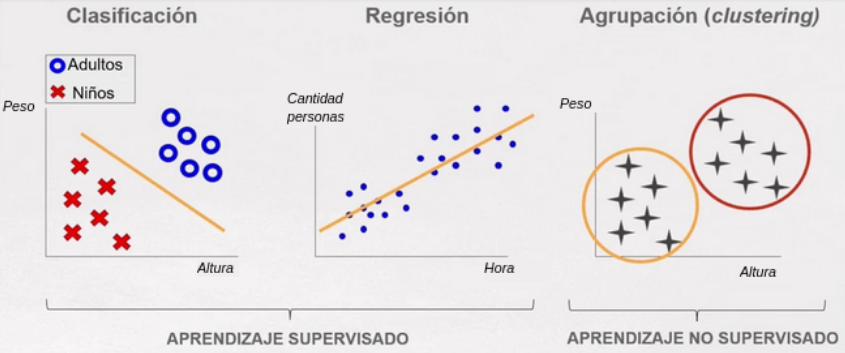
\includegraphics[width=1\textwidth]{images/Clasificacion_algoritmos.png}
  \caption[Tipos de aprendizaje en ML]{Tipos de aprendizaje en ML\protect\footnotemark}  
  \label{fig:Clasif_algoritmos}
\end{figure}

\footnotetext{Sitio Web. \textit{Modelos de Machine Learning}. \url{https://openwebinars.net/blog/modelos-de-machine-learning/}. (Consultado el 30 marzo de 2022).}

\paragraph{Regresión.}

En un problema de regresión se intenta predecir el valor de una variable numérica y continua a partir de un cierto conjunto de datos. 

En general contamos con un set de entrenamiento en el cual conocemos el valor de la variable que queremos predecir. El objetivo es entonces construir un modelo que nos permita predecir el valor de nuestra variable de salida a partir de datos nuevos. Dicho de otra forma, lo que se hace es buscar una función que represente los datos de entrenamiento y que permita generalizar correctamente\footnote{Generalizar es la capacidad de nuestro modelo de ML de obtener buenos resultados con datos nuevos reconociendo patrones generales de los datos de entrenamiento en lugar de reconocer particularidades específicas.}.

El caso más simple es la regresión lineal (observado previamente en la Figura \ref{fig:Clasif_algoritmos}), en el cual nuestro modelo es una recta, la recta que mejor se ajusta a los puntos de nuestro set de entrenamiento. En este ejemplo se intenta predecir la cantidad de personas en un lugar a una hora determinada. 

Los problemas de regresión pueden usarse para realizar distintas predicciones, ya sea el valor de las acciones en el mercado de valores, predecir el costo de una propiedad, estimar las ganancias de un negocio, etc. 

Las claves para identificar un problema de regresión\cite{apunte_uba} son las siguientes:
\begin{itemize}
\item Queremos predecir una variable que es numérica y continua.
\item Contamos con un set de entrenamiento para el cual conocemos el valor de dicha variable.
\end{itemize}

\cleardoublepage
\paragraph{Clasificación.}\label{clasificacion}

En los problemas de clasificación la variable que se intenta predecir no es continua sino discreta, frecuentemente tiene pocos valores posibles y en muchos casos los valores posibles son solo dos: clasificación binaria\footnote{Un caso típico de la clasificación binaria es un problema de análisis de sentimiento, donde queremos saber si un cierto texto es positivo o negativo, es decir si habla bien o mal de un cierto tema. Como set de entrenamiento entonces deberíamos contar con textos para los cuales ya conocemos su sentimiento.}. La idea general es la misma que antes, para este caso contamos con un set de entrenamiento en el cual para cada dato conocemos la clase a la cual pertenece el mismo, y queremos construir un modelo que nos permita clasificar automáticamente datos nuevos cuya clase desconocemos.

Por ejemplo, en la Figura \ref{fig:Clasif_algoritmos}, observamos que tenemos una serie de personas, de las cuales contamos con su peso y altura, y queremos clasificarlas en adultos o niños. Lo que va a hacer un modelo de clasificación es aprender dónde están estos puntos y crear un clasificador que, para nuevos datos de entrada, consiga segmentarlos correctamente en adultos o niños.

Otras aplicaciones, por ejemplo, podrían ser analizar si las reviews de un producto son buenas o malas, medir la actitud del público en general ante determinadas noticias por los comentarios que existen en redes sociales, clasificar si un email es spam o no lo es, etc. 

Las claves para reconocer un problema de clasificación\cite{apunte_uba} son:
\begin{itemize}
\item Queremos determinar la clase / grupo  a la que pertenece cada dato.
\item La clase es una variable discreta con un set de valores posibles limitado y definido.
\item Contamos con un set de entrenamiento para el cual conocemos los datos y a qué clase pertenecen.
\end{itemize}

\cleardoublepage
\paragraph{Agrupación (clustering).}\label{agrupacion}

En un problema de clustering contamos con datos que queremos dividir en grupos de forma automática. Estos datos no tienen etiquetas, no sabemos a qué grupo pertenecen. Lo que hace un algoritmo de clustering es intentar buscar agrupaciones en los datos, creando de esta forma clusters\footnote{Cluster, o grupo, es un conjunto de objetos que son ”similares” entre ellos y ”diferentes” de los objetos que pertenecen a los otros grupos. La palabra cluster viene del inglés y significa agrupación. Desde un punto de vista general, el cluster puede considerarse como la búsqueda automática de una estructura o de una clasificación en una colección de datos no etiquetados.} con características similares. En algunos casos la cantidad de clusters la debemos indicar previamente y en otros el algoritmo es capaz de determinarla por sí mismo.

En el ejemplo de la Figura \ref{fig:Clasif_algoritmos}, podemos ver que se agrupan los puntos de la misma forma que en el problema de clasificación. La diferencia es que en este caso no sabemos si se trata de adultos o niños, sino que es el propio algoritmo el que va a identificar que hay dos grupos, y nosotros somos los que tenemos que interpretar los resultados. 

Otros ejemplos de clustering podrían ser agrupar películas automáticamente de forma que queden juntas las que son de un mismo género; o la detección de comunidades en una red social, el cual es un típico problema de clustering en donde los puntos son los usuarios y queremos agruparlos automáticamente en comunidades. De esta forma podemos descubrir grupos de usuarios que tienen un cierto interés en común aun sin saber exactamente cuál es dicho interés.

Las claves para reconocer un problema de clustering\cite{apunte_uba} son:
\begin{itemize}
\item Contamos con un set de datos y queremos agruparlos en clusters/grupos.
\item No son necesarios labels.
\end{itemize}

\cleardoublepage

\paragraph{Algoritmos más conocidos.}

Resumidamente, en la Figura \ref{fig:Diagrama_algoritmos} se detallan los algoritmos más conocidos para las distintas clasificaciones de machine learning previamente explicadas. 

\begin{figure}[H]    %[H] es para que se ubique justo debajo del texto anterior. 
  \centering
  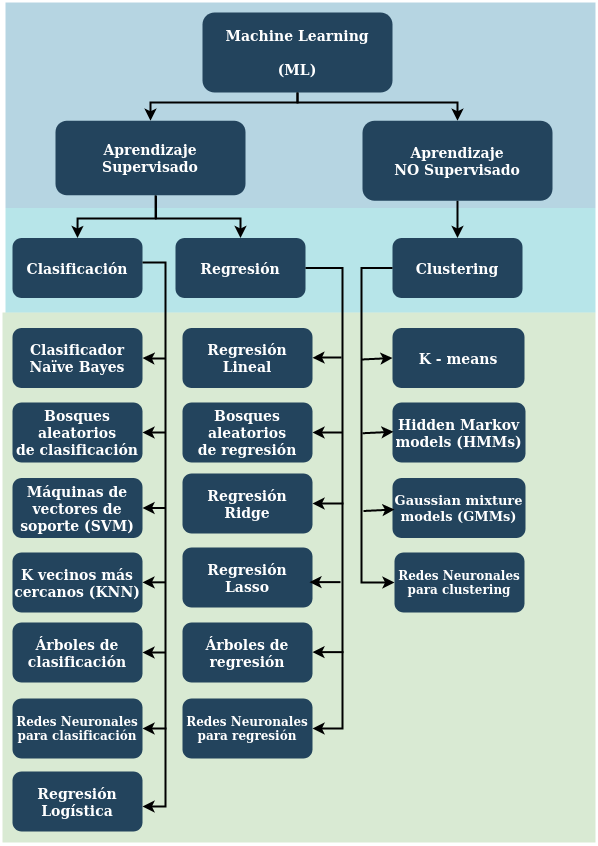
\includegraphics[width=0.8\textwidth]{images/Diagrama_algoritmos.png}
  \caption{Algoritmos de machine learning más conocidos}  
  \label{fig:Diagrama_algoritmos}
\end{figure}

Cabe destacar que algunos algoritmos se pueden adaptar para resolver problemas de otro tipo al cual están inicialmente categorizados. Por ejemplo, KNN que está categorizado como un algoritmo de clasificación, también se puede utilizar para resolver problemas de regresión. Otro caso conocido es Support Vector Regression (SVR), que utiliza las bases de Máquinas de vectores de soporte (SVM) para resolver problemas de regresión.

\cleardoublepage

\subsubsection{Aprendizaje transductivo}

Existe una cierta relación entre los problemas de clustering y de clasificación, por ejemplo dado un problema de clasificación podríamos aplicar clustering primero y luego clasificar a cada punto de acuerdo al cluster al cual pertenece en base a la clase mayoritaria de dicho cluster. Este procedimiento no es muy frecuente pero es conveniente tenerlo en cuenta porque permite entender el funcionamiento de ciertos algoritmos que combinan las propiedades de un problema de clustering y uno de clasificación.

Una aplicación que combina clustering (aprendizaje no supervisado) y clasificación (aprendizaje supervisado) es la que denominamos \textbf{Aprendizaje transductivo}\cite{aprendiz_transd}\cite{apunte_uba} . De esta manera, para predecir nuevos datos no etiquetados se utilizan los datos previamente etiquetados, así como los datos sin etiquetar, como forma de ayuda a un clasificador tradicional.

Consideremos el ejemplo de la Figura \ref{fig:Transductivo_1}. Aquí tenemos solo dos puntos clasificados, uno clasificado como ``blanco'' y el otro como ``negro''. Sin mayor información el punto marcado con el signo de pregunta, cuya clase desconocemos, quedaría clasificado como ``blanco'' ya que está mucho mas cerca del punto blanco que del punto negro.

\begin{figure}[H]    %[H] es para que se ubique justo debajo del texto anterior. 
  \centering
  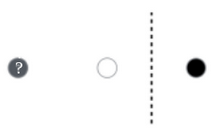
\includegraphics[width=0.5\textwidth]{images/Transductivo_1.png}
  \caption{Aprendizaje transductivo}  
  \label{fig:Transductivo_1}
\end{figure}

En la Figura \ref{fig:Transductivo_2} al agregar puntos cuya clase desconocemos, vemos que en nuestros datos existen dos clusters. De esta manera, si tenemos que asociar cada cluster con un color entonces el de arriba es ``negro'' y el de abajo es ``blanco'', ya que el punto negro pertenece al cluster de arriba y el blanco al de abajo. De este modo, el punto que inicialmente consideramos blanco, con esta nueva información de clusters, sería considerado negro.

\begin{figure}[H]    %[H] es para que se ubique justo debajo del texto anterior. 
  \centering
  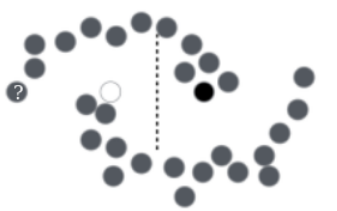
\includegraphics[width=0.5\textwidth]{images/Transductivo_2.png}
  \caption{Aprendizaje transductivo}  
  \label{fig:Transductivo_2}
\end{figure}

El aprendizaje transductivo es un área muy nueva dentro de Data Science y que sin dudas merece ser explorada.

En este Proyecto de Tesis se utilizará el aprendizaje transductivo para lograr inicialmente una clusterización de nuestros candidatos en 5 grupos mediante un algoritmo de clustering (K-means), y luego se realizará una clasificación mediante un algoritmo de clasificación (KNN). 

\subsubsection{Separación de los datos.}\label{Separacion datos}

Dos conceptos importantes que mencionaremos a lo largo del informe son: los “datos de entrenamiento” y los “datos de prueba”.

Como mencionamos anteriormente, los algoritmos de machine learning aprenden de los datos con los que los entrenamos. A partir de ellos, intentan encontrar o inferir el patrón que les permita predecir el resultado para un nuevo caso. Pero, para poder calibrar si un modelo funciona, necesitaremos probarlo con un conjunto de datos diferente. Por ello, en todo proceso de aprendizaje automático, los datos de trabajo se deben dividir mínimamente en dos partes:

\begin{itemize}
\item Los \textbf{datos de entrenamiento} son los datos que usamos para entrenar un modelo. La calidad de nuestro modelo de aprendizaje automático va a ser directamente proporcional a la calidad de estos datos. Por ello son muy importantes las tareas de limpieza y preprocesamiento de los mismos.
\item Los \textbf{datos de prueba o evaluación} son los datos que nos “reservamos” para comprobar si el modelo que hemos generado a partir de los datos de entrenamiento “funciona”.  Es decir, si las respuestas predichas por el modelo para un caso totalmente nuevo son acertadas o no.
\end{itemize}


Es importante que el conjunto de datos de prueba tenga un volumen suficiente como para generar resultados estadísticamente significativos, y a la vez, que sea representativo del conjunto de datos global. Normalmente el conjunto de datos se suele dividir en un \textbf{70\%/80\% de datos de entrenamiento} y un \textbf{30\%/20\% de datos de prueba}, pero se puede variar la proporción según el caso\cite{apunte_uba}. 


\cleardoublepage
\subsubsection{¿Cómo implementar un modelo de ML?}\label{implementar_mod_ML}

Resumidamente, los pasos a seguir para implementar un modelo de ML y utilizarlo para realizar predicciones sobre los datos son los siguientes:
\begin{itemize}
\item Paso 1: Recolección de Datos.
\item Paso 2: Preparación y preprocesamiento de los datos.
\item Paso 3: Elección del modelo de ML.
\item Paso 4: Entrenamiento del algoritmo.
\item Paso 5: Evaluación del modelo.
\item Paso 6: Parameter Tuning o configuración de parámetros.
\item Paso 7: Utilizando nuestro modelo.\\
\end{itemize}

A continuación detallaremos en mayor detalle los mencionados pasos.

\begin{itemize}
\item Paso 1: Recolección de Datos.

Dada la problemática que deseemos resolver mediante algoritmos de ML, nuestro primer paso será recolectar los datos que utilizaremos posteriormente para “alimentar” a dicho algoritmo. 

En este paso hay que tener muy en cuenta la calidad y cantidad de información que consigamos ya que impactará directamente en lo bien o mal que luego funcione nuestro modelo. Estos datos los podemos sacar de bases de datos, planillas de cálculo, utilizando técnicas de web scraping\footnote{Proceso dentro de Data Science que se utiliza para la extracción de datos de sitios web simulando cómo navegaría un ser humano por los mismos.} o mediante APIs\footnote{API o interfaz de programación de aplicaciones, es un conjunto de métodos o funciones que ofrece cierta biblioteca para ser utilizada por otro software como una capa de abstracción.} para recopilar información de manera automática de diversas fuentes de Internet, etc.\\

\item Paso 2: Preparación y preprocesamiento de los datos.

En este paso generalmente se realizan visualizaciones de los datos y se revisa si existen correlaciones entre las distintas “features”\footnote{Features generalmente son las columnas de nuestro dataframe, archivo o base de datos -dependiendo cómo almacenamos nuestros datos-.} de nuestros datos. Al pre-procesar nuestros datos nos referimos a normalizar los mismos: eliminando duplicados y realizando distintas correcciones de errores. El preprocesamiento de datos usualmente tiene un impacto significativo en la performance de generalización de nuestro algoritmo de machine learning\cite{preprocessing}. 

\cleardoublepage
En esta etapa, además, es importante \textbf{separar} nuestros datos en dos grupos:
\begin{itemize}
\item un set de entrenamiento.
\item un set de prueba. 
\end{itemize}

Como mencionamos previamente, el set de test en general es un 20\% o 30\% del set de entrenamiento. Esta partición de los datos en estos dos conjuntos diferenciados permite generar el modelo a partir de los datos de entrenamiento para después comprobar su eficiencia con los datos reservados para test.\\

\item Paso 3: Elección del modelo de ML.

Una vez obtenidos y preprocesados estos datos, lo que se hace es \textbf{elegir el modelo de ML}\footnote{Un modelo de machine learning es la salida de información que se genera cuando se entrena un algoritmo de ML con datos. Después del entrenamiento, al proporcionar un modelo con una entrada, se le dará una salida. Por ejemplo, un algoritmo predictivo creará un modelo predictivo.} de acuerdo al objetivo que tengamos o problema que deseemos resolver. 

De esta manera, utilizaremos algoritmos de clasificación, regresión o clustering para construir nuestro modelo de ML a partir de los datos, de forma tal de luego poder usar dicho modelo para predecir nuevos datos.\\

\item Paso 4: Entrenamiento del algoritmo.

El siguiente paso es \textbf{entrenar} a nuestro algoritmo de ML. En este proceso mediante una serie de iteraciones nuestro algoritmo detecta patrones en nuestros datos que luego nos servirán para poder realizar predicciones con los nuevos datos que se incorporen al sistema.

La idea es entrenar a nuestro algoritmo con el set de entrenamiento (mediante una función \textit{fit()}) para luego, en las etapas posteriores, aplicarlo al set de prueba (mediante una función \textit{predict()}). De esta forma, los datos para los cuales queremos probar el algoritmo (set de test) nunca fueron vistos por el mismo en la etapa de entrenamiento, lo cual permite saber si el modelo fue capaz de generalizar correctamente.\\

\item Paso 5: Evaluación del modelo\cite{apunte_uba}.

Hacer predicciones correctas sobre datos futuros suele ser el principal problema que queremos resolver al utilizar algoritmos de ML. Luego de entrenar el modelo se tiene que \textbf{evaluar} el mismo. Evaluar un modelo, resumidamente, es estimar su rendimiento para saber qué tan bien se desempeñará / predecirá para datos nuevos no vistos por el mismo.

Para poder evaluar un modelo correctamente, tenemos que contar con la separación de nuestros datos en set de entrenamiento y set de prueba que realizamos en los pasos previos. Esto lo hacemos, ya que evaluar la precisión predictiva de un modelo de ML con los mismos datos que se han utilizado para el entrenamiento no es útil, ya que compensa a los modelos que pueden ``recordar'' los datos de entrenamiento en lugar de generalizar.

De esta manera, luego de haber entrenado nuestro modelo de ML, resumidamente lo que hacemos en esta etapa es comparar las predicciones realizadas sobre set de pruebas devueltas por el modelo de ML contra el valor de destino conocido para el mismo set de pruebas; y por último generar alguna \textbf{métrica de evaluación} que nos permite verificar la performance de nuestro modelo indicando la efectividad de las predicciones.

Dependiendo del tipo de modelo que tengamos, podemos utilizar distintas métricas de evaluación para verificar su performance. Como observación, se detallan algunas de las métricas más conocidas en la Tabla \ref{table:1}. \\

\begin{table}[h!]
\centering
\begin{tabular}{|p{6cm}||p{5cm}||p{5cm}|}
\hline
\textbf{Modelos de regresión} & \textbf{Modelos de clasificación} & \textbf{Modelos de clustering} \\ [1ex] 
\hline
Mean square error (MSE)  & Matriz de confusión o error & Inertia \\
\hline
Root MSE (RMSE)  & Accuracy (Exactitud) & Homogeneity \\
\hline
Normalized RMSE (NRMSE)  & Precision (Precisión) & Majority-representation \\
\hline
Mean absolute error (MAE)   & Recall (Sensibilidad o TPR) & Adjusted Rand Index \\
\hline
Mean absolute percentage error (MAPE)  & FP Rate (Especificidad o TNR) & Silhouette coefficient \\
\hline
  &  &  Dunn index \\
\hline
\end{tabular}
\caption{Métricas para evaluar distintos tipos de modelos\cite{metrics_clustering_1, metrics_clustering_2,metrics_clasification,metrics_regression}.} 
\label{table:1}
\end{table}

Por ejemplo, si queremos verificar la performance de un modelo de clasificación podemos utilizar el \textbf{accuracy}. Esta métrica mide el \% de aciertos: es el ratio de las predicciones correctas sobre el número total de instancias evaluadas. Por ejemplo, si el Accuracy es menor o igual al 50\% este modelo no será útil ya que sería como lanzar una moneda al aire para tomar decisiones. Si alcanzamos un 90\% o más podremos tener una buena confianza en los resultados que nos otorga el modelo.\\

\item Paso 6: Parameter Tuning o configuración de parámetros\cite{apunte_uba}.

Si durante la evaluación no obtuvimos buenas predicciones y nuestra métrica de evaluación no logró ser la mínima deseada, es posible que tengamos problemas de overfitting (ó underfitting) y deberemos retornar al paso de entrenamiento (Paso 4) haciendo antes una nueva configuración de hiper-parámetros de nuestro modelo. 

Cada modelo tiene un conjunto de parámetros e hiper-parámetros que necesita para funcionar:
\begin{itemize}
\item Los \textbf{parámetros} son los valores obtenidos por el propio algoritmo a partir de los datos, no son indicados manualmente. 
\item Los \textbf{hiper-parámetros}, en cambio, son datos que debemos pasarle al algoritmo para funcionar. 
\end{itemize}

Como ejemplos de parámetros tenemos los coeficientes en una regresión lineal o logística, o los pesos en una red neuronal artificial. Y como ejemplos de hiper-parámetros, tenemos al ‘k’ en KNN, o los ‘EPOCHs’ que nos permiten incrementar la cantidad de veces que iteramos sobre nuestros datos de entrenamiento en una red neuronal artificial. 

Para encontrar los hiper-parámetros óptimos, es decir, aquellos que mejor funcionan para nuestro set de datos, lo que se hace es, nuevamente, realizar un entrenamiento y una evaluación de nuestro modelo de ML seleccionando e iterando sobre los distintos hiper-parámetros que tengamos: a esto se le conoce como \textit{“Parameter Tuning”}. Esta iteración puede ser de manera aleatoria (método conocido como \textit{random search}) o completa (\textit{grid search}). Luego de realizar esta iteración se obtiene la configuración de hiper-parámetros más óptima.

Algo a tener en cuenta es que, para realizar la evaluación, no debemos usar los datos del set de prueba, ya que podríamos caer en un caso de overfitting seleccionando los parámetros que funcionan mejor para los datos del set de pruebas, pero tal vez no los parámetros que generalicen mejor. Para evaluar el modelo y realizar dicho \textit{“Parameter Tuning”} lo que necesitamos es dividir el set de entrenamiento original en dos: un set de entrenamiento y un \textbf{set de validación}. 

La idea es entrenar el modelo con el set de entrenamiento y luego probarlo con dicho set de validación (NO con el set de pruebas) a efectos de encontrar los mejores hiper-parámetros. El set de validación en general es un 20-30\% del set de entrenamiento original.

Por último, una vez hallados los hiper-parámetros más óptimos, lo que haremos es realizar una \textbf{evaluación final} sobre el set de pruebas con los hiper-parámetros que encontramos, y de esta manera nos dará el accuracy (o la métrica de evaluación que elegimos) para los datos que el modelo no vió.

No obstante, existen 2 problemas con el esquema anterior:
\begin{itemize}
\item Siendo el set de validación siempre el mismo podemos caer en el problema de que los hiper-parámetros que encontremos solo sean óptimos para nuestro set de validación (el cual es un pequeño conjunto de nuestros datos).
\item La división del set de entrenamiento en un nuevo set de entrenamiento y un set de validación hace que haya menos datos disponibles para el entrenamiento. Esto resulta un problema, especialmente para conjuntos de datos pequeños, ya que siempre es mejor utilizar el mayor número de datos posible para el entrenamiento.
\end{itemize}

Para evitar estos 2 problemas utilizamos el método de \textbf{Cross Validation} (o validación cruzada), el cual es prácticamente universal para optimizar algoritmos de ML. Este método nos permite evaluar modelos de ML solucionando los 2 problemas mencionados anteriormente previniendo el overfitting. Para mayor detalle de su funcionamiento ver \textit{\nameref{Cross Validation}}.\\

\item Paso 7: Utilizando nuestro modelo. 

Una vez que obtuvimos buenas predicciones en la etapa de evaluación y nuestra métrica de evaluación llegó a ser la mínima deseada, ya podemos afirmar que estamos en condiciones de utilizar nuestro modelo de machine learning entrenado para realizar predicciones con nuevos datos que están fuera del set de entrenamiento y del set de test.

\end{itemize}


\cleardoublepage
\paragraph{Cross Validation.}\label{Cross Validation}

El método de \textbf{Cross Validation}, o validación cruzada\cite{apunte_uba}\cite{cross_validation}, consiste en entrenar modelos de ML en subconjuntos de los datos de entrada disponibles y evaluarlos con un subconjunto complementario de los datos.

En la la Figura \ref{fig:cross_val} podemos observar el funcionamiento del enfoque básico de Cross Validation: \textbf{k-fold Cross Validation}. Este método comienza particionando el set de entrenamiento en k bloques (o ``folds''). Luego, se realizan varias iteraciones en las cuales entrenamos nuestro algoritmo con k - 1 bloques como set de entrenamiento y lo validamos con el bloque restante (el cual sería nuestro set de prueba), para obtener el valor de alguna métrica de evaluación, como por ejemplo el accuracy. Este proceso se repite k veces con el objetivo de que todos los bloques de datos hayan participado alguna vez del set de pruebas. 

El resultado de la métrica de evaluación final devuelta por k-fold Cross Validation es el \textbf{promedio} de los resultados de dicha métrica de evaluación calculada dentro de las k iteraciones del algoritmo. Esto hay que hacerlo además por cada valor posible para nuestros hiper-parámetros, por lo que, dependiendo de los datos, puede resultar un proceso costoso.

\begin{figure}[H]    %[H] es para que se ubique justo debajo del texto anterior.
 \centering
 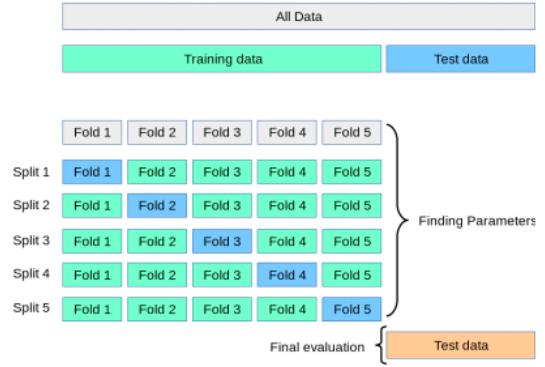
\includegraphics[width=0.8\textwidth]{images/Cross_Validation.png}
 \caption[k-fold Cross Validation.]{k-fold Cross Validation\protect\footnotemark}
 \label{fig:cross_val}
\end{figure}

\footnotetext{Librería Scikit-learn. \textit{Cross-Validation: evaluating estimator performance}. \url{https://scikit-learn.org/stable/modules/cross_validation.html}. (Consultado el 30 marzo de 2022).}

En conclusión, luego de realizar dichas iteraciones mediante k-fold Cross Validation, obtendremos la métrica de evaluación final para cada uno de las combinaciones de nuestros hiper-parámetros, y elegiremos los hiper-parámetros más óptimos (el que mejor métrica de evaluación nos haya dado). 

Una vez hallados los mismos, el último paso, como comentamos con el primer esquema, es realizar una evaluación final sobre el set de pruebas con los hiper-parámetros que encontramos, y de esta manera nos dará el accuracy (o la métrica de evaluación que elegimos) para los datos que el modelo no vió.

Un ejemplo de la utilización de estos esquemas para la evaluación de modelos, lo podemos observar en  \textit{\nameref{IMP_Modelo_clasificacion_KNN}}.\\

\paragraph{Los Problemas de ML: Overfitting y Underfitting.}\label{Over_y_under}

En esta sección vamos a nombrar y explicar algunos de los problemas clave en tareas de ML: overfitting y underfitting. Podemos observar un ejemplo de estos conceptos en la Figura \ref{fig:fitting}.

\begin{figure}[H]    %[H] es para que se ubique justo debajo del texto anterior.
 \centering
 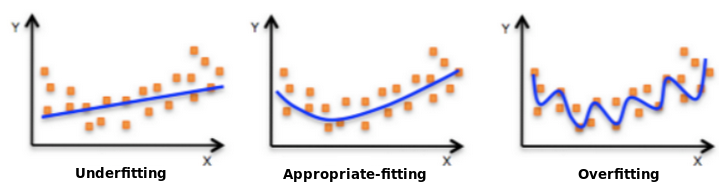
\includegraphics[width=0.9\textwidth]{images/Fitting.png}
 \caption{Overfitting y Underfitting\cite{apunte_uba}}
 \label{fig:fitting}
\end{figure}

\textbf{Overfitting}, o sobre-ajuste, es un problema clave en las tareas de aprendizaje automático supervisado.
Es el fenómeno que se detecta cuando un algoritmo de aprendizaje se ajusta/entrena tan bien al set de datos de entrenamiento que se memorizan el ruido y peculiaridades específicas de los datos de entrenamiento. Entonces, se vuelve difícil para el modelo generalizar a nuevos ejemplos que no estaban en el conjunto de entrenamiento. Es por esto que la precisión del modelo cae cuando se prueba en un conjunto de datos desconocido. De esta manera, termina siendo mayor la precisión en el entrenamiento que la precisión sobre los set de pruebas.

La cantidad de datos utilizados para el proceso de aprendizaje es fundamental en este contexto. Los conjuntos de datos pequeños son más propensos al overfitting que los conjuntos de datos grandes. El ajuste excesivo de los datos de entrenamiento conduce al deterioro de las propiedades de generalización del modelo y da como resultado un rendimiento o precisión del mismo poco fiable\cite{over_and_under}.

El concepto de overfitting está asociado a la complejidad del modelo. Un modelo excesivamente complejo puede ajustar tan bien como queramos al set de entrenamiento pero funcionar muy mal para el set de test\cite{apunte_uba}.

En cambio \textbf{Underfitting}, o sub-ajuste, es el opuesto de Overfitting. Esto ocurre cuando el modelo es incapaz de capturar la variabilidad de los datos. Se produce cuando el modelo es demasiado simple. Si nuestros puntos están distribuidos en forma curva, un modelo lineal es demasiado simple, no tiene el poder expresivo necesario para representar correctamente el set de entrenamiento\cite{apunte_uba}.

Por lo tanto, podemos decir que el modelo óptimo es aquel que tiene la complejidad necesaria para capturar lo que los datos expresan pero no más.

\cleardoublepage

\subsection{K-Nearest Neighbor (KNN).}\label{knn_teoria}

K-Nearest Neighbor o K Vecinos más cercanos (KNN), es un algoritmo ML que se puede usar tanto en tareas de regresión como de clasificación. En nuestra implementación, lo usaremos para resolver un problema de clasificación (ver \textit{\nameref{clasificacion}}). Como mencionamos anteriormente, en los problemas de clasificación la variable que se intenta predecir es discreta. En este tipo de problemas contamos con un set de entrenamiento en el cual para cada dato conocemos la clase a la cual pertenece el mismo, y queremos construir un modelo que nos permita clasificar automáticamente datos nuevos cuya clase desconocemos.

Como lo dice su nombre, el algoritmo KNN se basa en encontrar para un determinado punto m, sus K-vecinos más cercanos. Esto es asumiendo que nuestro set de datos está formado por un conjunto de m puntos en n dimensiones siendo todos los valores numéricos.\\

Para poder utilizar KNN hay que definir previamente dos hiper-parámetros:
\begin{itemize}
\item La métrica a usar para calcular las distancias.
\item El valor de k, es decir cuantos vecinos vamos a considerar.
\end{itemize}

Algo a destacar, es que KNN es un tipo de aprendizaje basado en la memoria, también llamado aprendizaje basado en instancias, que pertenece al aprendizaje perezoso (“lazy learning”). Esto quiere decir que KNN \textbf{no tiene una fase de entrenamiento}. ¿Qué quiere decir que KNN no tenga un proceso de entrenamiento?, y entonces en \textit{\nameref{IMP_Modelo_clasificacion_KNN}} ¿qué se hace realmente al utilizar la función \textit{.fit()} provista por sklearn?. A continuación se contestarán estas preguntas:

\begin{itemize}
\item \textbf{A nivel conceptual}, entrenar un clasificador significa tomar un conjunto de datos como entrada, y obtener a la salida un modelo clasificador identificado con distintos parámetros, los cuales son obtenidos en esta etapa de entrenamiento mediante iteraciones realizando cálculos numéricos o resolviendo problemas de optimización (como por ejemplo la obtención del mejor hiperplano en SVM o el ajuste de los pesos en redes neuronales artificiales). En el caso de KNN, el clasificador no se obtiene luego de iterar y obtener dichos parámetros, sino que se identifica por los propios datos de entrenamiento. Entonces, conceptualmente, entrenar un clasificador KNN simplemente requiere almacenar el conjunto de entrenamiento.

\item \textbf{A nivel de implementación}, evaluar un clasificador KNN en un nuevo punto de datos requiere buscar sus vecinos más cercanos en el conjunto de entrenamiento, lo que puede ser una operación costosa cuando nuestro conjunto de entrenamiento es grande. Existen varios métodos para acelerar esta búsqueda, que generalmente funcionan creando estructuras de datos basadas en el conjunto de entrenamiento. La idea general, es que parte del trabajo computacional necesario para clasificar nuevos puntos es común en todos los puntos. Por lo tanto, este trabajo se puede hacer con anticipación y luego reutilizarse, en lugar de repetirse para cada nueva instancia. De esta manera, en la fase de entrenamiento, al llamar a la función \textit{.fit()} de sklearn, lo que se hace internamente es guardar todo el set de entrenamiento completo mediante estructuras de datos que nos permitan minimizar los futuros cálculos de medición de distancias. Estas estructuras de datos suelen ser árboles kd (\textit{KD tree}) o árboles de bolas (\textit{Ball tree}). De esta manera, posteriormente a utilizar \textit{.fit()} utilizaremos \textit{.predict()}, y en este paso el cálculo de medición de distancias para el nuevo punto a clasificar será mucho más rápido.\\
\end{itemize} 

\subsubsection{Principal limitación KNN.}

Una de las principales limitaciones de KNN\cite{KNN_limitacion} es la \textbf{complejidad computacional requerida al trabajar con datasets de gran tamaño}. 

Esto ocurre debido a que, como mencionamos previamente, cada vez que se va a realizar una predicción para un nuevo punto del set de test, es necesario calcular las distancias entre este punto y todos los demás puntos del set de entrenamiento completo. Dichos cálculos llevan un gran costo computacional si se trata de un dataset de grandes dimensiones. 

Además, KNN requiere almacenar todos los datos de entrenamiento para funcionar, por lo que también existe un gran costo computacional en términos de almacenamiento. Es por esto que se recomienda utilizar datasets de pocas dimensiones para que el clasificador KNN complete su ejecución rápidamente. \\

\subsubsection{Funcionamiento y ejemplo de KNN.}

Luego de haber entrenado / construido nuestro modelo KNN habiendo previamente determinado el valor de k y la métrica de distancia a utilizar, el funcionamiento del algoritmo KNN para la predicción o clasificación de nuevas muestras es el siguiente: 

\begin{itemize}
\item Paso 1: Dado un nuevo punto de entrada del set de pruebas, se calculan las distancias entre este nuevo punto y todos los puntos del set de entrenamiento.
\item Paso 2: Se ordenan las distancias y se determinan los K vecinos más cercanos basándose en los valores mínimos de dichas distancias.
\item Paso 3: Se analiza la clase de esos vecinos y se asigna una clase para ese punto de entrada basado en el voto de la mayoría.
\item Paso 4: Se retorna la clase predicha.
\end{itemize}

En la sección del Anexo \textit{\nameref{anexo_knn}} detallamos un breve ejemplo gráfico en el cual usamos KNN para clasificación utilizando la distancia euclidiana como métrica para calcular las distancias. Viendo este ejemplo podemos observar que KNN se basa esencialmente en un método estadístico. Cuando queremos simplemente clasificar un punto cuya clase no conocemos no hacen falta las probabilidades; podemos simplemente asignarlo a la clase con mayoría entre los k-vecinos del punto.

\cleardoublepage

\subsubsection{Métrica de distancia a emplear.}\label{metrica_dist_emp}

La función de distancia entre dos vectores $x$ e $y$ es una función $d(x,y)$ que define la distancia entre ambos vectores como un número real no negativo. Esta función es considerada como una métrica si satisface las siguientes 4 propiedades\cite{KNN_Ejemplo}: 

\begin{enumerate}
\item Valor no-negativo: La distancia entre $x$ e $y$ siempre es un valor mayor o igual a cero. 
$$d(x,y) \geq 0$$

\item Identidad de los indiscernibles: La distancia entre $x$ e $y$ es igual a cero si y sólo si $x$ es igual a $y$.
\[d(x,y) = 0, \text{   si  } x=y\]

\item Simetría:  La distancia entre $x$ e $y$ es igual a la distancia entre $y$ y $x$.
$$d(x,y) = d(y,x)$$

\item Desigualdad triangular: Considerando la presencia de un tercer punto $z$, la distancia entre $x$ e $y$ es siempre menor o igual que la suma de la distancia entre $x$ y $z$ y la distancia entre $y$ y $z$. 
$$d(x,y) \leq d(x,z) + d(y,z)$$
\end{enumerate}

De esta manera, puede usarse cualquier métrica para medir las distancias en KNN, siempre y cuando cumpla con las propiedades descritas anteriormente.

Dos de las distancias más utilizadas en la implementación de KNN son la distancia euclidiana y la distancia Manhattan. En  Figura \ref{fig:Man_euc} podemos observar gráficamente las diferencias entre las mismas.

\begin{figure}[H]    %[H] es para que se ubique justo debajo del texto anterior.
 \centering
 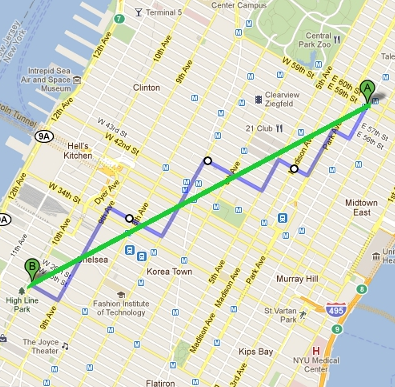
\includegraphics[width=0.6\textwidth]{images/Manhattan_Euclidiana.png}
 \captionsetup{justification=centering,margin=2cm}
 \caption{Distancia Manhattan vs Distancia Euclidiana\cite{apunte_uba}.} 
 \label{fig:Man_euc}
\end{figure}

La \textbf{distancia euclidiana}, o también conocida como Norma L2 o distancia de regla, es una extensión del Teorema de Pitágoras. Esta distancia representa la raíz de la suma al cuadrado de las diferencias absolutas entre los valores opuestos de los vectores. Considerando $x$ e $y$ como vectores a los cuales queremos calcular su distancia euclidiana, su cálculo se obtiene mediante la Fórmula \ref{eq:ecuacion_1}.

\begin{equation}\label{eq:ecuacion_1}
d(x,y)=\sqrt{\sum_{i=1}^{n}|x_{i}-y_{i}|^2}   \qquad  \text{(Ver \cite{KNN_Ejemplo})}
\end{equation}

Donde $x=(x_{1},x_{2},..., x_{n})$, $y = (y_{1},y_{2},...,y_{n})$, y $n = \text{dimensiones de los puntos}$.

En la Fórmula \ref{eq:ecuacion_2} y Figura \ref{fig:KNN_2_Dim} podemos observar el cálculo de la distancia euclidiana entre x e y  considerando un espacio bidimensional. Este es el cálculo que se realiza en la implementación de nuestro KNN, ya que utilizamos la distancia euclidiana como métrica, y únicamente contaremos con 2 ejes.

\begin{equation}\label{eq:ecuacion_2}
d(x,y)=\sqrt{(x_{1}-x_{2})^2 + (y_{1}-y_{2})^2}
\end{equation}

\begin{figure}[H]    %[H] es para que se ubique justo debajo del texto anterior.
 \centering
 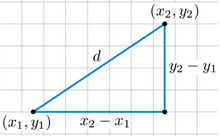
\includegraphics[width=0.4\textwidth]{images/KNN_2_Dim.png}
 \captionsetup{justification=centering,margin=2cm}
 \caption{Distancia Euclidiana en 2 dimensiones.} 
 \label{fig:KNN_2_Dim}
\end{figure}

En cambio, la \textbf{distancia Manhattan}\footnote{Su nombre es debido a que es la forma de calcular distancias en una ciudad con forma de grilla en la cual solo nos podemos mover por las calles en forma horizontal y vertical}, o también conocida como Norma L1 o distancia rectilínea, se calcula como la sumatoria de la diferencia absoluta entre los valores opuestos de los vectores.  Considerando $x$ e $y$ como vectores a los cuales queremos calcular su distancia Manhattan, su cálculo se obtiene mediante la Fórmula \ref{eq:ecuacion_3}.

\begin{equation}\label{eq:ecuacion_3}
d(x,y)=\sum_{i=1}^{n}|x_{i}-y_{i}|  \qquad  \text{(Ver \cite{KNN_Ejemplo})}
\end{equation}

Donde $x=(x_{1},x_{2},..., x_{n})$, $y = (y_{1},y_{2},...,y_{n})$, y $n = \text{dimensiones de los puntos}$.

\cleardoublepage
\subsubsection{Eligiendo el valor de k: overfitting y underfitting.}

En el caso de KNN el único hiper-parámetro que manejamos -además de la métrica usada para la distancia-, es $k$. La elección del valor $k$ tendrá un impacto significativo en los resultados del algoritmo. 

Para determinar el valor óptimo para $k$ lo que se hace es probar diferentes valores de $k$ y ver cual es el que nos da mejores resultados. Aquí hay que tener un cierto cuidado ya que hay que entender qué implica aumentar o disminuir la cantidad de vecinos más cercanos.
Veamos en la Figura \ref{fig:KNN_k_1} qué pasa cuando usamos $k = 1$, es decir cuando a cada punto lo clasificamos únicamente en base al punto más cercano.

\begin{figure}[H]    %[H] es para que se ubique justo debajo del texto anterior.
 \centering
 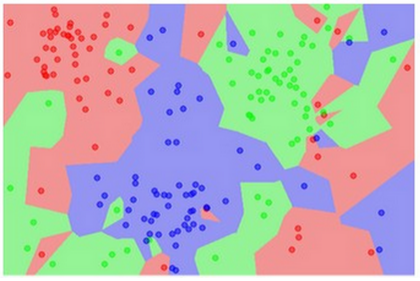
\includegraphics[width=0.7\textwidth]{images/KNN_k_1.png}
 \captionsetup{justification=centering,margin=2cm}
 \caption{KNN con k = 1. \cite{apunte_uba}} 
 \label{fig:KNN_k_1}
\end{figure}

En este caso nuestro el set de entrenamiento en KNN es simplemente perfecto porque dado un registro cualquiera, el más parecido es el registro mismo y, por lo tanto, vamos a tener 100\% de precisión para el set de entrenamiento. Sin embargo, esto no quiere decir que el algoritmo generalice bien y para el set de pruebas los resultados pueden ser catastróficos.

Lo que podemos ver es que la distribución que aprende nuestro clasificador no es homogénea, es decir que hay puntos de distintas clases mezclados en zonas en las cuales predomina otra clase, esto implica que nuestro clasificador va a funcionar muy bien para el set de entrenamiento pero no aprendió a generalizar y esto quiere decir que no va a ser muy bueno para predecir la clase de puntos nuevos que no hayamos observado en el set de entrenamiento. Esta es la definición de overfitting que discutimos en la sección previa (Ver \textit{\nameref{Over_y_under}}): cuando un algoritmo funciona bien para el set de entrenamiento y mal para datos nuevos. El concepto es que aprender a predecir el set de entrenamiento no es lo mismo que aprender a generalizar.

\cleardoublepage
Ahora veamos en la Figura \ref{fig:KNN_k_5} qué sucede con $k = 5$.

\begin{figure}[H]    %[H] es para que se ubique justo debajo del texto anterior.
 \centering
 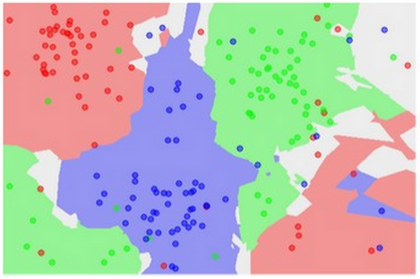
\includegraphics[width=0.7\textwidth]{images/KNN_k_5.png}
 \captionsetup{justification=centering,margin=2cm}
 \caption{KNN con k = 5. \cite{apunte_uba}} 
 \label{fig:KNN_k_5}
\end{figure}

Como podemos ver en la Figura \ref{fig:KNN_k_5} el clasificador aprendió a generar áreas más suaves y por consiguiente es un clasificador que generalizará mejor para predecir puntos que no estaban en el set de entrenamiento. Podriamos pensar entonces que es conveniente usar valores de k grandes como $k = 1000$ o incluso $k = n$ (donde $n$ es la cantidad de puntos de datos del set de entrenamiento). Sin embargo, al aumentar el valor de $k$ estamos dando cada vez mayor peso a las clases que tienen mayor cantidad de puntos en el set de entrenamiento, en el extremo si $k = n$ vamos a predecir para todos los puntos la clase que mayor cantidad de puntos tiene en el set de entrenamiento lo cual no es bueno. 

En resumen:
\begin{itemize}
\item Cuando $k$ es muy bajo, el algoritmo toma muy pocos puntos para clasificar un punto nuevo. Es un caso de overfitting. El modelo clasifica los puntos nuevos en base a muy poca evidencia. Nuestro algoritmo alucina, las fronteras se vuelven muy complejas, demasiado complejas para el set de datos que tenemos. 
\item Cuando $k$ es un número muy grande, KNN considera demasiados puntos para clasificar un punto nuevo. Este es un caso de underfitting, donde nuestro algoritmo tiene visión borrosa por estar mirando demasiados puntos, las fronteras entre nuestras clases se vuelven difusas y el poder expresivo del algoritmo es pobre. 
\end{itemize}

En definitiva, el $k$ óptimo en KNN es aquel que nos de un buen desempeño en cuanto a la precisión de clasificación para el mayor k posible. Una de las mejores formas para seleccionar nuestro $k$ óptimo, es utilizando el método de \textbf{Cross Validation} (ó validación cruzada): ver \textit{\nameref{Cross Validation}}.

\cleardoublepage
\subsection{K-means.}\label{k_means_3_4}
K-means o K-medias, o también conocido como algoritmo de Lloyd, es un algoritmo de ML de clustering (ver \textit{\nameref{agrupacion}}). Como mencionamos anteriormente, en problemas de clustering contamos con datos que queremos dividir en grupos de forma automática. Estos datos no tienen etiquetas, no sabemos a qué grupo pertenecen. K-means nos permite encontrar cómo repartir m puntos en n dimensiones dentro de k clusters.

El nombre de K-means viene porque representa cada uno de los clusters por la media de sus puntos, es decir, por su centroide. Cada clúster, por tanto, es caracterizado por su centroide que se encuentra en el centro de los elementos que componen el clúster.

Para este algoritmo, el único hiper-parámetro que se necesita definir previamente es k, el número de clusters. Este k se puede obtener de distintas formas, en nuestra implementación utilizaremos el \textit{método del codo} para calcularlo. 

A continuación explicaremos en qué consiste este método, detallando el funcionamiento de k-means, su objetivo, sus desventajas y las mejoras que se pueden aplicar.

\subsubsection{Funcionamiento y ejemplo de K-means.}\label{K_means_funcionamiento}

Resumidamente, habiendo definido previamente nuestro k, el número de clusters, y teniendo como entrada nuestros puntos de datos $x_{1},...,x_{m}$, el funcionamiento de K-means consta de los siguientes 4 pasos\cite{K_means_review}:

\begin{itemize}
\item Paso 1: Se inicializan aleatoriamente los centroides $C_{1},...,C_{k}$ colocándose en posiciones al azar. Cada centroide $C_{j}$ pertenece a un cluster $j$ específico. 
\item Paso 2: Se asignan los puntos de datos a su cluster más cercano: Para esto, lo que se hace es, para cada punto de datos $x_{i}$, se calculan las distancias euclidianas con cada uno de los centroides $C_{j}$. Luego, se asigna cada punto de datos $x_{i}$ al cluster $j$, cuyo centroide $C_{j}$ es el más cercano al punto $x_{i}$ basándose en la mínima distancia euclidiana. Matemáticamente. se utiliza la Fórmula \ref{eq:ecuacion_1} para calcular la distancia euclidiana entre cada uno de nuestros puntos de datos $x_{i}$, y cada uno de nuestros centroides $C_{j}$, y obtener el mínimo valor. Reformulando dicha ecuación, nos quedaría la Fórmula \ref{eq:ecuacion_4}.   

\begin{equation}\label{eq:ecuacion_4}
d(x,C_{j})=\sqrt{\sum_{i=1}^{d}|x_{i}-C_{ji}|^2}  \qquad  \text{(Ver \cite{K_means_experiment})}
\end{equation}

Donde $d = \text{dimensiones de nuestros puntos de datos}$, $x_{i} = (x_{1},x_{2},...,x_{d})$ la posición de un punto $x$ de nuestro set de datos para la dimensión $i$, y $C_{ji} = (C_{11},C_{12},...,C_{kd})$ la posición de nuestro centroide $C$ del cluster $j$ para la dimensión $i$.
            
En la Fórmula \ref{eq:ecuacion_4}, podemos visualizar que los centroides tienen igual cantidad de dimensiones que nuestros puntos y, además, pueden o no coincidir con puntos de los datos. Un centroide que es también un punto de los datos se lo llama “clusteroid”. En general, no se pide que los centroides sean también puntos sino que se permite que tomen cualquier posición dentro del espacio de los datos.

\item Paso 3: Se actualizan las posiciones de los $C_{j}$ (centroides $C$ pertenecientes a los clusters $j$). De esta manera, se recalculan los centroides como el promedio de todos sus puntos (los que pertenecen a su cluster) de forma tal de minimizar la distancia desde el centroide a los puntos asignados al mismo. Como resultado, los centroides se mueven al centro promedio de los puntos a los que se les asignaron. Matemáticamente. se utiliza la Fórmula \ref{eq:ecuacion_5} para calcular, para cada cluster $j=(1,...,k)$ la nueva posición del centroide $C_{j}$, el cual se calcula como el promedio de todos los puntos $x_{i}$ asignados al cluster $j$ en el paso anterior.  

\begin{equation}\label{eq:ecuacion_5}
C_{j}(a)=\frac{1}{m_{j}}\sum_{x_{i} \in C_{j}}^{x_{m}}x_{i}(a),     \text{   para  } a = (1,...,d)
\end{equation}

Donde $d = \text{dimensiones de nuestros puntos de datos y centroides}$, $m_{j}$ = cantidad de puntos de nuestro set de datos pertenecientes al cluster $j$, $x_{i}(a)$ = posición de nuestro punto del set de datos $x_{i}$ para la dimensión $a$, y $C_{j}(a)= (C_{1}(1),C_{1}(2),...., C_{K}(D))$ la posición de nuestro centroide $C$ del cluster $j$ para la dimensión $a$.

\item Paso 4: Se repiten los pasos 2 y 3 hasta que los centroides convergen. La convergencia puede verificarse mediante la diferencia entre los centroides entre el paso anterior y el actual. Cuando los centroides prácticamente ya no cambian de posición o cuando los puntos de datos no cambian de cluster se declara la \textbf{convergencia} del algoritmo.\\

\end{itemize}

A modo de ejemplo, en la sección del Anexo \textit{\nameref{anexo_k_means}}, detallamos un ejemplo gráfico en el cual utilizamos K-means para clusterizar nuestros datos hasta llegar a su convergencia. 

\cleardoublepage

\subsubsection{Objetivo de k-means y su función de coste.}

El objetivo de K-means es encontrar cómo repartir m puntos en n dimensiones dentro de k clusters de la “mejor forma posible”. 

¿A qué llamamos “de la mejor forma posible”?: se puede definir a cada cluster a partir de su centro (centroide), en cuyo caso la mejor distribución posible es aquella que minimiza la distancia entre cada punto del cluster y el centroide que se le asignó. Esto es lo que se conoce como \textbf{Inercia} (Inertia) o \textbf{WCSS} (within-cluster sum-of-squares, suma de cuadrados intra cluster), y es lo que busca \textit{minimizar} K-means.

A este criterio de Inercia también se lo considera como la \textbf{función de coste J}\footnote{La función de coste o también llamada función de distorsión u objetivo, es una función que trata de determinar la diferencia o el error entre el valor estimado / predicho por un modelo de machine learning y el valor real, con el fin de optimizar los parámetros en dicha función y obtener un error mínimo. En el caso de k-means, nuestros valores estimados son las posiciones de los centroides -los cuales tenemos que descubrir y encontrar los más óptimos / los que minimicen nuestra J- y nuestros valores reales son nuestros puntos del cluster.} de K-means, la cual se intenta \textit{minimizar}. 

Dicho de otra manera, el objetivo de k-means es encontrar la ubicación de los centroides que minimicen la inercia, esta será la posición óptima de los mismos.

La Inercia\cite{K_means_experiment} se puede reconocer como una medida de la coherencia interna de los clústeres, permitiendo medir qué tan bien K-means realiza la agrupación del conjunto de datos. La misma se calcula como la sumatoria de las diferencias de las distancias (generalmente euclidiana) al cuadrado entre cada uno de los puntos de datos $x_{i}$ pertenecientes a un cluster $j$ y el centroide al que fue asignado dicho punto, $C_{j}$: Fórmula \ref{eq:ecuacion_6}.

\begin{equation}\label{eq:ecuacion_6}
J = Inertia = WCSS = \sum_{C_{j}}^{C_{k}}  ( \sum_{xi \in C_{j}}^{x_{m}}||x_{i}-C_{j}||^2)
\end{equation}

Donde $k$ = número de centroides ó clusters, $m$ = cantidad de puntos de nuestro set de datos, $C_{j}$ = centroide de cluster $j$, y $x_{i}$ = punto $i$ de nuestro set de datos asignado a $C_{j}$. Además, el término $||x_{i}-C_{j}||$ se corresponde a la distancia euclidiana entre cada punto del set de datos, $x_{i}$, y el centroide que tiene asignado, $C_{j}$. Este cálculo se corresponde a la Fórmula \ref{eq:ecuacion_4} que obtuvimos anteriormente.

Considerando una inicialización aleatoria de nuestros centroides, y por ejemplo, definiendo que nuestro número de clusters es 3 ($k$ en kmeans = 3), entonces la Fórmula \ref{eq:ecuacion_6} se podría reescribir como la Fórmula \ref{eq:ecuacion_7}. Podemos observar que al variar la inicialización de nuestros centroides, las posiciones de nuestros $C_{j}$ cambiarían, por lo que nuestra $WCSS$ sería distinta. 

\begin{equation}\label{eq:ecuacion_7}
WCSS =  \sum_{x_{i} \in C_{1}}||x_{i}-C_{1}||^2 + \sum_{x_{i} \in C_{2}}||x_{i}-C_{2}||^2 + \sum_{x_{i} \in C_{3}}||x_{i}-C_{3}||^2     \qquad  \text{(Ver \cite{K_means_elbow})}
\end{equation}

\cleardoublepage
Es importante entender la Fórmula \ref{eq:ecuacion_6} para comprender el problema genérico de clustering. Se sabe que hay k centroides y que cada uno de estos centroides puede estar en cualquier punto del espacio. El objetivo de k-means es \textbf{encontrar la posición óptima para estos centroides de forma tal de minimizar la distancia total entre los puntos y los centroides que se le han asignado}. Es evidente que cada punto debe estar asignado a su centroide más cercano para minimizar la distancia por lo que el problema puede resumirse a \textbf{encontrar la posición óptima para los k centroides}.

Obtener el mínimo valor de nuestro $WCSS$, o que es lo mismo que encontrar el mínimo global, es un proceso muy complejo debido a la inmensa cantidad de formas en las que nuestros m puntos de datos se pueden repartir en k clusters. En lugar de esto, k-means trata de encontrar una solución que, aun no siendo la mejor de entre todas las posibles, sea buena (óptimo local) y garantice un agrupamiento en el que los clusters sean poco dispersos y se encuentren separados entre sí.

Es de destacar que, suponiendo que tenemos $m$ puntos de datos y especificamos que este $m$ sea nuestro número de clusters ($k$ = $m$), entonces $WCSS$ será 0 ya que cada punto de nuestros datos actuará como centroide de sí mismo y la distancia euclidiana entre ellos será nula. De esta forma, cada cluster contendrá solo un punto. Esto idealmente es un cluster perfecto, pero no tiene ningún sentido tener tantos clusters como puntos de datos tengamos. Por lo tanto, existe un valor de umbral para $k$ que podemos encontrar utilizando el \textit{método del codo}, el cual veremos más adelante en \textit{\nameref{Elbow_Met}}).

\cleardoublepage
\subsubsection{Limitaciones K-means.}\label{limit_kmeans}

K-means tiene tres principales limitaciones, las cuales describiremos a continuación.

\begin{enumerate}

\item \textbf{Outliers}: Un outlier es una observación atípica dentro de una muestra de datos que es notablemente diferente del resto. Los outliers representan errores en la medición, mala recolección de datos, o simplemente muestran variables no consideradas al recolectar los datos.
En k-means los outliers pueden incrementar la función de coste o Inercia. Varios investigadores observaron que, cuando los datos contienen outliers, existe una variación en el resultado que significa que no hay un resultado estable al realizar diferentes ejecuciones de k-means con los mismos datos\cite{K_means_review}. Por esta razón, es muy importante eliminar los outliers de nuestro conjunto de datos. Los valores atípicos se pueden eliminar aplicando técnicas de preprocesamiento en el conjunto de datos original.

\item \textbf{Número de los $k$ clusters}: Uno de los principales inconvenientes de K-means es la necesidad de determinar el número óptimo de los $k$ clusters por adelantado. Esto perjudica la eficacia del algoritmo ya que en la práctica, no se conoce a priori el número de clusters final. Este defecto lo perjudica al compararlo con otros algoritmos, ya que en muchos la inicialización del número de clusters no es necesaria. Todavía es un problema saber cuál es el número correcto de $k$ clusters que debemos asignar\cite{K_means_review}.

\item \textbf{Inicialización de los centroides}: La selección inicial de los centroides dirige el proceso de K-means y las particiones resultantes y su efectividad están condicionadas a la elección de estos centroides\cite{K_means_experiment}. Esto lo podemos ver en mayor detalle en la sección del Anexo \textit{\nameref{anexo_pos_inic_centroides}}. Existen numerosos estudios\cite{K_means_initial_centroids} que muestran que la performance de K-means es fuertemente dependiente de la estrategia de inicialización de la ubicación de los centroides a utilizar.

\end{enumerate}

Todas estas limitaciones descritas anteriormente fueron abordadas y resueltas en la implementación de k-means realizada para este Proyecto de la siguiente forma:

\begin{itemize}

\item Para el primer problema, los outliers, se aplicó un pre-procesamiento de nuestros datos que permitió removerlos: ver \textit{\nameref{IMP_Modelo_clasificacion_KNN}}.

\item Para el problema de la determinación óptima y por adelantado del número de los $k$ clusters, se aplicó el \textit{método del codo}: ver \textit{\nameref{Elbow_Met}}.

\item Para el último caso de inicialización de los centroides, como se menciona en \textit{\nameref{anexo_pos_inic_centroides}}, una de las soluciones para no caer en un mínimo local malo es realizar varias ejecuciones de K-means con inicializaciones aleatorias para los centroides, computar la función de distorsión J para cada resultado final y quedarnos con el mínimo. 

En la implementación de esta Tesis, se utilizó una estrategia más novedosa, inicializar nuestros centroides utilizando K-means++: ver \textit{\nameref{k_means_plus_plus}}. La ventaja de utilizar esta estrategia es que generalmente funciona mejor y más rápido que la detallada anteriormente, por lo que actualmente es uno de los métodos estándar para inicializar nuestros centroides en k-means. \cite{K_means_plus_plus}
\end{itemize}

\cleardoublepage
\paragraph{Obtención del k mediante Elbow Method.}\label{Elbow_Met}

Como se mencionó anteriormente, es necesario encontrar el valor óptimo de $k$. Un buen modelo k-means es uno que tenga la menor Inertia y un bajo número de clusters $k$. Sin embargo esto no es posible, ya que si $k$ aumenta, Inertia decrece.

\textit{Elbow method} o \textit{método del codo} nos permite determinar el óptimo valor de $k$, o dicho de otra forma, el óptimo número de clusters en los cuales nuestros puntos de datos serán clusterizados. Mediante este método lo que se hace es graficar cómo varía la función de costo o Inercia en función de $k$: recordemos que la Inercia se calcula mediante la Fórmula \ref{eq:ecuacion_6}. 

Luego de obtener este gráfico, se encuentra el punto ``del codo'', el cual indicará nuestro $k$ óptimo. Este es el punto después del cual la Inercia comienza a disminuir de forma lineal, o dicho de otra forma, el punto ``del codo'' indica que después de este punto, el cambio en la disminución del valor de la Inercia no es significativo. 

Veamos el siguiente ejemplo donde obtendremos nuestro $k$ óptimo en base al \textit{método del codo}: para los puntos de datos observados en la Figura \ref{fig:Elbow_1}, podemos observar visualmente 3 clusters separados, por lo que el número óptimo de clusters debería ser 3. En este caso es bastante sencillo observar esto, pero hay muchos casos donde no es fácil visualizar a simple vista el número de $k$ óptimo, y es por esto que el \textit{método del codo} es de gran utilidad. 

Utilizando esta técnica, graficamos la Inertia en función de $k$: iteramos valores de $k$ desde 1 hasta 9 y calculamos los valores de inercia para cada valor de $k$ dentro de ese rango, obteniendo el gráfico de la Figura \ref{fig:Elbow_2}.

\begin{figure}[H] %[H] es para que se ubique justo debajo del texto anterior.
\begin{minipage}[b]{0.5\linewidth}
\centering
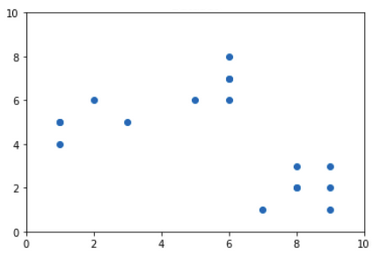
\includegraphics[width=\linewidth]{images/Elbow_1.png}
\caption{Puntos de datos.}
\label{fig:Elbow_1}
\end{minipage}
\hspace{0.5cm}
\begin{minipage}[b]{0.5\linewidth}
\centering
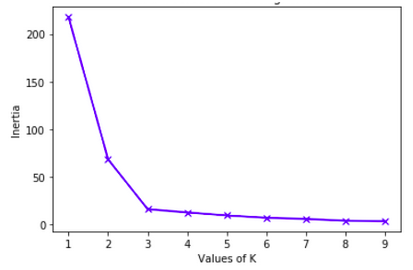
\includegraphics[width=\linewidth]{images/Elbow_2.png}
\caption{Método del codo usando Inercia.}
\label{fig:Elbow_2}
\end{minipage}
\end{figure}
 
De esta manera, concluimos que, para estos datos, viendo el gráfico de la Figura \ref{fig:Elbow_2}, el punto ``del codo'' está en $k=3$, siendo 3 nuestro $k$ óptimo. 

\cleardoublepage
En la Figura \ref{fig:Elbow_3} podemos visualizar los puntos de datos clusterizados para diferentes valores de $k$, observando de esta manera que con $k=3$ obtenemos la clusterización más óptima y lógica.

\begin{figure}[H]    %[H] es para que se ubique justo debajo del texto anterior.
 \centering
 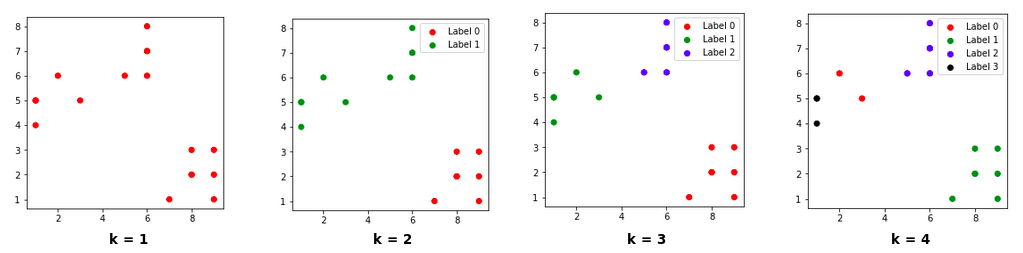
\includegraphics[width=1\textwidth]{images/Elbow_3.png}
 \captionsetup{justification=centering,margin=1cm}
 \caption{Puntos de datos clusterizados para diferentes valores de $k$.}
 \label{fig:Elbow_3}
\end{figure} 

\paragraph{Inicialización de los centroides: k-means++.}\label{k_means_plus_plus}

K-Means++\cite{K_means_plus_plus} es una variante de K-Means en donde lo único que cambia con respecto a este es la forma en que se inicializan los centroides (el paso 1 de k-means descrito en la sección \textit{\nameref{K_means_funcionamiento}}). Actualmente es uno de los métodos estándar para inicializar los centroides en k-means.

De esta manera, habiendo predefinido nuestro $k$, los pasos para inicializar nuestros centroides con k-means++ son:

\begin{enumerate}
\item Se elige un punto al azar perteneciente a nuestros datos como primer centroide. Este paso es el mismo que ocurre en k-means, solo que en este caso únicamente el primer centroide será elegido al azar.
\item Calculamos la distancia $D(x)$ entre cada punto de nuestros datos $x$ y su centroide. 
\item Uno de nuestros puntos de datos $x$ será elegido como el nuevo centroide. Este nuevo centroide será el que tenga la mayor distancia al cuadrado $D(x)^2$ con respecto a su centroide, es decir, el punto $x$ que tenga la distancia más lejana con su centroide. 
\item Repetimos los pasos 2 y 3 hasta que nuestros $k$ centroides sean asignados.
\end{enumerate}

La idea de K-means++ es asignar los centroides de forma espaciada, de esta forma el óptimo local obtenido por K-Means tiene una mayor probabilidad de estar cerca del óptimo global.

\cleardoublepage
En la secuencia de la Figura \ref{fig:K_means_plus_plus} podemos observar un ejemplo de asignación de centroides por medio de k-means ++, habiendo previamente definido $k=3$. Observamos que, a partir de la muestra de datos \textbf{(1)}, obtendremos la inicialización de nuestros centroides \textbf{(6)}.\\

\begin{figure}[H]    %[H] es para que se ubique justo debajo del texto anterior.
 \centering
 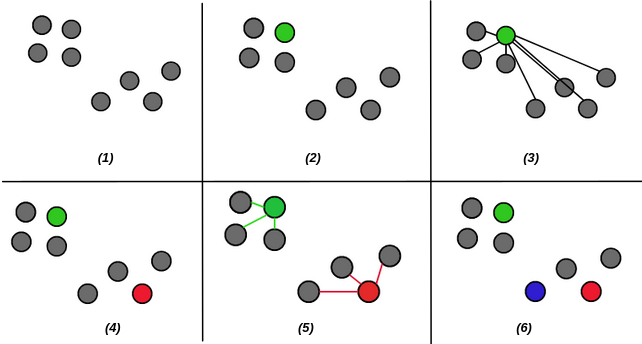
\includegraphics[width=0.8\textwidth]{images/K_means_plus_plus.png}
 \captionsetup{justification=centering,margin=1cm}
 \caption{Inicialización de centroides mediante K-means.}
 \label{fig:K_means_plus_plus}
\end{figure} 

En \textbf{(2)} se elige aleatoriamente un punto al azar como centroide inicial (en este caso el punto verde).
En \textbf{(3)} se calcula la distancia $D(x)$ entre cada uno de los puntos $x$ y su centroide. Para este caso únicamente tenemos el centroide verde. 
En \textbf{(4)} se encuentra al segundo centroide (rojo) de manera que esté alejado del centroide verde. Este segundo centroide es el punto x que tiene la mayor distancia al cuadrado $D(x)^2$ a su centroide.
En \textbf{(5)} se calculan nuevamente las distancias $D(x)$ entre cada uno de los puntos y su centroide más cercano.
Por último, en \textbf{(6)} finalizamos la inicialización de nuestros centroides encontrando al último y tercer centroide (azul). El mismo fue elegido ya que su punto $x$ es el que tiene la mayor distancia al cuadrado $D(x)^2$ a su centroide con respecto a cualquier otro punto y su centroide.

De esta manera, concluimos que K-means++ genera una inicialización más dispersa de los centroides iniciales comparándolo con el método de K-means estándar de inicialización aleatoria. El problema de K-Means++ es que para datos realmente masivos necesita hacer k iteraciones sobre los datos para elegir los centroides, tarea que es todavía más ineficiente cuando k es un número largo. Sin embargo, en general, K-Means++ genera una inicialización mejor para K-Means y esto permite no solo obtener una mejor solución final sino que también acelera la velocidad de convergencia del algoritmo.

\cleardoublepage
\subsection{Redes Neuronales Artificiales (ANN).}\label{ann_teoria}

Las redes neuronales artificiales (o artificial neural network, ANN) son técnicas de Machine Learning que permiten imitar o reproducir la capacidad de aprender propia del comportamiento de un cerebro humano. Las ANN están compuestas por un conjunto de elementos simples (neuronas artificiales) que se interconectan masivamente en paralelo y con organización jerárquica\cite{ANN_21}.

En esta sección detallaremos el funcionamiento básico y los componentes de una red neuronal; la cual será utilizada como base en la implementación del modelo Word2vec para obtener word embedddings: Ver \textit{\nameref{Implementacion_word_emb_y_wmd}}.

Existen muchísimos modelos de redes neuronales, los cuales pueden ser entrenados para resolver distintas tareas, tanto de clasificación o de regresión, como de clustering. En esta sección se explicarán dos de ellos, el modelo más básico y simple de una red neuronal, conocido como \textit{Perceptrón simple}, y su modelo predecesor, \textit{Perceptrón Multicapa} (o también conocido como Multi Layer Perceptron, \textit{MLP}). Ambos modelos son considerados como algoritmos de clasificación, formando parte de la rama de aprendizaje supervisado.

\subsubsection{Perceptrón simple.}

El Perceptrón Simple es un algoritmo de clasificación lineal que surge a fines de la década del 50 y fue desarrollado por Frank Rosenblatt. En aquel tiempo se buscaba crear un algoritmo que imitase el funcionamiento del cerebro humano. El perceptrón puede verse biológicamente como una neurona, siendo la unidad básica de procesamiento que se encuentra en una red neuronal. La teoría era que un perceptrón (o neurona) podía programarse como una salida binaria que dependía del resultado de la combinación lineal entre las entradas y pesos asignados a las mismas. De esta forma, la neurona respondía de manera binaria (0 ó 1) según si el resultado de la combinación lineal fuese mayor o menor a un cierto umbral mediante el uso de una “función de activación”\cite{apunte_uba}, la cual detallaremos más adelante.

En resumen, esta neurona (o perceptrón) tiene conexiones con nodos de entrada, a partir de los cuales recibe estímulos externos (valores de entrada). Con estos valores la neurona realiza un procesamiento interno y genera un valor de salida, decidiendo de esta manera a cuál de las dos clases posibles pertenece la observación\cite{ANN_21}. Este procesamiento depende de las distintas funciones / cálculos matemáticos llevados a cabo mediante la \textit{función de entrada} y la \textit{función de activación} de la neurona (o también llamada \textit{función de transferencia})\cite{ANN_22}. Podemos observar un diagrama de la arquitectura del Perceptrón Simple en la Figura \ref{fig:ann_1}. 

\begin{figure}[H]    %[H] es para que se ubique justo debajo del texto anterior.
 \centering
 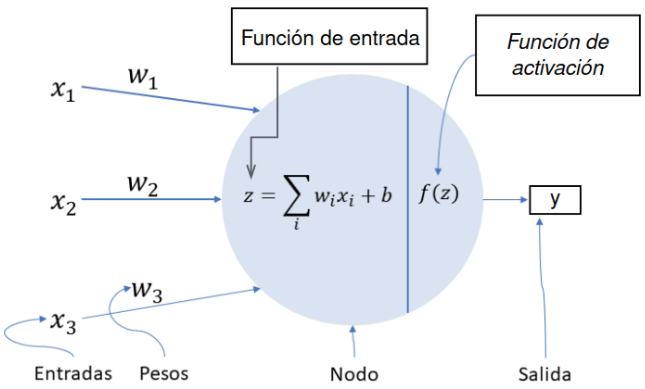
\includegraphics[width=0.8\textwidth]{images/ANN/1-ANN.png}
 \caption{Modelo Perceptrón Simple} 
 \label{fig:ann_1}
\end{figure}

Mencionaremos las partes involucradas en dicho esquema:
\begin{itemize}
\item \textbf{Entradas ($x_1, x_2, x_3, x_n$)}: Las \textit{entradas} son los valores de entrada a la neurona que provienen de estímulos externos. 

\item \textbf{Pesos ($w_1, w_2, w_3, w_n$)}: Los \textit{pesos} son los coeficientes que determinan la intensidad o fuerza de la conexión de las señales de entrada registradas por la neurona. Si el peso de una entrada $x_1$ es mayor al peso de la entrada $x_2$, entonces la entrada $x_1$ tiene mayor influencia en la neurona. Si el peso es positivo se habla de una \textit{excitación} de la entrada, en cambio si el peso es negativo se habla de una \textit{inhibición} de la misma.

\item \textbf{Función de entrada}: En esta parte del esquema se aplica una función de entrada a nuestros valores de entrada, sus pesos y el bías -representado en la Figura como $b$\footnote{El bias o sesgo es el término independiente que permite cambiar o disparar la función de activación para garantizar un aprendizaje exitoso. En otras palabras, permite controlar qué tan predispuesta está la neurona a disparar un 1 o un 0 independientemente de los pesos. Un sesgo alto hace que la neurona requiera una entrada más alta para generar una salida de 1. Un sesgo bajo lo hace más sencillo.}-.

Existen distintas funciones de entrada, tales como la sumatoria de las entradas ponderadas, la productoria de las entradas ponderadas o el máximo de las entradas ponderadas\cite{ANN_23}. En el ejemplo descrito en la Figura \ref{fig:ann_1} se utilizó la función de entrada más común: la \textit{sumatoria de las entradas ponderadas}, que representa la suma de todos los valores de entrada a la neurona, multiplicados por sus correspondientes pesos. De esta manera, mediante la Fórmula \ref{eq:ecuacion_1_ANN} obtenemos la salida $Z$.

\begin{equation}\label{eq:ecuacion_1_ANN}
Z=\sum_{i}w_{i}x_{i}+b
\end{equation}

Donde $x_i$ es cada una de las entradas externas a la neurona/perceptrón, $w_i$ son los pesos asociados a cada entrada y $b$ es el sesgo descrito anteriormente. 

\item \textbf{Función de activación $f(Z)$}:

Las neuronas artificiales tienen diferentes estados de activación, algunas de ellas solamente dos -activa (excitada) o inactiva (no excitada)-, pero otras pueden tomar cualquier valor dentro de un conjunto determinado.

La función activación calcula dichos estados de activación de la neurona, transformando la entrada global $z$ en un valor (estado) de activación o salida $y$, cuyo rango normalmente va de (0 a 1) o de (-1 a 1). Esto es así, porque una neurona puede estar totalmente inactiva (0 o -1) o activa (1)\cite{ANN_23}. 

Resumiendo, la función de activación tiene como objetivo determinar si la neurona es activada o no aplicando una \textit{función no lineal} $f$ a $Z$, obteniendo así la salida de la neurona $y$: ver la Fórmula \ref{eq:ecuacion_2_ANN}. 

¿Por qué esta función de activación tiene que ser una \textit{función no lineal}?: Esto lo explicaremos en la sección \textit{\nameref{Func_activ}}.

\begin{equation}\label{eq:ecuacion_2_ANN}
y = f(z) =  
\begin{cases}
\begin{array}{lr}
1, \;\;\;    si \;\; z > umbral \\
0, \;\;\;    si \;\; z \leq  umbral
\end{array}
\end{cases}
\end{equation}

Por ejemplo, viendo la Figura \ref{fig:ann_1}, si utilizamos la \textit{función escalón} (o \textit{step}) como nuestra función de activación, entonces nuestro umbral sería = 0 y nuestra salida se podría representar mediante la Fórmula \ref{eq:ecuacion_3_ANN}.

\begin{equation}\label{eq:ecuacion_3_ANN}
y = f(z) =  
\begin{cases}
\begin{array}{lr}
1,\;\;\;    si \;\; \sum_{i}w_{i}x_{i}+b > 0 \\
0,\;\;\;    si \;\; \sum_{i}w_{i}x_{i}+b \leq  0
\end{array}
\end{cases}
\end{equation}

De esta manera si es 1 se activa la neurona, y si es 0 no se activa. Observemos que este resultado depende de los pesos y las entradas a la neurona, si variamos los mismos nuestras salidas seguramente también lo harán.

Se pueden aplicar otras funciones de activación, las cuales detallaremos en el Anexo: ver sección \textit{\nameref{anexo_func_activ}}.

\item \textbf{Salida $y$}: son los valores que permiten retornar los resultados procesados por la red neuronal (en este caso formada por un único perceptrón).

\end{itemize}

\subsubsection{Desventaja del Perceptrón simple. }
La desventaja de este esquema es que el Perceptrón Simple es un algoritmo que encuentra un hiperplano separador y no más que esto, por lo que dista bastante de imitar la capacidad de aprender propia de un cerebro humano.

Observando la Figura \ref{fig:ann_2}, podemos ver que la neurona de tipo perceptrón simple con una función de activación lineal (función identidad) únicamente permite discriminar entre dos clases linealmente separables mediante una única recta o hiperplano (dependiendo del número de entradas), permitiendo solucionar por ejemplo la función OR (que es linealmente separable). Sin embargo, un Perceptrón simple no permite solucionar funciones no lineales, como OR-exclusiva (o XOR), debido a que en esta función no existe ninguna recta que separe los patrones de una clase de los de la otra. Para esto es necesario que se introduzca una capa intermedia (o capa oculta, ``hidden layer'') compuesta por dos neuronas que determinen dos rectas en el plano (parte derecha de la Figura \ref{fig:ann_2})\cite{ANN_24}).

\begin{figure}[H]    %[H] es para que se ubique justo debajo del texto anterior.
 \centering
 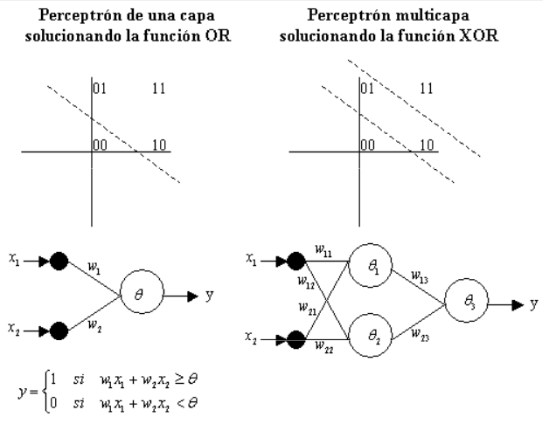
\includegraphics[width=0.8\textwidth]{images/ANN/2-ANN.png}
 \caption[Perceptrones solucionando la función OR y XOR.]{Perceptrones solucionando la función OR y XOR\cite{ANN_24}.\protect\footnotemark}
 \label{fig:ann_2}
\end{figure}
\footnotetext{Desde el punto de vista lógico la salida de la función OR es verdadera si algunos de los argumentos $x_1$ y $x_2$ son verdadero, y es falsa si todos los argumentos son falsos: entonces, la combinación $x_1=0$ y $x_2=0$ (en el gráfico de la izquierda representado por $00$) da una salida falsa; y las combinaciones $01$, $10$, $11$ verdadera. Lo que hacemos mediante el Perceptrón de una capa es separar estos resultados. En cambio, la salida de la función XOR es verdadera si las entradas no son iguales, y falso si son iguales; de esta manera $01$ y $10$ dan una salida verdadera, y $11$ y $00$ falsa. En este caso el Perceptrón multicapa puede separar estos dos resultados.}

Esta limitación al utilizar una única neurona es una de las principales razones por la cual surgió el esquema de Perceptrón multicapa, el cual se detalla en la siguiente sección.

\subsubsection{Perceptrón multicapa (MLP).}

El modelo de Perceptrón multicapa (MLP) es el modelo más conocido y utilizado de Redes Neuronales. Al igual que el modelo de Perceptrón Simple, MLP es un modelo de clasificación. Generalmente el modelo MLP se utiliza para describir el funcionamiento de una red neuronal, y es el esquema que utilizaremos para nuestra implementación del modelo Word2vec. En el modelo MLP la distribución de neuronas dentro de la red se realiza formando niveles o capas, con un número determinado de dichas neuronas en cada una de ellas. 

A continuación mencionaremos las tres capas existentes en el modelo MLP, cada una con distintas funciones.
\begin{itemize}
\item \textbf{Capa de entrada}: contiene las variables de entrada; reciben directamente la información proveniente de las fuentes externas de la red.
\item \textbf{Capas ocultas}: pueden haber 1 o N capa/s oculta/s. La longitud de N determina la profundidad de la red, dando origen al término de aprendizaje profundo (o \textit{deep learning}). Colocando neuronas en forma secuencial permite que cada neurona reciba información procesada por una neurona anterior, lo que significa que la red puede generar conocimiento jerarquizado: de esta manera la red podría aprender conocimiento básico en las primeras capas y mientras va pasando la información a las neuronas de las siguientes capas, va generando conocimiento más abstracto y complejo.
\item \textbf{Capa de salida}: permite retornar los resultados procesados por la red neuronal. Si estamos resolviendo un problema de clasificación esta capa puede estar formada por 2 neuronas (si se trata de una clasificación binaria) o N neuronas (en caso de clasificación multiclase). 
\end{itemize}

Cabe destacar que en nuestro modelo MLP, una única neurona de nuestra capa oculta o de nuestra capa de salida puede representarse como un Perceptrón Simple (Figura \ref{fig:ann_3}). En cambio, una neurona de nuestra capa de  entrada \textbf{no} puede representarse como un Perceptrón Simple, ya que en esta capa no existe ningún procesamiento interno. Con “procesamiento interno” nos referimos a la función de entrada y función de activación dentro de la neurona: por esta razón, las funciones de activación también residen únicamente en las neuronas de la capa oculta o en las neuronas de la capa de salida (las neuronas de la capa de entrada no poseen funciones de activación). 

\begin{figure}[H]    %[H] es para que se ubique justo debajo del texto anterior.
 \centering
 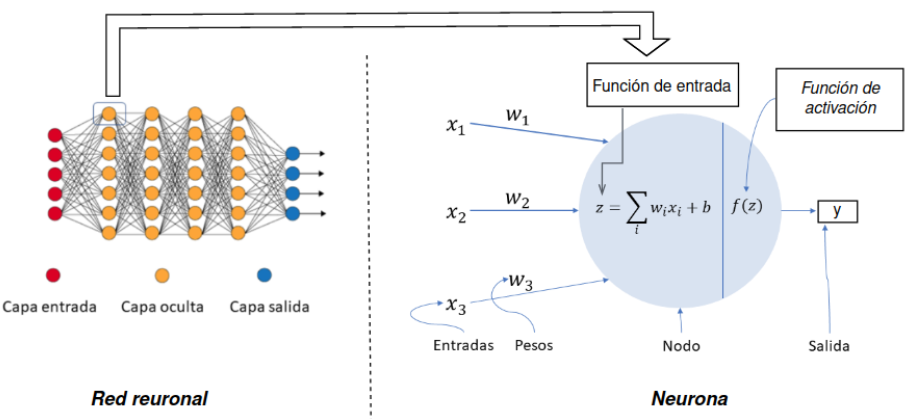
\includegraphics[width=1\textwidth]{images/ANN/3-ANN.png}
 \captionsetup{justification=centering,margin=3cm}
 \caption[Modelo Perceptrón Multicapa -MLP- (izquierda) y Perceptrón Simple (derecha).]{Modelo Perceptrón Multicapa -MLP- (izquierda) y Perceptrón Simple (derecha).}
 \label{fig:ann_3}
\end{figure}

Observando la parte izquierda de la Figura \ref{fig:ann_3}, podemos apreciar que cada una de las capas pueden estar compuesta por una o más neuronas, lo que significa que cada capa es un vector de neuronas. La dimensión del vector determina el ancho del modelo de una red neuronal. Cada capa recibe los datos de salida de la capa anterior. Luego, cada neurona de la capa actual realizará sus procesamientos en base a esta entrada (aplicando su función de entrada y función de activación), y su salida la pasará a cada neurona de la capa siguiente. Este tipo de redes se denominan \textit{feedforward}, debido a que el flujo de información va de una capa a la que sigue, sin bucles de retroalimentación. 

A continuación, explicaremos el modelo MLP desde un punto de vista matemático\cite{ANN_25}. Como mencionamos previamente, con el modelo de MLP es posible combinar varios perceptrones en una capa de procesamiento, con lo cual obtenemos una función $f:\mathbb{R}^m\rightarrow \mathbb{R}^n$ para cada capa (oculta o de salida), donde $m$ es el tamaño de la entrada, y $n$ es el número de perceptrones, que a su vez determinan el tamaño de la salida. De esta manera, dada una entrada $x$, la función $f$ procesa dicha entrada mediante la Formula \ref{eq:ecuacion_5_ANN}.

\begin{equation}\label{eq:ecuacion_5_ANN}
f(x) = \phi(Wx+b) \qquad  \text{(Ver \cite{ANN_25})}
\end{equation}

Donde $\phi$ es la función de activación que elegimos usar para esa capa, $W$ es la matriz de pesos, y $b$ es el vector que contiene los sesgos.

Además, como mencionamos previamente, con el modelo MLP podemos componer varias de estas capas, con lo cual obtenemos una \textit{red}, donde los perceptrones de una capa reciben como entrada a los de la capa anterior y alimentan a los de la capa que sigue. Dada una red $f$ y una entrada $x$, a la salida $f(x)$ se la denomina, naturalmente, capa de salida, mientras que a la entrada $x$ se la suele denominar capa de entrada. Cuando tenemos una red con varias capas, todas las capas que no son de salida ni de entrada se denominan capas ocultas. 

Anteriormente vimos que la red $f$ depende de los parámetros $W$ y $b$ (que en su conjunto vamos a denotar con $\theta$) y esta formada por una \textit{composición} sucesiva de varias capas $f^i$, donde el superíndice indica el número de la capa. De esta manera, cada capa cuenta con sus propios parámetros $\theta$ y procesa la información que recibe de acuerdo a la Fórmula \ref{eq:ecuacion_6_ANN}.

\begin{equation}\label{eq:ecuacion_6_ANN}
f^i(a^{i-1},\theta^i) = f^i(a^{i-1},w^i,b^i) = \phi(W^{i}a^{i-1}+b^i)    \qquad  \text{(Ver \cite{ANN_25})}
\end{equation}

Donde $a^{i-1}$ es la salida, o activación, de la capa anterior, $W^i$ es la matriz de pesos de la capa $i$ y $b^i$ es el vector de sesgos.

\subsubsection{Funciones de activación en MLP.}\label{Func_activ}

Como mencionamos previamente, las funciones de activación residen únicamente en las neuronas de la capa oculta o en las neuronas de la capa de salida (las neuronas de la capa de entrada no poseen funciones de activación).

Algo que vale la pena mencionar es que todas las capas ocultas suelen utilizar la misma función de activación. La capa de salida normalmente utiliza una función de activación diferente de las capas ocultas y depende del tipo de predicción requerida por el modelo.

El propósito de la función de activación es introducir una \textit{no-linealidad} dentro de la red neuronal, lo que le permite a la misma obtener una variable de salida $y$ que varíe de forma no lineal con respecto a sus variables de entrada $x$. A continuación explicaremos más en detalle \textit{¿por qué esta función de activación tiene que ser una función no lineal?}:
\begin{itemize}
\item Esto es debido a que si una red neuronal únicamente posee funciones de activación lineales (también conocidas como \textit{función identidad}), la red se comportará como si fuera un perceptrón de una sola capa: esto es debido a que si sumamos todas las capas obtendremos otra función lineal.
Independientemente de cuán compleja sea la arquitectura de la red, una función de activación lineal solo nos permite modelar una relación lineal entre las entradas y salidas, siendo efectiva solo en una capa de profundidad y para problemas de regresión lineal (por ejemplo al predecir precios de la vivienda), y no siendo útil para la mayoría de las aplicaciones del mundo real que son altamente no lineales.
Resumidamente, que la función de activación sea no lineal permite a la red apilar múltiples capas de neuronas para crear lo que se conoce como una red neuronal profunda, que se requiere para aprender conjuntos de datos complejos.
\end{itemize}

En nuestra implementación de red neuronal para el modelo Word2vec (ver sección \textit{\nameref{Implementacion_word_emb_y_wmd}}). no utilizamos funciones de activación en las neuronas de la capa oculta, este modelo \textit{únicamente utiliza la función de activación para la capa de salida}. 
El modelo Word2vec, en su esquema básico, utiliza una función de activación softmax para la capa de salida. En nuestra implementación se realizó una mejora a dicho esquema, introduciendo lo que se conoce como \textit{muestreo negativo} (el cual está explicado en la sección \textit{\nameref{neg_samp}}), que implementa una \textbf{función de activación sigmoide para la capa de salida}. En las siguientes secciones se detallarán dichas funciones de activación (softmax y sigmoide).

\paragraph{Softmax en la capa de salida.}\label{soft_capa_salida}

La función softmax comprime las salidas de cada neurona para que estas sean de 0 y 1 de tal forma que la suma de las salidas sea igual a 1. La función softmax produce salidas que se asemejan a probabilidades. Esto es, cada salida de la red produce una probabilidad entre 0 y 1, mientras que la suma de estas probabilidades es 1. Consecuentemente, esta función es usada en la capa de salida en ANN para resolver problemas de clasificación, ya que en estos problemas se requiere separar los datos de entrada en grupos. 
En la Fórmula \ref{eq:ecuacion_7_ANN} podemos observar la representación matemática de la función softmax; mientras que en la Figura \ref{fig:ann_4}. podemos observar la aplicación de esta función a la capa de salida de una red neuronal.

\begin{equation}\label{eq:ecuacion_7_ANN}
Z_k= \frac{e^{y_k}}{\sum_{k=1}^{M}e^{y_k}} \qquad \text{(Ver \cite{ANN_24})}
\end{equation}
\begin{center}
\textit{Función softmax.}
\end{center}

Donde $0 \geq Z_k \geq 1$, mientras que $y_k$ es la salida de la neurona $k$, la cual pasa a la función softmax para obtener la salida final $Z_k$, y $M$ es la cantidad total de neuronas en la capa de salida.     

\begin{figure}[H]    %[H] es para que se ubique justo debajo del texto anterior.
\centering
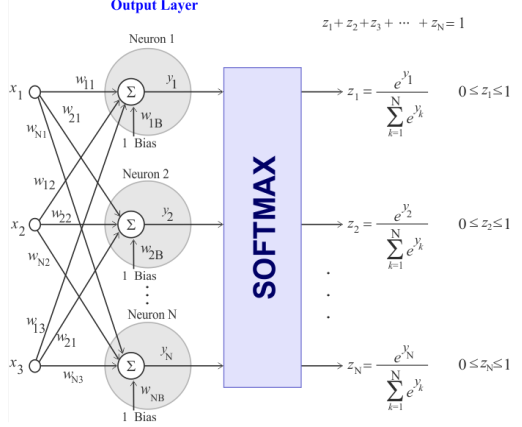
\includegraphics[width=0.8\textwidth]{images/ANN/4-ANN.png}
\caption[Función softmax aplicada a la capa de salida.]{Función softmax aplicada a la capa de salida\protect\footnotemark .}
 \label{fig:ann_4}
\end{figure}
\footnotetext{Obtenida del sitio web \url{http://sintesis.ugto.mx/WintemplaWeb}. (Consultado el 30 de abril de 2022).}

\paragraph{Sigmoide en la capa de salida.}\label{sigm_capa_salida}

La función sigmoide, o también llamada curva logística, es una aproximación suave de la función escalón. Como resultado de aplicar la función sigmoide a la salida $y_k$ de cada neurona, al igual que en la softmax, como salida obtenemos un valor $Z_k$ entre 0 y 1. Pero, a diferencia de la softmax, la suma de las salidas (de $Z_1$ a $Z_M$) no dan 1 como resultado, ya que en el denominador no se consideran a todas las salidas $y_K$ para realizar el cálculo de la función. 

Utilizando la función de activación sigmoide simplemente se aplica una función $\sigma(y_k)$ por cada $y_k$ salida de la respectiva neurona. Matemáticamente podemos observar la función sigmoide en la Fórmula \ref{eq:ecuacion_8_ANN}. 
Mientras que en la Figura \ref{fig:ann_5} podemos observar la representación gráfica de la función sigmoide comparándola, por ejemplo, con la función escalón. 

\begin{equation}\label{eq:ecuacion_8_ANN}
\sigma(y_k)= \frac{exp(y_k)}{ {1 + exp(y_k)}} =  \frac{1}{ {1+exp(-y_k)}}    \qquad \text{(Ver \cite{ANN_25})}
\end{equation}
\begin{center}
\textit{Función sigmoide.}
\end{center}

Donde $0 \geq \sigma(y_k) \geq 1$.    

\begin{figure}[H]    %[H] es para que se ubique justo debajo del texto anterior.
 \centering
 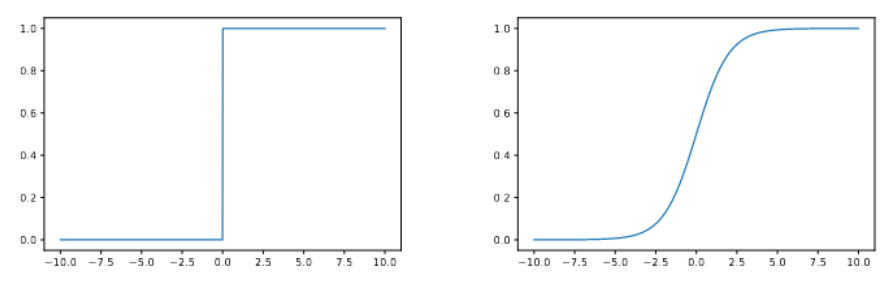
\includegraphics[width=1\textwidth]{images/ANN/5-ANN.png}
 \caption{Funciones de activación escalón y sigmoide\cite{ANN_25}.} 
 \label{fig:ann_5}
\end{figure}

\subsubsection{Entrenamiento en una red neuronal.}\label{entren_ann}

Como se comentó anteriormente, el modelo MLP de Redes Neuronales es un modelo de clasificación, lo que significa que realiza un aprendizaje supervisado. De esta manera, a la red neuronal durante el proceso de entrenamiento se le muestra un gran número de datos de entrenamiento para que la red ajuste / modifique sus pesos de manera iterativa y de este modo, lograr minimizar el error producido en la respuesta: lograr minimizar la \textit{función de costo}, la cual penaliza de alguna manera los errores que comete la red al clasificar. Luego de varias iteraciones de ejemplos, se espera que la red neuronal sea efectiva para resolver la tarea para la que fue entrenada.
En otras palabras, una red aprende resolviendo un problema de optimización, donde se buscan los parámetros de la red (pesos y sesgos, $\theta$) que minimizan la función de costo o error $J$ para cada ejemplo $x_i$ en el conjunto de entrenamiento $X$. 

A continuación describiremos en mayor detalle el ciclo iterativo de procesos del entrenamiento de una red neuronal\cite{ANN_25}.

\begin{enumerate}
\item Al comienzo del algoritmo, por única vez, se inicializan las matrices de pesos $W$ y los vectores de bias $b$ de toda la red con valores aleatorios. Estos son los \textit{parámetros} $\theta$ de nuestro modelo de red neuronal.
  
\item Se aplica \textit{forward propagation} (o propagación hacia adelante) para cada una de las muestras del set de entrenamiento y se obtienen los puntajes de salida $y$. Forward propagation es la manera en que una ANN computa los valores de entrada y los clasifica. Matemáticamente, durante este proceso la red neuronal recibe un vector de entrada $x$ y devuelve un vector de salida $y$\footnote{Cada elemento del vector de salida $y$ se corresponde a la salida de una $k$ neurona de la capa de salida.} aplicando en cada una de las capas de la red $f^{i}$ la Fórmula \ref{eq:ecuacion_6_ANN} (que alimentará a la capa $f^{i+1}$, y que generalmente involucra sumatoria, multiplicación y uso de funciones de activación). De esta manera la señal se mueve desde la capa de entrada, pasando por las capas ocultas intermedias, hasta llegar a la capa de salida con algún valor.

\item Los vectores de salida $y$ obtenidos / predichos de todas las muestras de entrenamiento se comparan con los valores de sus vectores de salida $y'$ correspondientes que tiene las etiquetas reales, computándose de esta manera el \textit{error} (o \textit{loss}) de clasificación (entre el valor predicho y el real) mediante el cálculo de la \textit{función de costo / pérdida (loss function)}.

La función de pérdida $J(\theta)$ será diferente para cada modelo. Más adelante obtendremos los cálculos de las $J(\theta)$ que tendremos en consideración para nuestra implementación: Fórmulas \ref{eq:ecuacion_11_NLP} y \ref{eq:ecuacion_21_NLP}, siendo esta última la que finalmente utilizaremos en nuestro modelo y buscaremos minimizar. Ambas funciones de costo son la sumatoria sobre los costos individuales en los que incurre la red al clasificar cada elemento del conjunto de entrenamiento, y se calculan 1 vez por epoch\footnote{Epoch es un hiper-parámetro de nuestra red neuronal, donde cada epoch representa una iteración sobre nuestros datos de entrenamiento completo. Esta iteración incluye el cálculo de los forward propagation y back propagation correspondientes.}.

\item Se aplica el proceso conocido como \textit{backpropagation} (o propagación hacia atrás). No se explicará en detalle este procedimiento porque no entra dentro de los objetivos de este trabajo. Lo que hay que tener en cuenta es que backpropagation utiliza la función de optimización\footnote{Una función de optimización en redes neuronales tiene como objetivo encontrar los pesos W que minimicen los errores de clasificación / la función de coste.} \textit{descenso del gradiente} para poder ajustar / modificar los pesos y el bias de cada neurona de nuestra red \textit{con el objetivo de minimizar la función de costo $J(\theta)$ obtenida en el paso 3}, y con ello minimizar el error de clasificación. En backpropagation calculamos el gradiente de $J(\theta)$ (o dicho de otra forma derivamos el error) en función de cada uno de los parámetros de nuestra red. Para esto se opera recursivamente capa tras capa propagando el error desde la salida hacia la entrada de la red.

De esta manera, considerando que nuestra función de pérdida es $J(\theta)$, donde nuestros parámetros $\theta$ son $W$ (matriz de pesos) y $b$ (vector de bias), el objetivo de nuestro modelo será encontrar los valores óptimos de $W$ y $b$ ($\theta^{(new)}$) para minimizar $J(\theta)$. De esta manera, en la Fórmula \ref{eq:ecuacion_9_ANN} podemos observar la ecuación general de actualización de nuestros parámetros $\theta$ para la red reuronal.
 
\begin{equation}\label{eq:ecuacion_9_ANN}
\theta^{(new)} = \theta^{(old)} - n \cdot \nabla J(\theta)   \qquad \text{(Ver \cite{ANN_25})}
\end{equation}
\begin{center}
\textit{Fórmula de actualización de parámetros de nuestra ANN.}
\end{center}

Donde $n$ es la tasa de aprendizaje (o learning rate), del cual hablaremos con mayor detalle en la sección \textit{\nameref{hiper_n}}, y $\nabla J(\theta)$ es el gradiente (también llamado pendiente o derivada) de la función $J(\theta)$ para nuestros parámetros $\theta^{(old)}$. Al tener un “-” por delante obtenemos el gradiente negativo, el cual apunta en la dirección de máximo decrecimiento de la función. Este gradiente negativo permite “guiar” al algoritmo descenso del gradiente para acercarse, de manera progresiva debido a $n$, al mínimo ideal de la función.      

\item Volver al paso 2 hasta completar la cantidad de epochs seteados como hiper-parámetro de nuestro modelo de red neuronal. 

\end{enumerate}

Cabe destacar que este entrenamiento descrito tiene en cuenta el uso del \textit{algoritmo de gradiente descendiente “básico”} y no el \textit{algoritmo de gradiente descendiente estocástico} (stochastic gradient descent, \textit{SDG}), algo que explicaremos en mayor detalle en la sección \textit{\nameref{ent_costo_softmax}}.

\paragraph{Hiper-parámetro n.}\label{hiper_n}

Como detallamos anteriormente, $n$ es la tasa de aprendizaje de nuestra red neuronal e interviene en la actualización de nuestros parámetros  $\theta$ al aplicar backpropagation utilizando el algoritmo descenso del gradiente. $n$ define y permite regular la velocidad con la que nos desplazamos por el espacio de parámetros y por lo tanto cuán rápido nos acercamos al mínimo de la función $J(\theta)$. $n$ definirá la cantidad de iteraciones requerida para que el algoritmo descenso del gradiente encuentre el mínimo de la función.

A diferencia de $\theta$, $n$ es un parámetro que no es ajustado por el algoritmo de optimización del descenso del gradiente, sino que debe ser configurado por separado. Como mencionamos anteriormente, a este tipo de parámetros se los denomina hiper-parámetros, y requieren de cierto cuidado en su elección para garantizar el buen rendimiento de la red neuronal. 

Mientras más rápido nos acerquemos al mínimo de la función, más rápido la red estará aprendiendo a realizar su tarea. Sin embargo, como ya mencionamos antes, valores muy altos del hiper-parámetro $n$ pueden tener un efecto contrario, llevando a que eventualmente el algoritmo pase de largo de manera reiterada este mínimo, impidiendo el aprendizaje. A veces aprender requiere ir más lento y ser más cuidadosos. Lo mismo ocurre con la red, y en ese caso es conveniente ajustar $n$ para conseguir que la red no pase por alto los detalles. En la Figura \ref{fig:ann_6} podemos observar el efecto de diferentes tasas de aprendizaje durante el entrenamiento. 

\begin{figure}[H]    %[H] es para que se ubique justo debajo del texto anterior.
 \centering
 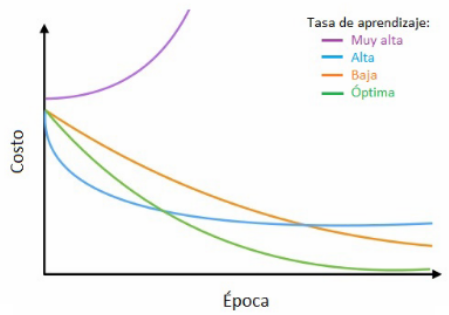
\includegraphics[width=0.5\textwidth]{images/ANN/6-ANN.png}
  \captionsetup{justification=centering,margin=3cm}
 \caption{Efecto de diferentes tasas de aprendizaje $n$ durante el entrenamiento\cite{ANN_25}.} 
 \label{fig:ann_6}
\end{figure}

Una tasa de aprendizaje demasiado alta puede ocasionar que el algoritmo de entrenamiento no pueda disminuir el costo de entrenamiento más allá de cierto punto, o en el peor de los casos puede ocasionar que el mismo aumente. Una tasa de aprendizaje demasiado baja puede hacer que el costo disminuya muy lentamente, ralentizando el aprendizaje. La tasa de aprendizaje $n$ ideal es un compromiso entre lograr una disminución significativa del costo y mantener una buena velocidad de aprendizaje\cite{ANN_25}.
\cleardoublepage

\section{Natural Language Processing.}\label{4.NaturalLanguageProcessing}

\subsection{Introducción.}\label{Intro_NLP}

El Procesamiento del Lenguaje Natural o Natural Language Processing (NLP) es un subconjunto de la Inteligencia Artificial (IA) que tiene como objetivo principal la construcción de sistemas que permitan procesar el lenguaje humano capturando la complejidad del mismo, y traducirla en información resumida produciendo \textit{resultados} comprensibles por la computadora o \textit{respuestas} comprensibles por humanos como parte de la aplicación/implementación de IA. De esta manera, NLP permite que las computadoras puedan \textit{comprender} el lenguaje humano.

Para abordar este problema y poder extraer el significado de los lenguajes humanos, la mayoría de las técnicas de NLP se basan y utilizan enfoques del aprendizaje automático (machine learning) y del aprendizaje profundo (deep learning)\cite{NLP_1, NLP_2}.

NLP podría definirse como ``la disciplina que estudia los aspectos lingüísticos de la comunicación humano-humano y humano-máquina, desarrolla modelos de competencia y desempeño lingüísticos, emplea marcos computacionales para implementar procesos que incorporan tales modelos, identifica metodologías para el refinamiento iterativo de tales procesos/modelos e investiga técnicas para evaluar los sistemas resultantes''\cite{NLP_3_4}.

NLP es un área interdisciplinaria basada en muchos campos de estudio. Estos campos incluyen a la informática, que proporciona técnicas para la representación de modelos y el diseño e implementación de algoritmos; la linguística, que identifica modelos y procesos linguísticos; las matemáticas, que aporta modelos y métodos formales; la psicología, que estudia modelos y teorías del comportamiento humano; la filosofía, que proporciona teorías y preguntas sobre los principios subyacentes del pensamiento, el conocimiento linguístico y los fenómenos; estadísticas, que proporciona técnicas para predecir eventos basados en datos de muestra; ingeniería eléctrica, que aporta teoría de la información y técnicas para el procesamiento de señales; y biología, que explora la arquitectura subyacente de los procesos linguísticos en el cerebro\cite{NLP_3_4}.

\cleardoublepage

\subsection{Aplicaciones NLP.}\label{Aplicaciones_NLP}

Como mencionamos previamente, NLP generalmente utiliza algoritmos de machine learning y deep learning para resolver distintos problemas. Algunas de las áreas más interesantes donde se aplica NLP junto con ML y/o DL para la resolución de problemas son\cite{NLP_5, NLP_6}:

\begin{itemize}
\item \textbf{Traducción automática (Machine Translation, MT)}. Estas aplicaciones implican el uso de técnicas matemáticas y algorítmicas para traducir documentos de un idioma humano a otro. Realizar una traducción eficaz es muy complicado incluso para los seres humanos, ya que requiere de gran comprensión y conocimiento de las palabras, frases, sensibilidades culturales, sintaxis y la semántica de los dos idiomas involucrados. 

\item \textbf{Resumidores de texto (Text Summarization)}. Estas aplicaciones permiten encontrar elementos de interés en los documentos para producir un resumen del contenido más importante. Estas tareas incluyen procesamiento de texto sintáctico, semántico y del nivel de voz. Hay dos tipos principales de resumen: extractivo y abstractivo. El primero se enfoca en la extracción, simplificación, reordenación y concatenación de oraciones para transmitir la información importante en los documentos usando texto tomado directamente de los documentos. En cambio, los resúmenes abstractivos se basan en expresar el contenido de los documentos a través de la abstracción de estilo generacional, posiblemente usando palabras nunca vistas en los documentos.

\item \textbf{Generación de texto (Text Generation)}. Muchas tareas de NLP requieren la generación de un lenguaje similar al humano. Las aplicaciones de \textit{Text Summarization} y \textit{Machine Translation} convierten un texto en otro de secuencia a secuencia (seq2seq). Otras tareas, como los subtítulos de imágenes y videos y los informes meteorológicos y deportivos automáticos, convierten datos no textuales en texto. Algunas tareas, sin embargo, producen texto sin datos de entrada para convertir (o con solo pequeñas cantidades utilizadas como guía). Estas tareas incluyen la generación de poesía, la generación de chistes y la generación de historias.

\item \textbf{Clasificación de texto (Text Classification)}. Text Classification permite la asignación de documentos de texto a clases predefinidas (pueden tratarse de muchas clases o simplemente de una clasificación binaria). Una de las aplicaciones más populares de Text Classification es el \textit{análisis de sentimiento (Sentiment Analysis)}. Un ejemplo de una tarea de Sentiment Analysis es la extracción del sentimiento de un escritor y su clasificación: si su inclinación fue positiva, negativa o neutral hacia algún tema o idea.

\item \textbf{Sistemas de recuperación de información (Information Retrieval -IR- systems)}. El propósito de los sistemas IR es ayudar al usuario a encontrar la información correcta (más útil) en el formato correcto (más conveniente) en el momento correcto (cuando la necesiten). Esta información se encuentra en documentos digitales; y lo que se intenta recuperar son textos, imágenes, sonidos o datos de otras características que sean relevantes para el usuario. Entre muchos problemas en IR, un problema principal que debe abordarse se relaciona con la clasificación de documentos con respecto a una cadena de consulta en términos de puntajes de relevancia para tareas de recuperación ad-hoc, similar a lo que sucede en un motor de búsqueda. Los modelos de DL sirven para resolver estos problemas, permitiendo para la recuperación ad-hoc hacer coincidir los textos de las consultas con los textos de los documentos para obtener puntajes de relevancia.

\item \textbf{Sistemas de extracción de información (Information Extraction -IE- systems)}. El propósito de los sistemas IE es extraer información explícita o implícita del texto. Los resultados de los sistemas varían, pero a menudo los datos extraídos y las relaciones dentro de ellos se guardan en bases de datos relacionales. La información comúnmente extraída incluye entidades, relaciones o eventos en el texto. 

\begin{enumerate}
\item \textit{Named Entity Recognition (NER)}: Se refiera a identificar y reconocer entidades en los textos y “tagearlas”: por ejemplo personas, empresas, fechas, lugares, precios, etc.
\item \textit{Extracción de eventos}: Se ocupa de identificar palabras o frases que se mencionan o refieren a la ocurrencia de eventos junto con los participantes, roles de los mismos, objetos, momentos en que dicho evento ocurrió y desencadenantes del mismo.
\item \textit{Extracción de relaciones}: Implica la extracción de relaciones en los textos, las cuales pueden ser relaciones posesivas, antónimas o sinónimas, familiares o geográficas.
\end{enumerate}

\item \textbf{Respuestas a preguntas (Question Answering, QA)}. Al igual que las aplicaciones de Text Summarization e IE, los sistemas de QA recopilan palabras, frases u oraciones relevantes de un documento. QA devuelve esta información de manera coherente como respuesta a una solicitud o consulta de un usuario. Dada una pregunta y un conjunto de documentos, un sistema de QA intentará encontrar la respuesta exacta, o al menos la parte exacta del texto en la que aparece la respuesta.

\item \textbf{Reconocimiento de voz (Speech Recognition)}. Speech Recognition es el proceso de asignar señales de voz acústicas a un conjunto de palabras. Las dificultades de esta tarea surgen debido a las amplias variaciones en la pronunciación de las palabras y las ambigüedades homónimas y acústicas.

\item \textbf{Combinación de voz (Speech Combination)}. Speech Combination permite la producción o creación de expresiones de oraciones en lenguaje natural. Para poder crear expresiones el texto debe procesarse, por lo tanto NLP es un componente esencial para estos sistemas.

\item \textbf{Sistemas de intercambio (Exchange Systems)}. Por lo general estos sistemas se enfocan en una aplicación de caracterización limitada (por ejemplo, una heladera o sistema de sonido doméstico) y utilizan los niveles fonéticos y léxicos del idioma. 

\item \textbf{Imitación de autores (Author mimicking)}. Teniendo suficientes datos se pueden utilizar modelos de DL para generar textos que repliquen el estilo particular de un escritor.
\end{itemize}

\cleardoublepage

\subsection{NLP en la práctica.}\label{Practica_NLP}

En la práctica, NLP se utiliza como \textit{complemento} junto a algoritmos de ML o DL para realizar distintas tareas, las cuales pueden ser por ejemplo las mencionadas en la sección  \textit{\nameref{Aplicaciones_NLP}}.

Para la implementación de este Proyecto, la \textit{tarea específica} que involucra el uso de técnicas de NLP es la obtención de mediciones de similitud entre dos textos, las cuales posteriormente serán utilizadas como entradas a algoritmos de ML (en nuestro caso K-means, y luego KNN) para realizar la \textit{tarea global} de clasificación de nuestro Proyecto: en base a dichas mediciones de similitud lograr clasificar qué tan similares son los curriculums vitae de nuevos candidatos con respecto a la descripción de un puesto de IT.

La obtención de estas mediciones de similitud, resumidamente, involucra dos pasos\cite{Similarity_calculation}:
\begin{enumerate}
\item Convertir cada uno de los documentos de texto en un objeto matemático (vector numérico).
\item Definir y emplear una métrica de distancia que será utilizada como nuestra medida de similitud entre los vectores numéricos obtenidos del paso anterior, los cuales representan nuestros textos.
\end{enumerate}

Sin embargo, anteriormente al primer paso, y en general para cualquier tipo de tarea de NLP que implica manipulación de datos de texto, nuestros textos deben \textit{pre-procesarse} para lograr una limpieza y normalización de los mismos de modo que posteriormente puedan ser convertidos en vectores numéricos\cite{NLP_2}.

A modo de resumen, en la Figura \ref{fig:Imagen_NLP_1} se describen los pasos generales necesarios para obtener finalmente una representación vectorial de nuestros documentos de texto y posteriormente aplicar las mediciones de similitud sobre los mismos.

\begin{figure}[H]    %[H] es para que se ubique justo debajo del texto anterior.
 \centering
 \noindent\makebox[\textwidth]{%
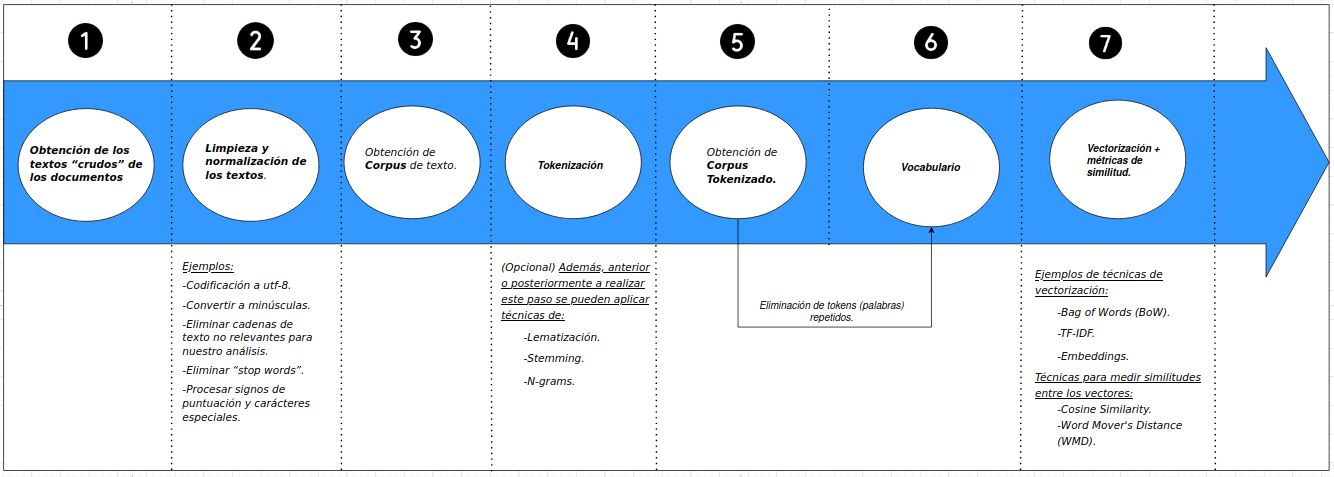
\includegraphics[width=1.2\textwidth]{images/NLP/1.png}}
 \caption{Pasos generales de nuestro proceso NLP.}
 \label{fig:Imagen_NLP_1}
\end{figure}

\cleardoublepage

El primer paso, que consiste en la obtención de los textos “crudos” de los documentos que utilizaremos en los sub-siguientes pasos, será explicado directamente en la sección de implementación, donde se obtienen los textos de los Curriculum Vitae y de las descripciones de puestos laborales de IT (Ver sección \textit{\nameref{obtencion_set_datos}}). Mientras que los pasos 2-7 serán explicados en detalle en las secciones posteriores. 

Algo a tener en cuenta es la diferencia entre \textit{corpus tokenizado} y \textit{vocabulario} (pasos 5 y 6 de la Figura \ref{fig:Imagen_NLP_1}), debido a que mencionaremos estos conceptos muy a menudo. El \textit{corpus tokenizado} son todas las palabras de nuestro corpus -el cual fue previamente tokenizado-, mientras que el \textit{vocabulario} es el set de palabras \textit{únicas} -sin repetir- obtenidas de dicho \textit{corpus tokenizado}.

Para entender mejor esto, detallaremos un ejemplo pasando por todas las fases descritas en la Figura  \ref{fig:Imagen_NLP_1}. Partiendo de “She will park the car on the street so we can walk in the central park” como nuestro texto “crudo” de documento, pasamos a la segunda fase de \textit{limpieza y normalización} (donde, entre otras cosas, se eliminan las stop words). De esta manera nos quedaría el \textit{corpus}: “park car street walk central park”. Este corpus pasa luego por la fase de \textit{tokenización}, en la cual se particiona el texto en pequeñas partes llamadas “tokens”. Estos tokens se agrupan formando el \textit{corpus tokenizado}, el cual será un vector [“park”, “car”, “street”, “walk”, “central”, “park”] con un tamaño de 6. Por último, para formar nuestro \textit{vocabulario} simplemente eliminamos los tokens (o palabras) repetidos, quedándonos el vector [“park”, “car”, “street”, “walk”, “central”] de tamaño 5. 
\\

\subsection{Preprocesamiento de textos.}\label{Proces_textos}

Este paso consiste en limpiar y normalizar nuestros textos de modo que posteriormente puedan ser convertidos en vectores numéricos. El pre-procesamiento de datos usualmente tiene un impacto significativo en la performance de generalización de nuestro algoritmo de machine learning\cite{preprocessing}.

Algunas palabras no son útiles en términos de poder predictivo porque son demasiado frecuentes y, por lo tanto, poco discriminantes. El objetivo del pre-procesamiento es preparar la representación de nuestros textos para que puedan alimentar a nuestros modelos de ML.

Las tareas de pre-procesamiento de textos más esenciales incluyen eliminar carácteres especiales o carácteres específicos que no son relevantes para nuestros análisis, convertir a minúscula nuestros textos, remover las ‘stopwords’, aplicar stemming y/o lemmatization, tokenizar nuestros textos, usar n-gramas, etc. A continuación explicaremos en mayor detalle estas tareas\cite{NLP_2}.

\cleardoublepage

\subsubsection{Limpieza y normalización.}\label{Limpieza_y_norm}

En esta limpieza inicial podemos considerar las siguientes sub-tareas:
\begin{enumerate}

\item \textit{Codificar nuestros textos a utf-8}: es común enfrentar problemas de representación y codificación cuando nuestros textos tienen algunos carácteres específicos, como por ejemplo acentos. Para evitar estos tipos de problemas generalmente se aplica una codificación a UTF-8 antes de procesar los textos.
\item \textit{Convertir nuestros textos a minúsculas}: Pasar cada letra de nuestros textos a minúsculas permitirá eliminar cualquier ambigüedad entre letras minúsculas y mayúsculas. 
\item \textit{Eliminar palabras o cadenas de texto no relevantes}: Por ejemplo, podemos eliminar e-mails, páginas web o palabras que no necesitemos tener en cuenta en nuestros análisis. Para eliminar e-mails o páginas web podemos utilizar \textit{expresiones regulares}\footnote{Las expresiones regulares nos permiten identificar patrones y aplicar reglas cuando estos se detectan. De esta manera, podemos extraer información textual que sigue un formato particular: por ejemplo, “Mr /. (. *)” es una expresión regular que permite buscar los textos que empiecen con ‘Mr’ y tener en cuenta el grupo que le sigue, el cual se supone que representa el nombre de la persona\cite{NLP_2}.}, las cuales nos ayudan a identificar los formatos de URLs o casillas de mail y aplicar algún tipo de regla para eliminarlos (reemplazandolos por palabras vacías). 
\item \textit{Procesar signos de puntuación y carácteres especiales}: Esta tarea no precisamente consiste en eliminar los signos de puntuación y carácteres especiales, ya que si bien algunos de ellos no son necesarios, otros sí lo son. Por ejemplo, en tareas de análisis de sentimiento, un signo de exclamación en un tweet puede expresar un énfasis en su sentimiento, ya que las personas tienden a aumentar el número de signos de exclamación cuando se trata de sentimientos fuertes. Por lo tanto, los carácteres especiales y de puntuación pueden conservarse o eliminarse (reemplazandolos por palabras vacías). Estas palabras con signos de puntuación y/o carácteres especiales, también pueden tratarse utilizando expresiones regulares.
\item \textit{Eliminación de “stop words”}:  Los humanos al comunicarnos usamos palabras como “el”, “y” o “a” para que las oraciones tengan sentido. Sin embargo, estas palabras no tienen ningún significado y no son útiles para el análisis de datos. Las “stop words” se consideran palabras vacías y deshacerse de las mismas es un paso del pre-procesamiento que permite centrarse en las palabras que importan. Cada idioma posee su propia lista de palabras vacías que se pueden ajustar según el problema. 

\end{enumerate}

\cleardoublepage

\subsubsection{Tokenización.}\label{tokenizacion}

Como explicamos previamente, los textos necesitan ser tratados previamente a ser convertidos en números y ser procesados por un modelo. Para lograr esto, luego de realizar las tareas de limpieza inicial detalladas en la sección anterior, se debe tokenizar (o particionar) los textos. 

La \textit{tokenización} consiste en dividir un texto en partes más pequeñas llamadas \textit{tokens} y luego re-agrupar los mismos formando una lista de tokens. Un token puede ser un párrafo del texto, una oración, una palabra o cada uno de los carácteres de nuestro texto. Generalmente se arman los tokens dividiendo al texto en palabras. En la Figura \ref{fig:Imagen_NLP_2} podemos observar una tokenización a nivel de palabras, mientras que en la Figura \ref{fig:Imagen_NLP_3} se realiza a nivel de carácteres. 

\begin{figure}[H]    
 \centering
 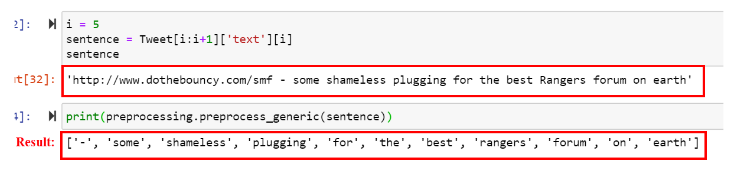
\includegraphics[width=1\textwidth]{images/NLP/2.png}
 \caption{Tokenización por palabras\cite{NLP_2}.}
 \label{fig:Imagen_NLP_2}
\end{figure}

\begin{figure}[H]    
 \centering
 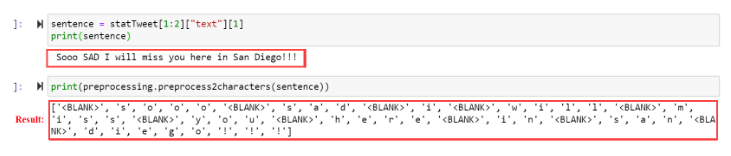
\includegraphics[width=1\textwidth]{images/NLP/3.png}
 \caption{Tokenización por carácteres\cite{NLP_2}.}
 \label{fig:Imagen_NLP_3}
\end{figure}

Tokenizar las palabras nos permite encontrar similitudes entre las mismas: por ejemplo, detectar las palabras con las mismas raíces. Para encontrar estas similitudes podemos utilizar los métodos de \textit{stemming} y \textit{lemmatization}, los cuales se verán en la próxima sección.

La lista de tokens que obtendremos luego de aplicar tokenización (y en caso de ser necesario stemming, lemmatization y N-grams) sobre todos los documentos de texto incluidos en nuestros datos, es el \textit{corpus tokenizado} que mencionamos previamente. Luego, al eliminar los tokens repetidos, podemos obtener nuestro \textit{vocabulario}, el cual será útil en tareas posteriores.

\cleardoublepage

\subsubsection{Stemming y lemmatization.}\label{stem_y_lem}

Como mencionamos previamente, estas dos técnicas nos permiten encontrar similitudes entre las palabras, y por ejemplo, detectar las palabras con las mismas raíces.

\begin{itemize}

\item \textit{Stemming (derivación)}: Las reglas gramaticales a menudo exigen que se agreguen algunos sufijos a las palabras para que una oración tenga sentido; sin embargo, estos sufijos no son imperativos cuando se trata de comprender el significado de una palabra. Stemming es un paso del pre-procesamiento que elimina las partes innecesarias de una palabra manteniendo su \textit{raíz} (“\textit{root}” o también llamado “\textit{stem}” en inglés). Podemos ver un ejemplo de stemming en la Figura \ref{fig:Imagen_NLP_4}.

\begin{figure}[H]    
 \centering
 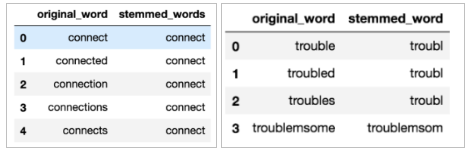
\includegraphics[width=0.7\textwidth]{images/NLP/4.png}
 \caption{Stemming\cite{NLP_2}.}
 \label{fig:Imagen_NLP_4}
\end{figure}

\item \textit{Lemmatization (lematización)}: Mientras que stemming elimina los sufijos y prefijos de una palabra y solo mantiene su raíz, lemmatization es un algoritmo que reemplaza una palabra por su forma más básica, también llamada “lema”. Un lema puede ser una forma infinitiva, un sustantivo, un adjetivo, etc., mientras que una raíz a menudo no significa nada: podemos ver por ejemplo en la Figura \ref{fig:Imagen_NLP_4} que el stem ‘troublemsom’ no tiene ningún significado. 

Utilizar lemmatization es útil porque en algunos idiomas, las palabras con diferentes significados pueden tener la misma raíz, y utilizando stemming nos daría la misma raíz para todas las palabras, lo que supondría algo incorrecto. Por lo tanto, los lemas tienen como objetivo transmitir una idea con una palabra real en lugar de una raíz básica sin un significado definido, corrigiendo el problema de tener dos conceptos diferentes con la misma raíz. Por lo tanto, la lematización requiere un análisis morfológico de la palabra y la existencia de un diccionario detallado para que funcione el algoritmo, lo que hace que su implementación sea más compleja que utilizar stemming. Podemos ver un ejemplo de lemmatization en la Figura \ref{fig:Imagen_NLP_5}.

\begin{figure}[H]    
 \centering
 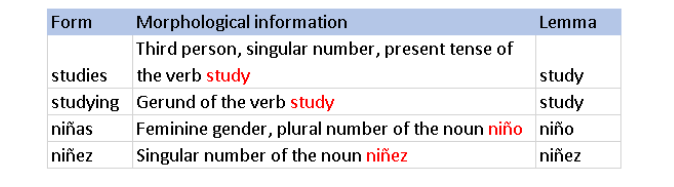
\includegraphics[width=0.7\textwidth]{images/NLP/5.png}
 \caption{Lemmatization\cite{NLP_2}.}
 \label{fig:Imagen_NLP_5}
\end{figure}

\end{itemize}

\cleardoublepage

\subsubsection{N-grams.}\label{ngrams}

A veces, asociar / juntar palabras puede cambiar el significado o traer información diferente. Por ejemplo, si estamos prediciendo el sentimiento de una oración, se esperaría que la palabra ``malo'' empujara la salida de un modelo hacia una etiqueta negativa. Sin embargo, ``no está mal'' haría lo contrario. Debido a esto, es posible que debamos considerar ``no está mal'' como una palabra única. 

La construcción de nuevas ``palabras'' provenientes de la co-ocurrencia de palabras se llama ``n-grams'', donde ``n'' representa el número de palabras que nos gustaría considerar (en nuestro ejemplo ``no está mal'' es un ``3-grams''). Este procesamiento tiene como objetivo enriquecer el diccionario de palabras\cite{NLP_2}.
\\

\subsection{Obtención de representaciones vectoriales.}\label{rep_vect}

Una vez que nuestros datos están limpios y ya tenemos nuestro \textit{corpus tokenizado} (formado por tokens de palabras de nuestros textos), el siguiente paso es transformar estos datos \textit{textuales} en representaciones vectoriales \textit{numéricas} mediante \textbf{técnicas de vectorización}.

Esta operación se lleva a cabo debido a que las computadoras y los algoritmos de machine learning no pueden entender ni aprender utilizando textos o palabras, ya que operan en un espacio de valores numéricos. Por lo tanto, para realizar tareas de ML sobre textos, necesitamos transformar nuestros documentos en representaciones vectoriales con valores numéricos. El objetivo es que la representación vectorial de nuestros documentos \textit{representen nuestro lenguaje de la mejor forma posible para que los modelos de ML usados posteriormente puedan aprender los patrones necesarios para entender dicho lenguaje}\cite{NLP_7}.

Existen distintas técnicas de vectorización para lograr esto. A continuación se detallarán algunas de las más populares y utilizadas\cite{NLP_2}.

\cleardoublepage

\subsubsection{Bag of Words (BoW).}\label{bow}

\textit{Bag of Words (BoW)}, o también llamado ‘Count Vector’, es el método fundamental y más básico para obtener nuestras representaciones vectoriales de documentos. Suponiendo que tenemos $N$ documentos de texto, el modelo BoW permite representar cada uno de estos documentos como una bolsa, la cual contiene algunas palabras. Estas palabras se encuentran dentro de un \textit{diccionario} de palabras. De esta manera, BoW mediante un modelado basado en diccionarios, \textit{describe la frecuencia u ocurrencia de cada una de las palabras en los documentos}.

El primer paso del método BoW consiste en crear dicho diccionario (al que representaremos como $D$), el cual contiene nuestro \textit{vocabulario}. Este vocabulario representa a todas las palabras (sin repetir) de nuestro conjunto de documentos de texto $d$.

Luego, suponiendo que nuestro conjunto de documentos $d$  está formado por $n$ documentos, y queremos obtener una representación vectorial para cada una de los $d[N]$ documentos, lo que se hace es utilizar el diccionario $D$ obtenido del paso anterior para generar una matriz que cuente la cantidad de veces que aparece cada una de las palabra únicas de $d$ para cada uno de nuestros $d[N]$ documentos.

En la Fórmula \ref{eq:ecuacion_1_NLP} podemos observar la representación matemática de nuestro set de documentos  $d$.

\begin{equation}\label{eq:ecuacion_1_NLP}
d = (w_i),      \text{    para  } i\in[1,n_d] 
\end{equation}

Donde:
\begin{itemize}
\item $w$ es un \textit{segmento} formado por una secuencia finita de \textit{caracteres}. Si nuestros \textit{caracteres} son letras, un \textit{segmento} podría ser una palabra.
\item $d \in D$, siendo $D$ nuestro diccionario de secuencias finitas de segmentos $w$ sin repetir (o vocabulario). 
\item $n_d$ es la longitud de $d$ (número total de palabras del set de documentos).
\end{itemize}

Resumidamente, $d$ es un conjunto de segmentos $w_i$, y $D$ está compuesto por un conjunto de segmentos $w_i$ sin repetir (nuestro vocabulario).

\cleardoublepage

Como mencionamos previamente, la representación vectorial mediante BoW indica la cantidad de veces que aparece cada palabra en nuestro corpus. Cada componente del vector indica esta cantidad. En el ejemplo de la Tabla \ref{table:bow_1}, cada columna representa las palabras que componen nuestro vocabulario / diccionario $D$, y cada fila indica la representación vectorial mediante BoW para cada documento (sin realizar un pre-procesamiento).

\begin{table}[h!]
\centering
\begin{tabular}{|p{4cm}||p{1cm}|p{1cm}|p{1cm}|p{1cm}|p{1cm}|p{1cm}|p{1cm}|p{1cm}|}
\hline
\textbf{Vocabulario$\Rightarrow$ Corpus $\Downarrow$} & the & cat & sat & on & hat & dog & ate & and \\ [1ex] 
\hline
\textit{The cat sat on the hat} & 2 & 1 & 1 & 1 & 1 & 0 & 0 & 0 \\ 
\hline
\textit{The dog ate the cat and the hat} & 3 & 1 & 0 & 0 & 1 & 1 & 1 & 1 \\ 
\hline
\end{tabular}
\caption{Representación mediante BoW. \\ Ejemplo obtenido de \cite{NLP_8}.} 
\label{table:bow_1}
\end{table}

Usualmente se coloca un $1$ como componente de nuestros vectores cuando el conteo de la palabra es $>1$, representando de esta manera si una palabra en particular está presente o no. De esta manera, nos quedaría la representación BoW mediante un vector binario, como observamos en la Tabla \ref{table:bow_2}.

\begin{table}[h!]
\centering
\begin{tabular}{|p{4cm}||p{1cm}|p{1cm}|p{1cm}|p{1cm}|p{1cm}|p{1cm}|p{1cm}|p{1cm}|}
\hline
\textbf{Vocabulario$\Rightarrow$ Corpus $\Downarrow$} & the & cat & sat & on & hat & dog & ate & and \\ [1ex] 
\hline
\textit{The cat sat on the hat} & \textbf{1} & 1 & 1 & 1 & 1 & 0 & 0 & 0 \\ 
\hline
\textit{The dog ate the cat and the hat} & \textbf{1} & 1 & 0 & 0 & 1 & 1 & 1 & 1 \\ 
\hline
\end{tabular}
\caption{Representación binaria mediante BoW.\\ Ejemplo obtenido de \cite{NLP_8}.} 
\label{table:bow_2}
\end{table}

Consideremos otro ejemplo para explicar el funcionamiento detallado de BoW\cite{NLP_2}: 
Siendo $d$ = [``He is a good boy'', ``She is a good girl'', ``Boys and girls are good''], nuestro objetivo es obtener una representación vectorial para cada uno de los $d[N]$ documentos\footnote{También podríamos considerar a $d$ como un único documento y $d[N]$ cada oración del documento; los cálculos se realizan de la misma manera solo que en lugar de obtener las representaciones vectoriales para cada documento ahora lo haríamos para cada oración.}.
Luego del pre-procesamiento -que incluye conversión a minúsculas, lematización, limpieza de stopwords\footnote{En BoW la frecuencia de los stopwords, al estar muy presente en gran parte de los textos, serán mayores (aunque las mismas no tengan impacto en la representación del documento). Como mencionamos anteriormente, las stopword no son útiles para el análisis de texto por considerarse palabras vacías. Es por esto que generalmente las mismas se remueven en la etapa de pre-procesamiento previamente a crear el modelo de BoW.}, etc.-, $d$ se transforma en $d’$ = [``good boy'', ``good girl'', ``boy girl good'']. 

Construimos nuestro diccionario $D$ con las palabras disponibles en $d’$: \hspace{3cm}
$D$ = [``good'', ``boy'', ``girl''].

Usando este diccionario y contando la ocurrencia de cada palabra del diccionario en cada documento $d’[i]$, obtendremos la representación mediante BoW para nuestro set de documentos $d’$ observada en la Tabla \ref{table:bow_3}. En esta tabla cada fila representa el vector numérico obtenido mediante BoW para cada uno de los $d’[N]$ documentos.

\begin{table}[h!]
\centering
\begin{tabular}{|p{5cm}||p{1cm}|p{1cm}|p{1cm}|}
\hline
\centering $d’[N]$ & \textbf{good} & \textbf{boy} & \textbf{girl} \\ [1ex]
\hline
$d’[1]$ = ``good boy'' & 1 & 1 & 0 \\
\hline
$d’[2]$ = ``good girl'' & 1 & 0 & 1 \\
\hline
$d’[3]$ = ``boy girl good'' & 1 & 1 & 1 \\
\hline
\end{tabular}
\caption{Representación mediante BoW.\\ Ejemplo obtenido de \cite{NLP_2}.} 
\label{table:bow_3}
\end{table}

\subsubsection{TF-IDF.}\label{tf_idf}

Las representaciones mediante BoW son muy sencillas de comprender, sin embargo sólo describen un documento de manera independiente, sin tener en cuenta el contexto de las palabras del corpus. Un mejor enfoque sería considerar la frecuencia relativa o rareza de las palabras / tokens en el documento frente a su frecuencia en los otros documentos. La idea central es que lo más probable es que el significado esté codificado en los términos más raros de un documento. Dicho de otra manera, en BoW las palabras que tienen mayor peso son las que aparecen en muchos documentos (sin embargo, debería ser lo opuesto). 

\textit{TF (Term Frequency)} e \textit{IDF (Inverse Document Frequency)} solucionan este problema otorgando más peso a las palabras que aparecen en pocos documentos y menos peso a las palabras que aparecen en muchos documentos. La razón de esto es que una palabra que aparece en muchos documentos mayormente no es relevante (como por ejemplo las stop-words); en cambio palabras que aparecen en pocos documentos son más discriminantes y deberían tener mayor peso.  Por ejemplo, en un corpus tokenizado obtenido de un corpus de texto deportivo, los tokens como ``córner'', ``penal'' y ``botines'' aparecen con más frecuencia en documentos que tratan sobre fútbol, mientras que otros tokens que aparecen con frecuencia en todo el corpus tokenizado, como ``correr", ``puntuación'' y ``jugar'' son menos importantes\cite{NLP_7}.

Otra de las desventajas de BoW es su incapacidad de tener en cuenta qué palabras son más importantes para cada uno de nuestros documentos\cite{NLP_2}. Por ejemplo, viendo la Tabla \ref{table:bow_3}, podemos observar que hay muchas palabras que tienen los mismos pesos (1 o 0): para $d’[1] = [1,1,0]$ observamos que las palabras ``good'' (1) y ``boy'' (1) tienen el mismo valor/peso (1). TF e IDF también permiten solucionar este problema: vemos la nueva representación de $d’[1]$ en la Tabla \ref{table:tf_idf_3}; de esta manera ``boy'' tiene mayor peso/relevancia que “good” por estar presente en menos documentos.

De esta manera, como mencionamos previamente, el modelo BoW puede ser mejorado añadiendo TF (Term Frequency) e IDF (Inverse Document Frequency). TF permite contar la cantidad de veces que aparece cada palabra/token en cada documento; mientras que la idea de IDF es darle a cada palabra/token un peso que sea inversamente proporcional a su frecuencia. Las palabras que aparecen en muchos documentos serán entonces menos importantes que las palabras que solo aparecen en unos pocos documentos\cite{apunte_uba}. Matemáticamente, podemos describir TF como en la Fórmula \ref{eq:ecuacion_2_NLP}, e IDF como en la Fórmula \ref{eq:ecuacion_3_NLP}.   

\begin{equation}\label{eq:ecuacion_2_NLP}
tf (w, d[i]) = \frac{\text{N° veces que la palabra $w$ aparece en el documento } d[i]} {{\text{Total de palabras en el documento } d[i]}}
\end{equation}

\begin{equation}\label{eq:ecuacion_3_NLP}
idf(w) = \log{(\frac{N}{df(w)})}
\end{equation}

Donde $N$ es el número de documentos $d[i]$ presente en el conjunto de documentos $d$, y $df(w)$ es el número de documentos $d[i]$ en los que aparece la palabra $w$.

Multiplicando $tf(w,d[i])$ e $idf(w)$ para cada palabra $w$ y cada documento $d[i]$, obtenemos una nueva matriz que tendrá en cuenta el contexto de las palabras en nuestro corpus, y permitirá saber mediante los pesos qué palabras son más importantes para cada uno de nuestros documentos.

Siguiendo el ejemplo de BoW, en la Tabla \ref{table:tf_idf_1} obtendremos los cálculos de TF, mientras que en la Tabla \ref{table:tf_idf_2} obtendremos los cálculos de IDF.

\begin{table}[h!]
\centering
\begin{tabular}{|p{1cm}||p{1cm}|p{1cm}|p{1cm}|}
\hline
\centering $d’[N]$ & \textbf{good} & \textbf{boy} & \textbf{girl}  \\ [1ex] 
\hline
$d’[1]$ & 0,5 & 0,5 & 0 \\
\hline
$d’[2]$ & 0,5 & 0 & 0,5 \\
\hline
$d’[3]$ & 0,33 & 0,33 & 0,33 \\
\hline
\end{tabular}
\caption{Cálculos de \textbf{TF} para nuestro set de documentos $d$\cite{NLP_2}.} 
\label{table:tf_idf_1}
\end{table}

Por ejemplo, los cálculos de TF para la palabra “boy” (tercer columna) y cada uno de nuestros documentos serían:

\begin{center}
tf(“boy”, “good boy”) = 1 / 2 = 0,5  \\
tf(“boy”, “good girl”) = 0 / 2 = 0  \\
tf(“boy”, “boy girl good”) = 1 / 3 = 0,33  \\
\end{center}

\begin{table}[h!]
\centering
\begin{tabular}{|p{1cm}||p{1cm}|p{1cm}|p{1cm}|}
\hline
& \textbf{good} & \textbf{boy} & \textbf{girl}  \\ [1ex] 
\hline
\textbf{IDF} & 0  & 0.176 & 0.176  \\
\hline
\end{tabular}
\caption{Cálculos de \textbf{IDF} para nuestro set de documentos $d$\cite{NLP_2}.} 
\label{table:tf_idf_2}
\end{table}

Por ejemplo, los cálculos de IDF para cada palabra $w$ (recordando que $d’$ = [“good boy”, “good girl”, “boy girl good”]) serían:

\begin{center}
idf(“good”) = log (3 / 3) = 0  \\
idf(“boy”) = log (3 / 2) $\simeq$ 0.176  \\
idf(“girl”) = log (3 / 2) $\simeq$ 0.176  \\
\end{center}

Por último, en la Tabla \ref{table:tf_idf_3} multiplicamos $tf (w,d[i])$ e $idf(w)$ para obtener nuestra Representación vectorial TF-IDF para cada uno de los $d’[N]$ documentos.

\begin{table}[h!]
\centering
\begin{tabular}{|p{1cm}||p{1cm}|p{4cm}|p{4cm}|}
\hline
\centering $d’[N]$ & \textbf{good} & \textbf{boy} & \textbf{girl}  \\ [1ex] 
\hline
$d’[1]$ & 0 & 0,5 x 0,176 = \textbf{0.088} & 0  \\
\hline
$d’[2]$ & 0 & 0 & 0,5 x 0,176 = \textbf{0.088}  \\
\hline
$d’[3]$ & 0 & 0,33 x 0,176 = \textbf{0.058} & 0,33 x 0,176 = \textbf{0.058}  \\
\hline
\end{tabular}
\caption{Representación mediante \textbf{TF-IDF}\cite{NLP_2}.} 
\label{table:tf_idf_3}
\end{table}

Matemáticamente, debido a la relación de la función logarítmica, la puntuación TF-IDF siempre estará entre 0 y 1; en ese sentido cuanto más cercana a 1 sea la puntuación TF-IDF de una palabra, más informativa será esa palabra para ese documento. Cuanto más cerca esté la puntuación de cero, menos informativa será esa palabra\cite{NLP_7}.

Comparando los resultados obtenidos con la representación previa de BoW (Tabla \ref{table:bow_3}), podemos observar que la palabra “good” que estaba representada en cada documento con un 1; ahora con TF-IDF está representada por 0s ya que “good” al estar presente en todos los documentos, se considera una palabra muy común y se le da menor importancia/peso.

Además, observamos que para $d’[1]$, comparando con la Tabla \ref{table:bow_3}, en su representación con TF-IDF “boy” tiene mayor peso/relevancia que “good” por estar presente en menos documentos (en BoW estaban representados ambos con 1). En $d’[2]$ sucede lo mismo: la palabra “girl” tiene mayor relevancia que “good”.

\subsubsection{Desventajas BoW \& TF-IDF.}\label{desv_bow_tfidf}

Las representaciones vectoriales obtenidas mediante BoW y TF-IDF tienen 2 principales desventajas\cite{NLP_26, NLP_2}: 
\begin{itemize}
\item \textbf{Son dispersas (sparse) y de alta dimensionalidad (high-dimensional)}. Que un vector sea \textit{disperso (sparse)} significa que los mismos están dispersamente distribuidos de información: sus valores son en gran mayoría 0s y minoría 1s o valores que representen información (como el puntaje de TF-IDF). En cuanto a la dimensionalidad, esta es igual al tamaño de nuestro vocabulario; de esta manera, como generalmente contamos con miles e incluso millones de palabras en nuestro vocabulario, entonces nuestro vector tendrá miles de columnas, lo cual hace de esta representación \textit{ineficiente} y dificulta el entrenamiento de los algoritmos de ML. 
\item \textbf{Son discretas}. Esto quiere decir que tratan a las palabras (contenidas en cada posición del vector) como unidades atómicas de un solo valor, perdiendo así la habilidad de capturar relaciones entre palabras. TF-IDF, a diferencia de BoW, añade un peso IDF a las palabras, sin embargo tampoco existe una relación entre las mismas. Debido a esto, estas representaciones no permiten capturar la similitud entre palabras, siendo las mismas tratadas como índices de nuestro set de vocabulario. Dicho de otra forma, estas representaciones discretas no permiten entender el \textit{contexto} de las palabras utilizadas en los documentos de texto: no permiten detectar las diferencias \textit{semánticas}\footnote{En el análisis semántico se busca entender el significado de la oración. Las palabras pueden tener múltiples significados, el objetivo es identificar el significado apropiado por medio del contexto de la oración.} entre las palabras ni detectar \textit{sinónimos}. 
\end{itemize}

\cleardoublepage

\subsubsection{Word embeddings.}\label{word_emb}
En la sección previa observamos dos principales desventajas con respecto a las representaciones básicas de texto utilizando BoW y TF-IDF. Para solventar estas limitaciones introduciremos una nueva forma de representar nuestros textos, también mediante vectores: \textbf{embeddings}. 

En esta sección explicaremos en detalle qué son embeddings, cómo obtener dichos embeddings para representar a nuestras palabras (Word embeddings) y algunos conceptos que derivan de esta forma de representación: redes neuronales, one hot encoding, Word2vec, CBOW.

\paragraph{Embeddings.}\label{embedd}

Los \textbf{embeddings} son una de las representaciones vectoriales más populares de texto y de palabras, los cuales son obtenidos mediante redes neuronales: ver sección \textit{\nameref{ann_teoria}}. Estas representaciones vectoriales son densas (dense) y de baja dimensionalidad (low-dimensional)\cite{NLP_26}. De esta manera, las dos limitaciones vistas en \textit{\nameref{desv_bow_tfidf}} son solucionadas mediante las ventajas de los embeddings descritas a continuación:
\begin{itemize}
\item A diferencia de BoW y TF-IDF donde las representaciones son \textit{dispersas (sparse)} y \textit{de alta dimensionalidad (high-dimensional)}, los embeddings son representaciones \textbf{densas (dense)} y generalmente \textbf{de menor dimensionalidad}. Que un vector sea denso significa que los mismos están densamente distribuidos de información: sus valores son en gran mayoría elementos distintos de 0, conteniendo mucha más información relevante que un vector disperso de igual dimensionalidad\cite{NLP_9}. Con respecto a la dimensionalidad, teniendo en cuenta que un embedding es un espacio representado en otro, el cual puede ser de mayor o menor cantidad de dimensiones que el espacio original, podemos decir que el espacio original de nuestros datos reales generalmente tiene una dimensionalidad muy grande, y mediante los embeddings  logramos obtener una representación de menor dimensionalidad (siendo más compactos)\cite{apunte_uba}. Todo esto hace que las tareas de ML utilizando estas representaciones sean más eficientes. 
\item A diferencia de BoW y TF-IDF donde las representaciones son \textit{discretas} y \textit{no permiten capturar las relaciones entre palabras}, los embeddings utilizan un vector para representar a cada palabra o documento, \textbf{siendo capaces de capturar el contexto de una palabra en un documento, similitudes semánticas y sintácticas, relaciones entre palabras o documentos, sinónimos, etc.} 
\end{itemize}

Existen embeddings de palabras (\textit{Word embeddings}) como de documentos (\textit{Document embeddings})\cite{NLP_10}. En nuestro caso utilizaremos embeddings de palabras (\textit{Word embeddings}), ya que luego esto nos permitirá aplicar mediciones de similitud mediante WMD. 

Resumiendo el concepto de Word embeddings, podemos decir que es una técnica de NLP que nos permite asignar un vector a cada palabra. Este vector es obtenido mediante el entrenamiento de redes neuronales y permiten guardar información semántica, lo que permite que pueda ser asociado a otros vectores de palabras según distintos contextos gramaticales. De esta manera, palabras similares tendrán word embeddings similares, estando dichos vectores a distancias cercanas entre sí.

Hay dos conceptos claves para entender el uso de los word embeddings:
\begin{itemize}
\item \textbf{Similitud distribucional}\cite{NLP_26}: esta es la idea de que el significado de una palabra puede ser entendido desde el contexto en donde la palabra aparece\footnote{La similitud distribucional también es llamada \textit{connotation}: el significado está definido por contexto; y es lo opuesto a \textit{denotation}, que es el significado literal de cualquier palabra.}. Por ejemplo, “NLP rocks”, el significado literal de la palabra “rocks” es “stones” (piedras), pero teniendo en cuenta el contexto, esta palabra es usada para referirnos a otra cosa: a algo bueno, de moda.  \textit{Los word embeddings permiten capturar las similitudes distribucionales entre palabras}.  De esta manera, si nos dan la palabra ‘USA’, palabras distribucionalmente similares podrían ser paises (como Canada, Germany, Argentina, etc.) o ciudades de USA. Y si nos dan la palabra ‘beautiful’, palabras que comparten una relación con esta palabra (por ej. sinónimos o antónimos) pueden ser consideradas palabras distribucionalmente similares. Dicho de otra forma, existen palabras que generalmente ocurren en contextos similares.
\item \textbf{Hipótesis Distribucional}\cite{NLP_26}: En lingüística, esta hipótesis hace referencia a que las palabras que ocurren en contextos similares tienen similares significados. Por ejemplo, las palabras “dog” y “cat” ocurren en similares contextos. Por lo tanto, de acuerdo a esta hipótesis, debe existir una fuerte similitud entre los significados de esas dos palabras. \textbf{Las representaciones vectoriales mediante word embeddings se basan en esta hipótesis: de esta manera, si dos palabras ocurren en un contexto similar, sus correspondientes representaciones vectoriales estarán cerca entre sí}.  

\end{itemize}

Estos word embeddings son vectores con una magnitud y dirección, pertenecientes a un espacio vectorial (o también llamado “espacio de embedding”). Como ejemplo, podemos observar en la Figura \ref{fig:Imagen_NLP_12} la conversión de 4 palabras en vectores (o word embeddings) de 2 dimensiones. Este es un ejemplo meramente visual, ya que en la práctica las palabras las transformamos en vectores de muchas más dimensiones (100 por ejemplo). 

\begin{figure}[H]    
 \centering
 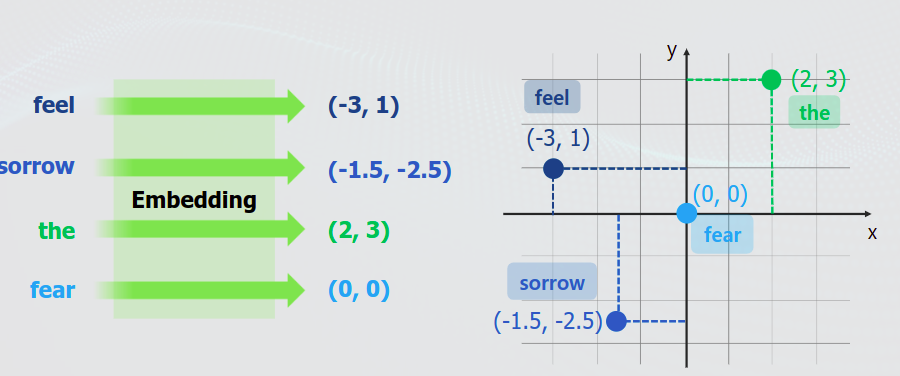
\includegraphics[width=0.6\textwidth]{images/NLP/12.png}
 \caption{ Ejemplo de embedding de 2 dimensiones \cite{NLP_28}.}
 \label{fig:Imagen_NLP_12}
\end{figure}

En conclusión, al generar embeddings nuestras palabras con significados similares estarán colocadas cercas entre sí en este espacio de embedding. En cambio, si convertimos palabras en vectores que no almacenan ningún significado, no podemos llamar a esto embeddings. 

\cleardoublepage

\paragraph{Word2vec.}\label{word2vec}

En 2013, Miklov\cite{NLP_11} sugirió un modelo para obtener una representación vectorial numérica de las palabras basado en el entrenamiento de una red neuronal, conocido como “Word2vec”. Este modelo está basado en el concepto de \textit{similitud distribucional} explicado anteriormente, permitiendo considerar el contexto del cual se toman las palabras. De esta forma, Word2vec es capaz de capturar relaciones de analogías de palabras, como por ejemplo \textit{“King - Man + Woman = Queen”}.  Estas representaciones de palabras obtenidas mediante Word2vec son nuestros \textit{word embeddings}. En la Figura \ref{fig:Imagen_NLP_13} podemos observar un ejemplo de estos word embeddings luego de entrenar un modelo Word2vec.

\begin{figure}[H]    
 \centering
 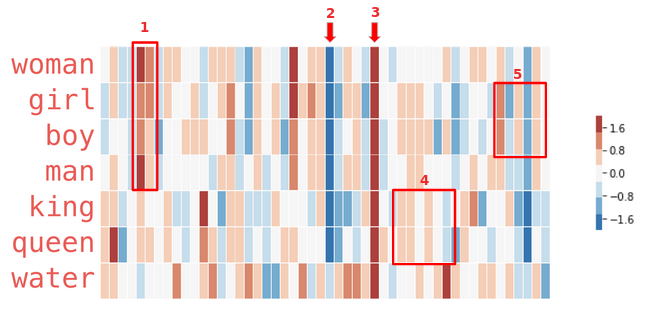
\includegraphics[width=0.8\textwidth]{images/NLP/13.png}
 \caption{Ejemplo de Word embeddings (1)\cite{datitos_nlp}.}
 \label{fig:Imagen_NLP_13}
\end{figure}

Observamos que los valores van de 1.6 a -1.6. Los valores en rojo son los más positivos y en azul los más negativos. Vemos que tenemos varias palabras que pueden tener sus similitudes y diferencias. Por ejemplo, a simple vista podemos notar de los valores marcados en recuadros rojos (1,2,3,4,5) que los embeddings permiten codificar lo siguiente:
\begin{itemize}
\item Recuadro 1: Podemos ver que estos embeddings capturan muy bien la relación entre mujer, niña, niño y hombre (ya que tienen valores muy similares en ese recuadro). Podemos suponer\footnote{Vamos a hablar en estos casos de suposiciones, ya que este embedding de salida del modelo surge en base a las dimensiones que encontró el mismo mediante el entrenamiento de grandes cantidades de texto, y que nosotros no podemos comprender a simple vista.} que la segunda columna del recuadro codifica el género y la primera la edad, entonces la combinación de esas columnas nos dan esas representaciones para esas 4 palabras. 
\item Recuadro 2: Vemos que la columna está activa en todas las palabras excepto en “water”. Esto podría significar que esta columna expresa si la palabra hace referencia a una persona (algo que el agua no tiene en común).
\item Recuadro 3: Vemos que esa columna está siempre activa, ya que el modelo encontró que todas estas palabras tienen algo en común / son símiles de alguna forma (por ej. podría expresar que son sustantivos). 
\item Recuadro 4: Vemos que en esta parte son muy parecidas las representaciones de las palabras rey y reina, quizás el modelo esté codificando allí algún significado de nobleza o de piezas de ajedrez o de tamaños de camas (esto depende con qué corpus se haya entrenado el modelo). 
\item Recuadro 5: Vemos que en esta parte son muy parecidas las representaciones de las palabras niño y niña, quizás el modelo esté codificando allí algún significado de juventud. 
\end{itemize}
En conclusión esto es lo que buscamos, \textit{obtener embeddings que permitan codificar los significados de las palabras}.

Además, debido a que los embeddings son vectores numéricos, esto nos permite operar entre ellos mediante álgebra entre vectores: ver Figura \ref{fig:Imagen_NLP_14}. Por ejemplo si restamos “king” y “man” y lo sumamos a “woman” nos da un vector muy similar al de “queen”. \textit{Esta es una gran utilidad de los embeddings, nos permiten formar relaciones entre palabras y que nuestro modelo de alguna forma -que nosotros no podemos explicar- entienda estas relaciones}.

\begin{figure}[H]    
 \centering
 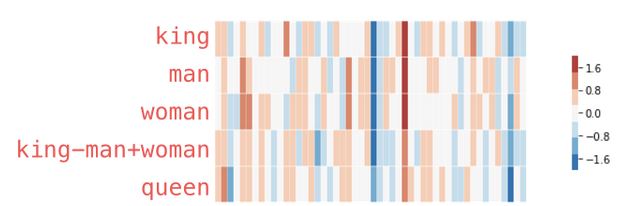
\includegraphics[width=0.8\textwidth]{images/NLP/14.png}
 \caption{Ejemplo de Word embeddings (2)\cite{datitos_nlp}.}
 \label{fig:Imagen_NLP_14}
\end{figure}

Además de Word2vec existen otros modelos para obtener dichos word embeddings, como GloVe\footnote{\url{https://nlp.stanford.edu/projects/glove/}} y Fasttext\footnote{\url{https://fasttext.cc/}}. Según estudios\cite{NLP_12, NLP_13} los resultados obtenidos mediante Word2vec, Glove y Fasttext son estadísticamente similares y ambos demuestran ser métodos competitivos. Los resultados de estos tres métodos dependen de los datos de entrenamiento que se utilicen y del dominio o tarea en la que se necesiten usar dichos embeddings. La razón por las cual en nuestra implementación utilizamos Word2vec en lugar de Glove o Fasttext es debido al futuro uso de la métrica de distancia Word Mover's Distance (WMD), ya que en el paper original de WMD\cite{wmd_paper} se utilizan embeddings obtenidos mediante Word2vec, decidiendo de esta manera utilizar la misma base en nuestra implementación.

\cleardoublepage

\paragraph{¿Cómo obtener nuestros Word embeddings?}\label{obt_word_emb}

A continuación, explicaremos cómo trabaja el modelo ‘Word2vec’ para obtener los word embeddings y de qué maneras podemos hacerlo\cite{NLP_26}.

Como mencionamos previamente, para deducir el significado de la palabra, Word2vec utiliza los conceptos de \textbf{similitudes distribucionales} e \textbf{hipótesis distribucional}. Es decir, \textit{deduce el significado usando el contexto: palabras que aparecen como “vecinas” en el texto. Entonces, el significado de una palabra viene dado por las palabras que aparecen con frecuencia cerca de ella: si dos palabras diferentes ocurren en contextos similares, es muy probable que sus significados también sean similares}.  De esta manera podemos interpretar el resultado de una \textit{palabra central} a partir de las palabras que están alrededor de ella (\textit{palabras de contexto}), o dicho de otra forma “inferir por contexto qué quiere decir esa palabra central”. 

Word2vec materializa esta idea entrenando una red neuronal y obteniendo los embeddings para cada una de las palabras del corpus de manera que el vector que representa a la palabra en el espacio vectorial / de embedding pueda capturar lo mejor posible el significado de la misma: las palabras con significados similares tienden a agruparse, y las palabras con significados muy diferentes están lejos unas de otras en dicho espacio vectorial / de embedding.

Resumidamente, Word2vec utiliza una \textit{red neuronal de 2 capas} que toma un largo corpus de texto como input, y “aprende” a representar las palabras en vectores de igual tamaño en función de los contextos en los que aparecen en el corpus. 
\\

Existen 2 manera de obtener nuestros word embeddings\cite{NLP_26}: 
\begin{enumerate}

\item \textit{Word embeddings pre-entrenados}: Entrenar nuestros propios word embeddings es un proceso costoso en cuanto a tiempo y procesamiento. Para no realizar esta tarea costosa, podemos usar word embeddings pre-entrenados. ¿Qué son estos word embeddings pre-entrenados?: alguien realizó el duro trabajo de entrenar word embeddings sobre, generalmente, un largo corpus de texto (como Wikipedia, artículos de noticias, páginas web, etc.). Estos embeddings pueden ser descargados y podemos utilizarlos para obtener los vectores de las palabras que necesitemos. Los embeddings pueden ser pensados como una larga colección de pares clave-valor, donde la clave es la palabra en el vocabulario y el valor es el correspondiente vector de la palabra. Algunos de los más populares word embeddings pre-entrenados son Word2vec de Google\footnote{\url{https://code.google.com/archive/p/word2vec/} - Sitio Web consultado el 5 de abril de 2022}, GloVe de Stanford\footnote{\url{https://nlp.stanford.edu/projects/glove/} - Sitio Web consultado el 5 de abril de 2022} y fasttext embeddings de Facebook\footnote{\url{https://fasttext.cc/docs/en/english-vectors.html} - Sitio Web consultado el 5 de abril de 2022}. Estos embeddings están disponibles en varias dimensiones (25,50,100,200,300,600, etc.).

\cleardoublepage

\item \textit{Entrenando nuestros propios word embeddings}: para entrenar y obtener nuestros propios word embeddings, Word2vec nos ofrece 2 arquitecturas disponibles, las cuales fueron propuestas en el paper original de Word2vec\cite{NLP_11}:
\begin{itemize}
\item \textit{Continuous bag of words (CBOW)}.
\item \textit{Skipgram}.
\end{itemize}

\end{enumerate}

En nuestra implementación no utilizamos word embeddings pre-entrenados ya que verificamos que no existían varias palabras en el vocabulario de dichos embeddings (también llamadas palabras \textit{out-of-vocabulary, OOV}): como por ejemplo, palabras de 2-grams como data\_scientist, $machine\_learning$, $software\_engineer$; o palabras específicas de lenguajes de programación como Python o Java. Por esta razón decidimos entrenar nuestros propios word embeddings utilizando todo el Corpus disponible de nuestros CVs de candidatos y descripciones de puestos de IT. De esta manera se tendrán en cuenta las relaciones entre palabras como $data\_science$, $machine\_learning$ y demás palabras que estén presentes en nuestros CVs o Descripciones de puestos de IT.
\\

\paragraph{CBOW vs Skipgram.}\label{cbow_vs_skip}

Como mencionamos previamente, para entrenar nuestros propios word embeddings tenemos 2 posibilidades: \textit{CBOW} o \textit{Skipgram}. A continuación realizaremos una comparación entre estas dos arquitecturas y elegiremos una de ellas para nuestra implementación.

Tanto CBOW como Skipgram aplican el concepto de semántica distribucional: las palabras obtienen su embedding teniendo en cuenta a las otras palabras que tienden a aparecer junto a ellas. Sin embargo aplican este concepto de 2 formas distintas, y armando el dataset de entrenamiento también de distinta manera. Para analizar una comparación vemos la Figura \ref{fig:Imagen_NLP_15}.

\begin{figure}[H]    %[H] es para que se ubique justo debajo del texto anterior.
 \centering
 \noindent\makebox[\textwidth]{%
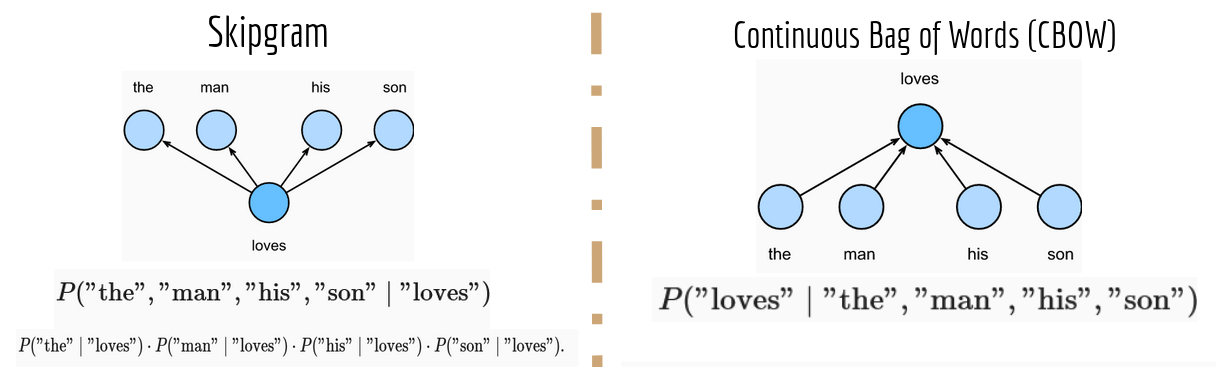
\includegraphics[width=1.2\textwidth]{images/NLP/15.png}}
 \caption{Skipgram y CBOW\cite{NLP_27}.}
 \label{fig:Imagen_NLP_15}
\end{figure}

\cleardoublepage

La diferencia principal entre CBOW y Skipgram es que en CBOW el objetivo del entrenamiento para obtener nuestros word embeddings es \textit{predecir una palabra central de un texto en función de las palabras de contexto (palabras vecinas a la palabra central)}, mientras que en Skipgram el objetivo del entrenamiento es \textit{predecir las palabras de contexto en base a la palabra central}. Estas diferencias podemos observarlas en la Figura \ref{fig:Imagen_NLP_15}.

A continuación realizaremos una comparación entre las fórmulas matemáticas de Skipgram y CBOW. 
\begin{itemize}

\item En \textbf{Skipgram} se calcula cuál es la probabilidad de las palabras de contexto (las que tratamos de adivinar / predecir) dada la palabra central. En el ejemplo de la  Figura \ref{fig:Imagen_NLP_15} calcula la probabilidad de las palabras “the”, “man”, “his” y “son”, dado que la palabra central es “loves”. Como vemos, esto se traduce en la multiplicación de cada una de las probabilidades condicionales individuales: \textit{probabilidad de la palabra de contexto “the” dada la palabra central “loves” $x$ la probabilidad de “man” dado “loves” $x$ la probabilidad de “his” dado “loves” $x$ la probabilidad de “son” dado “loves”}. Esto termina siendo \textit{dos productorias}: ver Fórmula \ref{eq:ecuacion_4_NLP}. 

\begin{equation}\label{eq:ecuacion_4_NLP}
\prod_{t=1}^{T} \; \prod_{-m \leq j \leq m, j \neq 0}  P(w^{(t+j)} | w^{(t)}) \qquad \text{(Ver \cite{NLP_27})}
\end{equation}
\begin{center}
\textit{Cálculo de probabilidades mediante Skipgram.}
\end{center}

Teniendo en cuenta que:
\begin{itemize}
\item \textit{La primer productoria} ($ \prod_{-m \leq j \leq m, j \neq 0} $) es aplicada sobre la “ventana de contexto” \footnote{Ventana de contexto (o Context Window, “C”) es una ventana de tamaño $m$ que podemos colocar en cualquier parte de nuestro corpus de texto, y define qué tan largo o corto tomamos el contexto (palabras de contexto) para realizar el entrenamiento de nuestro modelo y obtener nuestra representación vectorial\cite{NLP_26}. La cantidad de palabras a usar como tamaño de ventana es un \textit{hiper-parámetro} de nuestro modelo que se define a partir de nuestros datos, y que discutiremos más adelante en la sección \textit{\nameref{hiper_par_word2vec}} }: es decir, $j$ va desde un $-m$ hasta un $+m$, donde ese m es el tamaño de nuestra ventana (en este ejemplo es 2, por lo que tomamos 2 palabras a la izquierda y otras 2 a la derecha de la palabra central, obteniendo como palabras de contexto “the”, “man”, “his”, “son”). Y lo que se calcula en $P(w^{(t+j)} | w^{(t)})$ es la probabilidad de la palabra de contexto $w^{(t+j)}$ dada la palabra central $w^{(t)}$. De esta manera multiplicamos todas esas probabilidades y obtenemos la probabilidad de 1 palabra. 
\item Luego, en la \textit{segunda productoria} ($\prod_{t=1}^{T}$) multiplicamos por todas las otras palabras de nuestro corpus, ya que $T$ = palabras de nuestro corpus.  

\end{itemize}

\item En cambio, en \textbf{CBOW} es al revés: se calcula cuál es la probabilidad de la palabra central (la que tratamos de adivinar / predecir) dado que tenemos todas las palabras de contexto. En el ejemplo de la  Figura \ref{fig:Imagen_NLP_15}  calcula la probabilidad que la central sea “loves” dadas las palabras de contexto “the”, “man”, “his”, “son”. En este caso esto se traduce a \textit{una sola productoria} (la que itera sobre las palabras de nuestro corpus de texto T): Fórmula \ref{eq:ecuacion_8_NLP}.

\begin{equation}\label{eq:ecuacion_8_NLP}
\prod_{t=1}^{T} P(w^{(t)} | w^{(t-m)}, …, w^{(t-1)}, w^{(t+1)}, …, w^{(t+m)} )  \qquad \text{(Ver \cite{NLP_27})}
\end{equation}
\begin{center}
\textit{Cálculo de probabilidades mediante CBOW.}
\end{center}


\end{itemize}

Entonces, ¿qué nos conviene elegir: CBOW o Skipgram?. Para responder a esto detallaremos las conclusiones obtenidas del paper original de Word2vec\cite{NLP_11}:
\begin{itemize}
\item \textit{Skipgram} necesita menor cantidad de datos y se encontró que representa mejor las palabras raras: debido a que Skipgram por cada palabra genera más ejemplos, las palabras que aparecen pocas veces (“raras” o infrecuentes) están mejor representadas en el dataset. 
\item \textit{CBOW} funciona más rápido (ya que por lo que vimos anteriormente hace menos cuentas, solo una productoria) y tiene una mejor representación para palabras más frecuentes.
\end{itemize}

Es por esto que para nuestra implementación \textbf{se optó por utilizar Skipgram}; debido a que nuestro dataset de entrenamiento no es muy grande (nuestro vocabulario consiste en 60713 palabras) y necesitamos utilizar esta arquitectura que funciona mejor para pocos datos. Además, como mencionamos previamente, otro punto a favor de Skipgram es que {nos permite representar mejor palabras “raras” o infrecuentes}, y esto es una ventaja en IT ya que cada vez más cantidad de lenguajes y tecnologías van apareciendo, por lo que aunque una palabra aparezca pocas veces en nuestros corpus de texto, hay que tenerlas en cuenta y tratar de representarlas lo mejor posible.

El funcionamiento del modelo Skipgram para obtener nuestros word embeddings está detallado en la sección \textit{\nameref{obt_skip}}. Previamente a esto, explicaremos el concepto de vectores de tipo \textit{one hot encoding}, concepto necesario para entender el modelo Skipgram.
\\

\paragraph{One hot encoding.}\label{one_hot_enc}

\textit{One hot encoding} es una forma de representación vectorial que consiste en representar a cada palabra como un vector único con un único elemento (o columna) siendo 1 y el resto de los elementos (o columnas) = 0. El producto interno de dos vectores de palabras diferentes siempre es 0, es decir, cada palabra siempre es \textit{ortogonal} a todas las demás palabras\cite{NLP_9}.

Al igual que BoW y TF-IDF,  one hot encoding también es una representación dispersa, de alta dimensionalidad y discreta: presentando todas las desventajas ya previamente detalladas en la sección \textit{\nameref{desv_bow_tfidf}}. Algo que se diferencia de BoW y TF-IDF es que estas son representaciones vectoriales para cada oración / documento de texto; en cambio one hot encoding, al igual que word embeddings, son representaciones vectoriales para cada \textit{palabra} de la oración / documento de texto. 

En la Figura \ref{fig:Imagen_NLP_16} podemos observar la representación de 4 palabras como vectores one hot encoding. Mientras que en la Figura \ref{fig:Imagen_NLP_17}, considerando un tamaño de vocabulario de 1000, observamos la desventaja de ser una representación \textit{dispersa} y de \textit{alta dimensionalidad}: este vector tendrá 999 ceros y 1 solo uno.

\begin{figure}[H] %[H] es para que se ubique justo debajo del texto anterior.
\begin{minipage}[b]{0.5\linewidth}
\centering
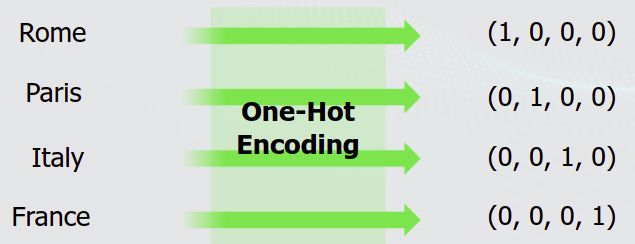
\includegraphics[width=\linewidth]{images/NLP/16.png}
\caption{One Hot Encoding (1)\cite{NLP_28}.}
\label{fig:Imagen_NLP_16}
\end{minipage}
\hspace{0.5cm}
\begin{minipage}[b]{0.5\linewidth}
\centering
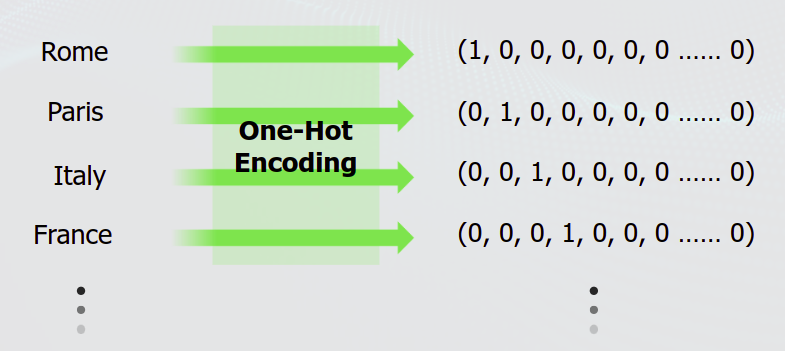
\includegraphics[width=\linewidth]{images/NLP/17.png}
\caption{One Hot Encoding (2)\cite{NLP_28}.}
\label{fig:Imagen_NLP_17}
\end{minipage}
\end{figure}

En la Figura \ref{fig:Imagen_NLP_18} se visualiza la otra desventaja de estos vectores: ser una representación \textit{discreta}. De esta manera el vector que representa a la palabra no representa su significado ni permite capturar las relaciones entre las palabras, únicamente expresa su ubicación en un espacio N-dimensional (donde N es el tamaño del vocabulario). Como tenemos un vector para cada palabra, donde todos los vectores son todos distintos entre sí, cualquier par de vectores one hot es \textit{ortogonal} (porque tienen un 1 en una dimensión distinta entre sí), por lo tanto no hay una noción natural de similitudes entre ellos: las palabras ‘uva’ y ‘arándano’ son tan diferentes y tan parecidas como las palabras ‘uva’ y ‘elefante’ (todas las palabras son igual de diferentes). 

\begin{figure}[H]    
 \centering
 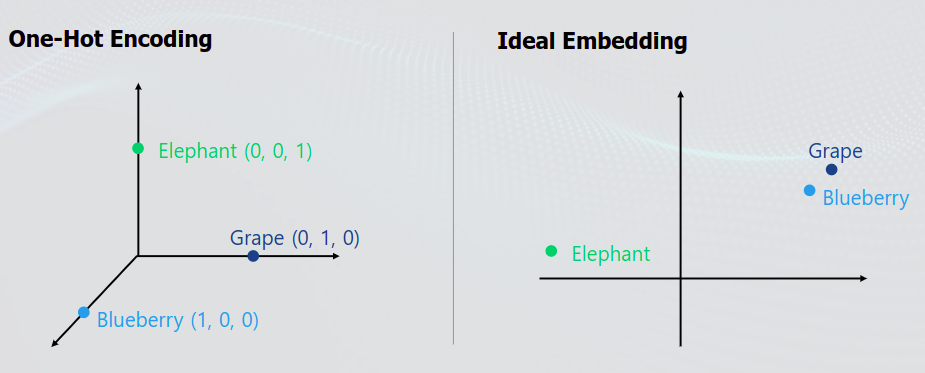
\includegraphics[width=0.8\textwidth]{images/NLP/18.png}
 \caption{One Hot Encoding (3)\cite{NLP_28}.}
 \label{fig:Imagen_NLP_18}
\end{figure}

Sin embargo, debido a que one hot encoding permite representar a nuestras palabras del vocabulario mediante vectores, aunque muy vagamente -ya que no permiten capturar las relaciones entre palabras-, estos vectores son utilizados para alimentar a nuestro modelo Word2vec (en la capa de entrada de la red neuronal) para obtener al final -luego del entrenamiento- nuestras representaciones densas (Word embeddings).

\cleardoublepage

\paragraph{Obteniendo nuestros Word embeddings con Skipgram.}\label{obt_skip}

Ya habiendo explicado previamente los conceptos básicos de redes neuronales y vectores de tipo one hot encoding, ahora explicaremos el modelo Skipgram, el cual utilizamos para entrenar y obtener nuestros Word embeddings. Para esto, tomaremos como ejemplo la oración “The quick brown fox jumps over the lazy dog” como nuestro corpus de texto de ejemplo.

Como mencionamos previamente, el objetivo de Word2vec utilizando Skipgram es predecir cuál es la probabilidad que aparezcan todas las palabras de contexto a partir de la palabra central / dado que se conoce esta palabra central. Dicho de otra manera, la tarea principal en Skipgram consiste en construir un \textit{modelo de lenguaje} que correctamente prediga las palabras de contexto dada la palabra central. 

Un modelo de lenguaje es un modelo estadístico que trata de otorgar una distribución de probabilidad sobre secuencias de palabras; permitiendo así, por ejemplo, predecir cuál es la siguiente palabra. Dada una oración de $m$ palabras, asigna una probabilidad $Pr(w_1, w_2, …, w_m)$ a la oración completa. El objetivo del modelo de lenguaje es asignar probabilidades de forma que otorgue una alta probabilidad a oraciones “buenas” y bajas probabilidades a oraciones “malas”. Con “buenas” nos referimos a oraciones que son semántica y/o sintácticamente correctas; y por “malas” nos referimos a oraciones que son incorrectas semántica y/o sintácticamente\footnote{En el análisis sintáctico se analiza la sintaxis, que incluye la acción de dividir una oración en cada uno de sus componentes. En cambio, en el análisis semántico se busca entender el significado de la oración. Las palabras pueden tener múltiples significados, el objetivo en este caso es identificar el significado apropiado por medio del contexto de la oración.}. De esta manera, para la oración “The cat jumped over the dog” tratará de asignar una probabilidad cercana a 1.0, mientras que para la oración “jumped over the the cat dog” asignará una probabilidad cercana a 0.0\cite{NLP_26}. Este cálculo de probabilidades para Skipgram es el descrito anteriormente en la Fórmula \ref{eq:ecuacion_4_NLP}.

Algo a destacar de los modelos de lenguajes es que tienen una gran \textit{ventaja} sobre la mayoría de los otros modelos de aprendizaje automático. Esa ventaja es que tenemos un montón de datos de texto para entrenarlos: los podemos obtener de libros, artículos, contenido de millones de páginas web, etc. En otros modelos de aprendizaje automático, como en modelos de detección de imágenes, no tenemos “naturalmente” los datos, ya que generalmente necesitamos datos recopilados especialmente y que cuenten con un preprocesamiento de etiquetado manual. 

Siguiendo con nuestro ejemplo, para nuestro corpus “The quick brown fox jumps over the lazy dog” utilizaremos un tamaño de ventana de contexto = 2.  Nuestro primer objetivo es armar un \textit{dataset} a partir del corpus para alimentar y entrenar al modelo, ya que como mencionamos anteriormente, el significado de las palabras vienen a partir de las \textit{similitudes distribucionales}. Para esto realizamos una serie de iteraciones: en la Figura \ref{fig:Imagen_NLP_19} podemos observar una iteración específica dentro del modelo Skipgram, donde a partir de la palabra central “jumps” (en azul), se intenta predecir/adivinar cada una de las palabras de contexto (en este caso “brown”, “fox”, “over” y “the”).  Esto únicamente constituye un paso, Skipgram repite esto para cada palabra de nuestro corpus siendo la palabra central. Para esto \textit{se desplaza la ventana de contexto}: vemos en la Figura \ref{fig:Imagen_NLP_20}  que para la siguiente iteración nos movemos una palabra a la derecha, cambiando de esta manera nuestras palabras de contexto y nuestra palabra central (la cual pasa a ser “over”). Esta ventana se desplazará hasta recorrer todo el corpus de texto.

\begin{figure}[H]    
 \centering
 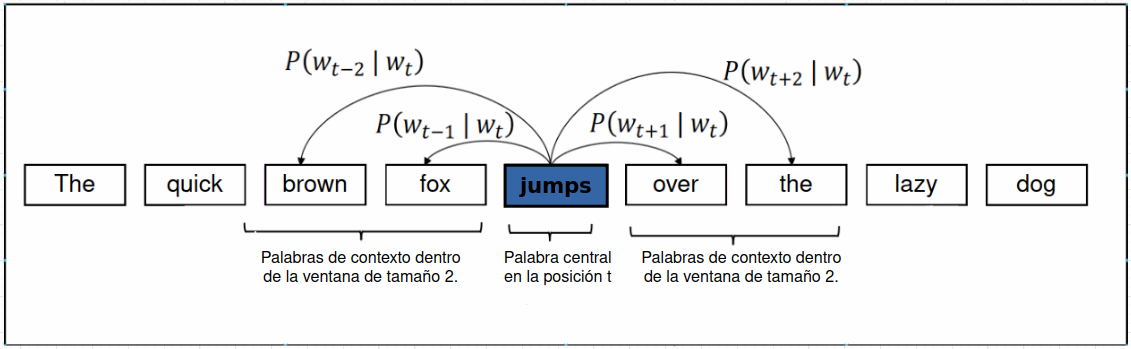
\includegraphics[width=1\textwidth]{images/NLP/19.png}
 \captionsetup{justification=centering,margin=3cm}
 \caption{Skipgram: dada la palabra central se predicen las palabras de contexto.}
 \label{fig:Imagen_NLP_19}
\end{figure}

\begin{figure}[H]    
 \centering
 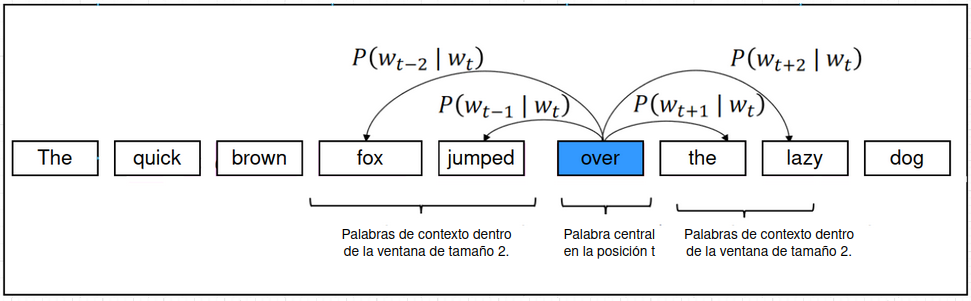
\includegraphics[width=1\textwidth]{images/NLP/20.png}
 \caption{Skipgram: próxima iteración.}
 \label{fig:Imagen_NLP_20}
\end{figure}

De esta manera se obtiene el \textit{dataset} que será utilizado para entrenar Skipgram y obtener al final del entrenamiento nuestros embeddings. Explicado de una forma más general, podemos decir que para obtener nuestro dataset corremos una \textit{ventana deslizante de contexto de tamaño $C$} sobre nuestro corpus de texto para obtener un set de $2C+1$ palabras que tendremos en consideración en cada paso. La palabra central en nuestra ventana es $X$, y las $C$ palabras a cada lado de la palabra central son $Y$. Esto nos da $2C$ puntos de datos. Un único punto de datos consiste en un par \textit{(índice de la palabra central, índice de la palabra target o de contexto)}. Luego deslizamos la ventana 1 palabra a la derecha del corpus y repetimos el proceso. De esta manera, deslizamos la ventana sobre todo nuestro corpus de texto para crear nuestro \textit{dataset de entrenamiento}: Figura \ref{fig:Imagen_NLP_21}. 

\begin{figure}[H]    
 \centering
 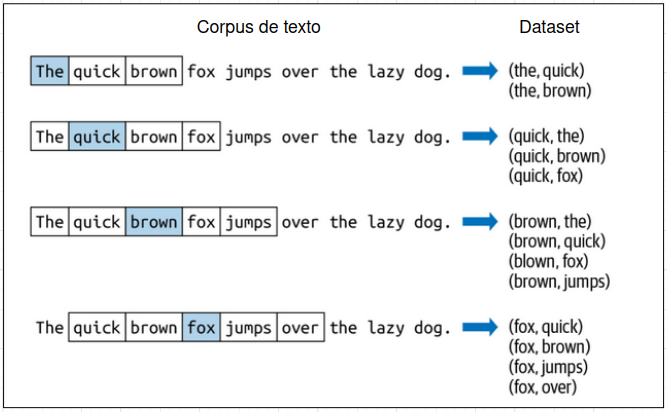
\includegraphics[width=0.8\textwidth]{images/NLP/21.png}
 \captionsetup{justification=centering,margin=4cm}
 \caption{Preparando nuestro dataset para Skipgram (con $C$ = 2)\cite{NLP_26}.}
 \label{fig:Imagen_NLP_21}
\end{figure}

Como vemos en la imagen anterior, exceptuando los inicios y finales de nuestros corpus (donde las ventanas deslizantes no llegan a estar completas), podemos observar que dada una palabra central, la misma en el dataset va a aparecer $2xC$ veces: por ejemplo, para la tercer iteración, brown aparecerá en el dataset $2x2=4$ veces. Es por esto que con Skipgram se representan mejor las palabras infrecuentes / raras a comparación de CBOW: las palabras que aparecen pocas veces, en el dataset aparecen muchas veces.

En este dataset (Figura \ref{fig:Imagen_NLP_21}) la primer palabra de nuestro par (la palabra central) será tratada como la palabra de entrada a la red, y la segunda palabra de nuestro par (palabra de contexto) será tratada como la salida o posible resultado. Vemos que esto al final es una tarea de \textit{clasificación}: dado que se sabe cual es esta palabra (input word) se debe predecir cuál palabra de contexto le sigue.

Por último, algo que puede generar curiosidad es: ¿qué sucede en el entrenamiento con las palabras que aparecen más de una vez en nuestro Corpus? Y ¿qué sucede con las palabras polisémicas\footnote{Palabras que tienen más de un significado.}? Estas preguntas son respondidas en el Anexo: ver sección \textit{\nameref{anexo_polisem}}.

\cleardoublepage

\paragraph{Arquitectura del modelo Skipgram.}\label{skipgram}

En la Figura \ref{fig:Imagen_NLP_22} podemos observar: a la izquierda, la red neuronal de 2 capas utilizada para entrenar a nuestro modelo Skipgram, mientras que a la derecha, un “resumen” compactado de la misma utilizando el ejemplo de la iteración de la Figura \ref{fig:Imagen_NLP_19}.  Observamos que nuestra arquitectura Skipgram tiene:
\begin{itemize}
\item Un vector de capa de entrada de $V$ dimensiones -siendo $V$ el tamaño de nuestro vocabulario-.
\item Un vector de capa oculta de $N$ dimensiones -siendo $N$ el tamaño (dimensión) del embedding (de la matriz $W$)-. 
\item Un vector de salida también de $V$ dimensiones. 
\end{itemize}

Además, cabe destacar que la capa oculta \textit{no posee una función de activación}, mientras que en la capa de salida se utiliza la \textit{función softmax}. 

\begin{figure}[H]    
 \centering
 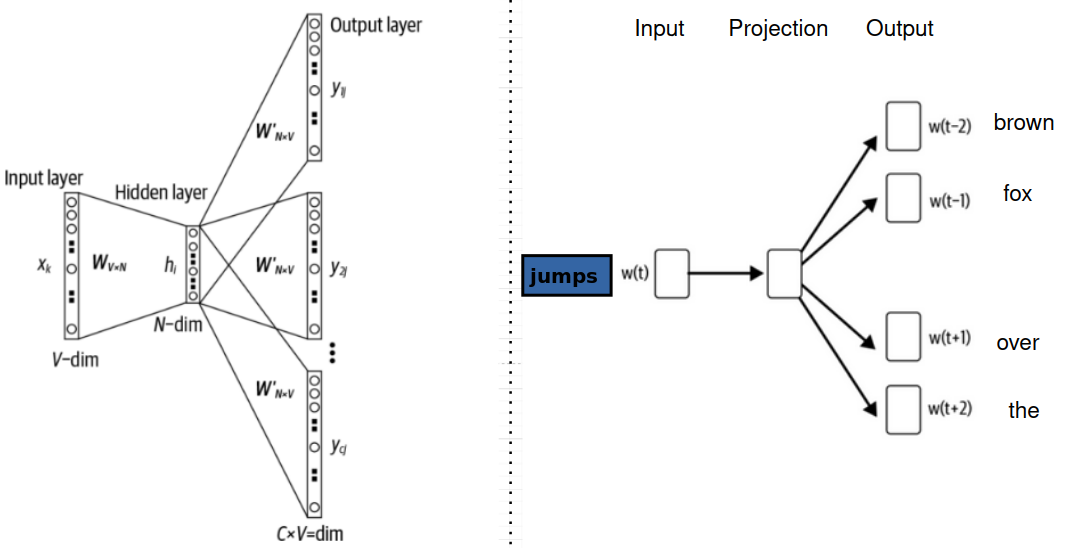
\includegraphics[width=1\textwidth]{images/NLP/22.png}
 \caption{Arquitectura básica Skipgram\cite{NLP_26}.}
 \label{fig:Imagen_NLP_22}
\end{figure}

En la Figura \ref{fig:Imagen_NLP_23} podemos observar en mayor detalle la arquitectura de Skipgram. En este ejemplo se considera un tamaño de vocabulario = 8 ($V$), un tamaño de embedding = 3 ($N$) y un tamaño de ventana = 1 ($C$). Como $C=1$, tomaremos como palabras de contexto 1 palabra de cada lado de la palabra central.

\begin{figure}[H]  
\centering
\noindent\makebox[\textwidth]{%
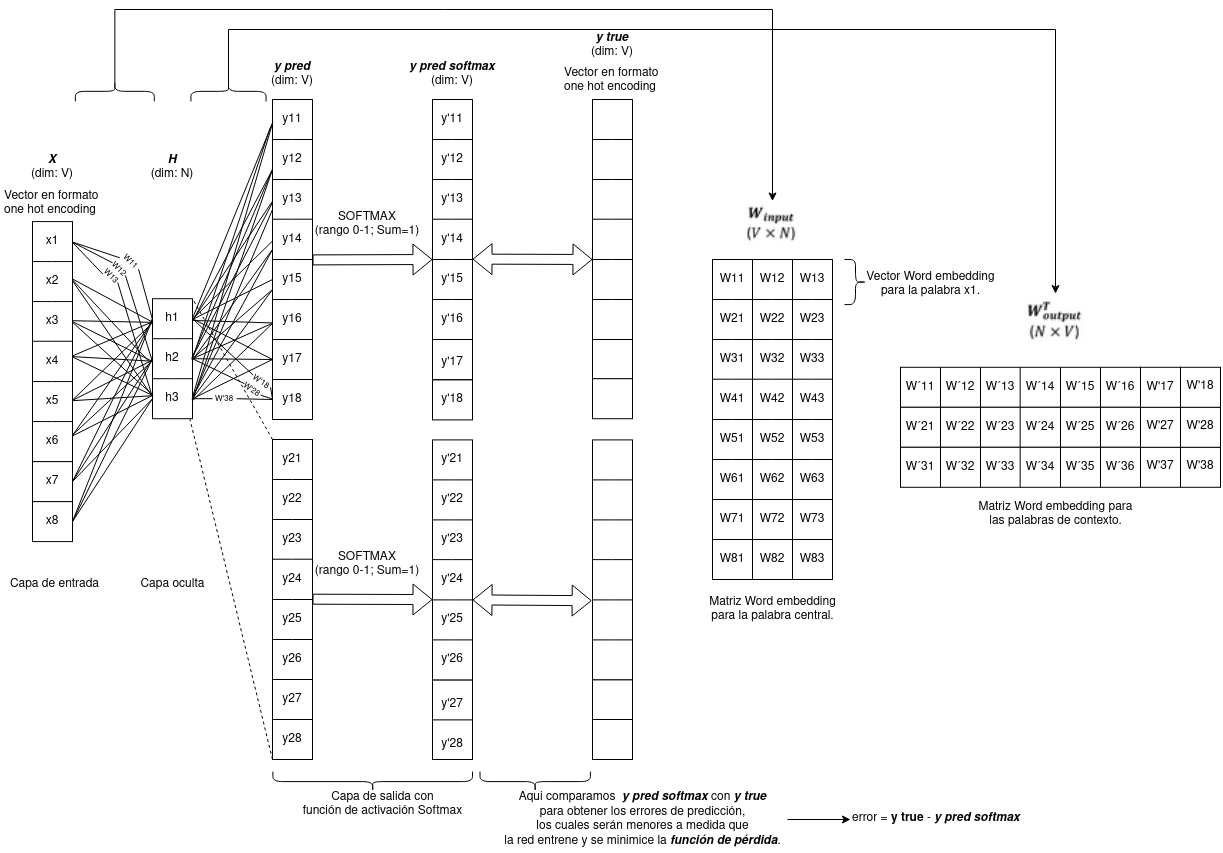
\includegraphics[width=1.2\textwidth]{images/NLP/23.png}}
\caption{Arquitectura Skipgram con $V=8$, $N=3$, $C=1$.}
\label{fig:Imagen_NLP_23}
\end{figure}

Debido a que $C=1$, observamos 2 vectores de salida \textit{y pred}. Sin embargo esto es simplemente para una mejor visualización, ya que la salida realmente para cada iteración es un único vector formada por 8 posiciones (o neuronas) debido a que nuestro modelo entrena con un \textit{par} de palabras: primero $(central1, contexto1)$ y luego $(central1, contexto2)$ -considerando $C=1$-. 

El proceso de entrenamiento de esta red neuronal se explicará en detalle en la sección \textit{\nameref{ent_costo_softmax}}. Lo que hay que tener en consideración, es que al final del mismo, \textit{nuestro objetivo \textbf{no} es obtener la salida de la red; nuestro objetivo es extraer $W$, la cual será nuestra matriz de embedding que utilizaremos para representar los textos}. Por esta razón se considera que mediante Word2vec estamos realizando una “\textit{tarea falsa}”, ya que realmente no estamos interesados en la predicción del modelo para la tarea en que fue entrenada, sino en el subproducto del modelo: nuestros word embeddings.

\cleardoublepage

\paragraph{Entrenamiento y función de costo con Softmax.}\label{ent_costo_softmax}

Como mencionamos previamente, la capa oculta \textit{no posee una función de activación} y en la capa de salida se usa la \textit{función softmax}. Además, las palabras que ingresan a la capa de entrada a lo largo de cada iteración de entrenamiento deben estar representadas en formato one hot encoding (ver sección \textit{\nameref{one_hot_enc}}).

Resumidamente, el entrenamiento de nuestro modelo Word2vec mediante la arquitectura Skipgram consiste en el ingreso de un par de palabras $(central, contexto)$, donde la palabra central será puesta en la capa de entrada y la de contexto funcionará como target en la capa de salida. Luego mediante \textit{forward propagation} se obtiene el valor de cada neurona de la capa de salida utilizando la función softmax. Este procedimiento anterior se repite hasta que todas las palabras de nuestro corpus hayan actuado como palabra central e ingresado a la red como un par $(central, contexto)$.
Al tener todas las salidas de cada una de las combinaciones palabra central y contexto, lo que se hace es comparar estas salidas predichas con las salidas reales correspondientes de la palabra de contexto / target, y utilizar \textit{back propagation} para actualizar los parámetros de nuestro modelo (las matrices $W$ y $W’$) minimizando nuestra función de costo $J$. Este procedimiento que incluye forward propagation y back propagation se realiza en un número de $epochs$ determinado. 

A continuación, describiremos en detalle este ciclo iterativo de procesos del entrenamiento. Como se trata de un modelo de red neuronal, este proceso general fue explicado anteriormente en la sección \textit{\nameref{entren_ann}}, solo que ahora adaptaremos la explicación para Skipgram. Al final de este ciclo de entrenamiento el objetivo es \textit{extraer la matriz $W$ (nuestra matriz de Word embeddings)}.

El ciclo de entrenamiento utilizando Skipgram consiste en las siguientes fases:
\begin{enumerate}

\item \textbf{Inicialización aleatoria} por única vez de las matrices de pesos ($W input$ -o $W$- y $W output$ -o $W'$- en nuestro caso), los cuales son los parámetros ($\theta$) de nuestro modelo de red neuronal.  

\item \textbf{Forward propagation}. En este proceso se realizan los cálculos necesarios para obtener nuestras salidas -\textit{y pred softmax}-. Vamos a dividirlo en dos sub-pasos:

\begin{itemize}

\item 2.1. \textit{Forward propagation (capa de entrada a capa oculta)}: En este paso se calcula el valor de cada neurona de la capa oculta. Para esto se utiliza la palabra central de entrada (la cual está codificada en formato one hot encoding) en conjunto con su fila correspondiente de la matriz de embedding $W$ -de tamaño $V x N$- (la cual representa los pesos de entrada de nuestra red). Como el vector de entrada únicamente es 1 para la palabra en cuestión (o dicho de otra forma, por cada iteración hay únicamente una neurona activa en la capa de entrada), entonces los valores de las neuronas de la capa oculta son directamente los valores de los pesos que corresponden a esa única neurona de la capa de entrada activa: por ejemplo, considerando que tenemos 3 neuronas en la capa oculta ($N=3$) y que nuestro vector de entrada es de 8 ($V=8$), nuestra primer entrada sería $[1,0,0,0,0,0,0,0]$, por lo que el valor de la primer neurona de la capa oculta ($h1$) será de $1$ $x$ $w11$, $h2 = w12$ y $h3 = w13$.\\ \\

\item 2.2. \textit{Forward propagation (capa oculta a capa de salida)}: En este paso se calcula el valor de cada neurona de la capa de salida luego de pasar por la función de salida softmax (vector \textit{y pred softmax}).  Debido a que la capa oculta no tiene función de activación, entonces los valores calculados en el paso 2.1 pasan directamente a la capa de salida. De esta manera, los valores de las neuronas de la capa de salida se calculan multiplicando el vector $H$ que nos dió anteriormente con otra matriz $W’$ -de tamaño $N x V$-. Esto nos dará un vector \textit{y pred} de tamaño $V$, el cual alimentará a una función softmax para obtener una distribución de probabilidades sobre el espacio de nuestro vocabulario (-\textit{y pred softmax}-). 
\\

Para cada una de las combinaciones entre palabras centrales y de contexto se realizan los pasos 2.1 y 2.2 hasta que todas las palabras de nuestro corpus hayan actuado como palabra central, obteniendo al final todas las salidas -\textit{y pred softmax}- de cada una de las combinaciones palabra central y contexto. 

\end{itemize}

\item \textbf{Cálculo de función de costo}:  Luego de obtener las distribuciones -\textit{y pred softmax}- (valor predicho) para cada combinación de palabras $(central, contexto)$, estas son comparadas con los vectores de salida -\textit{y true}- correspondientes (que tienen las etiquetas reales y al igual que los vectores de entrada están codificados en formato one hot encoding), computándose de esta manera el \textit{error (o loss)} de clasificación (entre el valor predicho y el real) mediante el cálculo de la \textit{función de costo (loss function) $J(\theta)$}: Fórmula \ref{eq:ecuacion_11_NLP} que veremos más adelante. Esta función de costo tiene en cuenta todas las palabras de nuestro texto $T$, y toma todos los pares correspondientes de palabras $(central, contexto)$ dependiendo de nuestra ventana de contexto de tamaño $m$.

\item \textbf{Backpropagation}: Se aplica este proceso utilizando el algoritmo de optimización \textit{descenso del gradiente} para poder ajustar / modificar las matrices $W input$ y $W output$  (que juntos forman $\theta$) \textit{con el objetivo de minimizar la función de costo $J(\theta)$ obtenida en el paso 3}, y con ello minimizar el error de clasificación. No se detallará este procedimiento aquí porque no entra dentro de los objetivos de este trabajo. Sin embargo, lo que hay que tener en cuenta es que se utiliza la ecuación general \ref{eq:ecuacion_9_ANN} explicada anteriormente para actualizar los parámetros de nuestra red neuronal. 

\item Volver al paso 2 hasta completar la cantidad de epochs seteados como \textit{hiper-parámetro} de nuestro modelo. 

\end{enumerate}

Cabe destacar que este entrenamiento descrito tiene en cuenta el uso del \textit{algoritmo de gradiente descendiente “básico”}. Con este método se calcula el error o función de costo luego de haber pasado todos los datos de entrenamiento a través de la red de una sola vez. De esta manera, luego de calcular forward propagation \textit{para todos los datos de entrada}, se computa la función de costo y se aplica backpropagation realizando la actualización de los pesos. Todo este “bloque” de procedimiento se aplica por epoch. Por lo tanto, con este método de gradiente descendiente se calcula una función de costo y se realiza una sola actualización de los pesos por cada epoch.

Otra opción hubiera sido utilizar el algoritmo de \textit{gradiente descendiente estocástico} (stochastic gradient descent, \textit{SDG}). Con este método se calcula el error o función de costo luego de haber pasado solo un ejemplo de nuestros datos de entrenamiento a través de la red. De esta manera, por cada ejemplo de entrenamiento se calcula forward propagation, luego se computa la función de costo y se aplica backpropagation realizando la actualización de pesos. Todo esto nuevamente se aplica por cada epoch. Si tuviéramos 100 ejemplos entonces calculariamos 100 veces la función de costo y los pesos se actualizarian 100 veces. En la práctica este método resulta más rápido que el gradiente descendiente “básico”.  Sin embargo, SDG no se utilizó en este Proyecto debido a que por defecto no se encuentra la opción de setear el algoritmo de gradiente descendiente en la implementación de Word2vec de gensim, la cual se basa en el paper original de Word2vec\cite{NLP_11} donde describe la función de costo mediante el uso de GD básico, teniendo en cuenta el entrenamiento de todas las palabras de nuestro texto T dentro de todas las ventanas de contexto. En caso de utilizar SDG, la función de costo debería expresarse individualmente por cada palabra de nuestro texto $T$ teniendo en cuenta las combinaciones dentro de la ventana de contexto de tamaño $m$: Fórmula \ref{eq:ecuacion_12_NLP} que veremos más adelante.

Para comprender mejor las iteraciones de entrenamiento, se recomienda consultar el Anexo (sección \textit{\nameref{anexo_word_emb}}) donde se detalla un ejemplo concreto del entrenamiento del modelo Skip gram con función de salida softmax utilizando el algoritmo de gradiente descendiente “básico”. En este ejemplo se toma a la oración “The quick brown fox jumps over the lazy dog” como nuestro corpus de texto con el cual entrenará el algoritmo.

Como podemos observar, todo este entrenamiento tiene como objetivo minimizar la \textit{función de costo} para realizar una correcta predicción. La \textit{función de costo $J(\theta)$} de Skipgram se basa en la \textit{función de verosimilitud $L(\theta)$}, la cual es prácticamente la que vimos en la Fórmula \ref{eq:ecuacion_4_NLP}. La reescribimos como la Fórmula \ref{eq:ecuacion_10_NLP}: aquí se calcula, para cada posición del texto $t = 1, ..., T$ (donde $T$ es nuestro corpus de texto) y para cada ventana de contexto de tamaño fijo $m$, cuál es la probabilidad de que una palabra $(w^{(t+j)})$ sea contexto de una palabra central ($w^{(t)}$), dada esa palabra ($w^{(t)}$) y los parámetros del modelo $(\theta)$ -que en nuestro caso son las matrices de pesos $W$ y $W’$-. De esta manera, con $L(\theta)$ obtenemos la probabilidad de generar todas las palabras de contexto dada cualquier palabra central.

\begin{equation}\label{eq:ecuacion_10_NLP}
L(\theta) = \prod_{t=1}^{T} \; \prod_{-m \leq j \leq m, j \neq 0}  P(w^{(t+j)} | w^{(t)} ; \theta) \qquad \text{(Ver \cite{NLP_27})}
\end{equation} 
\begin{center}
\textit{Función de verosimilitud Skipgram.}
\end{center}

A  $L(\theta)$  se le aplica el logaritmo y se le coloca un menos por delante para que de esta manera sea minimizable, obteniendo así la función de costo a minimizar $J(\theta)$ (Fórmula \ref{eq:ecuacion_11_NLP}), la cual es la \textit{verosimilitud logarítmica negativa media}. La mejor minimización de esta función la obtendremos cuando la probabilidad de que aparezca la palabra $w^{(t+j)}$ dada $w^{(t)}$ sea 1 (ya que el logaritmo de 1 es 0, siendo este el valor mínimo). Cuando el valor de la probabilidad es menor que 1 los valores se hacen muy negativos, pero al colocarle el menos se hacen muy positivos. Además, algo a tener en cuenta es que transformamos las \textit{productorias} de la  Fórmula \ref{eq:ecuacion_10_NLP} en \textit{sumatorias} en la Fórmula \ref{eq:ecuacion_11_NLP}; ya que le estamos aplicando el logaritmo a la función $L(\theta)$, y el logaritmo del producto es la suma de los logaritmos.
\cleardoublepage

\begin{equation}\label{eq:ecuacion_11_NLP}
J(\theta) = -\frac{1}{T} log L (\theta) = -\frac{1}{T} \sum_{t=1}^{T} \sum_{-m \leq j \leq m, j \neq 0} log P(w^{(t+j)} | w^{(t)} ; \theta)    \qquad \text{(Ver \cite{NLP_27})}
\end{equation}
\begin{center}
\textit{Función de costo Skipgram.}
\end{center}

Como mencionamos anteriormente, esta fórmula es teniendo en cuenta nuestra implementación con el algoritmo de gradiente descendiente “básico”. Si quisiéramos implementar el algoritmo SGD, nuestra función de costo quedaría representada como la Fórmula \ref{eq:ecuacion_12_NLP}, la cual se calcularía luego de realizar cada una de las iteraciones individuales de las palabras $w(t)$ teniendo en cuenta  cada posición de la ventana de contexto. 

\begin{equation}\label{eq:ecuacion_12_NLP}
J (\theta;w^{(t)}) = - \sum_{-m \leq j \leq m, j =! 0} log P(w^{(t+j)} | w^{(t)} ; \theta)   \qquad \text{(Ver \cite{NLP_27})}
\end{equation}
\begin{center}
\textit{Función de costo Skipgram utilizando SGD.}
\end{center}

Ahora, ¿cómo calculamos la probabilidad $P(w^{(t+j)} | w^{(t)} ; \theta)$?. Vamos a omitir los parámetros de nuestro modelo $(\theta)$ para simplificar la notación. Utilizaremos dos vectores densos por cada palabra $w$:
\begin{itemize}
\item $v_w$: vector de tamaño $d$ para simbolizar cuando $w$ es la palabra central $w_c$, donde $d$ es el tamaño de palabras de nuestro vocabulario.
\item $u_w$: vector de tamaño $d$ para simbolizar cuando $w$ es una palabra de contexto $w_o$.
\end{itemize}

De esta manera, en la Fórmula \ref{eq:ecuacion_15_NLP} se describe cómo obtener la probabilidad de que $w_o$ sea una palabra de contexto (con índice $'o'$ en nuestra secuencia de textos T) dada una palabra central $w_c$ (con índice $'c'$ en el diccionario del corpus).  El cálculo de la misma es similar a la que se usa cuando queremos calcular la probabilidad de salida de distintas clases en clasificación utilizando la función softmax (ver Fórmula \ref{eq:ecuacion_7_ANN}) donde se calcula la probabilidad de todas las clases sumadas y por cada probabilidad se divide la misma, obteniendo así una \textit{distribución} (ya que la suma de todas las probabilidades resultantes como salida dan 1). 

\begin{equation}\label{eq:ecuacion_15_NLP}
P(w_o, w_c) = \frac{exp(u_{o}^{T} v_c)}{\sum_{W \in V} exp(u_{W}^{T} v_c)}    \qquad \text{(Ver \cite{NLP_27})}
\end{equation}
\begin{center}
\textit{ Probabilidad de que $w_o$ sea una palabra de contexto dada \\ una palabra central $w_c$ (función de salida softmax).}
\end{center}

Teniendo en cuenta que:
\begin{itemize}
\item $u_o$ = vector de la palabra de contexto ($o$ = outside/contexto).
\item $v_c$ = vector de la palabra central ($c$ = central).
\item $V$ = nuestro vocabulario (palabras únicas de nuestro corpus de texto $T$). 
\item En el denominador se realiza la sumatoria de todo el vocabulario de tamaño $V$ para obtener la distribución de probabilidad.
\item La exponencial se coloca para que siempre sea positiva (ya que las probabilidades tienen que ser siempre positivas). \\
\end{itemize}


\paragraph{Optimizaciones: Muestreo Negativo.}\label{neg_samp}

Como podemos observar para el cálculo de $P(w_o | w_c)$ (Fórmula \ref{eq:ecuacion_15_NLP}) -la cual se realiza para obtener nuestra función de costo $J(\theta)$  (Fórmula \ref{eq:ecuacion_11_NLP})- depende del tamaño de nuestro vocabulario $V$ (ya que en el denominador de $P(w_o | w_c)$ se realiza una sumatoria por cada palabra $w$ perteneciente a $V$). Debido a que nuestros vocabularios pueden ser miles o incluso millones de palabras, el costo de realizar el cálculo de los gradientes puede ser muy alto. Para reducir tal complejidad computacional y optimizar el cálculo de la función de costo explicada previamente se puede utilizar otro método de entrenamiento conocido como \textit{muestreo negativo} (o \textit{negative sampling}), el cual está descrito en el segundo Paper de Tomas Mikolov\cite{NLP_14} como una mejora al Skipgram tradicional con función de salida softmax.

Como podemos observar en la Figura \ref{fig:Imagen_NLP_24}, anteriormente utilizando softmax (parte izquierda de la imagen) teníamos un problema de \textit{clasificación}, donde teníamos una palabra central (en este ejemplo “not”) como \textit{entrada} y teníamos que clasificar cuál de todas las palabras del vocabulario era la más probable de que fuera la palabra de contexto de \textit{salida} (en este ejemplo “thou”).  El problema es que, como vimos anteriormente, la clasificación con softmax es un problema debido a su elevado costo de cálculo; con lo cual la idea es transformar esto a \textit{otro problema de clasificación} pero usando la \textit{regresión logística} (parte derecha de la imagen). De esta manera, mediante muestreo negativo se emplean nodos de regresión logística (es decir, con la función sigmoide -Fórmula \ref{eq:ecuacion_8_ANN}-) con el objetivo de clasificar de la mejor manera posible, ejemplos positivos y negativos de nuestro conjunto de entrenamiento\cite{NLP_13_2}. En este modelo de ejemplo nos dan como \textit{entrada} las 2 palabras (palabra central: “not”, y palabra de contexto: “thou”) y a la \textit{salida} nos fijamos cual es la probabilidad de que esas dos palabras estén juntas (en este caso arrojó como resultado “0.9”). En conclusión, pasamos de un problema de “Dada una palabra central ¿cuál de todas estas palabras es la palabra de contexto?” a “Dado un par de palabras (central, contexto) ¿cuál es la probabilidad de que estén juntas?”. Ahora nuestra salida no es una palabra, sino un número del 0 al 1: en lugar de usar la softmax, ahora usamos la sigmoide, la cual  va de 0 a 1. \\

\begin{figure}[H]    
 \centering
 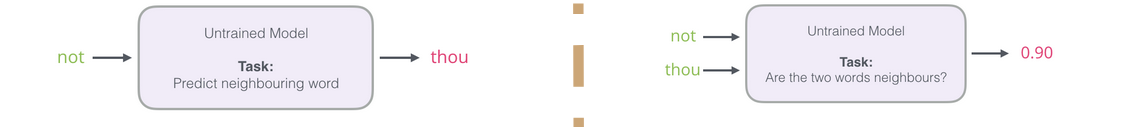
\includegraphics[width=1\textwidth]{images/NLP/24.png}
 \captionsetup{justification=centering,margin=2cm}
 \caption{Comparación Skipgram con distintas funciones de salida: softmax (izquierda) y sigmoide (derecha)\cite{datitos_nlp}.}
 \label{fig:Imagen_NLP_24}
\end{figure}

De esta manera, mediante muestreo negativo pasamos de usar la Fórmula \ref{eq:ecuacion_15_NLP} para calcular la probabilidad de la palabra $w_o$ dada $w_c$ (que representa la probabilidad $P(w^{(t+j)} | w^{(t)}; \theta)$), a utilizar la Fórmula \ref{eq:ecuacion_17_NLP}, la cual calcula la probabilidad de que la salida sea 1, dadas las 2 palabras $w_c$ y $w_o$.  

\begin{equation}\label{eq:ecuacion_17_NLP}
P(D=1 | w_c, w_o) = \sigma (u_{o}^{T} v_c)    \qquad \text{(Ver \cite{NLP_27})}
\end{equation}
\begin{center}
\textit{Probabilidad de que la salida sea 1, dadas $w_o$ y $w_c$  \\ (función de salida sigmoide).}
\end{center}

Reescribimos la fórmula descrita anteriormente para la función sigmoide (Fórmula \ref{eq:ecuacion_8_ANN}) adaptándola a nuestro caso: Fórmula \ref{eq:ecuacion_18_NLP}.

\begin{equation}\label{eq:ecuacion_18_NLP}
\sigma (u_{o}^{T} v_c) = \frac{1}{1 + exp(- (\sigma (u_{o}^{T} v_c)) )}    \qquad \text{(Ver \cite{NLP_27})}
\end{equation}
\begin{center}
\textit{Función sigmoide utilizada.}
\end{center}

En la Figura \ref{fig:Imagen_NLP_25} podemos observar un ejemplo de construcción de datasets para utilizar como entrenamiento: usando como función de salida softmax (parte izquierda) y sigmoide (parte derecha). De esta manera pasamos de tener un dataset donde la entrada y salida son las dos palabras, a uno donde tengamos las dos palabras como features, y la etiqueta “target” que es el valor que debería arrojar el modelo.

\begin{figure}[H]    
 \centering
 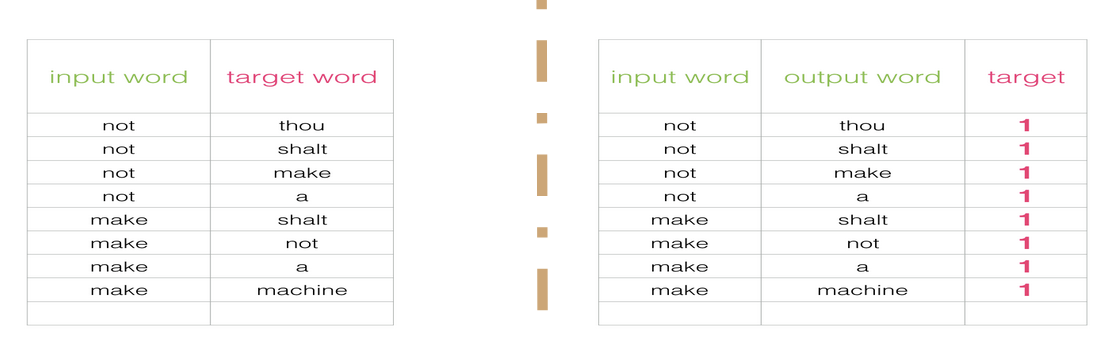
\includegraphics[width=1\textwidth]{images/NLP/25.png}
 \captionsetup{justification=centering,margin=2cm}
 \caption{Armando el datasets para distintas funciones de salida: softmax (izquierda), sigmoide (derecha)\cite{datitos_nlp}.}
 \label{fig:Imagen_NLP_25}
\end{figure}

El problema del dataset descrito anteriormente (utilizando sigmoide) es que los ejemplos son siempre positivos: tenemos dos palabras y la respuesta/salida siempre es 1. Si dejamos todas las etiquetas en 1 el modelo rápidamente va a aprender que prediciendo 1 está en lo correcto y tendrá un 100\% de efectividad. 

Aquí entran los ejemplos negativos (\textit{muestreo negativo}): tenemos que agregar palabras que no vayan juntas para que el modelo aprenda que esas palabras no van juntas. De esta manera, mediante el muestreo negativo (Figura \ref{fig:Imagen_NLP_26}) lo que hacemos es que para cada ejemplo positivo agarramos \textit{palabras al azar} del vocabulario mediante “\textit{random sampling}”\footnote{En el \textit{random sampling} lo más óptimo es agarrar palabras muy improbables de nuestro vocabulario para que nuestro modelo aprenda que no tiene que poner esas palabras.} (como “aaron” y “taco”), las metemos en el dataset y le colocamos etiqueta 0. Es decir, por cada ejemplo positivo estamos metiendo (en este caso) 2 negativos. 

\begin{figure}[H]    
 \centering
 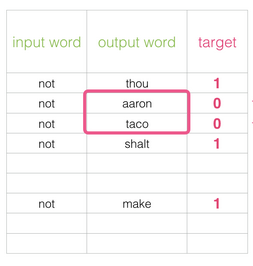
\includegraphics[width=0.3\textwidth]{images/NLP/26.png}
 \captionsetup{justification=centering,margin=3cm}
 \caption{Armando el datasets para función de salida sigmoide usando negative sampling\cite{datitos_nlp}.}
 \label{fig:Imagen_NLP_26}
\end{figure}

¿Cuántas palabras negativas ponemos por cada positiva?: esto es otro \textit{hiper-parámetro} de nuestro modelo Word2vec. 

Con esta optimización, transcribimos la Fórmula \ref{eq:ecuacion_17_NLP} anterior para describir la probabilidad de que la salida sea 1, dadas las 2 palabras $w_c$ y $w_o$, a la Fórmula \ref{eq:ecuacion_19_NLP}.

\begin{equation}\label{eq:ecuacion_19_NLP}
P(w^{(t+j)} | w^{(t)}) = P(D=1 | w^{(t)}, w^{(t+j)})  \prod_{k=1, w_k \sim P(w)}^{K} \; P(D=0 | w^{(t)}, w_k)     \qquad \text{(Ver \cite{NLP_27})}
\end{equation}
\begin{center}
\textit{Probabilidad de que $w^{(t+j)}$ sea palabra de contexto de la palabra central $w^{(t)}$ \\ (función de salida sigmoide y uso de negative samping)}.
\end{center}

Teniendo en cuenta que:
\begin{itemize}
\item $P(D=1 | w^{(t)}, w^{(t+j)})$ es la probabilidad de que la salida sea 1 cuando las dos palabras esten juntas $w^{(t+j)}$ y $w^{(t)}$.
\item $\prod_{k=1, w_k \sim P(w)}^{K} \; P(D=0 | w^{(t)}, w_k)$ es la probabilidad de que la salida sea 0 cuando las dos palabras esten juntas ($w^{(t)}$ y la palabra central $w_k$, que es la que agarramos mediante random sampling). El $K$ en esta ecuación define cuántas palabras negativas tenemos en cuenta. 
\end{itemize}

De esta manera, observamos que la Fórmula \ref{eq:ecuacion_19_NLP}, no depende de todo el vocabulario $V$, como sí sucedía en la Fórmula \ref{eq:ecuacion_15_NLP}. La Fórmula \ref{eq:ecuacion_19_NLP} solo depende de las palabras negativas $w_k$ que metamos: por cada ejemplo vamos a tener que iterar sobre esas $K$ palabras en lugar de iterar sobre todo el diccionario \textit{para calcular la función de pérdida} (Fórmula \ref{eq:ecuacion_11_NLP}). $K$ es mucho menor que el vocabulario $V$: generalmente estamos hablando de 5 a 10 ejemplos negativos por cada positivo, y 10 ya es mucho más pequeño que 1 millón (considerando 1 millón como el tamaño de nuestro vocabulario).

\cleardoublepage

\paragraph{Entrenamiento y función de costo con Sigmoide.}\label{ent_costo_sigmoide}

El ciclo de entrenamiento del modelo Word2vec con función de salida sigmoide y utilizando negative sampling es similar al descrito en la sección \textit{\nameref{ent_costo_softmax}}. La diferencia es que la función de salida es sigmoide en lugar de softmax, y la función de coste $J$ será distinta; el resto de los pasos indicados anteriormente para el entrenamiento son los mismos.

Resumidamente, para realizar el entrenamiento de nuestro modelo Word2vec con función de salida sigmoide y utilizando negative sampling, el primer paso es generar nuestras matrices $W$ y $W'$: Figura \ref{fig:Imagen_NLP_27}. Para esto se generan los 2 vectores que vimos anteriormente ($v_w$ -vector de la palabra central-, y $u_w$ -vector de la palabra de contexto-) por cada palabra de nuestro vocabulario. Con estos vectores se crean dichas matrices: la \textit{matriz de embedding} ($W$) cuando la palabra es la central; y la \textit{matriz de contexto} ($W'$) cuando la palabra es de contexto. Ambas matrices tienen \textit{el mismo tamaño}, por lo que tienen una representación de embedding para cada palabra de nuestro vocabulario. Las filas son las palabras de nuestro vocabulario y las columnas es el tamaño del embedding: otro \textit{hiper-parámetro} de nuestro modelo Word2vec.

\begin{figure}[H]    
 \centering
 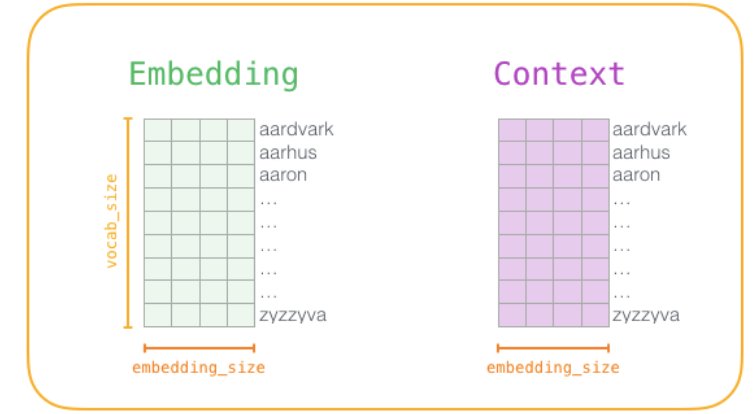
\includegraphics[width=0.7\textwidth]{images/NLP/27.png}
 \captionsetup{justification=centering,margin=2cm}
 \caption{Primer paso entrenamiento Word2vec con función de salida sigmoide y utilizando negative sampling\cite{datitos_nlp}.}
 \label{fig:Imagen_NLP_27}
\end{figure}

Luego, viendo la Figura \ref{fig:Imagen_NLP_28}, observamos que el modelo agarra el primer grupo de palabras (en este caso son 3 filas: una fila es la palabra central junto con la palabra de contexto correcta -thou-, y las otras dos filas son la palabra central junto con las palabras de ejemplo negativo -aaron y taco-). Luego el modelo busca la palabra central en la matriz de embedding junto con todas las de contexto en la matriz de contexto, y las separa. 

\begin{figure}[H]    
 \centering
 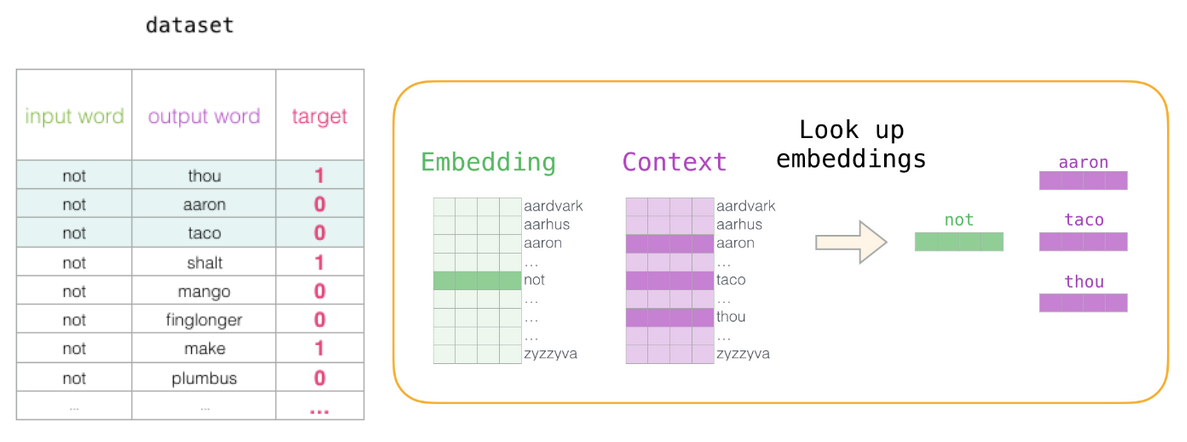
\includegraphics[width=1\textwidth]{images/NLP/28.png}
 \captionsetup{justification=centering,margin=3cm}
 \caption{Obtención de vectores para el cálculo de forward propagation\cite{datitos_nlp}.}
 \label{fig:Imagen_NLP_28}
\end{figure}

Teniendo las etiquetas de estas 3 salidas, lo que hace el modelo es calcular la salida mediante forward propagation, y por último aplicar la función de salida sigmoide. Esto se hace para \textit{todos los ejemplos de entrenamiento}. Una vez finalizado el cálculo de las salidas calculamos el error total, los cuales surgen de la comparación de las salidas de la sigmoide con las etiquetas correspondientes aplicando la función de costo $J$ descrita en la Fórmula \ref{eq:ecuacion_21_NLP}. En esta función de costo observamos que ya no dependemos del tamaño de vocabulario $T$, sino que dependemos de nuestros $k$ ejemplos negativos. Estos errores los usamos para modificar los embeddings de las matrices mediante backpropagation utilizando gradiente descendiente: Figura \ref{fig:Imagen_NLP_29}. 

\begin{equation}\label{eq:ecuacion_21_NLP}
J(\theta) = -log P(w^{(t+j)} | w^{(t)}) = - log \; \sigma (u_{i_{t+j}}^{T} v_{i_{t}}) - \sum_{k=1, w_k \sim P(w)}^{K} \;  log \; \sigma (-u_{h_{k}}^{T} v_{i_{t}})
\end{equation}
\begin{center}
\textit{Función de costo Skipgram (función salida sigmoide y uso de negative sampling})\cite{NLP_27}.
\end{center}

\begin{figure}[H]    
 \centering
 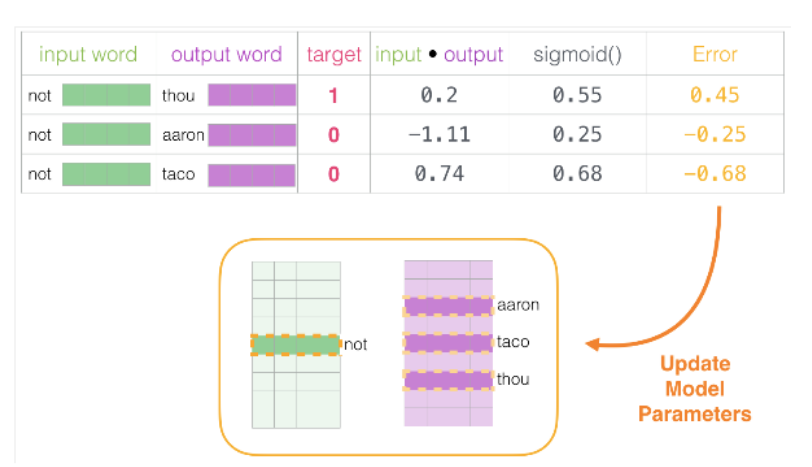
\includegraphics[width=0.8\textwidth]{images/NLP/29.png}
 \caption{Forward y Back propagation\cite{datitos_nlp}.}
 \label{fig:Imagen_NLP_29}
\end{figure}

Mientras se realiza el entrenamiento recorriendo $epoch$ veces nuestro conjunto de datos, los embeddings continúan mejorando su representación para cada una de las palabras. Como mencionamos previamente, estos embeddings son entrenados para que las palabras que siempre están cerca, aparezcan cerca; y por lo tanto en el proceso de entrenamiento el modelo aprenda a codificar estas palabras para que se mantenga el significado de las mismas. 

Una vez que el modelo finalizó el entrenamiento obtendremos nuestras 2 matrices / embeddings listas y lo que se hace es descartar la matriz de contexto $W’$ y \textit{usar la matriz de Embeddings de palabra central $W$ como nuestros embeddings pre-entrenados} para representar a nuestras palabras. 
\\

\paragraph{Desventajas Word2Vec.}\label{desv_word2vec}

Existen tres grandes desventajas de utilizar embeddings obtenidos mediante Word2vec, las cuales describiremos a continuación.

\begin{itemize}
\item La primer limitación\cite{NLP_28} de Word2vec es que sus embeddings \textit{no permiten trabajar con palabras desconocidas por nuestro vocabulario} (palabras \textit{out-of-vocabulary, OVV}). De esta manera, si el embedding no contiene en su vocabulario una palabra, la misma simplemente no se tendrá en cuenta. Esta limitación puede ser solventada utilizando word embeddings obtenidos mediante el modelo \textit{FastText}, el cual es una variante de Word2Vec creada por Facebook que si permite manejar palabras OOV. 

Esta limitación ocurre debido a que Word2vec considera a una palabra como una unidad que no puede ser dividida, mientras que Fasttext considera una palabra como una combinación de sub-palabras. En FastText cada palabra es dividida en n-grams (o “sub-palabras”), los cuales están compuestos por n caracteres. El valor de n define cómo se divide cada palabra en cierto número de n-gramas. Por ejemplo, si $n=3$, “apple” se divide en “app”, “ppl” y “ple”. Una vez que se obtengan los valores vectoriales de las sub-palabras, el valor vectorial de “apple” se convierte en la suma de los valores vectoriales de las sub-palabras. Podemos observar este ejemplo en la Figura \ref{fig:Imagen_NLP_30}.

Esta técnica de entrenamiento permite que utilizando FastText el modelo pueda manejar las palabras OOV. Por ejemplo, consideremos un caso en el que se cuentan en nuestro vocabulario de embedding las palabras “birth” (nacimiento) y “place” (lugar), pero no la palabra “birthplace” (lugar de nacimiento). En Word2vec, al no estar definido el valor del vector “birthplace”, entonces este no se podrá obtener de ninguna forma. En cambio, FastText puede calcular el valor del vector “birthplace” mediante la unión de las subpalabras “birth” y “place”, cuyos vectores si están definidos en nuestro vocabulario. Podemos observar este ejemplo en la Figura \ref{fig:Imagen_NLP_31}.

\begin{figure}[H] %[H] es para que se ubique justo debajo del texto anterior.
\begin{minipage}[b]{0.45\linewidth}
\centering
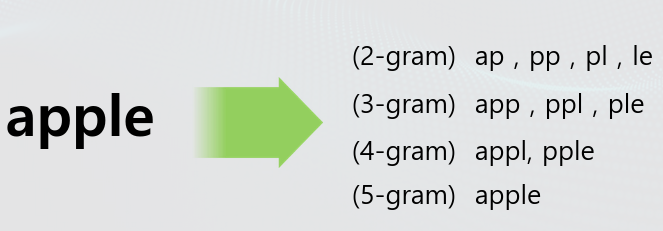
\includegraphics[width=\linewidth]{images/NLP/30.png}
\captionsetup{justification=centering,margin=0.5cm}
\caption{Representación de ‘apple’ mediante FastText\cite{NLP_28}.}
\label{fig:Imagen_NLP_30}
\end{minipage}
\hspace{0.5cm}
\begin{minipage}[b]{0.55\linewidth}
\centering
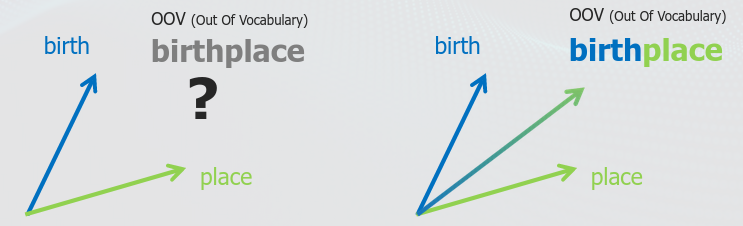
\includegraphics[width=\linewidth]{images/NLP/31.png}
\captionsetup{justification=centering,margin=1cm}
\caption{Word2vec (izquierda) / FastText (derecha)\cite{NLP_28}.}
\label{fig:Imagen_NLP_31}
\end{minipage}
\end{figure}

\item La segunda desventaja\cite{NLP_28} de Word2vec es que \textit{los resultados del embedding no son buenos frente a las palabras que tienen errores tipográficos (datos que presentan ruido)}. Esta limitación también puede ser solventada utilizando FastText. Por ejemplo, consideremos la palabra “apple” y “appple”, que tiene una p adicional como un error tipográfico. En Word2Vec, las dos palabras se consideran palabras completamente separadas. Sin embargo, para FastText, dado que las dos palabras tienen varios n-gramas idénticos, se considerarán palabras similares. Podemos observar este ejemplo en la Figura \ref{fig:Imagen_NLP_32}.

\begin{figure}[H]    
 \centering
 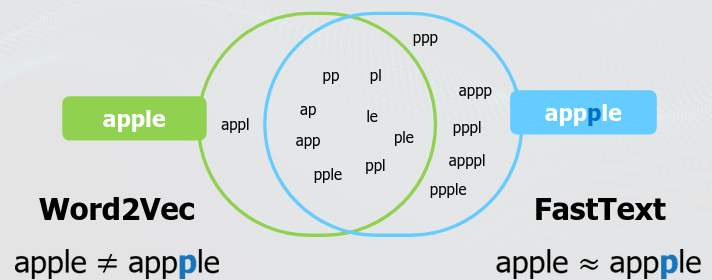
\includegraphics[width=0.8\textwidth]{images/NLP/32.png}
 \caption{Word2vec / FastText\cite{NLP_28}. }
 \label{fig:Imagen_NLP_32}
\end{figure}

\end{itemize}

Como mencionamos previamente, las limitaciones 1 y 2 pueden solventarse utilizando Fasttext. Sin embargo, en nuestra implementación no utilizamos este algoritmo debido a su mayor complejidad de cálculo, ya que para obtener el vector de una palabra en el proceso de entrenamiento tenemos que realizar la \textit{suma de todos los vectores de subpalabras}.

\begin{itemize}

\item La tercer y más importante desventaja de usar embeddings obtenidos mediante Word2Vec\cite{NLP_26}, es que las relaciones construidas entre las palabras son puramente estadísticas y únicamente reflejan la proximidad en un espacio vectorial. Esto es una desventaja, ya que el objetivo de NLP justamente es recrear complejas relaciones que dejen de lado las representaciones estadísticas. De esta manera, muchas veces no nos es útil esta representación para representar palabras que se usan en distintos contextos. Esto es debido a que Word2vec obtiene un embedding que aprende un vector \textbf{fijo} para cada palabra. Aquí el inconveniente es que existen palabras con diversos significados, por ejemplo la palabra ‘queen’ puede ser usada en una oración de piezas de ajedrez o en una oración de tamaños de cama. El vector para la palabra ‘queen’ debería ser distinto dependiendo el contexto, pero en el caso de Word2vec solo existe un único vector ‘queen’ que, en caso de haber sido entrenado con ambas oraciones, supondrá un significado ‘promedio’ entre los 2 contextos. 

\end{itemize}

Esta tercer limitación se puede solventar mediante el uso de modelos de lenguaje más complejos basados en deep learning que permiten obtener embeddings contextuales (como \textit{BERT}, o \textit{ELMo}), permitiendo variar los embeddings dependiendo del contexto. Sin embargo, en nuestra implementación no utilizamos estos modelos debido a que el entrenamiento de los mismos requiere mucho mayor tiempo debido a su mayor complejidad de cálculo\cite{NLP_2}. Otra razón por la cual no utilizamos estos modelos es porque tendríamos que realizar pasos extra para adaptar / transformar la salida de los mismos de modo que sean compatibles con la tarea que queremos realizar a posterior: obtener las similitudes de nuestras palabras en documentos/textos mediante el método Word Mover’s Distance (WMD). Para utilizar WMD como técnica de medición de similitud, lo más simple es utilizar los embeddings obtenidos mediante Word2Vec, como está descrito en el paper de Kusner\cite{NLP_15}.
\\

\subsection{Obtención de las mediciones de similitud entre textos.}\label{med_sim_textos}

El siguiente paso de nuestra aplicación NLP consiste en definir y emplear una métrica de distancia que será utilizada como nuestra medida de similitud entre los vectores numéricos obtenidos del paso anterior (sean mediante BoW, TF-IDF o Embeddings), los cuales representan nuestros textos a comparar.

La medición de similitudes entre textos (text similarity measurement) es uno de los problemas más cruciales del Procesamiento del Lenguaje Natural (NLP). Encontrar similitudes entre documentos se utiliza en varios dominios de NLP, tales como en sistemas de recomendación, information retrieval, automatic question answering, machine translation, dialogue systems, y document matching\cite{similarity_survey}.

Una de las primeras aplicaciones de mediciones de similitud entre textos es quizás el modelo vectorial en la recuperación de información (information retrieval, IR), donde el documento más relevante para una consulta de entrada se determina clasificando los documentos de una colección en órden inverso a su similitud con la consulta dada. Las mediciones de similitud entre textos también se utilizan en sistemas de retroalimentación de relevancia (relevance feedback) y de clasificación de texto (text classification). También se utilizan para tareas de desambiguación del sentido de la palabra (word sense disambiguation) y, más recientemente, para resúmenes de texto (text summarization) y para métodos de evaluación en máquinas de traducción automática (machine translation)\cite{NLP_17_18}.

Para realizar esta tarea de obtener las mediciones de similitud entre nuestros textos utilizaremos dos métodos: uno más convencional (Cosine Similarity, representando previamente nuestros textos con TF-IDF) y un método más actual y novedoso (WMD o Word Mover’s Distance, representando previamente nuestros textos mediante Word embeddings). En la sección \textit{\nameref{cos_y_wmd}} se detallan las razones por las cuales se decidieron elegir estos métodos; las cuales están justificadas en base al análisis realizado en la sección \textit{\nameref{Tecnicas_Simil_textos}}, el cual detalla las numerosas técnicas existentes para obtener similitudes entre textos.

Como mencionamos previamente, una vez que hayamos obtenido estas mediciones de similitud usando estos dos métodos, lo que haremos es combinar dichas mediciones e ingresarlas como entradas a algoritmos de ML (en nuestro caso K-means, y luego KNN) para generar \textit{un modelo de clasificación}. Lo que hará este modelo es, en base a los valores de similitud de los curriculums vitae de nuevos candidatos, lograr clasificar qué tan similares son dichos curriculums vitae con respecto a la descripción de un puesto de IT: similitud escasa, similitud media, similitud alta, similitud muy alta.

A continuación se describirán las técnicas existentes más populares para obtener mediciones de similitud entre textos, haciendo énfasis en las dos técnicas utilizadas en este Proyecto. 
\\

\subsubsection{Maneras de medir la similitud entre textos.}\label{Tecnicas_Simil_textos}

Los textos pueden ser similares de dos maneras: \textit{léxica} y \textit{semánticamente}. Las palabras que componen el texto son similares léxicamente si tienen una secuencia de caracteres similar. En cambio, la similitud semántica determina la similitud entre textos basados en los significados de las palabras que la componen, en lugar de un macheo carácter por carácter. Las palabras son similares semánticamente si tienen algo en común, son opuestas entre sí, se usan de la misma manera, se usan en el mismo contexto y si una es un tipo de otra\cite{NLP_16}.

La similitud de texto no sólo da cuenta de la similitud semántica entre textos, sino que también considera una perspectiva más amplia que analiza las propiedades semánticas compartidas de dos palabras. Por ejemplo, las palabras 'King' y 'Man' pueden estar estrechamente relacionadas entre sí, pero no se consideran semánticamente similares, mientras que las palabras 'King' y ‘Queen' si son semánticamente similares. Así, la similitud semántica puede considerarse como uno de los aspectos de la relación semántica. La relación semántica que incluye la similitud se mide en términos de distancia semántica, que es inversamente proporcional a la relación\cite{similarity_survey}.

Existen muchas métricas para medir similitudes entre textos. Además, existen muchas técnicas para, previamente, representar vectorialmente a nuestros textos. Es por esto que podemos realizar un gran número de combinaciones entre estos métodos de vectorización y uso de métricas de similitud para llevar a cabo nuestra tarea de medición de similitudes entre textos. Esta misma separación fue tomada en cuenta por un estudio publicado en agosto de 2020\cite{similarity_survey}, el cual provee un profundo análisis y conocimiento de las actuales técnicas para medir similitudes entre textos.

En la Figura \ref{fig:Imagen_NLP_33} podemos observar un resumen de dicho estudio, en la cual el cálculo o medición de similitudes entre textos es descrita teniendo en cuenta los dos aspectos mencionados: 
\begin{itemize}
\item \textit{Distancias entre los textos (text distance)}: la cual describe la proximidad semántica de dos palabras de texto desde la perspectiva de la distancia. 
\item \textit{Representaciones de los textos (text representation)}: la cual representa al texto como features o valores numéricos que pueden ser calculados. 
\end{itemize}

Se han propuesto varias medidas y técnicas para medir la similitud semántica durante las últimas décadas. La mayoría de los académicos y estudios previos a este dividen los métodos de medición de similitud de texto basados en corpus de textos (corpus based similarity) y basados en conocimiento (knowledge based similarity)\cite{NLP_16}. Esta clasificación ignora los métodos de cálculo de distancias entre textos, y sólo considera los métodos de representación de textos. 
Es por esto que este estudio\cite{similarity_survey} hace una mayor extensión y subdivisión del sistema de clasificación. Adicionalmente, debido al desarrollo y auge de las redes neuronales en estos últimos años, surgieron varios métodos de representación y cálculos de distancias basándose en estas tecnologías, las cuales fueron agregadas a este estudio y permitieron mejorar enormemente el análisis semántico de las palabras y los textos: como por ejemplo Word Mover’s Distance (WMD), Word2vec, Glove y BERT. 
\\\\

\begin{figure}[H]    
 \centering
 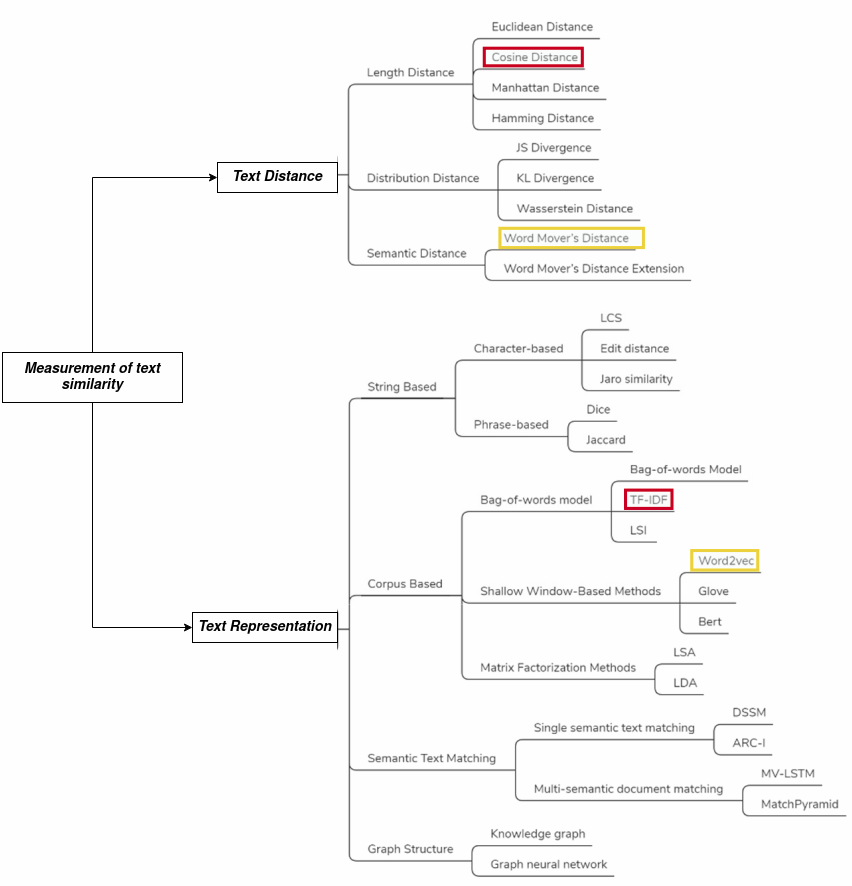
\includegraphics[width=1\textwidth]{images/NLP/33.png}
 \captionsetup{justification=centering,margin=2cm}
 \caption{Medición de similitudes entre textos (remarcadas las técnicas utilizadas en la implementación)\cite{similarity_survey}.}
 \label{fig:Imagen_NLP_33}
\end{figure}

Como podemos observar en la Figura \ref{fig:Imagen_NLP_33} ambos aspectos tienen subdivisiones: la \textit{distancia entre los textos (text distance)} puede ser dividida en distancia de longitud (length distance), distancia de distribución (distribution distance), y distancia semántica (semantic distance); mientras que las \textit{representaciones de los textos (text representation)} pueden ser divididas en representaciones basadas en cadenas de texto (string based), basadas en corpus de texto (corpus based), basadas en macheos/coincidencias semánticas de texto (semantic text matching), y basadas en estructuras de grafos\footnote{Un grafo es un conjunto de objetos llamados vértices o nodos unidos por enlaces llamados aristas o arcos, que permiten representar y estudiar relaciones binarias entre elementos de un conjunto.} (graph structure based). La idea es la misma que expresamos a lo largo de este informe, luego de haber representado los textos vectorialmente se aplican las mediciones de distancias para obtener finalmente las medidas de similitud entre nuestros textos.

A continuación explicaremos más detalladamente en qué consisten estas subdivisiones de \textit{distancia entre los textos (text distance)} y \textit{representaciones de los textos (text representation)}. No entraremos en detalle de cada una de las técnicas involucradas en cada categoría -a excepción de Word Mover’s Distance y Cosine Distance- ya que no entra en los objetivos de este Proyecto, pero si se explicará brevemente en qué consiste cada subdivisión.

Las tres maneras de medir las \textit{distancias entre los textos (text distance)} son \cite{similarity_survey}: 

\begin{enumerate}

\item \textit{De acuerdo a la longitud (Length Distance)}: Tradicionalmente, la similitud entre textos se evaluó midiendo la distancia de acuerdo a la longitud, utilizando de esta forma las características numéricas del texto para calcular la longitud de distancia del texto vectorial. Las 3 distancias más populares de esta categoría son la distancia euclidiana (Euclidean Distance), la distancia del coseno (Cosine Distance) y la distancia de Manhattan (Manhattan Distance). 
Debido a que utilizaremos la distancia del coseno como métrica de similitud entre nuestros textos, la misma está descrita en la sección \textit{\nameref{cosine}}.
Adicionalmente en la sección \textit{\nameref{metrica_dist_emp}} se detallan los cálculos para la distancia euclidiana y distancia de Manhattan.

\item \textit{De acuerdo a la distribución (Distribution Distance)}: Existen dos problemas al usar las distancias basadas en longitud para calcular la similitud. El primero, es que solo es adecuado para problemas simétricos, como Sim (A, B) = Sim (B, A), pero para que la pregunta Q recupere la respuesta A, la similitud correspondiente no es simétrica. En segundo lugar, existe el riesgo de utilizar la longitud y la distancia para juzgar la similitud sin conocer las características estadísticas de los datos\cite{WMD_2}. 
La distancia de distribución se utiliza para comparar si los documentos provienen de la misma distribución, juzgando de esta manera la similitud entre los documentos según dicha distribución. La divergencia JS (JS Divergence) y la divergencia KL (KL Divergence) son actualmente los métodos más populares para investigar la distancia de distribución.

\item \textit{De acuerdo a la semántica de los textos (Semantic distance)}: Cuando no hay una palabra común en el texto, las similitudes obtenidas basándonos en las medidas de distancias basadas en longitud o distribución pueden ser relativamente pequeñas, por lo que podemos considerar calcular la distancia a nivel semántico. La distancia conocida como Word Mover’s Distance (WMD) -también llamada distancia del transportador de palabras- es el principal método utilizado para determinar la distancia semántica\cite{wmd_paper}, el cual será explicado en detalle en la sección \textit{\nameref{wmd}}.

\end{enumerate}

Continuando con las distintas \textit{maneras de representar nuestros textos (Text Representation)}, algo a tener en cuenta es que mientras las representaciones basadas en cadenas de texto (String-Based) y los modelos basados en BoW -pertenecientes a las representaciones basadas en corpus de texto (Corpus-Based)- se basan principalmente en el análisis de \textit{similitud léxica} entre palabras y textos; la \textit{similitud semántica} en cambio, la cual es la que nos interesa abordar, abarca los métodos basados en ventanas poco profundas (Shallow Window-Based Methods) y basados en factorización de matrices (Matrix Factorization Methods) -pertenecientes a las representaciones basadas en corpus de texto (Corpus-Based)-, las representaciones basadas en macheo de macheos/coincidencias semánticas de texto (Semantic Text Matching) y las representaciones basadas en estructuras de grafos (Based on Graph Structure). 

A continuación, explicaremos brevemente las divisiones involucradas en las \textit{maneras de representar nuestros textos (Text Representation)}\cite{similarity_survey}:

\begin{enumerate}

\item \textit{Representaciones basadas en cadenas de texto (String-Based)}:
La ventaja de los métodos basados en cadenas es que son muy fáciles de implementar y los cálculos de similitud que se realizan sobre estos son muy simples de calcular. Las medidas de similitud de cadenas operan en secuencias de cadenas y composición de caracteres que miden la similitud o disimilitud (distancia) entre dos cadenas de texto para una coincidencia o comparación aproximada de cadenas. De acuerdo a la composición de su unidad básica (``basic unit'') se propuso sub-dividir en dos estas representaciones, las cuales explicaremos a continuación.

\begin{itemize}
\item 1.1.\textit{Representaciones basadas en caracteres (Character-Based)}: Un cálculo de similitud basado en caracteres se basa en la similitud entre los caracteres del texto para expresar la similitud entre los textos. Dentro de esta categoría se encuentran tres algoritmos: LCS (Longest Common Substring o subcadena común más larga), distancia de edición (Editing Distance) y similitud de Jaro (Jaro Similarity).
\item 1.2.\textit{Representaciones basadas en frases (Phrase-Based)}: La diferencia entre este método y el método basado en caracteres, es que la unidad básica del método basado en frases es una palabra de frase (phrase word). Los métodos principales son los coeficientes DICE y Jaccard. 
\end{itemize}

\item \textit{Representaciones basadas en corpus de texto (Corpus-Based)}: Existe una diferencia importante entre los métodos basados en corpus y basados en cadenas: el método basado en corpus utiliza la información obtenida de grandes corpus de texto para calcular la similitud del texto; esta información puede ser una característica textual o una probabilidad de co-ocurrencia. Por su parte el enfoque basado en cadenas es una comparación de texto a nivel literal. En los estudios más recientes, el método basado en corpus se mide de tres maneras diferentes, las cuales detallaremos a continuación. 

\begin{itemize}
\item 2.1. \textit{Modelos basados en Bag-of-Words (Bag-of-Words Model)}:  La idea básica del modelo BoW es representar el documento como una combinación de series de palabras sin considerar el órden en que aparecen las palabras en el documento. Los métodos basados en el modelo BoW incluyen principalmente BoW (explicado en la sección \textit{\nameref{bow}}), TF-IDF (explicado en la sección \textit{\nameref{tf_idf}}) y LSI (latent semantic indexing o indexación semántica latente).

\item 2.2. \textit{Métodos basados en ventanas poco profundas (Shallow Window-Based Methods)}: Mejor conocidos como representaciones distribuidas (Distributed Representation), estos métodos difieren de los modelos basados en BoW en un aspecto importante: BoW y TF-IDF no permiten capturar la distancia semántica entre palabras. Utilizando métodos basados en Shallow Windows nos permiten entrenar y obtener vectores de palabras de baja dimensionalidad donde las palabras similares estén más cerca en distancias, resolviendo de esta manera los problemas de la alta dimensionalidad y falta de semántica presente en los modelos basados en BoW. Estas ventajas fueron explicadas en mayor detalle en la sección \textit{\nameref{embedd}}. Un gran número de técnicas fueron desarrolladas para obtener estos vectores de palabras, por nombrar los tres principales métodos presentes en el estudio tenemos a los modelos Word2vec, glove y BERT. Word2vec es el modelo que utilizamos en este Proyecto y fue detallado en la sección \textit{\nameref{word2vec}}.

\item 2.3-\textit{Métodos basados en factorización de matrices (Matrix Factorization Methods)}: Los métodos de factorización matricial para generar representaciones de palabras de baja dimensionalidad tienen raíces que se remontan hasta LSA (Latent Semantic Analysis o análisis semántico latente). Estos métodos utilizan aproximaciones de bajo rango para descomponer grandes matrices que capturan información estadística sobre un corpus. El tipo particular de información capturada por dichas matrices varía según la aplicación. Los avances recientes en los métodos LSA facilitaron la investigación de los métodos LDA (Latent Dirichlet Allocation o asignación de dirichlet latente).
\end{itemize}

\item \textit{Representaciones basadas en macheos/coincidencias semánticas de texto (Semantic Text Matching)}: Como mencionamos previamente, la similitud semántica determina la similitud entre el texto y el documento sobre la base de su significado en lugar de la coincidencia de carácter por carácter. Sobre la base de LSA, estas representaciones son extraídas mediante deep learning y permiten obtener una estructura semántica jerárquica, la cual está embebida en la consulta y el documento. Aquí el texto se codifica para extraer características, por lo que se obtiene una nueva expresión. Estas representaciones pueden ser divididas en Single Semantic Text Matching y Multi-Semantic Document Matching, cuyos métodos principales son visualizados en la Figura \ref{fig:Imagen_NLP_33}.

\item \textit{Representaciones basadas en estructuras de grafos (Graph Structure-Based)}: Recientemente los grafos siendo utilizados como una forma de datos de texto estructurado llamaron la atención de la investigación académica y empresarial. Existen algoritmos basados en grafos para aprender y aplicar distribuciones semánticas en aplicaciones de NLP. La ventaja de la representación basada en grafos y el cálculo de la similitud de textos sobre estas representaciones, radica en que los vínculos (o links) entre los nodos se establecen a través de los bordes (o edges) de las estructuras de grafos para obtener un mejor grado de similitud entre los nodos. Según los diferentes tipos de grafos, principalmente se basan en la representación de grafos de conocimiento (Knowledge Graph) y en la representación de redes neuronales basadas en grafos (Graph Neural Network).
\\
\end{enumerate}

\subsubsection{¿Por qué decidimos utilizar Cosine Similarity y WMD?}\label{cos_y_wmd}

Como observamos en la sección \textit{\nameref{Tecnicas_Simil_textos}}, existen numerosas técnicas para obtener las similitudes de nuestros textos, tanto de medición de distancias como de representación de los textos. En base al análisis anterior, para el sistema desarrollado en este Proyecto se decidió utilizar una combinación entre Cosine Similarity y WMD para realizar la medición de la distancia entre textos. A continuación explicaremos las razones por las cuales optamos por estos métodos.
\begin{itemize}
\item En el caso de \textit{Cosine Similarity}, se utilizó dicha técnica debido a que es una de las más tradicionales y ampliamente utilizadas para medir similitudes entre textos en varias aplicaciones\cite{similarity_survey, cosine_sim_1, cosine_sim_2, cosine_sim_3}.
\item En cambio, \textit{Word Mover’s Distance (WMD)} es una técnica más actual (2015)\cite{wmd_paper} que al momento del estudio publicado el 31 de Agosto del 2020\cite{similarity_survey} es la principal técnica utilizada para la medición semántica de la distancia entre textos.
\end{itemize}

A su vez, se decidieron utilizar las siguientes técnicas para representar vectorialmente los textos a comparar:
\begin{itemize}
\item \textit{Para Cosine Similarity} previamente utilizamos \textit{TF-IDF} para representar vectorialmente nuestros textos. De igual forma esta elección es debido a que TF-IDF es una de las técnicas más tradicionales y ampliamente utilizadas para representar textos y usar en conjunto con Cosine Similarity para medir similitudes entre textos\cite{similarity_survey}. 
\item \textit{Para Word Mover’s Distance (WMD)} previamente utilizamos \textit{Word embeddings} obtenidos de \textit{Word2vec} para representar vectorialmente nuestros textos. Utilizamos el modelo Word2vec para obtener los embeddings y no otro (como por ejemplo Glove, Doc2Vec o BERT)  debido a que en el paper original de WMD\cite{wmd_paper} se utilizan embeddings obtenidos mediante Word2vec, decidiendo de esta manera utilizar la misma base.
\end{itemize}

\cleardoublepage

\subsubsection{Cosine Similarity.}\label{cosine}

Al medir la \textit{similitud del coseno}, en lugar de medir la distancia entre dos puntos -como ocurría en la distancia Euclidiana o distancia Manhattan- esto se transforma a un problema donde se debe medir el coseno del ángulo correspondiente a estos dos puntos -representados como vectores- proyectados en un espacio multidimensional. En la Figura \ref{fig:Imagen_NLP_34} podemos observar que un menor ángulo indica una mayor similitud. Mientras más pequeño sea el ángulo, más parecidos van a ser los vectores. Si el coseno nos da 1 es que son el mismo vector. Si los vectores son ortogonales, el coseno es 0, por lo que estos dos vectores no tendrán relación entre sí. Y cuando el valor nos da muy grande y negativo esto quiere decir que los vectores son opuestos. En nuestra implementación consideramos a estos vectores como los textos que compararemos.

\begin{figure}[H]    
 \centering
 \includegraphics[width=0.9\textwidth]{images/NLP/34.png}
 \caption{Obteniendo similitud del coseno.}
 \label{fig:Imagen_NLP_34}
\end{figure}

De esta manera, considerando $x$ e $y$ como vectores a los cuales queremos calcular su similitud del coseno, su cálculo se obtiene mediante la Fórmula \ref{eq:ecuacion_22_NLP}.

\begin{equation}\label{eq:ecuacion_22_NLP}
CosSim(x,y) = cos(\theta) = \frac{x . y}{ {||x|| \; ||y||} } = \frac{\sum_{i=1}^{n} x_{i} y_{i}}{\sqrt{\sum_{i=1}^{n} x_{i}^{2}} \sqrt{\sum_{i=1}^{n} y_{i}^{2}} }    \qquad \text{(Ver \cite{KNN_Ejemplo})}
\end{equation}
\begin{center}
\textit{Similitud del coseno.}
\end{center}

Donde $x= (x_1,x_2,..., x_n)$, $y = (y_1,y_2,...,y_n)$ y $n$ = dimensiones de los puntos.

Algo a tener en cuenta es que de la \textit{similitud del coseno} deriva la \textit{distancia del coseno}, o también llamada distancia angular, la cual se obtiene sustrayendo la similitud del coseno de 1. Considerando x e y como vectores a los cuales queremos calcular su distancia angular, su cálculo se obtiene mediante la Fórmula \ref{eq:ecuacion_23_NLP}.

\begin{equation}\label{eq:ecuacion_23_NLP}
CosDist(x,y) = 1 - \frac{\sum_{i=1}^{n} x_{i} y_{i}} { \sqrt{\sum_{i=1}^{n} x_{i}^{2}}  \sqrt{\sum_{i=1}^{n} y_{i}^{2}} }     \qquad \text{(Ver \cite{KNN_Ejemplo})}
\end{equation}
\begin{center}
\textit{Distancia del coseno.}
\end{center}

Donde $x= (x_1,x_2,..., x_n)$, $y = (y_1,y_2,...,y_n)$ y $n$ = dimensiones de los puntos.
\\

La similitud del coseno es uno de los principales métodos utilizados para medir la similitud entre dos textos $x$ e $y$. Generalmente calcular la similitud del coseno para medir la similitud entre documentos de texto resulta mucho más eficiente que utilizar la distancia euclidiana para el mismo fin\cite{similarity_survey}.

Como mencionamos previamente, estos textos $x$ e $y$ están representados en forma de vectores. Si utilizamos la representación vectorial mediante el uso de TF-IDF, cada palabra en el texto definirá una dimensión en el espacio vectorial (siendo $x_1, x_2,..., x_n$ las palabras del documento 1; e $y_1, y_2,..., y_n$ las palabras del documento 2) y el valor TF-IDF de cada palabra corresponderá al valor en dicha dimensión. Algo que vale la pena recordar, es que utilizando TF-IDF la limitación que tenemos es que esta representación no cuenta con la habilidad de reconocer si las palabras que se comparan son semánticamente similares. Además, debido a que los valores de TF-IDF son únicamente valores positivos, entonces la similitud del coseno estará en el intervalo [0,1] y el ángulo entre los vectores no podrá ser mayor a 90°, por lo que podremos usar la distancia del coseno (Fórmula \ref{eq:ecuacion_23_NLP}) para obtener nuestra similitud\cite{NLP_19}.

Por ejemplo, teniendo en cuenta la Figura \ref{fig:Imagen_NLP_35} y considerando que $C$, $Q$ y $D$ son nuestros textos a comparar -los cuales están representados en vectores de 2 dimensiones $X1$ y $X2$-, podemos visualizar que calculando la similitud del coseno entre estos documentos, el menor ángulo que obtengamos será entre $Q$ y $D$, por lo que estos serán los documentos más símiles considerando la la similitud del coseno como nuestra métrica de similitud.  

\begin{figure}[H]    
 \centering
 \includegraphics[width=0.5\textwidth]{images/NLP/35.png}
 \caption{Similitud del coseno entre documentos\cite{NLP_19}.}
 \label{fig:Imagen_NLP_35}
\end{figure}

\cleardoublepage

\subsubsection{Word Mover’s Distance (WMD).}\label{wmd}

La distancia conocida como \textit{Word Mover’s Distance (WMD)} -también llamada \textit{distancia del transportador de palabras}- surgió en el año 2015\cite{wmd_paper} y es el principal método utilizado para determinar la similitud semántica entre textos\cite{similarity_survey}. En el cálculo de WMD una menor distancia WMD indica una mayor similitud.
Anteriormente mencionamos que una de las limitaciones de Cosine Similarity era no tener la habilidad de reconocer si las palabras que compara son semánticamente similares. En cambio, WMD al tratarse de un algoritmo más complejo basado en mediciones de distancias entre \textit{word embeddings}, si permite mantener las relaciones semánticas entre las oraciones para obtener las similitudes entre los documentos de texto. De esta forma WMD permite encontrar el costo mínimo necesario para que las palabras (representadas como word embeddings) de un documento “viajen” a la posición de todas las palabras del otro documento intentando encontrar el “vecino más cercano” para cada una de estas palabras. Por lo tanto, las colecciones de texto que comparten muchas palabras semánticamente similares deberían tener distancias más pequeñas que las colecciones de texto con palabras muy diferentes\cite{NLP_21}.

Sobre la base de representar el texto como un espacio vectorial, WMD utiliza el método de EMD (Earth Mover’s Distance, originario en 1998)\cite{WMD_3, WMD_4} para medir la distancia mínima requerida para que una palabra en un texto se mueva hacia una palabra en otro texto en el espacio semántico, y de esta manera minimizar el costo de transportar un texto A a un texto B\cite{WMD_5}. Para calcular esta distancia mínima se utiliza la \textit{distancia euclidiana}. Resumidamente WMD es un método que utiliza la transportación sobre la base de los vectores de palabra (word embeddings)\cite{wmd_paper}.

Veamos un ejemplo\cite{NLP_20}. Si bien Word2vec es un enfoque sofisticado cuando se trata de generar word embeddings de calidad, estos vectores de palabras por sí solos no son suficientes para resolver a la tarea de comparar textos (los cuales están formados por diferentes word embeddings) y obtener la similitud entre ambos. Por ejemplo, consideremos estos dos textos / oraciones: “\textit{My smart home should turn on my favorite music when I come to my home.” y “My smart home shall play my most favored songs when I arrive at my place}”. Vemos que las oraciones transmiten básicamente la misma información. Obteniendo los word embeddings de ambos textos y colocándolos en un espacio de embedding, observaremos que algunos de sus vectores estarán cerca, especialmente si las palabras son símiles (por ejemplo, los pares $<music, songs>$  y  $<come, arrive>$  estarán cerca). La cercanía de los textos / oraciones completas,  por otro lado, no se puede representar solo en el modelo Word2vec. Para superar esta escasez, surgió Word Mover's Distance (WMD) como una medida de distancia basada en palabras (word-based) para textos / oraciones completas. Basado en la creacioń previa de word embeddings (como, por ejemplo, utilizando el modelo Word2vec), la distancia entre dos documentos de texto $A$ y $B$ se describe como la distancia acumulada mínima que las palabras del documento $A$ deben recorrer para coincidir exactamente con la nube de puntos del documento $B$. Con este método, WMD alcanza un alto grado de precisión estando completamente libre de hiper-parámetros y, por lo tanto, siendo fácil de usar.

Tomaremos otro ejemplo\cite{NLP_21} para explicarlo gráfica y matemáticamente. Este es un ejemplo adaptado del paper original de WMD\cite{wmd_paper}. En la Figura \ref{fig:Imagen_NLP_36} vemos un ejemplo de ilustración de las distancias euclidianas entre word embeddings. Algo a tener en cuenta es que en este ejemplo es un espacio vectorial de 2 dimensiones únicamente por motivos ilustrativos, usualmente los vectores de palabras tienen un tamaño de entre 50 a 500 dimensiones.

Cada cantidad (una por flecha) indica la contribución de ese par de palabras a la estadística general de WMD para esos dos documentos. Estas cantidades son el producto de dos números: $c(i,j)$, que es la distancia euclidiana entre las dos palabras en el espacio de embeddings n-dimensional -también llamado 'word travel cost'-, y un término de ponderación/peso $T_{ij}$ que indica cuánto de $i$ en un documento $A$ debe viajar a la palabra $j$ en el otro documento $B$. La contribución de la distancia entre “Chicago” e “Illinois” a WMD entre los documentos 1 y 2 es de $0,18$, mientras que la contribución de la distancia entre “speaks” y “greets” es ligeramente mayor, $0,24$: esto lo podemos visualizar en la Figura \ref{fig:Imagen_NLP_37}, en el cálculo de WMD$(doc1, doc2)$. Vemos que al realizar este cálculo se toma el costo acumulado de mover todas las palabras en el $Documento 1$ a las ubicaciones de las palabras en el $Documento 2$. Esta distancia WMD dió un resultado de 1.07, siendo menor que el resultado obtenido de WMD$(doc3, doc2)$: $1.63$. Esto nos indica que existe una mayor similitud entre los documentos 1 y 2 que entre los documentos 3 y 2. 

\begin{figure}[H]    
 \centering
 \includegraphics[width=0.6\textwidth]{images/NLP/36.png}
 \captionsetup{justification=centering,margin=2cm}
 \caption{Ejemplo de ilustración de las distancias euclidianas entre word embeddings (2 dimensiones)\cite{NLP_21}.}
 \label{fig:Imagen_NLP_36}
\end{figure}

\begin{figure}[H]    
 \centering
 \includegraphics[width=0.5\textwidth]{images/NLP/37.png}
 \captionsetup{justification=centering,margin=2cm}
 \caption{Ejemplo del cálculo de WMD$(d1,d2)$ y WMD$(d3,d2)$\cite{NLP_21}.}
 \label{fig:Imagen_NLP_37}
\end{figure}

Matemáticamente hablando, el algoritmo WMD puede ser descrito como un problema de optimización (Fórmula \ref{eq:ecuacion_24_NLP}), donde se buscan los valores de una matriz T que minimizan “mover” un documento A, a otro documento B. De esta manera el mínimo resultado es la distancia de los dos documentos. 

\begin{equation}\label{eq:ecuacion_24_NLP}
WMD_{ij} = \min_{T\geq0} \sum_{i,j = 1}^{n} T_{ij} c(i,j)      \qquad \text{(Ver \cite{NLP_21})}
\end{equation}
\begin{center}
\textit{Cálculo de WMD.}
\end{center}

Donde:
\begin{itemize}
\item $i$: cada una de las palabras de un documento $A$.
\item $j$: cada una de las palabras de un documento $B$.
\item $T_{ij}$: término de ponderación que indica cuánto de la palabra $i$ en el documento $A$ debe viajar a la palabra $j$ en el otro documento $B$.
\item $c(i,j)$: costo asociado en “viajar” de una palabra a otra. Es la distancia euclidiana entre la palabra $i$ y la palabra $j$, por lo que $c(i,j) = ||x_{i} - x_{j}||_{2}$ \cite{wmd_paper}.

\end{itemize}

\cleardoublepage

\section{Implementación.}\label{5.Implementacion}

Tal como se mencionó en la sección \textit{\nameref{organizacion}}, una vez concluída la etapa de \textit{análisis e investigación}, se debe llevar a cabo la \textit{implementación del sistema}: tanto la implementación del modelo de clasificación KNN, como su integración a un Sistema Web. A continuación se describirán estas dos grandes partes en las cuales se trabajó para obtener nuestro Sistema final. 

\begin{enumerate}
\item Obtención del modelo de clasificación. 

En esta primera parte se obtuvieron y preprocesaron datasets de Curriculum Vitae de distintos candidatos y descripciones de puestos de trabajo de IT publicados por distintas empresas, para luego ser comparados y obtener similitudes entre los textos utilizando las técnicas para medir distancias y obtener dichas similitudes (WMD y Cosine Similarity) y las técnicas de vectorización (TF-IDF y Word embeddings).

Una vez obtenidas estas mediciones de similitud entre los Curriculum Vitae de los candidatos y las descripciones de los puestos laborales de IT, estos valores se utilizaron para alimentar un algoritmo de clustering K-means que a su vez, con sus datos de salida (4 clusters), alimentan a un modelo de clasificación KNN. Finalmente, con este modelo KNN logramos, en base a los valores de similitud de nuevos candidatos, \textbf{clasificar qué tan similares son dichos candidatos con respecto a la descripción de un puesto de IT}: similitud escasa, similitud media, similitud alta, similitud muy alta.

Estos análisis se realizaron en documentos de Jupyter Notebook utilizando Python, y sirvieron para evaluar el comportamiento del modelo de clasificación y los distintos algoritmos de medición de similitudes para luego ser utilizados en la siguiente etapa. \\

\item Integración al Sistema Web. 

Etapa posterior a la primera parte. Una vez observado que los resultados fueron los esperables, lo que se hizo fue reutilizar las funciones que contenian la lógica de los distintos algoritmos utilizados junto con el modelo de clasificación KNN obtenidos previamente en la parte 1, para integrar todo esto en el sistema web. Este sistema web está realizado en Django\footnote{Framework de desarrollo web de código abierto, escrito en Python, que respeta el patrón de diseño conocido como modelo–vista–controlador.}, y cuenta con una base de datos relacional en MySQL\footnote{Sistema de gestión de bases de datos relacionales (RDBMS) de código abierto respaldado por Oracle y basado en el lenguaje de consulta estructurado (SQL).} que contiene la información de los Curiculum Vitae y Puestos que hayan cargado, junto con las mediciones de similitud que hayan sido realizadas. 

De esta manera, nuestro sistema cuenta con una interfaz gráfica que permita al reclutador cargar los Curriculums Vitae de los candidatos y los puestos que tenga disponible, y principalmente obtener un listado con los candidatos más similes a un puesto determinado, ordenados de mayor a menor de acuerdo a esta \textit{similitud}. Dicha \textit{similitud} representa el resultado obtenido de la clasificación por nuestro modelo KNN.

\end{enumerate}

\cleardoublepage

\subsection{Obtención del modelo de clasificación.}\label{5.1.Obtenciondelmodelopredictivo}

\subsubsection{Esquema.}

En la Figura \ref{fig:FlowCoreSystem} podemos ver el procedimiento utilizado para la obtención de nuestro modelo de clasificación. Estas etapas serán explicadas en las secciones posteriores. \\

\begin{figure}[H]    %[H] es para que se ubique justo debajo del texto anterior. 
  \centering
  \includegraphics[width=1\textwidth]{images/flow-core.png} 	%Incluyendo imagen Flow Core.
  \caption{Workflow para la obtención del modelo de clasificación KNN. \\}  
  \label{fig:FlowCoreSystem}
\end{figure}

\subsubsection{Obtención de sets de datos.}\label{obtencion_set_datos}

En primer lugar debemos definir qué es un set o conjunto de datos.
Un set o conjunto de datos es una tabla de una base de datos o, matemáticamente, una matriz estadística de datos. Cada columna de la tabla representa una variable del set de datos; y cada fila representa a un miembro determinado del mismo.

Para este Proyecto utilizamos dos sets de datos que se obtuvieron mediante la recolección de distintos archivos alojados en la Web. Los mismos se encuentran descritos en las secciones \textit{\nameref{cvs}} y \textit{\nameref{puestos_lab}}.

Cabe destacar que estos sets de datos son necesarios para etapas posteriores: tanto para el entrenamiento y obtención de vectores mediante TF-IDF, como para el entrenamiento de Word2vec y obtención de los Word embeddings, y como para su uso en los algoritmos K-means y KNN. El detalle de las porciones de datasets utilizadas para cada método y etapa está detallado en la sección \textit{\nameref{etapas_set_datos}}.

\cleardoublepage

\paragraph{Curriculum Vitae.}\label{cvs}
Los set de datos de Curriculum Vitae de los candidatos se obtuvieron de las siguientes fuentes:

\begin{enumerate}
\item 228 Curriculums en formato docx y posteriormente convertidos a pdf, obtenidos del sitio Kaggle\footnote{\url{https://www.kaggle.com/palaksood97/resume-dataset}}. Estos pdfs son candidatos de la India con experiencia en el rubro de IT. Ver Figura \ref{fig:DS_Cand_1}.
\item 2484 Curriculums en formato CSV, obtenidos del sitio Kagle\footnote{\url{https://www.kaggle.com/snehaanbhawal/resume-dataset}}. Este CSV cuenta con curriculums vitae obtenidos del sitio web de postulación de trabajos 'livecareer.com'. Figura \ref{fig:DS_Cand_2}.
\item 962 Curriculumns en formato CSV, obtenidos del sitio Kaggle\footnote{\url{https://www.kaggle.com/gauravduttakiit/resume-dataset}}. Este CSV cuenta con curriculums vitae repartidos en distintas categorías de IT. Figura \ref{fig:DS_Cand_3}.
\item 10 Curriculums en formato PDF, los cuales los cuales fueron obtenidos como ejemplos mediante una recolección propia de distintos sitios web. Figura \ref{fig:DS_Cand_4}.
\end{enumerate}

\begin{figure}[H] 
 \centering
 \noindent\makebox[\textwidth]{%
 \includegraphics[width=1\textwidth]{images/Implementacion/1-DS_Candidato_1.png}}
 \caption{Ejemplo de una página de un candidato -pdf- (izquierda) y visualización de los 228 candidatos en el Jupyter Notebook -sin preprocesar- (derecha).} 
 \label{fig:DS_Cand_1}
\end{figure}

\begin{figure}[H] 
 \centering
 \noindent\makebox[\textwidth]{%
 \includegraphics[width=0.95\textwidth]{images/Implementacion/2-DS_Candidato_2.png}}
 \caption{Ejemplo de una fila de un candidato -csv- (izquierda) y visualización de los 2484 candidatos en el Jupyter Notebook -sin preprocesar- (derecha).} 
 \label{fig:DS_Cand_2}
\end{figure}

\begin{figure}[H] 
 \centering
 \noindent\makebox[\textwidth]{%
 \includegraphics[width=0.95\textwidth]{images/Implementacion/3-DS_Candidato_3.png}}
 \caption{Ejemplo de una fila de un candidato -csv- y visualización de los 962 candidatos en el Jupyter Notebook -sin preprocesar- (derecha).} 
 \label{fig:DS_Cand_3}
\end{figure}

\begin{figure}[H] 
 \centering
 \noindent\makebox[\textwidth]{%
 \includegraphics[width=0.95\textwidth]{images/Implementacion/4-DS_Candidato_4.png}}
 \caption{Ejemplo de una página de un candidato -pdf- (izquierda) y visualización de los 10 candidatos en el Jupyter Notebook -sin preprocesar- (derecha).} 
 \label{fig:DS_Cand_4}
\end{figure}

\cleardoublepage

\paragraph{Descripciones Puestos Laborales.}\label{puestos_lab}

Los set de datos de descripciones de puestos laborales se obtuvieron de las siguientes fuentes:

\begin{enumerate}
\item 22.000 descripciones en formato CSV; obtenido del sitio Kaggle\footnote{\url{https://www.kaggle.com/PromptCloudHQ/us-technology-jobs-on-dicecom}}. El CSV cuenta con descripciones de puestos obtenidos del sitio web de USA de postulación de trabajos del rubro de IT 'Dice.com'. Ver Figura \ref{fig:DS_Job_1}.
\item 10 descripciones en formato CSV; obtenidas como ejemplos mediante una recolección propia del sitio Indeed\footnote{\url{https://www.indeed.com/q-USA-jobs.html}} para puestos de trabajo de IT. Ver Figura \ref{fig:DS_Job_2}.
\end{enumerate}

\begin{figure}[H] 
 \centering
 \noindent\makebox[\textwidth]{%
 \includegraphics[width=0.95\textwidth]{images/Implementacion/6-DS_Jobs_2.png}}
 \caption{Ejemplo de una fila de una descripción -csv- (izquierda) y visualización de las 22.000 descripciones en el Jupyter Notebook -sin preprocesar- (derecha).} 
 \label{fig:DS_Job_1}
\end{figure}

\begin{figure}[H] 
 \centering
 \noindent\makebox[\textwidth]{%
 \includegraphics[width=0.95\textwidth]{images/Implementacion/5-DS_Jobs_1.png}}
 \caption{Ejemplo de una fila de una descripción -csv- (izquierda) y visualización de las 10 descripciones en el Jupyter Notebook -sin preprocesar- (derecha).} 
 \label{fig:DS_Job_2}
\end{figure}

\cleardoublepage

\subsubsection{Preprocesamiento de textos.}\label{preproc_practica}
Previamente a utilizar las técnicas para medir distancias y obtener similitudes entre textos (WMD y Cosine Similarity) y los algoritmos de aprendizaje (KNN y K-Means) necesitamos que los datos que comparemos e introduzcamos en los algoritmos estén lo más limpios posible; ya que de lo contrario las mismos podrían clasificar o predecir de forma errónea. Este análisis previo sobre los datos debe ser minucioso ya que puede haber valores incoherentes o absurdos.

El procedimiento para el preprocesamiento y limpieza de los Curriculum Vitae y las descripciones de los puestos laborales de IT fue el siguiente:

\begin{enumerate}
\item Eliminación de filas repetidas e innecesarias.
\item Unión los datasets.
\item Limpieza inicial y normalización.
\begin{itemize}
	\item Codificación de nuestros textos a utf-8.
    \item Conversión a minúscula.
    \item Eliminación de datos no relevantes para nuestros análisis (mails, páginas web y common words).
    \item Eliminación de signos de puntuación y caracteres especiales (incluyendo números).
    \item Eliminaación de stop words.
\end{itemize}
\item Aplicación de Tokenización.
\item Aplicación de Lematización.
\item Obtención y uso de bi-gramas.
\end{enumerate}

Si bien en la sección \textit{\nameref{Proces_textos}} se detalla en qué consiste resumidamente cada etapa, a continuación realizaremos un mayor acercamiento con ejemplos visuales de cada una de las mismas.

En el primer paso, \textit{1. Eliminación de filas repetidas e innecesarias}, eliminamos los registros duplicados (\textit{filas repetidas}) de cada uno de los datasets. Además, en algunos casos se tuvieron que eliminar \textit{filas innecesarias}: por ejemplo, para el caso del dataset visualizado en la Figura \ref{fig:DS_Cand_3}, además de trabajos de IT, también este dataset cuenta con candidatos que pertenecen a trabajos de arte, ventas, salud y deporte, ingeniería eléctrica, civil o mecánica, etc. Para nuestro análisis únicamente nos interesan los trabajos relacionados a IT, es por esto que filtramos únicamente las filas con curriculums que pertenezcan a trabajos de IT (los cuales eran, por ejemplo, los pertenecientes a las categorías 'Data Science', 'Web Designing', 'Java Developer', etc.).

\textbf{Debido a esta manipulación y filtrado de datos la cantidad de filas de nuestros datasets se redujo significativamente}. Por ejemplo, para el caso del dataset descrito anteriormente, pasamos de las 962 filas visualizadas en la Figura \ref{fig:DS_Cand_3} a únicamente 97 filas (Figura \ref{fig:DS_Cand_3_sin_dup}). 

\begin{figure}[H] 
 \centering
 \noindent\makebox[\textwidth]{%
 \includegraphics[width=0.5\textwidth]{images/Implementacion/11-962_sin_dup.png}}
 \caption{Dataset de 962 filas iniciales luego de eliminar filas duplicadas e innecesarias.} 
 \label{fig:DS_Cand_3_sin_dup}
\end{figure}

Luego, en el paso \textit{2. Unión los datasets}, lo que se hizo fue unir por un lado los 4 datasets de candidatos, y por el otro los 2 datasets de puestos de IT. De esta manera, en la Figura \ref{fig:final_antes_preproc} podemos observar los tamaños finales de nuestros datasets y sus repectivas columnas. Este paso fue necesario para simplificar la futura aplicación de las respectivas funciones de limpieza de datos.

\begin{figure}[H] 
 \centering
 \noindent\makebox[\textwidth]{%
 \includegraphics[width=1\textwidth]{images/Implementacion/12-Final_antes_preproc.png}}
 \caption{Datasets de candidatos (izquierda) y de puestos de IT (derecha).} 
 \label{fig:final_antes_preproc}
\end{figure}

El siguiente paso, \textit{3. Limpieza inicial y normalización}, consiste en limpiar y normalizar nuestros datos, tanto de los curriculums vitae como de las descripciones de los puestos de IT. Para esto transformamos nuestros textos codificándolos a utf-8, pasamos todas las letras a minúscula y eliminamos datos no relevantes para nuestros análisis (mails, páginas web y common words)\footnote{Las páginas webs y los correos se eliminaron mediante expresiones regulares.}, signos de puntuación, caracteres especiales (paréntesis, comas, puntos, números, etc.) y stop words.

En la Figura \ref{fig:common_text} podemos observar la lista de common words que eliminamos de los textos. Estas common word son palabras que no consideramos necesarias para nuestro análisis: meses y sus abreviaciones, secciones comunes de los curriculums como 'education', 'work experience', etc. 
    
\begin{figure}[H] 
 \centering
 \noindent\makebox[\textwidth]{%
 \includegraphics[width=1\textwidth]{images/Implementacion/9-common_text.png}}
 \caption{Palabras comunes eliminadas de los textos.} 
 \label{fig:common_text}
\end{figure}

Luego aplicamos en conjunto los pasos \textit{4. Aplicación de Tokenización}\footnote{Al tokenizar dividimos los textos en palabras (tokens). En nuestra implementación utilizamos el tokenizador provisto por la libreria NLTK \detokenize{'work_tokenize'}.} y \textit{5. Aplicación de Lematización}\footnote{Como mencionamos anteriormente, algunas palabras con diferentes significados (por ejemplo 'population' y 'populated') pueden tener la misma raíz ('popul'), y si aplicamos \textit{stemming} nos devolverá esta raíz para ambas palabras (algo que sería incorrecto ya que son palabras con significados distintos). Es por esto que en nuestra implementación utilizamos \textit{lemmatization} en lugar de \textit{stemming}: los ‘lemas’ tienen como objetivo transmitir una idea con una palabra real en lugar de una raíz básica (‘stem’) sin un significado definido, corrigiendo el problema de tener dos conceptos diferentes con la misma raíz.}. Como ejemplo visual vamos a tomar como referencia el pdf del candidato de la Figura \ref{fig:DS_Cand_4}. En la Figura \ref{fig:tokens_obt} observamos los tokens obtenidos después de realizar los pasos 3-5 sobre el mismo. 

\begin{figure}[H] 
 \centering
 \noindent\makebox[\textwidth]{%
 \includegraphics[width=1\textwidth]{images/Implementacion/13-Tokens.png}}
 \caption{Candidato luego de aplicar pasos 3-5.} 
 \label{fig:tokens_obt}
\end{figure}

Podemos visualizar algunos lemmas que se obtuvieron, notando mayormente en este caso que las palabras en plural pasaron a su forma/lema singular: 'tools' a 'tool', 'projects' a 'project', etc.

Por último, en la etapa \textit{6. Obtención y uso de bi-gramas}, se decidió asociar 2 palabras que ocurren frecuentemente como 1 sola palabra utilizando bi-grams (como por ejemplo \detokenize{machine_learning}, \detokenize{data_science}, etc.) con el objetivo de enriquecer nuestro vocabulario. Esto nuevamente se aplicó en los textos de ambos datasets. Siguiendo con el ejemplo de la Figura \ref{fig:tokens_obt}, al aplicar bi-grams obtuvimos los tokens visualizados en la Figura \ref{fig:bigrams_obt}.

\begin{figure}[H] 
 \centering
 \noindent\makebox[\textwidth]{%
 \includegraphics[width=1\textwidth]{images/Implementacion/14-bi-grams.png}}
 \caption{Candidato luego de aplicar bi-gramas.} 
 \label{fig:bigrams_obt}
\end{figure}

En las Figuras \ref{fig:Cand_clean} y \ref{fig:Desc_clean} podemos observar el resultado final de los datasets de candidatos y descripciones de puestos de IT respectivamente, una vez que se completó el preprocesamiento de textos (desde el paso 1 al 6).

Podemos observar un gran contraste al compararlo con los mismos datasets antes de pasar por la etapa \textit{3.Limpieza inicial y normalización}: Figura \ref{fig:final_antes_preproc}.

\begin{figure}[H]    
 \centering
 \includegraphics[width=1\textwidth]{images/Implementacion/8-DS_Cand_Clean.png}
 \captionsetup{justification=centering,margin=3cm}
 \caption{Dataset de candidatos luego de realizar el preprocesamiento.}
 \label{fig:Cand_clean}
\end{figure}

\begin{figure}[H]    
 \centering
 \includegraphics[width=1\textwidth]{images/Implementacion/7-DS_Jobs_Clean}
 \captionsetup{justification=centering,margin=3cm}
 \caption{Dataset de descripciones de puestos luego de realizar el preprocesamiento.}
 \label{fig:Desc_clean}
\end{figure}

\cleardoublepage

\subsubsection{Cantidad final del set de datos y su uso en las distintas etapas.}\label{etapas_set_datos}

Una vez realizada la etapa de preprocesamiento y limpieza de datos nos quedaron los siguientes tamaños de nuestros datasets:
\begin{itemize}
\item 624 curriculums vitae de candidatos (en formato pdf y csv). Ver Figura \ref{fig:Cand_clean}.
\item 20593 descripciones de puestos de IT (en formato csv). Ver Figura \ref{fig:Desc_clean}.
\end{itemize}

El total de 624 curriculums vitae de candidatos y 20593 descripciones de puestos de IT que mencionamos previamente, serán utilizados para el entrenamiento y obtención de vectores mediante TF-IDF (para el posterior cálculo de Cosine Similarity) y para el entrenamiento de Word2Vec y obtención de los Word embeddings (para el posterior cálculo de WMD).

Por otro lado, para calcular los valores de Cosine Similarity y WMD, los cuales serán utilizados posteriormente para la aplicación de K-means y KNN, utilizaremos únicamente una porción de nuestros datasets:

1-Para el cálculo de Cosine Similarity y WMD:
\begin{itemize}
\item 101 curriculums vitae de candidatos.
\item 31 descripciones de puestos de IT.
\end{itemize}
\textit{Nota: No obstante, al realizar los cálculos de distancias compararemos cada curriculum vitae con cada Job Description, por lo que obtendremos un dataframe final de \textbf{3131} filas con sus respectivos valores de WMD y Cosine Similarity.}

2-Para el uso de K-means y entrenamiento con KNN (eliminamos un curriculum vitae y una descripción de puesto IT que los utilizamos en '3-'):
\begin{itemize}
\item 100 curriculums vitae de candidatos.
\item 30 descripciones de puestos de IT.
\end{itemize}        
\textit{Nota: como se comentó previamente, nos quedarán \textbf{3000} filas / puntos para usar en K-means y entrenar KNN; llegando a representar estos 3000 puntos en un plano de 2 dimensiones.}

3-Para la clasificación de nuevas muestras mediante KNN:
\begin{itemize}
\item 1 curriculum vitae de candidatos.
\item 1 descripción de puesto de IT.
\end{itemize}
\textit{Nota: como se comentó previamente, nos quedarán 131 filas para clasificar.}

\cleardoublepage

\textbf{¿Por qué utilizamos solo una porción de nuestros datasets?: Esto es debido a los drawbacks de WMD y KNN.}
\begin{itemize}
\item \textit{WMD} posee una alta complejidad en el cálculo de la distancia, teniendo un tiempo de ejecución muy elevado. Como ejemplo, al correrlo localmente, el cálculo de WMD para 3131 filas tardó 7 horas; frente a los 3 segundos que tardó el cálculo de Cosine Similarity para la misma cantidad de filas.
\item \textit{KNN} es una gran opción para datasets pequeños con pocas variables de entrada; pero tiene problemas cuando la cantidad de entradas es muy grande. En grandes dimensiones, los puntos que pueden ser similares pueden tener distancias muy grandes. Además, cada vez que se va a hacer una predicción con KNN, busca al vecino más cercano en el conjunto de entrenamiento completo. Por esto, se debe utilizar un dataset pequeño para que el clasificador KNN complete su ejecución rápidamente.
\end{itemize}
En conclusión, al utilizar solo una porción de nuestros datasets para obtener los distintos cálculos de distancias y entrenar KNN, el cálculo de WMD se podrá realizar en un tiempo finito, y nuestro clasificador KNN funcionará rápida y eficientemente al realizar predicciones.

\cleardoublepage

\subsection{Comparando textos y obteniendo similitudes.}

Una vez teniendo nuestros datos preprocesados (Curriculum Vitae y descripciones de puestos laborales de IT), utilizaremos las técnicas WMD y Cosine Similarity para medir las distancias y obtener las similitudes entre los textos. 

Previamente a utilizar estas técnicas, se debe emplear algun método de vectorización que permita representar las palabras de nuestros textos a un espacio vectorial. De esta forma Cosine Similarity y WMD podrán interpretarlos de la mejor manera. Como mencionamos previamente, como métodos de vectorización se utilizarán TF-IDF y Word embeddings. 

\subsubsection{TF-IDF \& Cosine Similarity.}

Como se mencionó en la sección \textit{\nameref{etapas_set_datos}}, utilizaremos los 624 curriculums vitae de candidatos y 20593 descripciones de puestos de IT para el entrenamiento y obtención de vectores mediante TF-IDF (\textbf{21217} filas en total).

Luego, para el cálculo de las distancias mediante Cosine Similarity utilizaremos 101 curriculums vitae de candidatos y 31 descripciones de puestos de IT (\textbf{3131} filas en total, ya que comparamos cada uno de los curriculums con cada una de las descripciones).

Para el cálculo de TF-IDF y Cosine Similarity se utilizaron clases y métodos provistos por la libreria \textit{Scikit Learn}. Para el caso de TF-IDF se utilizó la clase \textit{TfidfVectorizer}\footnote{Clase \textit{TfidVectorizer}. \url{https://scikit-learn.org/stable/modules/generated/sklearn.feature_extraction.text.TfidfVectorizer.html} (Consultado el 5 de abril de 2022).}, y para el caso de Cosine Similarity se utilizó el método \textit{paired\_cosine\_distances}\footnote{Método \textit{paired\_cosine\_distances}. \url{https://scikit-learn.org/stable/modules/generated/sklearn.metrics.pairwise.paired_cosine_distances.html} (Consultado el 5 de abril de 2022).}.

Para tener una mejor comprensión del procedimiento a realizar se procederá a detallar un ejemplo. En el cuadro de la Imagen \ref{fig:1_TF_IDF} podemos observar el cálculo de valores de score TF-IDF luego de entrenar y aplicarse sobre 3 textos: las descripciones del CV de la Candidata \textit{Karla Lewis} (la cual tiene experiencia sobre trabajos de Data Science) y sobre las descripciones de los puestos \textit{Data Scientist} y \textit{Security Scpecialist}. En este caso nuestro vocabulario resultante fue de 381 palabras (por lo que nuestra matriz resultante tiene la misma cantidad de columnas). 

\begin{figure}[H] 
 \centering
 \includegraphics[width=1\textwidth]{images/implementacion_5/1_TF_IDF.png}
 \captionsetup{justification=centering,margin=3cm}
 \caption{Valores de ejemplo de TF-IDF luego de entrenar y aplicarse sobre 3 documentos / textos.} 
 \label{fig:1_TF_IDF}
\end{figure}

Siguiendo con el ejemplo anterior, una vez que tenemos nuestra matriz TF-IDF lo que hacemos es comparar cada CV con cada Job Description aplicando Similitud del coseno (cuyos cálculos para dos vectores están descritos en la sección \textit{\nameref{cosine}}). En este caso calculamos la similitud del coseno entre los vectores V1 y V2, y entre V1 y V3, dándonos como resultado los valores 0.06 y 0.01 respectivamente: Ver Imagen \ref{fig:2_TF_IDF}.Esto es algo esperable, existiendo mayor score de similitud entre \textit{Karla Lewis} (que trabajó previamente en Data Science) y la posición de \textit{Data Scientist}, que al compararla con la posición de \textit{Security Specialist}. 

\begin{figure}[H] 
 \centering
 \includegraphics[width=1\textwidth]{images/implementacion_5/2_TF_IDF.png}
 \captionsetup{justification=centering,margin=3cm}
 \caption{Obtención de ejemplo de Similitud del Coseno luego de calcular TF-IDF.} 
 \label{fig:2_TF_IDF}
\end{figure}

La diferencia de este ejemplo con nuestro caso, es simplemente que TF-IDF se calcula y se aplica para todo nuestro set completo de CVs y descripciones de trabajo (21.217 documentos / textos en lugar de los 3 documentos / textos del ejemplo anterior). En estos 21.217 textos se encontraron 124.141 tokens / palabras únicas (en lugar de los 381 del ejemplo anterior). Es por esto que nuestra matriz TF-IDF resultante es de tamaño 21.217 x 124.141.

Una vez que obtuvimos esta matriz TF-IDF, se calcula la similitud del coseno para una porción de estos vectores TF-IDF: para los vectores de los primeros 101 CVs y de los primeros 31 puestos de trabajo. De esta manera, finalmente obtenemos el dataset de 3131 filas visualizado en la Imagen \ref{fig:3_TF_IDF}, el cual cuenta en la última columna con el score de similitud del coseno luego de aplicar y calcular TF-IDF entre los 101 CVs y los 31 puestos de trabajo.

\begin{figure}[H] 
 \centering
 \includegraphics[width=1\textwidth]{images/implementacion_5/3_TF_IDF.png}
 \captionsetup{justification=centering,margin=2cm}
 \caption{Obtención final de Similitud del Coseno luego de calcular TF-IDF.} 
 \label{fig:3_TF_IDF}
\end{figure}

\subsubsection{Word embeddings (Word2vec) \& WMD.}\label{Implementacion_word_emb_y_wmd}

Como se mencionó en la sección \textit{\nameref{etapas_set_datos}}, utilizaremos los 624 curriculums vitae de candidatos y 20593 descripciones de puestos de IT para el entrenamiento y obtención de word embeddings mediante Word2vec (\textbf{21217} filas en total).

Luego, para el cálculo de las distancias mediante WMD utilizaremos 101 curriculums vitae de candidatos y 31 descripciones de puestos de IT (\textbf{3131} filas en total, ya que comparamos cada uno de los curriculums con cada una de las descripciones).

En primer lugar se debe obtener la matriz de embeddings, la cual contiene para cada fila el vector word embedding de cada una de las palabras de nuestro vocabulario\footnote{Cabe destacar que nuestro vocabulario es de 124.141 palabras, pero en el modelo de Word2vec omitimos las palabras de nuestros documentos (curriculums de los candidatos y descripciones de los puestos de IT) que tienen menor frecuencia a 2 quedándonos un vocabulario final de 60713 palabras: Ver hiper-parámetro '$min\_count$' en la sección \textit{\nameref{hiper_par_word2vec}}.}. 

Como mencionamos anteriormente, elegimos entrenar nuestros propios word embeddings en lugar de utilizar word embeddings pre-entrenados, ya que verificamos que no existían varias palabras en el vocabulario de dichos embeddings (también llamadas palabras \textit{out-of-vocabulary, OOV}): como por ejemplo, palabras de 2-grams como data\_scientist, $machine\_learning$, $software\_engineer$; o palabras específicas de lenguajes de programación como Python o Java. Por esta razón decidimos entrenar nuestros propios word embeddings utilizando todo el Corpus disponible de nuestros CVs de candidatos y descripciones de puestos de IT. De esta manera se tendrán en cuenta las relaciones entre palabras como $data\_science$, $machine\_learning$ y demás palabras que estén presentes en nuestros CVs o Descripciones de puestos de IT.

Para la obtención de nuestra matriz de embeddings empleamos el modelo de red neuronal Word2vec utilizando la arquitectura Skipgram en conjunto con el método de Muestreo Negativo. Cabe destacar que estos son algunos de los hiper-parámetros de nuestro modelo, los cuales detallaremos en la sección \textit{\nameref{hiper_par_word2vec}}.

Posteriormente a la obtención de los word embeddings se debe calcular WMD, algo que se detallará en la sección \textit{\nameref{calculo_wmd}}.

Para la implementación de Word2Vec y los cálculos de WMD se utilizaron modelos y métodos provistos por la librería \textit{Gensim}. Para la obtención de los Word Embeddings mediante Word2vec se utilizó el módulo \textit{word2vec}\footnote{Módulo \textit{word2vec}. \url{https://radimrehurek.com/gensim/models/word2vec.html}. (Consultado el 5 de abril de 2022).}; mientras que para el cálculo de WMD se utilizó el método \textit{wmdistance} provisto por dicho módulo\footnote{Método \textit{wmdistance}. \url{https://radimrehurek.com/gensim/auto_examples/tutorials/run_wmd.html}. (Consultado el 5 de abril de 2022).}.
\\

\paragraph{Elección de hiper-parámetros Word2vec.}\label{hiper_par_word2vec}

Algo muy importante a tener en cuenta en la construcción de nuestro modelo Word2vec es la elección de los hiper-parámetros\cite{NLP_26}. Estos juegan un rol crucial en la calidad final de la representación de nuestro modelo. A continuación mencionaremos los hiper-parámetros que utilizamos en la implementación en código de nuestro modelo Word2vec mediante la librería Gensim.

En la Imagen \ref{fig:4_Implementacion_Word2vec} podemos observar cada uno de los hiper-parámetros de nuestra implementación de Word2vec, junto con los valores que le colocamos\footnote{La única variable que no es un hiper-parámetro es \textit{sentences}. En \textit{sentences} colocamos el vector \textit{$lista\_corpus\_tokenizado\_final$} el cual contiene todas las palabras de nuestro vocabulario (de todos los documentos: curriculums de candidatos y descripciones de puestos), las cuales serán usadas para el entrenamiento del modelo Word2vec.}.

\begin{figure}[H] 
 \centering
 \includegraphics[width=0.7\textwidth]{images/implementacion_5/4_Implementacion_Word2vec.png}
 \caption{Hiper-parámetros al implementar Word2vec.} 
 \label{fig:4_Implementacion_Word2vec}
\end{figure}

A continuación tomaremos como referencia los nombres de los hiper-parámetros de la Imagen \ref{fig:4_Implementacion_Word2vec} detallando tanto sus significados como la elección de los valores para los mismos mediante Gensim. Contamos con 7 hiper-parámetros propios del modelo Word2vec\cite{Implem_3} (\textit{alpha}, \textit{epochs}, \textit{$vector\_size$}, \textit{window}, \textit{sg}, \textit{hs}, \textit{negative}) y 1 hiper-parámetro adicional por la propia implementación realizada en Gensim (\textit{$min\_count$}), los cuales podemos modificar de acuerdo a nuestra tarea\footnote{Ejemplos de seteos de hiper-parámetros en Gensim. \url{https://radimrehurek.com/gensim/auto_examples/tutorials/run_word2vec.html}. (Consultado el 5 de abril de 2022).}.

\begin{enumerate}

\item \textit{$min\_count$}: hiper-parámetro propio de la implementación de Gensim que nos permite setear la cantidad mínima de apariciones de una palabra para considerarla o no en nuestro vocabulario y posterior entrenamiento. De esta manera, ignora todas las palabras (no las agrega a nuestro vocabulario) cuando la frecuencia de cada palabra es menor a \textit{$min\_count$}. Si queremos añadir todas las palabras en nuestro corpus colocaremos un valor de '1'. Al colocarle un valor de ‘2’ este hiper-parámetro es el responsable de que nuestro vocabulario sea de 60713 palabras en lugar de 124.141 palabras (este sería el caso si \textit{$min\_count$} = 1). Decidimos utilizar un valor mayor a 1 ya que las palabras que aparecen una sola vez es probable que sean errores tipográficos poco interesantes. Además, no existen suficientes datos para realizar un entrenamiento significativo sobre esas palabras, por lo que es mejor ignorarlas.

\item \textit{window}: permite setear el tamaño de la ventana de contexto: ver Imagen \ref{fig:5_Window}.

\begin{figure}[H] 
 \centering
 \includegraphics[width=0.5\textwidth]{images/implementacion_5/5_Window.png}
\captionsetup{justification=centering,margin=2cm}
 \caption{Hiper-parámetro Ventana de Contexto\cite{datitos_nlp}.}
 \label{fig:5_Window}
\end{figure}

Como mencionamos previamente, la ventana de contexto (o Context Window, “C”) es una ventana de tamaño $m$ que podemos colocar en cualquier parte de nuestro corpus de texto, y define qué tan largo o corto tomamos el contexto (palabras de contexto) para realizar el entrenamiento de nuestro modelo y obtener nuestra representación vectorial\cite{NLP_26}. Dicho de otra forma, nos permite controlar el número de palabras que serán consideradas como contexto para representar a una palabra individual ‘target’. Diferentes tamaños de ventana sirven mejor para diferentes tareas\cite{datitos_nlp}:
\begin{itemize}
\item En la práctica se vió que un tamaño de ventana pequeño (2-15) permite construir embeddings donde las puntuaciones más altas de similitud entre dos filas de embeddings indican que las palabras son intercambiables en la frase. Dicho de otra forma, permite encontrar palabras intercambiables, es decir, las palabras que son muy similares en realidad son palabras que son muy intercambiables en una frase, como que están siempre en el mismo lugar en una frase; esto no quiere decir que sean sinónimos, ya que si nos fijamos los antónimos, aunque sean opuestos, generalmente ocupan el mismo lugar en la frase: “esta película es muy mala” y “esta película es muy buena”, podemos reemplazar “mala” por “buena” y la frase sigue teniendo sentido aunque no quieran decir lo mismo). En conclusión, con una ventana pequeña logramos que solo se fije en lo que ocurre exactamente alrededor de las palabras. 
\item Los tamaños de ventana más grandes (15-50, o incluso más) producen embeddings donde la similitud es más indicativa de la relación de las palabras. Dicho de otra forma, permiten analizar más frases que utilizando un tamaño de ventana pequeño. Siguiendo con el ejemplo anterior, la frase “esta película es muy buena” seguramente va a estar asociada a otras frases anteriores o siguientes que quizás sigan alabando a la película; y la frase “esta película es muy mala” generalmente va a estar rodeada de otras frases con críticas a la película. De esta manera, ahí el modelo aprendería que “mala” y “buena”, aunque estén rodeadas de las mismas palabras, generalmente tienen otro significado. 
\end{itemize}

Otros estudios\cite{Implem_1,Implem_2} encontraron que generalmente se utilizan ventanas grandes al entrenar sobre textos con oraciones largas que contienen estructuras de cláusulas complejas (por ejemplo, literatura biomédica). Además, se demostró que el tamaño de la ventana influye en los tipos de semántica de palabras que captura el modelo: un tamaño de ventana más grande permite capturar información de tópicos / dominio de las palabras: ¿que otras palabras son usadas en tópicos / dominios similares?; en cambio, un tamaño de ventana más pequeño permite capturar más acerca de la funcionalidad de la palabra en sí: ¿qué otras palabras son funcionalmente similares?. Este último caso es mejor, por ejemplo, para encontrar sinónimos de palabras.

En nuestro caso le colocamos a esta variable 15. De esta manera el modelo al entrenar tomará 15 palabras de contexto a la izquierda y otras 15 a la derecha de la palabra target. Se decidió tomar 15 por ser un valor “intermedio” entre las ventanas de tamaño pequeño y grande, y así obtener un balance entre las ventajas de poder capturar tanto los tópicos de las palabras como la funcionalidad de la misma. 

\item \textit{$vector\_size$}: es lo que se conoce como dimensionalidad. Representa el tamaño / dimensión de nuestros words embeddings resultantes (o el tamaño / número de neuronas de la capa oculta). Dicho de otra forma es el número de dimensiones (N) del espacio N-dimensional en donde Wor2vec mapea sus palabras. 

Grandes valores de dimensionalidad requieren más datos de entrenamiento, pero pueden producir mejores modelos (con mayor accuracy) al poder capturar mayor información de las palabras. Lo negativo de usar grandes valores de dimensionalidad es que su entrenamiento es más costoso computacionalmente\cite{Implem_2}. Generalmente se usa un valor de 100 o 50\cite{NLP_26}. En nuestro caso utilizamos su valor por defecto (100) ya que no queremos obtener word embeddings muy extensos debido a su futuro uso en WMD (cuyos cálculos requieren mucho tiempo de procesamiento, y más aún si tenemos word embeddings de grandes dimensiones).  

\item \textit{sg}: indica el algoritmo/modelo de entrenamiento que se utilizará (CBoW o Skip-gram). El valor por defecto en Gensim es 0 (lo que significa que se usará CBOW); pero como nosotros utilizaremos Skip Gram colocamos este valor en 1.

Elegimos SKip-Gram sobre CBOW por lo mencionado en la sección \textit{\nameref{cbow_vs_skip}}: nuestro dataset de entrenamiento no es muy grande (nuestro vocabulario consiste en 60713 palabras) y necesitamos utilizar esta arquitectura que funciona mejor para pocos datos. Además, otro punto a favor de Skipgram es que {nos permite representar mejor palabras “raras” o infrecuentes}, y esto es una ventaja en IT ya que cada vez más cantidad de lenguajes y tecnologías van apareciendo, por lo que aunque una palabra aparezca pocas veces en nuestros corpus de texto, hay que tenerlas en cuenta y tratar de representarlas lo mejor posible.

\item \textit{hs}: si el valor es 0 (como en nuestro caso) indica que se utiliza Negative Sampling como optimización para entrenar a nuestro modelo: explicado en la sección \textit{\nameref{neg_samp}}.

\item \textit{negative}: especifica el número de muestras negativas (cuántas palabras / muestras negativas agregamos al dataset por cada palabra / muestra positiva para el proceso de entrenamiento): ver Imagen \ref{fig:6_Neg_samples}.

\begin{figure}[H] 
 \centering
 \includegraphics[width=0.7\textwidth]{images/implementacion_5/6_Neg_samples.png}
\captionsetup{justification=centering,margin=2cm}
 \caption{Hiper-parámetro Número de muestras negativas.\cite{datitos_nlp}.}
 \label{fig:6_Neg_samples}
\end{figure}

Este hiper-parámetro se elige de acuerdo a la cantidad de datos que tengamos\cite{datitos_nlp}:
\begin{itemize}
\item Si tenemos muchos datos no hace falta que metamos tantos ejemplos negativos por cada uno de los positivos. En cambio, si tenemos pocos datos podemos utilizar los ejemplos negativos para tener un dataset más grande y ayudar a nuestro modelo a que aprenda mejor. 
\item El paper original de Word2vec\cite{NLP_11} prescribe 5-20 como un buen número de muestras negativas. También establece que 2-5 parece ser suficiente cuando tiene un conjunto de datos lo suficientemente grande.
\end{itemize}

El valor por defecto en Gensim es 5, pero en nuestra implementación le colocamos un valor de 10. Esto es debido a que nuestro vocabulario no es tan grande, y es mejor agrandar nuestro dataset de entrenamiento colocando más ejemplos.

\item \textit{alpha}: Este es uno de los hiper-parámetros más comunes que ajustamos al implementar redes neuronales artificiales. Como Word2vec es un modelo de red neuronal, también podemos modificar este hiper-parámetro. alpha hace referencia al learning rate (o tasa de aprendizaje), el cual detallamos en la sección \textit{\nameref{hiper_n}}. Seteamos este valor en 0.025, su valor por defecto en la implementación de Gensim.

\item \textit{epochs}: Este es otro de los hiper-parámetros más comunes en redes neuronales artificiales. Como mencionamos anteriormente, cada epoch en una ANN representa una iteración sobre nuestros datos de entrenamiento / corpus de texto completo. Esta iteración incluye el cálculo de los forward propagation y back propagation correspondientes. Seteamos este valor en 5, su valor por defecto en la implementación de Gensim.

\end{enumerate}

Una vez definidos los hiper-parámetros de nuestro modelo Word2vec, se debe entrenar al mismo con nuestro vocabulario de 60.713 palabras/tokens. Este entrenamiento en la implementación se realiza al correr el código explicado anteriormente en la Imagen \ref{fig:4_Implementacion_Word2vec}. El proceso de entrenamiento que sigue nuestro modelo fue explicado en la sección \textit{\nameref{ent_costo_sigmoide}}. Una vez entrenado nuestro modelo tendremos para cada una de las 60.713 palabras que componen nuestro vocabulario, un word embedding de 100 dimensiones que la representa y que nos permitirá realizar los futuros cálculos de WMD. 

\cleardoublepage

\paragraph{Word Mover's Distance (WMD).}\label{calculo_wmd}

Una vez obtenido los word embeddings de nuestros documentos aplicaremos WMD para obtener otra medida de similitud (además de la calculada previamente con TF-IDF \& Cosine Similarity) entre los candidatos y los puestos.

Para ello primero se debe armar un vector para cada uno de los documentos a comparar (para los 101 CVs y 31 descripciones de puestos de trabajo) que contendrá para cada posición (para cada palabra del documento), -y si es que la palabra pertenece al vocabulario-, una referencia al vector word embedding correspondiente de la matriz de word embeddings calculada previamente. Este paso lo hace internamente la implementación de WMD de Gensim.

Posteriormente estos vectores se utilizan para poder aplicar WMD entre cada uno de los CVs y cada una de las posiciones de trabajo. De esta manera anexaremos el resultado de WMD al dataset obtenido anteriormente en la Imagen \ref{fig:3_TF_IDF}, quedándonos finalmente como la Imagen \ref{fig:7_Calculo_WMD}.

\begin{figure}[H] 
 \centering
 \includegraphics[width=1\textwidth]{images/implementacion_5/7_Calculo_WMD.png}
\captionsetup{justification=centering,margin=3cm}
 \caption{Obtención final de WMD.} 
 \label{fig:7_Calculo_WMD}
\end{figure}

\cleardoublepage

Por ejemplo, para la Candidata de la primer fila de la Imagen \ref{fig:7_Calculo_WMD} (\textit{Karla Lewis}), su vector resultante será: \textit{[word embedding de ‘$data\_scientist$’, word embedding de ‘brooklyn’, word embedding de ‘ny’, word embedding de ‘$data\_scientist$’, (...)]}. 

En la Imagen \ref{fig:8_Word_emb} podemos observar la representación del word embedding ‘$data\_scientist$’, el cual tiene como mencionamos previamente una dimensión de 100. 

\begin{figure}[H] 
 \centering
 \includegraphics[width=0.7\textwidth]{images/implementacion_5/8_Word_emb.png}
\captionsetup{justification=centering,margin=3cm}
 \caption{Word embedding del 2-gram ‘$data\_scientist$’.} 
 \label{fig:8_Word_emb}
\end{figure}

En cambio, para la descripción de trabajo de la primera fila (\textit{Data Scientist}) el vector resultante sería: \textit{[word embedding de ‘$master\_degree$', word embedding de ‘stem‘, word embedding de ‘field‘, word embedding de ‘$including\_limited$‘, (...)]}. 

De dicha forma se puede calcular el WMD para esta Candidata y Descripción de trabajo utilizando estos vectores y los word embeddings de sus palabras\footnote{El cálculo de WMD que se realiza entre 2 vectores fue descrito en la sección \textit{\nameref{wmd}}.}, dándonos como resultado una medida de similitud entre los mismos: visto previamente en la Imagen \ref{fig:7_Calculo_WMD}.

\cleardoublepage

\paragraph{Observaciones valores de Cosine Similarity y WMD.}\label{Obs_cos_y_wmd}

A continuación observaremos algunos ejemplos de los valores de Cosine Similarity y WMD obtenidos para un candidato y descripción en particular, con el objetivo de corroborar que los candidatos posean altos valores de similitud en los puestos donde hayan tenido mayor experiencia y/o donde posean los skills que, a priori, sean los esperables para esa posición.

Tomaremos como ejemplo al candidato \textit{$MLEngineer\_Bradly\_Johnston$}, el cual tiene experiencia previa en varios puestos de Machine Learning y skills de esta área de conocimiento, por lo que a priori es esperable que tenga mayor similitud con puestos de Machine Learning o Data Science. 

En la Imagen \ref{fig:Valores_para_Bradly_Johnson} podemos visualizar un TOP 5 de las descripciones de puestos más y menos similares al Candidato \textit{$MLEngineer\_Bradly\_Johnston$} de acuerdo a nuestras métricas (WMD y TF-IDF \& Cosine).
\\

\begin{figure}[H] 
 \centering
 \includegraphics[width=1\textwidth]{images/implementacion_5/Valores_para_Bradly_Johnson.png}
 \captionsetup{justification=centering,margin=2cm}
 \caption{Posiciones más y menos similares para el Candidato \textit{$MLEngineer\_Bradly\_Johnston$} de acuerdo a nuestras métricas (TF-IDF \& Cosine a la izquierda y WMD a la derecha).} 
 \label{fig:Valores_para_Bradly_Johnson}
\end{figure}

Observamos similares resultados al aplicar tanto para la métrica WMD como TF-IDF \& Cosine Similarity: altos valores de similitud para los puestos \textit{Machine Learning Engineer 2}, \textit{Machine Learning Engineer}, \textit{Data Scientist}, \textit{Data Scientist 2}. Esto como mencionamos previamente, es algo esperable. Además, observamos bajos valores para puestos que no están relacionados a Machine Learning, como por ejemplo \textit{SAP FICO Architect}, \textit{Test Lead / Test Manager}, \textit{DevOps Engineer}, \textit{Project Manager}, etc. Esto también es algo esperable.

\cleardoublepage

Ahora, tomaremos como ejemplo al puesto \textit{Security Specialist 2}. A priori es esperable que este puesto tenga mayor similitud con los CVs de los candidatos que hayan trabajado previamente o tengan skills para el área de seguridad informática. 

En la Imagen \ref{fig:Valores_para_security_spec_2} podemos visualizar un TOP 5 de los CVs de Candidatos más similares al puesto \textit{Security Specialist 2} de acuerdo a nuestras métricas (WMD y TF-IDF \& Cosine).

\begin{figure}[H] 
 \centering
 \includegraphics[width=1\textwidth]{images/implementacion_5/Valores_para_security_spec_2.png}
 \captionsetup{justification=centering,margin=2cm}
 \caption{CVs de Candidatos más similares para el la descripción del puesto \textit{Security Specialist 2} de acuerdo a nuestras métricas (TF-IDF \& Cosine a la izquierda y WMD a la derecha).} 
 \label{fig:Valores_para_security_spec_2}
\end{figure}

Nuevamente se corrobora con este ejemplo nuestra suposición inicial: los curriculums de los candidatos que tienen expertise en seguridad informática (como \textit{Ahmed Wayne} y \textit{Denis Banik}) tienen mayor similitud con el puesto \textit{Security Specialist 2}.

\cleardoublepage

\subsection{Armado del modelo de clasificación KNN.}\label{IMP_Modelo_clasificacion_KNN}

Una vez obtenidas nuestras mediciones de similitud (tanto de TF-IDF \& Cosine Similarity como de WMD) entre nuestras 3131 combinaciones de Curriculum Vitae de candidatos y las descripciones de los puestos laborales de IT, tenemos que encontrar alguna manera de utilizar estas mediciones en conjunto: para esto utilizamos KNN en conjunto con K-means.

De esta manera estos valores de similitud funcionarán como features alimentando al algoritmo de clustering K-means, el cual a su vez con sus datos de salida (4 clusters), alimentará a un modelo de clasificación KNN. Finalmente, con este modelo KNN lograremos, en base a los valores de similitud de nuevos candidatos, clasificar qué tan similares son dichos candidatos con respecto a la descripción de un puesto de IT: similitud escasa, similitud media, similitud alta, similitud muy alta.

Para la implementación de K-means y KNN se utilizaron métodos y clases provistas por la librería \textit{Scikit Learn}. Para el caso de K-means se utilizó la Clase \textit{KMeans}\footnote{Clase \textit{KMeans}. \url{https://scikit-learn.org/stable/modules/generated/sklearn.cluster.KMeans.html} (Consultado el 5 de abril de 2022).}, y para el caso de KNN se utilizó la Clase \textit{KNeighborsClassifier}\footnote{Clase \textit{KNeighborsClassifier}. \url{https://scikit-learn.org/stable/modules/generated/sklearn.neighbors.KNeighborsClassifier.html} (Consultado el 5 de abril de 2022).} junto al método \textit{$cross\_val\_score$}\footnote{Método \textit{$cross\_val\_score$}. \url{https://scikit-learn.org/stable/modules/generated/sklearn.model_selection.cross_val_score.html} (Consultado el 5 de abril de 2022).} para realizar la evaluación mediante cross-validation. \\

\subsubsection{Preparación de los datos.}\label{prep_datosd}

Previamente a utilizar K-means y KNN vamos a eliminar de nuestro dataset obtenido en \ref{fig:7_Calculo_WMD} 1 Curriculum Vitae de un candidato y 1 descripción de puesto laboral (que representan un total de 131 filas del dataset). Estos datos los utilizaremos en la sección \textit{\nameref{5.4.Predicciondenuevasmuestrasyresultadosobtenidos}} para realizar predicciones mediante KNN utilizando dichos Candidatos y Descripciones de Puestos que tienen los valores de WMD y Cosine Similarity calculados. Cabe destacar que esta no es una división de datos de entrenamiento y datos de evaluación, esta es realizada en la sección \textit{\nameref{imp_knn}} utilizando Cross Validation. Esta división se realizó únicamente para simular una predicción para nuevos ejemplos (1 CV y 1 puesto) ya teniendo nuestro modelo de KNN entrenado y evaluado, y analizar estos resultados. 

\cleardoublepage

De esta manera nos quedarán los siguientes datasets\footnote{Adicionalmente nos quedamos únicamente con las columnas necesarias (‘Candidate\_Name’, ‘Job\_Title’, ‘tfidf\_cosine’ y ‘WMD’) eliminando del dataset de la Imagen \ref{fig:7_Calculo_WMD} las columnas que no nos sirven más (‘clean\_Content\_CV’, ‘tokens\_Content\_CV’, ‘clean\_Job\_Description’ y ‘tokens\_Job\_Description’)}:

\begin{itemize}

\item Dataset de 131 filas / puntos para realizar la clasificación de nuevas muestras mencionada previamente: Imagen \ref{fig:eliminacion_hcm_2_y_denis}. Este dataset está formado por las 101 filas correspondientes a la posición \textit{HCM Consultant 2} y las 30 filas correspondientes al candidato \textit{Denis Banik}, las cuales fueron eliminadas del dataset que se utilizará en K-means.

\end{itemize}

\begin{figure}[H]   
\centering
\includegraphics[width=1\textwidth]{images/implementacion_5/eliminacion_hcm_2_y_denis.png}
\caption{Dataset de 131 filas / puntos para realizar la clasificación de nuevas muestras: 101 filas referentes a la posición \textit{HCM Consultant 2} (izquierda) y 30 filas referentes al candidato \textit{Denis Banik} (derecha).}
\label{fig:eliminacion_hcm_2_y_denis}
\end{figure}

\begin{itemize}

\item Dataset de 3000 filas / puntos para utilizar en K-means y KNN: Imagen \ref{fig:dataset_kmeans_knn_final}.

\begin{figure}[H]   
\centering
\includegraphics[width=0.7\textwidth]{images/implementacion_5/dataset_kmeans_knn_final.png}
\caption{Dataset de 3000 filas / puntos para utilizar en K-means y KNN.}
\label{fig:dataset_kmeans_knn_final}
\end{figure}

\end{itemize}

\cleardoublepage

\subsubsection{K-means.}\label{imp_kmeans}

Como mencionamos previamente en la sección \textit{\nameref{k_means_3_4}}, K-means es un algoritmo de clustering que nos sirve para dividir nuestros datos (los cuales no tienen etiquetas) en grupos / clusters. Este algoritmo cuenta con un único hiper-parámetro que debemos definir previamente, el cual es k, o número de clusters.

Como detallamos en la sección \textit{\nameref{limit_kmeans}}, este algoritmo tiene 3 principales limitaciones: los outliers, la determinación del hiper-parámetro k y la inicialización de los centroides. Estos problemas fueron resueltos en nuestra implementación, la cual se detalla a continuación. 

Como primera medida, para el problema de los outliers lo que se hizo es aplicar un pre-procesamiento de datos adicional (que incluye una eliminación de dichos outliers) previamente a utilizar los valores de las métricas de similitud en k-means. 

Inicialmente realizamos un gráfico de dispersión tomando como dimensiones / features a las columnas correspondiente al valor de WMD y el valor de Cosine Similarity (\textit{WMD} que será nuestro eje Y, y \textit{$tfidf\_cosine$} que será nuestro eje X), para visualizar la disposición de nuestros puntos de datos en dos dimensiones: Imagen \ref{fig:dispersion}.

\begin{figure}[H]   
\centering
\includegraphics[width=0.7\textwidth]{images/implementacion_5/dispersion.png}
\captionsetup{justification=centering,margin=2cm}
\caption{Gráfico de dispersión con nuestros valores de similitud como dimensiones.}
\label{fig:dispersion}
\end{figure}

Visualizando el gráfico podemos detectar a simple vista que hay valores que se escapan del “grupo medio”: estos son nuestros outliers, los cuales eliminaremos para que no perjudique al aprendizaje del modelo de ML posterior (KNN). Para eliminarlos vamos a aplicar un límite / condición que filtre los puntos que tengan un Cosine Similarity (eje x) mayor a 0.26. De esta manera se eliminan 7 puntos de datos de nuestro dataset, quedándonos 2993 filas: ver Imagen \ref{fig:detec_elim_outliers}.

\begin{figure}[H]   
\centering
\includegraphics[width=1\textwidth]{images/implementacion_5/detec_elim_outliers.png}
\caption{Detección (izquierda) y eliminación (derecha) de outliers.}
\label{fig:detec_elim_outliers}
\end{figure}

Nuestro próximo paso es determinar el número de k clusters (nuestra segunda problemática en k-means). Para esto aplicamos el \textit{método del codo} (o \textit{elbow method}) explicado en la sección \textit{\nameref{Elbow_Met}}, graficando la Inertia\footnote{Recordando lo visto anteriormente, Inertia es la distancia entre cada punto del cluster y el centroide que tiene asignado, la cual se busca minimizar en K-means. A este criterio de Inertia también se lo considera como la función de coste J en K-means.} en función de k. De esta manera iteramos valores de k desde 1 a 9 y calculamos los valores de Inertia para cada valor de k dentro de ese rango, obteniendo el gráfico de la Figura \ref{fig:elbow_method_inertia}.

\begin{figure}[H]   
\centering
\includegraphics[width=0.6\textwidth]{images/implementacion_5/elbow_method_inertia.png}
\caption{Método del codo usando Inertia.}
\label{fig:elbow_method_inertia}
\end{figure}

Viendo este gráfico concluimos que, para nuestros datos, el punto “del codo” está en k=4, siendo 4 nuestro k óptimo. A partir de k=4 la Inertia comienza a disminuir de forma lineal, o dicho de otra forma, después de k=4, el cambio en la disminución del valor de la Inertia no es significativo. 

\cleardoublepage

Una vez obtenido nuestro k óptimo, pasaremos a calcular y asignar los centroides para dichos clusters. En la Imagen \ref{fig:codigo_k-means} podemos observar la implementación en código mediante la librería \textit{Sklearn} para el cálculo de la ubicación de los centroides en k-means. Aquí vemos que se define \textit{init = ‘k-means ++’}, lo que quiere decir que se utiliza k-means ++ como método de inicialización de nuestros centroides. K-means ++ es uno de los métodos estándar de inicialización, el cual fue detallado en la sección \textit{\nameref{k_means_plus_plus}}. Utilizando este método logramos una asignación de centroides más espaciada, solucionando la tercer y última limitación / problema de k-means: la inicialización de los centroides.

\begin{figure}[H]   
\centering
\includegraphics[width=0.9\textwidth]{images/implementacion_5/codigo_k-means.png}
\captionsetup{justification=centering,margin=3cm}
\caption{Código K-means y obtención de las coordenadas de los centroides.}
\label{fig:codigo_k-means}
\end{figure}

En la Imagen \ref{fig:final_groups} podemos observar como quedó la distribución de los centroides en nuestros puntos de datos (izquierda) y como quedó la asignación de los labels para los cuatro clusters (derecha). 

\begin{figure}[H]   
\centering
\includegraphics[width=1\textwidth]{images/implementacion_5/final_groups.png}
\captionsetup{justification=centering,margin=2cm}
\caption{Distribución de centroides (izquierda) y asignación final de los clusters (derecha).}
\label{fig:final_groups}
\end{figure}

De esta manera, los clusters / grupos obtenidos expresan lo siguiente:
\begin{itemize}
\item Cluster 1: un punto que pertenezca a este cluster indica que existe un nivel bajo de similitud entre el Curriculum Vitae candidato y el la descripción del puesto.
\item Cluster 2: indica un nivel medio de similitud.
\item Cluster 3: indica un nivel alto de similitud.
\item Cluster 4: indica un nivel muy alto de similitud. 
\end{itemize}

Quedándonos como dataset final que utilizaremos en KNN el visualizado en la Imagen \ref{fig:to_knn}.

\begin{figure}[H]   
\centering
\includegraphics[width=0.8\textwidth]{images/implementacion_5/to_knn.png}
\captionsetup{justification=centering,margin=2cm}
\caption{Dataset base para entrenar y evaluar KNN.\\}
\label{fig:to_knn}
\end{figure}

\subsubsection{KNN.}\label{imp_knn}

Como mencionamos previamente en la sección \textit{\nameref{knn_teoria}}, KNN es un algoritmo de ML que utilizamos para resolver un problema de clasificación: construiremos un modelo que nos permita clasificar automáticamente datos nuevos cuya clase desconocemos. La variable a predecir en KNN es discreta, y para nuestro caso es el label correspondiente al cluster -1, 2, 3 o 4- obtenidos previamente en k-means. De esta manera, nuestro set de entrenamiento será una parte del dataset base descrito en la Imagen \ref{fig:dataset_kmeans_knn_final} (la otra parte funcionará como set de evaluación), para el cual conocemos la clase a la que pertenecen nuestros datos (1, 2, 3 o 4).

En nuestro caso es un modelo sencillo: en base a valores nuevos de WMD y Cosine Similarity entre un Candidato y una descripción, nuestro modelo predecirá en qué clase caerá este punto en 2 dimensiones: dentro de las clases 0 (baja similitud), 1 (similitud media), 2 (similitud alta) o 3 (similitud muy alta). 

Para poder utilizar KNN tenemos que definir previamente dos hiper-parámetros: la métrica a usar para calcular las distancias, y el valor de k (cuantos vecinos vamos a considerar). Como métrica de cálculo de distancias se utilizó la distancia euclidiana, ampliamente utilizada en modelos de KNN; mientras que el valor de k fue determinado mediante el procedimiento detallado a continuación. 

Como vimos en la sección \textit{\nameref{implementar_mod_ML}} contamos con una fase de entrenamiento del modelo, otra de evaluación del mismo y otra etapa de \textit{Parameter Tuning}. Para cada fase se utilizan distintas porciones de nuestro dataset, lo que nos permitirá no caer en Overfitting. 

En nuestro caso, lo primero que haremos es encontrar el valor del hiper-parámetro k, para esto realizaremos la etapa de \textit{Parameter Tuning} (la cual internamente realiza una serie de entrenamientos y evaluaciones). Una vez hallado nuestro k pasaremos a la fase de entrenamiento de nuestro modelo con dicho valor de k y por último a la fase de evaluación. 

En un primer momento para hallar nuestro k decidimos se pensó en utilizar un esquema simple de validación, el cual es detallado en la sección \textit{\nameref{implementar_mod_ML}}. Este esquema consistía en dividir nuestro set de entrenamiento en dos: un nuevo set de entrenamiento y un set de validación, y realizar la evaluación sobre este último set de test.

Para este esquema las etapas a seguir serían las siguientes (Ver Imagen \ref{fig:esquema_1_validacion}):

\begin{itemize}
\item Etapa 1- Encontramos nuestro el hiperparámetro k más adecuado en KNN (el que nos dé el mejor accuracy para las predicciones) entrenando y evaluando nuestro algoritmo utilizando \textit{Train Set 2} y \textit{Validation Set}.

\item Etapa 2- Realizamos la clásica fase de entrenamiento y evaluación utilizando \textit{Train Set} y \textit{Test Set} con el K obtenido en la Etapa 1 para obtener el accuracy final de nuestro modelo.

\item Etapa 3- Realizamos una predicción final utilizando los datos \textit{Prediction Final Set} (dataset de la Imagen \ref{fig:eliminacion_hcm_2_y_denis}). 
\end{itemize}

\begin{figure}[H]   
\centering
\includegraphics[width=1\textwidth]{images/implementacion_5/esquema_1_validacion.png}
\captionsetup{justification=centering,margin=2cm}
\caption{Esquema inicial y división de datos para el entrenamiento y evaluación del modelo KNN.}
\label{fig:esquema_1_validacion}
\end{figure}

Sin embargo, debido a los problemas que puedan llegar a ocurrir y que detallamos en la sección \textit{\nameref{implementar_mod_ML} (Paso 6: Parameter Tuning o configuración de parámetros)}, se optó por utilizar cross validation para realizar la validación del modelo iterando sobre los k hiper-parámetros para llegar al k mas optimo, método descrito en la sección \textit{\nameref{Cross Validation}}.

\cleardoublepage

Para este esquema las etapas a seguir fueron las siguientes (Ver Imagen \ref{fig:esquema_2_cross_val}):

\begin{itemize}
\item Etapa 1- Evaluamos nuestro algoritmo utilizando únicamente el \textit{Train Set} mediante Cross Validation (el Set de test es \textit{dinámico} y vive dentro de este \textit{Train Set}). De esta manera encontramos el hiperparámetro k más adecuado en KNN (el que nos dé el mejor accuracy para las predicciones).

\item Etapa 2- Realizamos la clásica fase de entrenamiento y evaluación utilizando \textit{Train Set} y \textit{Test Set} con el K obtenido en 1 para obtener el accuracy final de nuestro modelo. 

\item Etapa 3- Realizamos una predicción final utilizando los datos \textit{Prediction Final Set} (dataset de la Imagen \ref{fig:eliminacion_hcm_2_y_denis}). Este es el paso detallado en la sección \textit{\nameref{5.4.Predicciondenuevasmuestrasyresultadosobtenidos}}.

\end{itemize}

\begin{figure}[H]   
\centering
\includegraphics[width=1\textwidth]{images/implementacion_5/esquema_2_cross_val.png}
\captionsetup{justification=centering,margin=1cm}
\caption{Esquema final y división de datos para el entrenamiento y evaluación del modelo KNN utilizando Cross Validation.}
\label{fig:esquema_2_cross_val}
\end{figure}

Cabe destacar que como métrica de evaluación (tanto para la etapa 1 y 2) elegimos al \textit{accuracy}, la cual mide el \% de aciertos: es el ratio de las predicciones correctas sobre el número total de instancias evaluadas. Si alcanzamos un 90\% o más de accuracy podremos tener una buena confianza en los resultados que nos otorga el modelo. Utilizamos accuracy ya que es la métrica más simple e intuitiva. Además, tal como se menciona en el Paper\cite{Implem_4} si nuestro dataset está bien distribuido / balanceado entre las distintas clases (tal como ocurre en nuestro caso) es aceptable utilizar esta métrica de evaluación. Otras métricas que podríamos llegar a utilizar como alternativa son las descritas al inicio del informe en la Tabla \ref{table:1}. 

\cleardoublepage

A continuación mencionaremos más en detalle los resultados de las Etapas 1, 2 y 3.

En la Etapa 1 entrenamos y evaluamos nuestro algoritmo utilizando únicamente el \textit{Train Set} mediante Cross Validation\footnote{¿Por qué usamos solo nuestro set de entrenamiento (\textit{Train Set}) en Cross Validation y no todo el dataset sin particionar en train y test (\textit{Base Set})?: Esto es debido a la independencia de los datasets. Debemos entrenar nuestro modelo con unos datos de entrenamiento y luego aplicar nuestro modelo a datos de prueba (con datos que no se vieron durante el entrenamiento). Esto es para asegurarnos que nuestro modelo generaliza bien y no aprende “de memoria”, evitando así el overfitting. Si entrenamos y evaluamos usando solo un dataset, es muy posible que se caiga en overfitting y nuestro modelo no generalice bien.}. Para esto realizamos 2 iteraciones (ver código descrito en la Imagen \ref{fig:cross_val_code}): la primera iteración es sobre los 50 valores de k (para luego elegir el k que dé mejor accuracy) y dentro de esta se realiza una segunda iteración sobre los 5 k-fold pertenecientes al proceso de evaluación mediante cross validation. El resultado gráfico de estas dos iteraciones lo encontramos en la Imagen \ref{fig:Cross_val_accuracy}.

\begin{figure}[H]   
\centering
\includegraphics[width=1\textwidth]{images/implementacion_5/cross_val_code.png}
\caption[Código implementación Cross Validation en KNN con 5-fold.]{Código implementación Cross Validation en KNN con 5-fold\protect\footnotemark}
\label{fig:cross_val_code}
\end{figure}

\footnotetext{En la función \textit{$cross\_val\_score$} se realiza un entrenamiento, evaluación y obtención de accuracy de predicción del modelo (contando el número de predicciones incorrectas en el conjunto de datos de prueba) para cada uno de los 5-folds. Y se retorna el promedio de estos 5 accuracy obtenidos. Todo esto, debido al primer \textit{for}, se realiza K veces (donde K=50).}

\begin{figure}[H]   
\centering
\includegraphics[width=0.6\textwidth]{images/implementacion_5/Cross_val_accuracy.png}
\captionsetup{justification=centering,margin=2cm}
\caption{Valores de accuracy obtenidos mediante Cross Validation para cada valor de K.}
\label{fig:Cross_val_accuracy}
\end{figure}

En la Imagen \ref{fig:Cross_val_accuracy} podemos observar que entre 6 - 10 son buenos valores de K, luego el accuracy del modelo cae debido al underfitting. En nuestro caso elegimos K=8, ya que el accuracy en este punto es el mayor, 0.9937. 
Una vez finalizada la Etapa 1, en la Etapa 2 realizamos las clásicas fases de entrenamiento y evaluación utilizando \textit{Train Set} y \textit{Test Set} con el hiper-parámetro K obtenido en la Etapa 1 (K=8) para obtener el accuracy final de nuestro modelo (ver código descrito en la Imagen \ref{fig:train_knn_con_k_8}).

\begin{figure}[H]   
\centering
\includegraphics[width=0.9\textwidth]{images/implementacion_5/train_knn_con_k_8.png}
\caption{Código entrenamiento y evaluación final en KNN con k=8.}
\label{fig:train_knn_con_k_8}
\end{figure}

Observamos que nos dió un accuracy final de 0.98998, por lo que \textbf{podemos confiar que un 98.99\% de las veces, en base a valores de WMD y Cosine Similarity entre un Candidato y una descripción, nuestro modelo predecirá correctamente si este punto en 2 dimensiones caería dentro de las clases 0 (baja similitud), 1 (similitud media), 2 (similitud alta) o 3 (similitud muy alta)}. 

Algo a destacar es que, tal como mencionamos en la sección \textit{\nameref{knn_teoria}}, KNN es un tipo de aprendizaje basado en la memoria, también llamado aprendizaje basado en instancias, que pertenece al aprendizaje perezoso (“lazy learning”). Esto quiere decir que KNN \textbf{no tiene una fase de entrenamiento}. De esta manera, en referencia al código de la Imagen \ref{fig:train_knn_con_k_8}):

\begin{itemize}

\item En \textit{knn.fit} lo que hacemos es simplemente almacenar nuestros datos de entrenamiento mediante árboles kd (\textit{KD tree}) o árboles de bolas (\textit{Ball tree}) para minimizar los futuros cálculos de medición de distancias. 

\item En \textit{knn.predict} lo que hacemos es usar los datos de entrenamiento almacenados anteriormente para clasificar nuestros datos del set de pruebas. De esta manera, la implementación de sklearn para \textit{predict()} en KNN no calcula las distancias con “Fuerza bruta” (calculando las distancias de cada punto en nuestros datos no vistos a todos los puntos de nuestro set de entrenamiento). Para que el algoritmo sea computacionalmente barato, en lugar de esto, utiliza las estructuras BallTree o KDTree comentadas previamente, para lograr encontrar a los N vecinos más cercanos. Es por esto que previamente al \textit{predict()} se necesita realizar un \textit{fit()}.

\end{itemize}

Por último, ya teniendo nuestro modelo KNN entrenado y evaluado mediante Cross Validation, en la Etapa 3 realizaremos una predicción final con este modelo utilizando las 131 filas de \textit{Prediction Final Set} (dataset de la Imagen \ref{fig:eliminacion_hcm_2_y_denis}). Este es el paso detallado en la sección \textit{\nameref{5.4.Predicciondenuevasmuestrasyresultadosobtenidos}}.

\cleardoublepage

\subsection{Clasificación de nuevas muestras y resultados obtenidos.}\label{5.4.Predicciondenuevasmuestrasyresultadosobtenidos}

Como mencionamos previamente, en este paso realizaremos una predicción final con nuestro modelo KNN utilizando las 131 filas de \textit{Prediction Final Set} (dataset de la Imagen \ref{fig:eliminacion_hcm_2_y_denis}). En esta predicción se clasificaron las nuevas muestras de acuerdo a las 4 categorías que creamos con k-means.
De esta manera obtendremos:
\begin{itemize}
\item Las predicciones del candidato \textit{$SecuritySpecialist\_Denis\_Banik$} para todas las posiciones del DF.
\item Y las predicciones de la Posición \textit{HCM Consultant 2} para todos los candidatos del DF.
\end{itemize}

Las predicciones las realizamos únicamente llamando a la función \textit{knn.predict} utilizando el modelo obtenido previamente. Para la predicción se utilizan las features $tfidf\_cosine$ y WMD. De esta manera, predecimos la columna \textit{Result KNN} (que serían nuestras 4 clases). 

En la Imagen \ref{fig:Pred_HCM_Consultant_2} observamos las predicciones realizadas para el puesto \textit{HCM Consultant 2}, mientras que en la Imagen \ref{fig:prediccion_denis} observamos las predicciones realizadas por el modelo KNN para el Candidato \textit{Denis Banik} (el cual tiene expertise en posiciones de \textit{Security Specialist}).

\begin{figure}[H]   
\centering
\includegraphics[width=0.9\textwidth]{images/implementacion_5/Pred_HCM_Consultant_2.png}
\caption{Predicción del modelo KNN para el puesto HCM Consultant 2.}
\label{fig:Pred_HCM_Consultant_2}
\end{figure}

\begin{figure}[H]   
\centering
\includegraphics[width=0.9\textwidth]{images/implementacion_5/prediccion_denis.png}
\caption{Predicción del modelo KNN para el Candidato Denis Banik (Security Specialist).}
\label{fig:prediccion_denis}
\end{figure}

En conclusión, las predicciones arrojadas por el modelo para las nuevas muestras fueron las esperadas:
\begin{itemize}
\item Para el Candidato \textit{$SecuritySpecialist\_Denis\_Banik$} obtuvimos altos valores de predicción (columna \textit{Result KNN}) para puestos relacionados a Seguridad (algo esperable).
\item Para la Posición \textit{HCM Consultant 2} obtuvimos un alto nivel de predicción (columna \textit{Result KNN}) para el candidato \textit{$HCM\_Federico\_Calonge$} (Algo esperable).
\end{itemize}

\cleardoublepage

\subsection{Integración al Sistema Web.}\label{5.5.IntegracionalSistemaWeb}

Anteriormente se realizó un análisis mediante documentos en Jupyter Notebook para evaluar el comportamiento del modelo de clasificación y los distintos algoritmos y técnicas para medir similitudes entre nuestros textos.

Al observar que los resultados fueron los esperables, en esta última etapa se reutilizaron las funciones que contenían la lógica de los distintos algoritmos utilizados junto con los distintos modelos obtenidos en la fase previa (modelo de clasificación KNN, modelo Word2vec, modelo TF-IDF, modelos de bi-gramas), para integrar todo este conjunto en el sistema web.

Como mencionamos previamente, este sistema web está realizado en \textbf{Django}, y cuenta con una base de datos relacional en \textbf{MySQL} que contiene la información de los Candidatos y Puestos que se hayan cargado, junto con las mediciones de similitud que hayan sido realizadas.

Adicionalmente, en el desarrollo front-end de nuestro sitio utilizamos \textbf{Bootstrap}\footnote{\url{https://getbootstrap.com/} (Consultado el 10 de diciembre de 2022).}, el cual nos permitió desarrollar un sitio web responsive (orientado a todo tipo de dispositivo) y con un elegante aspecto visual.

De esta manera, nuestro sistema cuenta con una interfaz gráfica que permite al reclutador cargar los datos de los candidatos (incluído sus Curriculums Vitae) y de los puestos de IT (incluído sus descripciones) que tenga disponible, y principalmente \textbf{obtener un listado con los candidatos más similes a un puesto determinado}, ordenados de mayor a menor de acuerdo a dicha \textit{similitud}. Esta \textit{similitud} representa el resultado obtenido de la clasificación de nuestro modelo KNN.\\

El sistema web cuenta con 2 tipos de usuario: 
\begin{itemize}
\item admin: Este es el administrador del sitio web. Es capaz de eliminar y modificar registros (tanto de los candidatos como de los puestos agregados a la base de datos) y podrá crear los users. Todo esto accediendo a url/admin (donde url es la url de nuestro sitio web).
\item user: Estos usuarios representan a los reclutadores, los cuales pueden loguearse con el user y pass que el admin les otorgó ingresando a url/login. No tienen permisos para acceder a url/admin. Son los usuarios que mediante la interfaz del sistema web realizan la carga de los puestos de trabajo y de los candidatos junto con sus curriculums vitae; además son los que pueden consultar el listado con los candidatos más similes a un puesto determinado de acuerdo al cálculo de similitudes descrito anteriormente.
\end{itemize}

\cleardoublepage

\subsubsection{Django.}

Django es el framework -enfocado en el lado de servidor (backend)- que utilizamos para desarrollar nuestro sistema web. Aunque esté enfocado en el backend, también tiene integrado un motor de plantillas para que el cliente interactúe (frontend). Django es de código abierto, está escrito en Python y permite un desarrollo rápido de sitios web seguros y mantenibles\cite{Mozila}.

\paragraph{Ventajas de Django.}

Se decidió utilizar Django por la familiaridad con el lenguaje de programación Python y además por las amplias ventajas que ofrece\cite{Mozila}: 
\begin{itemize}
\item Es completo: Django provee casi todo lo que un desarrollador necesita ``de fábrica'', siguiendo principios de diseño consistentes y teniendo una amplia y actualizada documentación\footnote{\url{https://docs.djangoproject.com/en/3.1/} - Sitio Web consultado el 10 de diciembre de 2022}.
\item Es versátil: Django es usado para construir casi cualquier tipo de sitio web, desde manejadores de contenido y wikis, hasta redes sociales y sitios de noticias. Permite devolver contenido en casi cualquier formato: HTML, JSON, XML, etc. Además, internamente ofrece múltiples opciones para casi cualquier funcionalidad que deseemos: distintos motores de bases de datos, motores de plantillas, etc. 
\item Es seguro: Django provee un framework diseñado para ``hacer lo correcto'' automáticamente en cuanto a la protección del sitio web. Por ejemplo, Django proporciona una manera segura de administrar cuentas de usuario y contraseñas utilizando hashes, y permite protección contra algunas vulnerabilidades de forma predeterminada: como por ejemplo inyecciones SQL, falsificación de solicitudes entre sitios, etc. 
\item Es escalable:  Django usa un componente basado en la arquitectura ``shared-nothing'' (cada parte de la arquitectura es independiente de las otras, y por lo tanto puede ser reemplazado o cambiado si es necesario). Esta separación entre las diferentes partes permite que la app pueda escalar para aumentar el tráfico al agregar hardware en cualquier nivel: servidores de cache, servidores de bases de datos o servidores de aplicación.
\item Es mantenible: El código de Django está escrito usando principios y patrones de diseño para fomentar la creación de código mantenible y reutilizable, utilizando el principio ``Don't Repeat Yourself'' (DRY) para que no exista una duplicación innecesaria, reduciendo la cantidad de código. Django también promueve la agrupación de funcionalidades agrupando código relacionado en módulos, siguiendo el patrón ``Model View Contoller'' (MVC). 
\item Es portable: Esto es debido a que está escrito en Python, el cual se ejecuta en muchas plataformas. Lo que significa que no está sujeto a ninguna plataforma en particular, y puede ejecutar sus aplicaciones en muchas distribuciones de Linux, Windows y Mac OS X. Además, Django cuenta con el respaldo de muchos proveedores de alojamiento web, y que a menudo proporcionan una infraestructura específica y documentación para el alojamiento de sitios de Django.\\
\end{itemize}

\paragraph{Arquitectura en Django.}\label{arq_django}

Una aplicación web tradicional basada en datos espera peticiones HTTP del cliente (navegador web) y, cuando se recibe una petición, la aplicación elabora lo que se necesita basándose en la URL y posiblemente en la información incluida en los datos POST o GET. Dependiendo de qué se necesita podría leer o escribir información desde una base de datos o realizar otras tareas requeridas para satisfacer la petición. A continuación la aplicación devolverá una respuesta al navegador web, con frecuencia creando dinámicamente una página HTML para que el explorador la presente insertando los datos que fueron recuperados previamente de la base de datos dentro de una plantilla HTML.
Las aplicaciones web de Django agrupan el código que gestiona cada uno de estos pasos en módulos separados.  Esta modularidad representa una arquitectura de tipo \textbf{Modelo Vista Plantilla ``Model View Template (MVT)’’}, la cual tiene muchas similaridades con la arquitectura más familiar ``Model View Controller (MVC)''. A continuación mencionaremos dichos módulos\cite{Mozila}:
\begin{itemize}
\item \textbf{URLs}: Django utiliza un mapeador URL para redirigir las peticiones HTTP a la vista apropiada basándose en la URL de la petición. El mapeador URL se usa para redirigir las peticiones HTTP a la vista apropiada basándose en la URL de la petición. El mapeador URL puede también emparejar patrones de cadenas o dígitos específicos que aparecen en una URL y los pasan a la función de visualización como datos. 
\item \textbf{Vista (View)}: Una Vista es una función de gestión de peticiones que recibe peticiones HTTP y devuelve respuestas HTTP. Las vistas acceden a los datos que necesitan para satisfacer las peticiones por medio de modelos, y delegan el formateo de la respuesta a las plantillas (``templates’’).
\item \textbf{Modelos (Models)}: Los Modelos son objetos de Python que definen la estructura de los datos de una aplicación y proporcionan mecanismos para gestionar (añadir, modificar y borrar) y consultar registros en la base de datos. 
\item \textbf{Plantillas (Templates)}: una Plantilla (template) es un fichero de texto que define la estructura o diagrama de otro fichero. Generalmente son archivos HTML, permitiéndonos representar visualmente el contenido de la aplicación. 
\end{itemize}

En conclusión,en ‘URLs’ se definen las urls a las que se podrá acceder de la aplicación, y dependiendo de esta url a qué función dentro de las ‘Vistas’ deberá llamar. Estas Vistas nos permiten crear dinámicamente páginas usando una plantilla, rellenándola con datos de un modelo.

\cleardoublepage

\subsubsection{Base de datos.}

Nuestros datos (tanto de los candidatos, puestos y resultados de las mediciones de similitudes) los almacenaremos en una base de datos relacional\footnote{Una base de datos relacional es un conjunto de una o más tablas estructuradas en registros (líneas) y campos (columnas), que se vinculan entre sí por un campo en común.} MySQL.

Para comprender los datos que se almacenan en dicha base de datos, los representaremos utilizando un diagrama entidad relación (DER o ERD en inglés) \footnote{Un modelo entidad-relación es una herramienta que nos facilita la representación de entidades de una base de datos.}. Explicaremos los elementos del diagrama de entidad relación \cite{mod_ent_relacion_barker}:

\begin{itemize}
\item Entidad: objeto concreto o abstracto que figura en nuestra base de datos. Por ejemplo, una entidad puede ser un alumno, un cliente, etc. 
\item Atributos: permiten definir o identificar las características de la entidad (es el contenido de la entidad). Cada entidad contiene distintos atributos, que dan información sobre esta entidad. Estos atributos pueden ser de distintos tipos (numéricos, texto, fecha, etc.).
\item Claves: Es un atributo distinguido de una entidad. Existen dos tipos:

\begin{enumerate}
\item Clave primaria (o atributo principal, \textbf{PK}): es única y toda entidad debe tener la suya. Pueden haber múltiples PKs; estas se llaman PKs compuestas. 
\item Clave secundaria (o atributo foráneo, \textbf{FK}): identifica a una entidad externa en otra, utilizándose para generar relaciones entre nuestras entidades. Si tenemos una clave FK en una entidad, significa que dicha clave FK es clave PK en otra entidad.
\end{enumerate}

\item Cardinalidad: Tipo de relación o mapeo entre entidades. Observando la Figura \ref{fig:Cardinalidad} y considerando que los rectángulos azules son una entidad y los naranjas son otra entidad observamos que pueden haber 4 tipos de cardinalidades posibles:

\begin{enumerate}
\item Uno a uno (1-1): a cada entidad azul le corresponde solo una entidad naranja.
\item Uno a muchos (1-M): a cada entidad azul le corresponde una o varias entidades naranjas.
\item Muchos a uno (M-1): a cada entidad naranja le corresponde una o varias entidades azules.
\item Muchos a muchos (M-M): las entidades azules pueden tener varias entidades naranjas y las entidades naranjas también pueden tener varias entidades azules.
\end{enumerate}

\begin{figure}[H]    %[H] es para que se ubique justo debajo del texto anterior.
 \centering
 \includegraphics[width=1\textwidth]{images/Cardinalidad.png}
 \caption{Tipos de cardinalidad.} 
 \label{fig:Cardinalidad}
\end{figure}

\item Unión entre entidades: pueden ser obligatorias u opcionales.
\end{itemize}

En nuestro caso, las entidades que necesitamos para crear nuestra BD son: \textbf{Candidato} y \textbf{Puesto}. En cuanto a la cardinalidad, entre la entidad Candidato y Puesto existe una relación muchos a muchos (M:M), ya que un candidato puede aplicar a M puestos y un puesto puede ser aplicado por M candidatos. Las relaciones M-M no son válidas para implementar en los sistemas de bases de datos relacionales\cite{mod_ent_relacion_barker}, es por esto que se creó otra entidad intermedia \textbf{Similitud\_Candidato\_Puesto} que conlleva dos relaciones uno a muchos (1:M) con Puesto y con Candidato. 

En cuanto a la unión entre entidades, tanto entre el Candidato y la tabla intermedia, y el Puesto y la tabla intermedia, son uniones opcionales (representadas en un DER con lineas punteadas): ya que el Candidato puede tener o no una medición de similitud asociada al Puesto, y el Puesto también puede tener o no una medición de similitud asociada al Candidato (se pueden cargar Candidatos y Puestos sin necesidad de medir similitudes y poblar la tabla intermedia).

El DER que utilizamos para nuestra aplicación web lo observamos en la Figura \ref{fig:Entity_Relation}.\\

\begin{figure}[H]    %[H] es para que se ubique justo debajo del texto anterior.
 \centering
 \includegraphics[width=0.8\textwidth]{images/BD_Entity_Relation.png}
 \caption{DER utilizado.} 
 \label{fig:Entity_Relation}
\end{figure}

\cleardoublepage

A continuación mencionaremos algunos detalles con respecto a nuestras tablas y atributos a tener en cuenta.

\begin{itemize}
\item Para la tabla \textbf{Candidato} todos los atributos / campos son generados al llenar y enviar el formulario de carga del Candidato. Las diferencias que hay son:

\begin{itemize}
\item ‘nombre\_y\_apellido’, ‘fecha\_de\_nacimiento’, ‘sexo’, ‘telefono’, ‘email’ y ‘CV\_pdf’\footnote{El campo 'CV\_pdf' de la tabla Candidato almacena únicamente un string que detalla la ubicación del objeto del CV en formato PDF.} son cargados manualmente en el formulario por el reclutador.
\item ‘creado\_a’ y ‘modificado\_a’ se generan automáticamente con el día y hora de creación del objeto.
\item ‘ID\_Candidato’ es nuestra PK autoincremental y también se genera automáticamente al crearse el objeto. 
\item ‘CV\_clean\_content’ y ‘CV\_tokens’ son cargados luego de realizar un preprocesamiento del Curriculum Vitae del candidato (realizado internamente luego de enviar el formulario). Estos campos se utilizan posteriormente para obtener la similitud del candidato con el puesto. 
\end{itemize}

\item Para la tabla \textbf{Puesto} sucede lo mismo, todos los atributos / campos son generados al llenar y enviar el formulario de carga del Puesto. En este caso las diferencias son:

\begin{itemize}
\item ‘titulo’, ‘descripcion’, ‘ubicacion’ son cargados manualmente en el formulario por el reclutador.
\item ‘creado\_a’ y ‘modificado\_a’ se generan automáticamente con el día y hora de creación del objeto.
\item ‘ID\_Puesto’ es nuestra PK autoincremental y también se genera automáticamente al crearse el objeto. 
\item ‘job\_clean\_content’ y ‘job\_tokens’ son cargados luego de realizar un preprocesamiento de la descripción del puesto (realizado internamente luego de enviar el formulario). Estos campos se utilizan posteriormente para obtener la similitud del candidato con el puesto. 
\end{itemize}

\item En cambio, la tabla \textbf{Similitud\_Candidato\_Puesto} se utiliza en la fase posterior para encontrar a los mejores candidatos para el puesto seleccionado (una vez que se hayan registrado los candidatos y puestos necesarios). De esta manera, si se añadieron 2 candidatos y 3 puestos y se realizó la búsqueda del mejor candidato para los 3 puestos (que internamente realiza los cálculos de similitudes entre dichos puestos y candidatos), entonces se añadirán un total de 6 filas / registros a esta tabla, habiéndose completado todos sus atributos con los resultados de los cálculos de similitud correspondiente: primero se obtiene el valor de ‘Cosine\_Sim’ y ‘WMD\_Simil’, y estos se envían a una función que nos devuelve el valor de ‘Clasif\_KNN’ (el cual utiliza el Modelo KNN entrenado en los análisis previos). 

\end{itemize}

\cleardoublepage

Además, algo muy importante es entender cómo se relacionan nuestras tablas definidas en la base de datos con Django: esto es posible mediante nuestros Modelos. Como mencionamos en la sección \textit{\nameref{arq_django}}, los Modelos en Django son objetos de Python que definen la estructura de los datos de una aplicación y proporcionan mecanismos para gestionar y consultar registros en la base de datos. Dicho de otra forma, los modelos que nosotros definimos mediante Django en el archivo ``models.py’’, son creados y mapeados automáticamente en nuestra base de datos. Todo esto es posible mediante el ORM (Object Relational Mapper) que utiliza Django\footnote{El objetivo principal del ORM es permitir el envío / interacción de datos entre nuestra base de datos y los modelos de nuestra aplicación de una forma sencilla. Permite mapear una relación entre las tablas de nuestra base de datos y nuestros modelos. De esta manera ORM mapea los atributos de los objetos en nuestro ‘models.py’ a los campos de nuestra tabla en nuestra base de datos. La ventaja de usar ORMs es que hace más sencillo y rápido el proceso de desarrollo eliminando la necesidad de de escribir código SQL.}. \textbf{De esta manera cada atributo de nuestro modelo representa un campo en nuestra base de datos}. 

\cleardoublepage

\subsubsection{Secciones del sistema}

En la Tabla \ref{table:secciones_sistema} se detallan las secciones de nuestro sistema junto con las URLs de acceso.

\begin{table}[H]
\centering
\begin{tabular}{|p{3cm}||p{6cm}|p{5cm}|p{1.7cm}|}
\hline
\centering \textbf{Sección} & \textbf{Descripción} & \textbf{URL} & \textbf{Imagen de Ref.}  \\ [1ex]
\hline
Administración & Sitio de administración en Django para nuestra aplicación & /admin & Imagen \ref{fig:impl_web_0} \\
\hline
Login & Logueo de los usuarios previamente creados en Administración & /login/ & Imagen \ref{fig:impl_web_1}  \\
\hline
Inicio & Página de bienvenida / home de nuestra aplicación. & /inicio/ & Imagen \ref{fig:impl_web_2}  \\
\hline
Agregar Candidato & Formulario para registrar un nuevo candidato en el sistema / home de nuestra aplicación. & /agregar/candidato/ & Imagen \ref{fig:impl_web_3}  \\
\hline
Agregar Puesto & Formulario para registrar un nuevo puesto en el sistema & /agregar/puesto/ & Imagen \ref{fig:impl_web_4}  \\
\hline
Listar Candidatos & Tabla que muestra un listado con los candidatos registrados en el sistema & /listar/puestos/ & Imagen \ref{fig:caso_uso_paso_1} \\
\hline
Listar Puestos & Tabla que muestra un listado con los puestos registrados en el sistema & /listar/candidatos/ & Imagen \ref{fig:caso_uso_paso_1_2} \\
\hline
Búsqueda del mejor candidato & Tabla que muestra un listado con todos los puestos registrados en el sistema para seleccionar uno de estos y obtener las similitudes con todos los candidatos registrados & /best\_match/ & Imagen \ref{fig:caso_uso_paso_2} \\
\hline
Resultados finales & Obtención de la tabla final con las similitudes de ese puesto con cada uno de los candidatos registrados & /best\_match/id\_puesto/ & Imagen \ref{fig:caso_uso_paso_2_2} \\
\hline
\end{tabular}
\caption{Secciones y URLs de nuestro sistema.}
\label{table:secciones_sistema}
\end{table}

Algo a tener en cuenta es que el usuario, una vez logueado (en /login/), podrá acceder a todas las demás secciones, las cuales son accesibles mediante los botones ubicados en la barra de navegación superior.

\begin{figure}[H]    %[H] es para que se ubique justo debajo del texto anterior.
 \centering
 \includegraphics[width=0.7\textwidth]{images/implementacion_web/impl_web_0.png}
 \caption{Administración} 
 \label{fig:impl_web_0}
\end{figure}

\begin{figure}[H]    %[H] es para que se ubique justo debajo del texto anterior.
 \centering
 \includegraphics[width=1\textwidth]{images/implementacion_web/impl_web_1.png}
 \caption{Login.} 
 \label{fig:impl_web_1}
\end{figure}

\begin{figure}[H]    %[H] es para que se ubique justo debajo del texto anterior.
 \centering
 \includegraphics[width=1\textwidth]{images/implementacion_web/impl_web_2.png}
 \caption{Inicio.} 
 \label{fig:impl_web_2}
\end{figure}

\begin{figure}[H]    %[H] es para que se ubique justo debajo del texto anterior.
 \centering
 \includegraphics[width=1\textwidth]{images/implementacion_web/impl_web_3.png}
 \caption{Agregar Candidato.} 
 \label{fig:impl_web_3}
\end{figure}

\begin{figure}[H]    %[H] es para que se ubique justo debajo del texto anterior.
 \centering
 \includegraphics[width=1\textwidth]{images/implementacion_web/impl_web_4.png}
 \caption{Agregar Puesto.} 
 \label{fig:impl_web_4}
\end{figure}

\cleardoublepage

\subsubsection{Workflow y lógica final del Sistema.}

A continuación detallaremos el workflow de nuestro sistema web para explicar la lógica del mismo con el objetivo de \textbf{obtener el resultado de similitud para 2 candidatos sobre 1 puesto específico}.

Como mencionamos previamente, el reclutador será quien cargue los datos de los candidatos (incluído sus curriculum vitae) y de los puestos de IT (incluído sus descripciones), y además será el que consulte las similitudes obtenidas para todos los candidatos (en este caso 2) sobre un puesto en específico.

Una vez que el reclutador esté logueado en la aplicación mediante la Sección \textbf{Login}, será redirigido a la Sección \textbf{Inicio}. Luego mediante los formularios de las secciones \textbf{Agregar Candidato} y \textbf{Agregar Puesto}, el reclutador cargará los datos de los 2 candidatos junto a sus CVs en pdf, y del puesto de IT junto con su descripción respectivamente. \\

¿Qué sucede al ingresar estos datos?:

\begin{itemize}
\item Al ingresar el CV del candidato mediante el formulario, internamente se realiza un preprocesamiento del texto. Antes de iniciar con este proceso se añade el campo ‘nombre\_y\_apellido’ colocado en el formulario en el archivo candidates\_names.txt para que se elimine su nombre del texto del CV en la etapa posterior. Luego se inician las etapas del preprocesamiento del texto, las cuales incluyen lo visto resumidamente en la sección \textit{\nameref{Proces_textos}} y más detalladamente en la sección \textit{\nameref{preproc_practica}}. La diferencia es que para este caso no es necesario realizar la etapa 1 y 2; únicamente se realizan las etapas 3 (Limpieza inicial y normalización), 4 (Aplicación de Tokenización), 5 (Aplicación de Lematización) y 6 (Obtención y uso de bi-gramas). Otra diferencia es que en este caso para el paso 6 se utiliza el modelo de bi-gramas previamente creado (no se genera uno nuevo), el cual ya contiene los bi-gramas obtenidos del análisis anterior en Jupyter sobre los miles de CVs y descripciones de puestos, y únicamente se reemplazan estos bi-gramas en nuestros textos. Por ej. si tenemos estos 2 tokens / palabras: ``machine’’, ``learning’’; y el modelo identificó previamente a ``machine\_learning’’ como un bi-grama, entonces se reemplazan estos 2 tokens por 1 solo que contiene nuestro bi-grama: ``machine\_learning’’. 
\item Al ingresar la descripción del puesto mediante el formulario sucede lo mismo, internamente se realiza un preprocesamiento de texto el cual incluye las partes 3, 4, 5 y 6 vistas en la sección \textit{\nameref{Proces_textos}}. Y nuevamente para el paso 6 utilizamos el modelo de bi-gramas creado en los análisis previos mediante Jupyter Notebooks. 
\end{itemize}

\cleardoublepage

De esta forma se poblarán los campos en nuestra BD para las tablas ‘Puesto’ y ‘Candidato’, con 2 registros para Candidatos y 1 registro para Puestos.  

Posteriormente el reclutador se dirigirá a la Sección \textbf{Búsqueda del mejor candidato} donde seleccionará el ID del Puesto que deseará obtener las similitudes sobre todos los candidatos registrados (en nuestro caso 2). El sistema calculará para este puesto y los 2 candidatos registrados, los valores de TF-IDF \& Cosine Sim y de Word2vec \& WMD (mediante las funciones ‘tf\_idf\_and\_cosine\_sim(x,y)’ y ‘word2vec\_and\_wmd(x,y)’), los cuales  posteriormente utilizará nuestro backend como entradas a otra función llamada ‘calculo\_knn(salida\_1,salida\_2)’ para obtener el resultado final de la predicción usando nuestro modelo de clasificación KNN previamente entrenado. 

De esta manera se poblarán los campos en nuestra BD para la la tabla ‘Similitud\_Candidato\_Puesto’ con 2 registros: uno correspondiente a la medición de similitud entre el primer candidato y el puesto, y otro correspondiente a la medición entre el segundo candidato y el puesto. 

Por último, una vez calculados los resultados finales de similitud, el sistema redirigirá al reclutador automáticamente a la Sección \textbf{Resultado final}. Aquí se visualizará una tabla con los candidatos más similes al puesto especificado, ordenados de mayor a menor de acuerdo a dicha \textit{similitud}. 

De esta manera logramos obtener el resultado de similitud de 2 candidatos sobre 1 puesto.

Algo a tener en cuenta es que, en caso de agregar un tercer candidato y nuevamente querer obtener las similitudes para el puesto considerado anteriormente, para no realizar cálculos de similitud innecesariamente, el sistema reconoce que se calculó la similitud de ese puesto para los dos anteriores candidatos, por lo que únicamente calcularán las similitudes para el tercer candidato con dicho puesto. Esta es una información que arroja internamente nuestro sistema por consola, y que podemos observar en la Figura \ref{fig:similitudes_calculadas}.

\begin{figure}[H]  
\centering
\includegraphics[width=0.7\textwidth]{images/implementacion_web/similitudes_calculadas.png}
\captionsetup{justification=centering,margin=2cm}
\caption{Resultados por consola al calcular la similitud de un puesto con dos candidatos nuevos (candidatos 4 y 5) y tres ya calculados (candidatos 1, 2 y 3).}
\label{fig:similitudes_calculadas}
\end{figure}

\cleardoublepage

El workflow completo y lógica del sistema ejemplificado previamente podemos detallarlo mediante el esquema de la Figura \ref{fig:workflow_final}.

\begin{figure}[H]  
\centering
\noindent\makebox[\textwidth]{%
\includegraphics[width=1\textwidth]{images/implementacion_web/workflow_final_v2.png}}
\caption{Workflow y lógica final del sistema.}
\label{fig:workflow_final}
\end{figure}

\cleardoublepage

\paragraph{Caso de Uso.}

A continuación detallaremos un caso de uso con el objetivo de corroborar las salidas / mediciones de similitud que arroja nuestro sistema.

Nuestros 4 pasos iniciales consistirán en corroborar que los análisis previos en Jupyter Notebooks (sección \textit{\nameref{5.4.Predicciondenuevasmuestrasyresultadosobtenidos}}) arrojen resultados similares para el sistema web ya desarrollado\footnote{Resultados similares y no iguales ya que fueron afectadas las listas de ‘common\_words.txt’ y ‘candidate\_names.txt’ en esta versión final del sistema web a medida que se añadieron nuevos puestos y candidatos; pero los modelos utilizados tanto de bigramas, Word2vec, TF-IDF y KNN son los mismos}: 

\begin{itemize}

\item  Paso 1 (Imagenes \ref{fig:caso_uso_paso_1} y \ref{fig:caso_uso_paso_1_2}): Tal como hicimos en la Figura \ref{fig:Pred_HCM_Consultant_2}, añadiremos las 3 primeras filas (las cuales no fueron vistas por nuestro modelo KNN). Dicho de otra forma, añadimos 3 candidatos (Karla Lewis, Rahul Mailik y Federico Calonge) y 1 puesto (HCM Consultant 2).

\item Paso 2 (Imagenes \ref{fig:caso_uso_paso_2}, \ref{fig:caso_uso_paso_2_1} y \ref{fig:caso_uso_paso_2_2}): Calculamos las similitudes para este puesto y dichos candidatos para corroborar que el resultado sea similar al calculado en el análisis previo: alto valor para Federico y bajo valor de similitud para Karla y Rahul.  

\item Paso 3: Tal como hicimos en la Figura \ref{fig:prediccion_denis}, añadiremos al candidato Denis Banik y 2 posiciones (las cuales no fueron vistas por nuestro modelo KNN: Security Specialist y Security Specialist 2).

\item Paso 4 (Imagenes \ref{fig:caso_uso_paso_4} y \ref{fig:caso_uso_paso_4_1}): Calculamos las similitudes para corroborar que hayan altas similitudes para Denis Banik para los puestos Security Specialist y Security Specialist 2.

\end{itemize}

\begin{figure}[H]    %[H] es para que se ubique justo debajo del texto anterior.
 \centering
 \includegraphics[width=1\textwidth]{images/implementacion_web/caso_uso_paso_1.png}
 \caption{Listando los candidatos.} 
 \label{fig:caso_uso_paso_1}
\end{figure}

\begin{figure}[H]    %[H] es para que se ubique justo debajo del texto anterior.
 \centering
 \includegraphics[width=1\textwidth]{images/implementacion_web/caso_uso_paso_1_2.png}
 \caption{Listando los puestos.} 
 \label{fig:caso_uso_paso_1_2}
\end{figure}

\begin{figure}[H]    %[H] es para que se ubique justo debajo del texto anterior.
 \centering
 \includegraphics[width=1\textwidth]{images/implementacion_web/caso_uso_paso_2.png}
 \caption{Búsqueda del mejor candidato.} 
 \label{fig:caso_uso_paso_2}
\end{figure}

\begin{figure}[H]    %[H] es para que se ubique justo debajo del texto anterior.
 \centering
 \includegraphics[width=0.7\textwidth]{images/implementacion_web/caso_uso_paso_2_1.png}
 \caption{Consola al medir similitudes para buscar al mejor candidato.} 
 \label{fig:caso_uso_paso_2_1}
\end{figure}

\begin{figure}[H]    %[H] es para que se ubique justo debajo del texto anterior.
 \centering
 \includegraphics[width=1\textwidth]{images/implementacion_web/caso_uso_paso_2_2.png}
 \caption{Resultados finales para HCM Consultant 2.} 
 \label{fig:caso_uso_paso_2_2}
\end{figure}

\begin{figure}[H]    %[H] es para que se ubique justo debajo del texto anterior.
 \centering
 \includegraphics[width=1\textwidth]{images/implementacion_web/caso_uso_paso_4.png}
 \caption{Resultados finales para Security Specialist.} 
 \label{fig:caso_uso_paso_4}
\end{figure}

\begin{figure}[H]    %[H] es para que se ubique justo debajo del texto anterior.
 \centering
 \includegraphics[width=1\textwidth]{images/implementacion_web/caso_uso_paso_4_1.png}
 \caption{Resultados finales para Security Specialist 2.} 
 \label{fig:caso_uso_paso_4_1}
\end{figure}

De esta manera corroboramos que los resultados son similares a los calculados para los análisis previos en Jupyter Notebooks: tanto altos valores para Federico y bajos para Karla y Rahul (para la posición HCM Consultant 2) correspondientes al paso 2, como altos valores para Denis Banik (para las posiciones Security Specialist y Security Specialist 2) correspondiente al paso 4.

Sin embargo, para estos CVs y descripciones de puestos especificados en los pasos 1-4, aunque nuestro modelo KNN no los haya visto, si fueron utilizados para entrenar nuestros bigramas y nuestros modelos Word2vec y TF-IDF. Es por esto que utilizaremos un nuevo CV y una nueva descripción de puesto, añadiendo los siguientes pasos:

\begin{itemize}

\item Paso 5: Modificamos el CV del candidato Federico Calonge agregándole nueva experiencia para tareas realizadas en puestos de Data Science, por lo que teóricamente, nos debería arrojar un alto score de similitud en puestos de Data Science. Este nuevo candidato, al cual llamaremos Federico Calonge2, lo añadimos mediante el formulario de Agregar Candidato.

\item Paso 6: Mediante el formulario de Agregar Puesto agregamos una nueva posición de Data Science encontrada aleatoriamente en Linkedin.

\item  Paso 7 (Imagen \ref{fig:caso_uso_paso_4_2}): Calculamos las similitudes para corroborar que haya una alta similitud de Federico Calonge2 con dicho puesto de Data Science.

\end{itemize}

\begin{figure}[H]    %[H] es para que se ubique justo debajo del texto anterior.
 \centering
 \includegraphics[width=1\textwidth]{images/implementacion_web/caso_uso_paso_4_2.png}
 \caption{Resultados finales para Data Science (Linkedin).} 
 \label{fig:caso_uso_paso_4_2}
\end{figure}

De esta manera podemos observar que para el puesto de Data Science se obtuvieron similitudes altas con Karla Lewis, Rahul Mailik y Federico Calonge, y una similitud muy alta con Federico Calonge2. Este resultado fue el esperado.\footnote{Con Karla Lewis y Rahul Mailik se obtuvieron similitudes altas debido a que en sus CVs tambien cuentan experiencia con tareas / skills relacionadas a Machine Learning y Data Science. Con Federico Calonge también se obtuvo una similitud alta con la posición de Data Science debido a que en su CV figuran actividades relacionadas a Machine Learning y Data Science, pero no es una similitud tan fuerte como con Federico Calonge2.}

\cleardoublepage

\subsection{Limitaciones del sistema.}
Las limitaciones del sistema son las siguientes:
\begin{itemize}
\item Únicamente acepta curriculums en formato PDF.
\item Curriculums y Puestos de trabajo en idioma inglés.
\item Curriculums y Puestos de trabajo relacionados a IT.
\item Para calcular la similitud de 1 puesto con 1 candidato se tarda aproximadamente medio segundo. Esto puede ser una limitación en cuanto a tiempos dependiendo de la utilidad del sistema y el volumen de candidatos y puestos que se quiera comparar. El aspecto positivo en este caso es que una vez que se calculó la similitud entre 1 puesto y 1 candidato, no se vuelve a recalcular. 
\end{itemize}

\cleardoublepage

\section{Conclusiones.}
\colorbox{red}{FALTA}

Poner acá tambien los próximos pasos / mejoras.
\cleardoublepage

\section{Anexos.}

\subsection{Ejemplo de funcionamiento KNN.}\label{anexo_knn}

A continuación detallaremos un ejemplo en el cual usaremos KNN para clasificación usando la distancia euclidiana como métrica para calcular las distancias. 

Como podemos ver en la Figura \ref{fig:KNN_example}, el conjunto de datos está etiquetado: uno es un cuadrado azul y otro es un triángulo rojo. El círculo verde es el punto que necesitamos clasificar. 

\begin{figure}[H]    %[H] es para que se ubique justo debajo del texto anterior.
 \centering
 \includegraphics[width=0.3\textwidth]{images/KNN_Ejemplo.png}
 \captionsetup{justification=centering,margin=2cm}
 \caption{Ejemplo de Clasificación con KNN con K=3 (círculo con linea sólida) y K=5 (círculo con linea punteada), usando la distancia euclidiana como métrica de cálculo de distancias\cite{KNN_Ejemplo}.} 
 \label{fig:KNN_example}
\end{figure}

Viendo la Tabla \ref{table:2} observamos que:

\begin{itemize}
\item Si K = 1, tomamos únicamente el punto más cercano del círculo verde. Este punto es un triángulo rojo. Como es el único punto que vota, el punto verde a clasificar pertenece al triángulo rojo. De esta manera la probabilidad de que sea rojo es 1 y de que sea azul es 0.
\item Si K = 3, entonces hay 2 triángulos rojos y 1 cuadrado azul más cercano al punto verde Estos 3 puntos votan, por lo que el punto verde a clasificar pertenece al triángulo rojo. De esta manera la probabilidad de que sea rojo es 2/3  y de que sea azul es 1/3.
\item Si K = 5, entonces hay 2 triángulos rojos y 3 cuadrados azules más cercanos al punto verde. Estos 5 puntos votan, por lo que el punto verde a clasificar pertenece al cuadrado azul. De esta manera la probabilidad de que sea rojo es 2/5 y de que sea azul es 3/5.
\end{itemize}

\begin{table}[h!]
\centering
\begin{tabular}{|p{2cm}|p{2cm}|p{2cm}|}
\hline
\textbf{K} & \textbf{P(Azul)} & \textbf{P(Rojo)} \\ [1ex] 
\hline
1 & 0 & 1 \\
\hline
3 & 1/3 & 2/3 \\
\hline
5 & 3/5 & 2/5 \\
\hline
\end{tabular}
\caption{Probabilidad de pertenecer a cada clase para diferentes valores de k.}
\label{table:2}
\end{table}

\cleardoublepage

\subsection{Ejemplo de funcionamiento K-means.}\label{anexo_k_means}

En esta sección detallaremos un ejemplo gráfico en el cual usaremos K-means para clusterizar nuestros datos hasta llegar a su convergencia. 

En el ejemplo de la Figura \ref{fig:K_means_working_1}, nuestros datos tienen 2 dimensiones. Definiendo previamente nuestro k=2 (2 clusters), en el item \textbf{(1)} observamos dicha distribución de datos. Además, en este item se realiza la inicialización aleatoria de nuestros 2 centroides (triángulos rojo y amarillo). Todo esto involucra al \textbf{paso 1} del algoritmo k-means.  

\begin{figure}[H]    %[H] es para que se ubique justo debajo del texto anterior.
 \centering
 \includegraphics[width=1\textwidth]{images/K_Means_1.png}
 \captionsetup{justification=centering,margin=2cm}
 \caption{Algoritmo K-means.} 
 \label{fig:K_means_working_1}
\end{figure}

En el \textbf{paso 2}, lo que se tiene que hacer es, para cada uno de nuestros puntos de datos, averiguar a cuál centroide se asignará, basándonos en la distancia más cercana al mismo.
Al considerar la distancia euclidiana para este objetivo, en \textbf{(2)} dibujamos una línea roja imaginaria que divide en iguales distancias nuestros 2 centroides: partiendo de esta línea la distancia a ambos centroides es la misma. De esta manera, cada punto ubicado a la derecha de la linea pertenecerá al cluster amarillo (por tener menor distancia al centroide triángulo amarillo), y cada punto ubicado a la izquierda de la linea pertenecerá al cluster rojo (por tener menor distancia al centroide triángulo rojo). Esta asignación la observamos en el item \textbf{(3)}, que representa nuestra asignación inicial de nuestros puntos en los clusters. 

La línea roja es simplemente una referencia utilizada para una mejor comprensión gráfica, pero internamente esta asignación de puntos se realiza en base al cálculo de las distancias euclidianas mediante la Fórmula \ref{eq:ecuacion_4}. descrita anteriormente para el paso 2 de k-means.

Posteriormente pasamos al \textbf{paso 3} de k-means: la actualización de las posiciones de los centroides de los clusters. Lo que hacemos en \textbf{(4)} es mover los centroides al centro promedio de los puntos a los que se les asignaron. Para esto se utiliza la Fórmula \ref{eq:ecuacion_5} descrita anteriormente. Podemos observar las nuevas posiciones de los centroides en \textbf{(5)}. 
De esta forma, finalizamos la primera iteración de nuestro algoritmo. 

\begin{figure}[H]    %[H] es para que se ubique justo debajo del texto anterior.
 \centering
 \includegraphics[width=0.7\textwidth]{images/K_Means_2.png}
 \captionsetup{justification=centering,margin=2cm}
 \caption{Algoritmo K-means.}
\end{figure}

En la próxima iteración, tenemos la misma disposición de los puntos, solo que ahora tenemos dos nuevas posiciones para nuestros centroides. Ignoramos las clases que se asignaron para los puntos de nuestros datos ya que esta era una asignación del paso anterior: ahora nuestros centroides cambiaron y la asignación de clases también lo hará. Nuevamente trazamos la linea imaginaria \textbf{(6)} y realizamos la nueva asignación: los únicos puntos que cambiaron con respecto al paso anterior son los 2 amarillos ubicados en la parte superior, los cuales pasan a ser rojos \textbf{(7)}. Debido a que cambiaron de clase, entonces nuevamente vamos a actualizar las posiciones de nuestros centroides \textbf{(8)}, quedándonos distribuidos finalmente como \textbf{(9)}. De esta manera finalizamos la segunda iteración. 

\begin{figure}[H]    %[H] es para que se ubique justo debajo del texto anterior.
 \centering
 \includegraphics[width=0.7\textwidth]{images/K_Means_3.png}
 \captionsetup{justification=centering,margin=2cm}
 \caption{Algoritmo K-means.}
\end{figure}

\begin{figure}[H]    %[H] es para que se ubique justo debajo del texto anterior.
 \centering
 \includegraphics[width=0.7\textwidth]{images/K_Means_4.png}
 \captionsetup{justification=centering,margin=2cm}
 \caption{Algoritmo K-means.}
\end{figure}

Para la tercera iteración se vuelven a repetir los pasos 2 y 3: trazamos la línea de división de nuestros datos \textbf{(10)}, realizamos la nueva asignación de puntos \textbf{(11)} y observamos que cambiaron 2 puntos de clases.  Debido a que cambiaron de clase, entonces re-ubicamos los centroides nuevamente \textbf{(12)}, quedándonos finalmente como \textbf{(13)}.  De esta manera finalizamos la tercera iteración. 

\begin{figure}[H]    %[H] es para que se ubique justo debajo del texto anterior.
 \centering
 \includegraphics[width=0.7\textwidth]{images/K_Means_5.png}
 \captionsetup{justification=centering,margin=2cm}
 \caption{Algoritmo K-means.}
\end{figure}

\begin{figure}[H]    %[H] es para que se ubique justo debajo del texto anterior.
 \centering
 \includegraphics[width=0.7\textwidth]{images/K_Means_6.png}
 \captionsetup{justification=centering,margin=2cm}
 \caption{Algoritmo K-means.}
\end{figure}

Finalmente, en el ítem \textbf{(13)}, si ahora intentamos asignar nuevamente nuestros puntos de datos, observamos que ninguno cambiaría de color/clase. Los puntos rojos ya están del lado izquierdo de la linea, y los puntos amarillos ya están del lado derecho de la linea. Esto significa que si seguimos iterando nada cambiará, por lo que llegamos a la \textbf{convergencia} de nuestro algoritmo.

\cleardoublepage

\subsection{Posición inicial de los centroides en K-means.}\label{anexo_pos_inic_centroides}

K-means, al ser un algoritmo que encuentra un mínimo local, es muy sensible a la posición inicial de los centroides. Una posible solución para no caer en un mínimo local malo es realizar varias ejecuciones de K-means con inicializaciones aleatorias para los centroides, idealmente ejecuciones en paralelo, y computar la función de coste $J$ para cada resultado final quedándonos con la mínima. 

La Figura \ref{fig:K_means_costo_1} muestra un ejemplo donde hay 4 clusters y varios puntos aislados en un plano bidimensional. La Figura \ref{fig:K_means_costo_2} muestra el resultado del mejor y peor costo. Se puede ver que el resultado del peor costo es realmente muy malo mientras que el resultado del mejor costo es lo que se esperaba obtener.  

\begin{figure}[H]    %[H] es para que se ubique justo debajo del texto anterior.
 \centering
 \includegraphics[width=0.4\textwidth]{images/K_means_costo_1.png}
 \captionsetup{justification=centering,margin=2cm}
 \caption{Ejemplo K-means. \cite{apunte_uba}}
 \label{fig:K_means_costo_1}
\end{figure}

\begin{figure}[H]    %[H] es para que se ubique justo debajo del texto anterior.
 \centering
 \includegraphics[width=0.9\textwidth]{images/K_means_costo_2.png}
 \captionsetup{justification=centering,margin=1cm}
 \caption{Ejemplo K-Means peor (izquierda) y mejor (derecha) costo. \cite{apunte_uba}}
 \label{fig:K_means_costo_2}
\end{figure}  

El gráfico de la Figura \ref{fig:K_means_costo_3} muestra el resultado de la función costo para 100 ejecuciones de K-Means, con un $k$ predefinido, y variando las inicializaciones de nuestros centroides. En el eje $x$ se representan las 100 ejecuciones de k-means, y en el eje $y$ encontramos la función de coste $J$ obtenida para cada ejecución. 

En la Figura \ref{fig:K_means_costo_4} podemos observar un histograma representando la cantidad de veces en porcentajes (eje $y$) que se observaron diferentes rangos de costo (eje $x$). Como se puede ver, afortunadamente los costos bajos son amplia mayoría, es decir que únicamente con algunas pocas inicializaciones desafortunadas K-means llega a un mínimo global muy malo. Esto quiere decir que una sola iteración de K-Means nos dará un buen resultado con una probabilidad alta y hacer un ciclo con unas pocas ejecuciones es más que suficiente para llegar a un excelente resultado.

\begin{figure}[H] %[H] es para que se ubique justo debajo del texto anterior.
\begin{minipage}[b]{0.5\linewidth}
\centering
\includegraphics[width=\linewidth]{images/K_means_costo_3.png}
\caption{Costo en K-Means. \cite{apunte_uba}}
\label{fig:K_means_costo_3}
\end{minipage}
\hspace{0.5cm}
\begin{minipage}[b]{0.5\linewidth}
\centering
\includegraphics[width=\linewidth]{images/K_means_costo_4.png}
\caption{Histograma J en K-Means. \cite{apunte_uba}}
\label{fig:K_means_costo_4}
\end{minipage}
\end{figure}

\cleardoublepage

\subsection{Funciones de activación.}\label{anexo_func_activ}

En la Figura \ref{fig:ann_7} podemos observar una lista de las funciones de activación más comunes utilizadas en Redes Neuronales. Mientras que en la Figura \ref{fig:ann_8} se detallan las expresiones matemáticas y los posibles rangos de valores de salida para dichas funciones de activación. 

\begin{figure}[H]    %[H] es para que se ubique justo debajo del texto anterior.
 \centering
 \includegraphics[width=0.7\textwidth]{images/ANN/7-ANN.png}
 \caption{Funciones de activación más comunes\cite{ANN_22}.} 
 \label{fig:ann_7}
\end{figure}

\begin{figure}[H]    %[H] es para que se ubique justo debajo del texto anterior.
 \centering
 \includegraphics[width=0.8\textwidth]{images/ANN/8-ANN.png}
 \caption[Fórmulas y rangos de las funciones de activación más comunes.]{Fórmulas y rangos\\ de las funciones de activación más comunes\protect\footnotemark \cite{ANN_22}.}
 \label{fig:ann_8}
\end{figure}

\footnotetext{ $a$ indica el resultado luego de haber aplicado la función de entrada dentro de la neurona artificial. Como mencionamos anteriormente, la función de entrada más común es la sumatoria de las entradas ponderadas.}

\cleardoublepage

\subsection{Ejemplo de obtención de Word embeddings mediante Skipgram y softmax.}\label{anexo_word_emb}

Tomaremos un ejemplo del libro de O’reilly Media\cite{NLP_26} y explicaremos resumidamente los pasos que debemos realizar para obtener nuestros Word embeddings utilizando el modelo Skipgram con función de salida softmax y utilizando el algoritmo de gradiente descendiente básico.

El \textit{corpus de texto} con el que nuestro algoritmo entrenará será la oración “The quick brown fox jumps over the lazy dog”. Previamente a que ingrese al modelo, este corpus debe ser tokenizado, obteniendo el siguiente \textit{corpus tokenizado}\footnote{El corpus tokenizado son todas las palabras de nuestro corpus que serán utilizadas para entrenar y evaluar nuestro modelo.}: [“the”, “quick”, “brown”, “fox”, “jumps”, “over”, “the”,“lazy”, “dog”]. Nuestro \textit{vocabulario}\footnote{El vocabulario es el set de palabras únicas -sin repetir- obtenidas de nuestro corpus tokenizado.} será el siguiente: [“the”, “quick”, “brown”, “fox”, “jumps”, “over”, “lazy”, “dog”]. Observamos que el tamaño del \textit{corpus tokenizado} es 9, mientras que el tamaño del \textit{vocabulario} es 8: uno menos debido a la repetición de la palabra “the”. 

Cabe mencionar que en este ejemplo no se preprocesaron los textos previamente a armar nuestro corpus tokenizado. Si se preprocesaran los mismos -como se realiza en nuestra implementación-, nuestro corpus tokenizado que será utilizado como entradas del modelo quedaría como [“quick”, “brown”, “fox”, “jump”,“lazy”, “dog”], y nuestro vocabulario, como no existe repetición de palabras, estarían formados por estas mismas 6 palabras / tokens.

Para el entrenamiento de nuestro modelo consideraremos los siguientes hiper-parámetros:
\begin{itemize}
\item Tamaño de ventana de contexto de 2. ($C=2$).
\item Tamaño de embedding de 3. ($N=3$).
\end{itemize}

Lo primero que tenemos que hacer es armar nuestro dataset, el cual será utilizado como entrenamiento. Para mayor entendimiento, en la Figura \ref{fig:1_EjSkip} representaremos las palabras utilizadas en cada iteración para entrenar a nuestro modelo Skipgram. En este caso, como nuestro tamaño de ventana de contexto es 2, tomaremos para cada paso 2 palabras de cada lado de la palabra central como nuestras palabras de contexto: en el primer paso nuestra palabra central es “the” y nuestras palabras de contexto son “quick” y “brown”. En este caso no podemos tomar palabras a la izquierda, por esto únicamente tenemos 2 palabras de contexto; distinto es el caso del paso 3, donde tomamos como palabra central “brown” y sí podemos tomar las 2 palabras de contexto de ambos lados: “the”, “quick”, “fox”, “jumps”. 

\begin{figure}[H]    %[H] es para que se ubique justo debajo del texto anterior.
\centering
\includegraphics[width=1\textwidth]{images/Ejemplo_Skipgram/1_EjSkip.png}
\caption{Armando dataset para Skipgram} 
\label{fig:1_EjSkip}
\end{figure}

En cada iteración el modelo entrenará con un \textit{par} de palabras (central - de contexto). En la Figura \ref{fig:2_EjSkip} podemos observar el dataset que obtuvimos armándolo con las palabras de entrada (centrales) y palabras de salida (de contexto; o palabras “target”) que se utilizarán para entrenar a nuestro modelo Skipgram, junto a las iteraciones necesarias.  Por ejemplo, para nuestro primer paso de la Figura \ref{fig:1_EjSkip} (primer fila), observamos que nuestra palabra central es “the” y nuestras palabras de contexto son “quick” y “brown”. Vemos que se forman 2 pares de palabras, por esto en la primer iteración entrenaremos con el par (“the”, “quick”) y en la segunda iteración usaremos el par (“the”, “brown”). Aquí lo que estamos haciendo esencialmente es capturar los pares de palabras de todo nuestro corpus para capturar el \textit{contexto} y usarlo como información para entrenar nuestros word embeddings. 

\begin{figure}[H]    %[H] es para que se ubique justo debajo del texto anterior.
\centering
\includegraphics[width=0.5\textwidth]{images/Ejemplo_Skipgram/2_EjSkip.png}
\caption{Dataset para Skipgram} 
\label{fig:2_EjSkip}
\end{figure}

\cleardoublepage

Como mencionamos previamente, las palabras que ingresarán como entrada en nuestro modelo, presentarán un vector en formato one-hot encoding: Ver Figura \ref{fig:3_EjSkip}. Recordemos que mediante one hot encoding se asigna un único código para cada única palabra. 

Este vector tiene las características descritas a continuación.
\begin{itemize}
\item Su valor es 1 para la posición que tiene la palabra en nuestro vocabulario y 0 para las demás posiciones.
\item Su tamaño es igual al número de palabras de nuestro vocabulario (en nuestro caso $V = 8$). 
\end{itemize}

\begin{figure}[H]    %[H] es para que se ubique justo debajo del texto anterior.
\centering
\includegraphics[width=0.5\textwidth]{images/Ejemplo_Skipgram/3_EjSkip.png}
 \captionsetup{justification=centering,margin=3cm}
\caption{Representación en one-hot encoding para cada una de las palabras de entrada} 
\label{fig:3_EjSkip}
\end{figure}

Teniendo en cuenta lo mencionado previamente, pasaremos a explicar gráficamente las iteraciones necesarias para que nuestro modelo Skipgram entrene, el cual podemos visualizar en la  Figura \ref{fig:4_EjSkip}.

\begin{figure}[H]    %[H] es para que se ubique justo debajo del texto anterior.
\centering
\includegraphics[width=1\textwidth]{images/Ejemplo_Skipgram/4_EjSkip.png}
\caption{Arquitectura Skipgram con V=8, N=3.} 
\label{fig:4_EjSkip}
\end{figure}

A cotinuación detallaremos las iteraciones de entrenamiento necesarias teniendo en cuenta la Figura \ref{fig:2_EjSkip}. 

\begin{enumerate}
      
\item El primer paso consiste en la inicialización aleatoria por única vez de las matrices de pesos, las cuales son los parámetros ($\theta$)de nuestro modelo de red neuronal. En otras palabras, esto quiere decir que se llenan con valores numéricos las matrices $W input$ (o $W$) y W output (o $W’$): los valores $W11$ a $W83$ y $W’11$ a $W’38$ respectivamente.
\item Este paso consiste en la aplicación de forward propagation para obtener nuestra salida -\textit{y pred softmax}-. Este paso se divide en 2 sub-pasos: \textit{Paso 2.1-Forward propagation (capa de entrada a capa oculta)} y \textit{Paso 2.2-Forward propagation (capa oculta a capa de salida)}.
Algo importante a tener en cuenta es que, debido a que estamos utilizando el algoritmo de gradiente descendiente básico y no SGD, en este paso N°2 tenemos que obtener los valores de \textit{y pred softmax} de todos nuestros pares de palabras (central, contexto) para luego, teniendo estos resultados, pasar al paso N° 3. Es por esto que, \textit{este paso N°2 (y en consecuencia los sub-pasos 2.1 y 2.2) se realizan por cada una de las 30 iteraciones que vimos en la Figura \ref{fig:2_EjSkip} } hasta obtener 30 vectores \textit{y pred softmax} (los cuales luego se compararán con los 30 vectores \textit{y true} correspondientes a la palabra de entrada de cada iteración).
      \begin{itemize}
      
      \item Iteración 1: Ingresa “the” como palabra central en la capa de entrada y se intenta predecir la palabra de contexto “quick” en la capa de salida. Ambas palabras son representadas como vectores one hot encoding (vectores $X$ e \textit{y true} respectivamente). Esto lo observamos en la Figura \ref{fig:5_EjSkip}. En la Figura \ref{fig:6_EjSkip} podemos observar un mayor detalle. 

\begin{figure}[H]    %[H] es para que se ubique justo debajo del texto anterior.
\centering
\includegraphics[width=0.7\textwidth]{images/Ejemplo_Skipgram/5_EjSkip.png}
\caption{Primera iteración Skipgram del paso 2.} 
\label{fig:5_EjSkip}
\end{figure}

\begin{figure}[H]    %[H] es para que se ubique justo debajo del texto anterior.
\centering
\includegraphics[width=1\textwidth]{images/Ejemplo_Skipgram/6_EjSkip.png}
 \captionsetup{justification=centering,margin=3.5cm}
\caption{Primera iteración Skipgram del paso 2 en mayor detalle.} 
\label{fig:6_EjSkip}
\end{figure}

\begin{itemize}
\item \textit{Paso 2.1 para la Iteración 1}: Forward propagation (capa de entrada a capa oculta): En este paso se calcula el valor de las neuronas $h1$, $h2$ y $h3$ de la capa oculta $H$. Para esto se utiliza la palabra central de entrada “the” en conjunto con su fila correspondiente de la matriz de embedding $W$: la cual observando la Figura \ref{fig:6_EjSkip} podemos ver que corresponde a los valores $W11$, $W12$ y $W13$. Debido a que solo una posición del vector de entrada “the” es 1 ($x1$) y los demás son 0 ($x2$ a $x8$), entonces los valores $W11$, $W12$ y $W13$ son los valores que tomarán $h1$, $h2$ y $h3$ respectivamente). En \ref{eq:skip_1} observamos el cálculo necesario para la obtención de $h1$.

\begin{equation}\label{eq:skip_1}
\begin{gathered}
h1 = x1 . W11 + x2 . W21 + x3 . W31 + x4 . W41 + x5 . W51 \\ 
h1 = x1 . W11 + 0 \\ 
h1 = 1 . W11 \\  
h1 = W11 
\end{gathered}
\end{equation}
\\
Teniendo en cuenta este cálculo, $h2$ y $h3$ se calculan de la misma manera que $h1$, siendo $h2 = W12$ y $h3 = W13$. Entonces obtenemos $H = (W11, W12, W13)$. \\

\item \textit{Paso 2.2 para la Iteración 1}: Forward propagation (capa oculta a capa de salida): En este paso se calcula el valor de cada neurona de la capa de salida luego de pasar por la función de salida softmax (vector \textit{y pred softmax} de la Figura \ref{fig:6_EjSkip}). Debido a que la capa oculta no tiene función de activación, entonces los valores calculados en el \textit{paso 2.1} pasan directamente a la capa de salida. De esta manera, los valores de las neuronas de la capa de salida se calculan multiplicando el vector $H$ que nos dió anteriormente con la otra matriz $W’$ -de tamaño $N x V$-. Esto nos dará un vector \textit{y pred} de tamaño $V$. En \ref{eq:skip_2} observamos el cálculo necesario para la obtención de $y11$ e $y12$.

\begin{equation}\label{eq:skip_2}
\begin{gathered}
y11 = h1 . W’11 + h2 . W’21 + h3 . W’31  \\
y12 = h1 . W’12 + h2 . W’22 + h3 . W’32
\end{gathered}
\end{equation}
\\
Los cálculos de $y13$ a $y18$ siguen la misma lógica descrita en el cálculo \ref{eq:skip_2}. De esta manera, tendremos los valores para nuestro vector \textit{y pred}.

Por último, este vector alimentará a la función de salida softmax con el objetivo de obtener una distribución de probabilidades sobre el espacio de nuestro vocabulario -\textit{y pred softmax}-, el cual se  calculará, utilizando la Fórmula \ref{eq:ecuacion_8_ANN}). Por ejemplo, en \ref{eq:skip_3} observamos el cálculo necesario para la obtención de $y’11$ e $y’12$.

\begin{equation}\label{eq:skip_3}
\begin{gathered}
y’11 = \sigma(y11) = \frac{exp(y11)}{1 + exp(y11)} \\ \\
y’12 = \sigma(y12) = \frac{exp(y12)}{1 + exp(y12)}
\end{gathered}
\end{equation}
\\
Los cálculos de $y’13$ a $y’18$ siguen la misma lógica descrita en el cálculo \ref{eq:skip_3}. De esta manera, tendremos los valores para nuestro vector \textit{y pred softmax}. 

\end{itemize}

\item Iteración N°2: Ingresa nuevamente “the” como palabra central en la capa de entrada. Pero ahora se intenta predecir la palabra de contexto “brown” en la capa de salida. Nuevamente ambas palabras son representadas como vectores one hot encoding (vectores $X$ e \textit{y true} respectivamente): ver Figura \ref{fig:7_EjSkip}. 
\begin{figure}[H]    %[H] es para que se ubique justo debajo del texto anterior.
\centering
\includegraphics[width=0.7\textwidth]{images/Ejemplo_Skipgram/7_EjSkip.png}
\caption{Segunda iteración Skipgram del paso 2 .} 
\label{fig:7_EjSkip}
\end{figure}

Para esta segunda iteración se realizan los \textit{pasos 2.1 y 2.2} descritos anteriormente para la iteración 1, obteniendo así el vector \textit{y pred softmax} correspondiente.
 
\item Se realizarán 28 iteraciones más hasta llegar a la iteración N°30, en la cual se ingresará como entrada la palabra central “dog” y como vector \textit{y true} tendremos la representación en formato one hot encoding de la palabra “lazy”. De esta manera, al finalizar el paso N°2 tendremos 30 vectores \textit{y pred softmax} y 30 vectores \textit{y true} con los que comparar.
\end{itemize}
      
\item Luego de obtener las distribuciones -\textit{y pred softmax}- (valor predicho) para cada combinación de palabras (central, contexto), estas son comparadas con los vectores de salida -\textit{y true}- correspondientes (que tienen las etiquetas reales y al igual que los vectores de entrada están codificados en formato one hot encoding), computándose de esta manera el \textit{error (o loss)} de clasificación (entre el valor predicho y el real) mediante el cálculo de la \textit{función de costo J($\theta$)} (Ver Fórmula \ref{eq:ecuacion_11_NLP}).

En la Figura \ref{fig:8_EjSkip} podemos observar un ejemplo numérico de cómo podría quedar conformado nuestro vector \textit{y pred softmax} (donde la suma de los valores dá 1) cuando el vector de entrada es, por ejemplo “the”, y cómo se realizaría la comparación contra el vector de salida \textit{y true} cuando la palabra es “quick” para obtener los errores de clasificación. Vemos que el primer resultado de nuestro entrenamiento fue medianamente bueno, ya que en nuestro vector \textit{y pred softmax}, en la posición $y ‘12$, obtuvimos el mayor valor. Y esto es lo que queremos lograr, ya que si comparamos este valor con el vector \textit{y true} en la misma posición, tiene un 1. La ide es que a medida que la red entrene y minimice la función de costo $J$, los valores de \textit{y pred softmax} se acerquen cada vez más a los valores de \textit{y true}: en nuestro caso que el valor 0,28 sea cada vez más cercanos al 1, y los otros 7 valores que sean cada vez más cercanos al 0.
\begin{figure}[H]    %[H] es para que se ubique justo debajo del texto anterior.
\centering
\includegraphics[width=0.3\textwidth]{images/Ejemplo_Skipgram/8_EjSkip.png}
\caption{Comparando \textit{y pred softmax} con \textit{y true}.} 
\label{fig:8_EjSkip}
\end{figure}

\item Este paso consiste en aplicar el proceso backpropagation utilizando el algoritmo de optimización \textit{descenso del gradiente} para poder ajustar / modificar las matrices $W input$ y $W output$ \textit{con el objetivo de minimizar la función de costo J($\theta$) obtenida en el paso 3}, y con ello minimizar el error de clasificación. 

\item Se debe volver al paso 2 hasta completar la cantidad de \textit{epochs} seteados como hiper-parámetro de nuestro modelo. 

\end{enumerate}
      
Finalmente, luego de haber iterado epoch veces sobre nuestro conjunto de entrenamiento y habiendo minimizado (idealmente) la función de costo J en cada iteración, lo que haremos es \textit{obtener la matriz $W$} (de dimensión $V x N$), la cual será \textit{nuestra matriz de embeddings}: Figura \ref{fig:9_EjSkip}. Observamos que, para cada fila de nuestra matriz $W$, tendremos el valor del word embedding para la palabra que tenga el mismo índice en nuestro vocabulario: por ejemplo para “the” que tiene índice 1, la 1er fila de $W$ será su representación en word embedding.

\begin{figure}[H]    %[H] es para que se ubique justo debajo del texto anterior.
\centering
\includegraphics[width=0.4\textwidth]{images/Ejemplo_Skipgram/9_EjSkip.png}
\caption{Matriz $W’$ de embeddings objetivo.} 
\label{fig:9_EjSkip}
\end{figure}

De esta manera, entrenamos nuestra red neuronal \textbf{no} con el objetivo de predecir la palabra de contexto a partir de la palabra central, sino con el objetivo de tomar de esa red neuronal su matriz de pesos $W’$ ya entrenada y utilizarla como nuestra matriz de embeddings.

\cleardoublepage

\subsection{Palabras repetidas en nuestro Corpus y palabras polisémicas.}\label{anexo_polisem}

A continuación responderemos a dos preguntas muy interesantes: \textit{¿qué sucede en el entrenamiento con las palabras que aparecen más de una vez en nuestro Corpus?} y \textit{¿qué sucede con las palabras polisémicas\footnote{Footnote: Palabras que tienen más de un significado}?}.

Word2vec nos permite, en caso que la palabra aparezca $N$ veces en nuestro corpus de texto, que el modelo aprenda los $N$ contextos de esa palabra; o dicho de otra forma \textit{permite aprender cuando se usa una misma palabra en diferentes contextos}. Además, si esa palabra tiene $M$ significados (palabras polisémicas), lo que hará Word2vec es tener en cuenta estos $M$ significados para armar un word embedding que “promedie” dichos significados. 

En el ejemplo descrito en la sección del Anexo \textit{\nameref{anexo_word_emb}} esto ocurre con la palabra “the”, la cual ingresa al modelo 2 veces (siendo usada en 2 contextos distintos). En ese ejemplo, “the” es usada en contexto muy similares, por lo que su significado en este corpus también es similar, ya que ambas veces preceden a un adjetivo (“quick” y “lazy”).

Tomaremos un mejor ejemplo para explicar esto: consideremos que entrenamos nuestro algoritmo con el corpus de texto “She will \textit{park} the car on the street so we can walk in the central \textit{park}”.  Luego de aplicar un pre-procesamiento y tokenización, nuestro \textit{corpus tokenizado} quedará como: [“\textit{park}”, 
“car”, “street”, “walk”, “central”, “\textit{park}”]. Mientras que nuestro \textit{vocabulario} será: [“\textit{park}”, “car”, “street”, “walk”, “central”].

Al entrenar nuestro modelo con dicho \textit{corpus tokenizado}, la palabra “park” ingresará al mismo 2 veces -con la misma representación en formato one-hot encoding: $[1,0,0,0,0]$-, ya que es usada en dos contextos diferentes. La diferencia con el anterior ejemplo, es que “park” en este corpus de texto tiene 2 significados muy distintos: el primero hace referencia a “estacionar” y el segundo a “parque”. 

Al entrenar nuestro Word2vec con este \textit{corpus tokenizado}, y considerando un tamaño de ventana de 1 ($C=1$), obtendremos lo siguiente:

\begin{itemize}
\item En las iteraciones 1 y 2 \textit{el modelo aprenderá que “park” aparece cerca de “car”} (ya que en la iteración N°1 la palabra central / de entrada es “park” y la palabra de contexto / salida es “car”: y para la iteración N°2 la palabra central / de entrada es “car” y las palabras de contexto / salida son “park” y “street”. 
      
\item Mientras que en las iteraciones 5 y 6 \textit{el modelo aprenderá que “park” además aparece cerca de “central”} (ya que en la iteración N°5 la palabra central / de entrada es “central” y las palabras de contexto / salida son “walk” y “park”; y para la iteración N°6 la palabra central / de entrada es “park” y la palabra de contexto/salida es “central”).
\end{itemize}
      
De esta manera, luego de realizar el entrenamiento, \textit{implícitamente} nuestro modelo Word2vec aprenderá los 2 significados de “park” (debido al entrenamiento en distintos contextos en las iteraciones 1,2,5,6 previamente mencionadas). En conclusión, obtendremos el vector word embedding para “park” que tendrá en cuenta los $N$ contextos en lo que se usó dicha palabra y sus M distintos significados (en este caso $N$ y $M = 2$). Este vector permitirá representar razonablemente el \textit{significado promedio} de “park” teniendo en cuenta sus 2 significados dentro del corpus (estacionar y parque); tendiendo a moverse en las coordenadas entre estos 2 significados.

\cleardoublepage

\begin{thebibliography}{9}

\bibitem{Similarity_calculation}
Pinky Sitikhu, Kritish Pahi, Pujan Thapa, \& Subarna Shakya. (2019, Octubre). \textit{A Comparison of Semantic Similarity Methods for Maximum Human Interpretability}. IEEE International Conference on Artificial Intelligence for Transforming Business and Society. (pp. 1-4).

\bibitem{jobs_future}
World Economic Forum. (2020, Octubre). \textit{The Future of Jobs Report}. (pp. 29-31).

\bibitem{wmd_paper}
Matt Kusner, Yu Sun, Nicholas Kolkin, \& Kilian Weinberger. (2015, Julio). \textit{From word embeddings to document distances}. International Conference on Machine Learning. (pp. 957–966).

\bibitem{similarity_survey}
Jiapeng Wang, \& Yihong Dong. (2020, Agosto). \textit{Measurement of Text Similarity: A Survey}. Information 2020. 11(9). (pp. 1-8, 13,14).

\bibitem{cosine_sim_1}
Baoli Li, \& Liping Han. (2013, Octubre). \textit{Distance Weighted Cosine Similarity Measure for Text Classification}. IDEAL2013 Conference. (pp. 1,2).

\bibitem{cosine_sim_2}
Chunjie Luo, Jianfeng Zhan, Lei Wang, \& Qiang Yang. (2017, Octubre). \textit{Cosine Normalization: Using Cosine Similarity Instead of Dot Product in Neural Networks}. (pp. 1,2).

\bibitem{cosine_sim_3}
Dani Gunawan, C A Sembiring, \& Mohammad Andri Budiman. (2018, Marzo). \textit{The Implementation of Cosine Similarity to Calculate Text Relevance between Two Documents}. 2nd International Conference on Computing and Applied Informatics 2017. Journal of Physics Conference Series. 978(1). (pp. 1-2).

\bibitem{seleccion_reclutamiento_1}
Derek S. Chapman, \& Jane Webster. (2003, Junio-Septiembre). \textit{The Use of Technologies in the Recruiting, Screening, and Selection Processes for Job Candidates}. International journal of selection and assessment. 11(2/3). (pp. 113-114, 117-119).

\bibitem{seleccion_reclutamiento_2}
Pshdar Abdalla Hamza, Baban Jabbar Othman, Bayar Gardi, Sarhang Sorguli, Hassan Mahmood Aziz, Shahla Ali Ahmed, Bawan Yassin Sabir, Nechirwan Burhan Ismael, Bayad Jamal Ali, \& Govand Anwar. (2021, Mayo-Junio).
\textit{Recruitment and Selection: The Relationship between Recruitment and Selection with Organizational Performance}. International journal of Engineering, Business and Management (IJEBM). 5(3). (pp. 1-6).

\bibitem{apunte_uba}
Luis Argerich, Natalia Golmar, Damián Martinelli, Martín Ramos Mejía, \& Juan Andrés Laura. (2019, Enero). \textit{75.06, 95.58 Organización de Datos}. Apunte del Curso Organización de Datos, Universidad de Buenos Aires, Facultad de Ingenieria. (pp. 4-8, 331, 332, 351, 352, 377-379, 387-389, 407, 429-431, 470-477).

\bibitem{estudio_eye_tracking}
Ladders Company. (2018). \textit{Eye-Tracking Study}. (pp. 2,6).

\bibitem{trabajos_relacionados_1}
Riza Tanaz Fareed, Sharadadevi Kaganurmath, \& Rajath V. (2021, Agosto). \textit{Resume Classification and Ranking using KNN and Cosine Similarity}. International Journal of Engineering Research \& Technology (IJERT). 10(8). (pp. 192-194).

\bibitem{trabajos_relacionados_2}
Senthil Kumaran V, \& Annamalai Sankar. (2013, Mayo). \textit{Towards an automated system for intelligent screening of candidates for recruitment using ontology mapping (EXPERT)}. International Journal of Metadata, Semantics and Ontologies. 8(1). (pp. 56-64).

\bibitem{ontology_mapping}
Nuno Silva, \& Joao Rocha. (2003). \textit{Ontology Mapping for Interoperability in Semantic Web} , IADIS International Conference WWW/Internet (ICWI), Portugal. (pp. 1).

\bibitem{trabajos_relacionados_3}
Wahiba Ben Abdessalem Karaa, \& Nouha Mhimdi. (2011) \textit{Using ontology for resume annota-tion}. International Journal of Metadata, Semantics and Ontologies. 6(3). (pp. 166-174).

\bibitem{trabajos_relacionados_4}
Duygu Çelik, Askýn Karakas, Gülsen Bal, Cem Gültunca, Atilla Elçi, Basak Buluz, \& Murat Can Alevli. (2013, Septiembre). \textit{Towards an Information Extraction System Based on Ontology to Match Resumes and Jobs}. Computer Software and Applications Conference Workshops (COMPSACW), IEEE 37th. (pp. 333-338).

\bibitem{trabajos_relacionados_5}
Frank Färber, Tim Weitzel, \& Tobias Keim. (2003, Agosto). \textit{An automated recommendation approach to selection in personnel recruitment}. 9th Americas Conference on Information Systems (AMCIS). (pp. 1-11).

\bibitem{trabajos_relacionados_6}
Chirag Daryania, Gurneet Singh Chhabrab, Harsh Patel, Indrajeet Kaur Chhabrad, \& Ruchi Patel. (2020). \textit{An Automated Resume Screening System using Natural Language Processing and Similarity}. Topics In Intelligent Computing And Industry Design. 2(2). (pp. 99-103).

\bibitem{trabajos_relacionados_7}
Juneja Afzal Ayub Zubeda, Momin Adnan Ayyas Shaheen, Gunduka Rakesh Narsayya Godavari, \& Sayed ZainulAbideen Mohd Sadiq Naseem. (2016, Mayo). \textit{Resume Ranking using NLP and Machine Learning}. Proyecto de Tesis para carrera de grado \textit{Bachiller en Ingeniería}. School of Engineering and Technology Anjuman-I-Islam’s Kalsekar Technical Campus. (pp. 1-3).

\bibitem{trabajos_relacionados_8}
Jai Janyani, Kartik Agarwal, \& Abhishek Sharma. (2018). \textit{Automated Resume Screening System}. Proyecto de Tesis para carrera de grado \textit{Bachiller en Tecnología}. Rajasthan Technical University. (pp. 5, 9-15).

\bibitem{trabajos_relacionados_9}
V. V. Dixit, Trisha Patel, Nidhi Deshpande, \& Kamini Sonawane. (2019, Abril). \textit{Resume Sorting using Artificial Intelligence}. International Journal of Research in Engineering, Science and Management. 2(4). (pp. 423-425).

\bibitem{trabajos_relacionados_10}
Dr. K.Satheesh, A.Jahnavi, L Aishwarya, K.Ayesha, G Bhanu Shekhar, \& K.Hanisha. (2020). \textit{Resume Ranking based on Job Description using SpaCy NER model}. International Research Journal of Engineering and Technology (IRJET). 7(5). (pp. 74-77).

\bibitem{trabajos_relacionados_11}
Paolo Montuschi, Valentina Gatteschi, Fabrizio Lamberti,   Andrea Sanna, \&  Claudio Demartini. (2014, Septiembre-Octubre). \textit{Job recruitment and job seeking processes: how technology can help}. IT Professional. 16(5). (pp. 41-49).

\bibitem{trabajos_relacionados_12}
Leila Yahiaoui, Zizette Boufaïda, \& Yannick Prié. (2006). \textit{Semantic Annotation of Documents Applied to E-Recruitment}. SWAP 2006, the 3rd Italian Semantic Web Workshop. (pp. 1-6).

\bibitem{trabajos_relacionados_13}
Rémy Kessler, Nicolas Béchet, Mathieu Roche, Juan Manuel Torres-Moreno, \& Marc El-Bèze. (2012). \textit{A hybrid approach to managing job offers and candidates}. Information Processing \& Management. 48(6). (pp. 1124-1135).

\bibitem{trabajos_relacionados_14}
Pradeep Kumar Roy, Sarabjeet Singh Chowdhary, \& Rocky Bhatia. (2020). \textit{A Machine Learning approach for automation of Resume Recommendation system}. International Conference on Computational Intelligence and Data Science (ICCIDS). Procedia Computer Science. 167. (pp. 2318-2327).

\bibitem{trabajos_relacionados_15}
Ioannis Paparrizos, B. Barla Cambazoglu, \& Aristides Gionis. (2011). \textit{Machine learned job recommendation}. 5th ACM Conference on Recommender Systems, ACM. (pp. 325-328).

\bibitem{sistema_recomendacion}
Paul Resnick, \& Hal R. Varian. (1997). \textit{Recommender Systems}. Communications of the ACM40. (pp. 56-59).

\bibitem{intro_algos_ML}
M. Emre Celebi, Michael W. Berry, Azlinah Mohamed, \& Bee Wah Yap. (2020). Libro \textit{Supervised and Unsupervised Learning for Data Science}. (pp. 3,4,14,15).

\bibitem{intro_clasificacion_ML}
Pinky Sodhi, Naman Awasthi, \& Vishal Sharma. (2019, Enero). \textit{Introduction to Machine Learning and Its Basic Application in Python}. In Proceedings of 10th International Conference on Digital Strategies for Organizational Success. (pp. 1354-1358).

\bibitem{aprendiz_transd}
Karthik Tangirala. (2011). \textit{Semi-supervised and transductive learning algorithms for predicting alternative splicing events in genes}. Proyecto de Tesis para carrera de grado \textit{Master of Science}. Kansas State University. (pp. 1-4).

\bibitem{cross_validation}
Daniel Berra. (2018). \textit{Cross-Validation}. Libro \textit{Reference Module in Life Sciences}. Data Science Laboratory, Tokyo Institute of Technology. (pp. 1-5).

\bibitem{preprocessing}
S. B. Kotsiantis, D. Kanellopoulos, \& P. E. Pintelas. (2006). \textit{Data Preprocessing for Supervised Leaning}. International Journal of Computer Science. 1(1). (pp. 111,112,116). 

\bibitem{metrics_clustering_1}
Stephen Bradshaw, \& Colm O’Riordan. (2018). \textit{Evaluating Better Document Representation in Clustering with Varying Complexity}. In Proceedings of the 10th International Joint Conference on Knowledge Discovery, Knowledge Engineering and Knowledge Management 2018. 1. (pp. 199-201).

\bibitem{metrics_clustering_2}
Julio-Omar Palacio-Niño, \& Fernando Berzal. (2019, Mayo). \textit{Evaluation Metrics for Unsupervised Learning Algorithms}. (pp. 1-6).

\bibitem{metrics_clasification}
Nathalie Japkowicz. (2006, Mayo). \textit{Why Question Machine Learning Evaluation Methods (An Illustrative Review of the Shortcomings of Current Methods)}. (pp. 1-5)

\bibitem{metrics_regression}
Alexei Botchkarev. (2018, Septiembre). \textit{Performance Metrics (Error Measures) in Machine Learning Regression, Forecasting and Prognostics: Properties and Typology}. Interdisciplinary Journal of Information, Knowledge, and Management, 2019. 14. (pp. 1-8).

\bibitem{over_and_under}
Haider Khalaf Jabbar, \& Rafiqul Zaman Khan. (2014). \textit{Methods to avoid over-fitting and under-fitting in supervised machine learning (comparative study)}. (pp. 163-165)

\bibitem{KNN_limitacion}
Zhou Yong,  Li Youwen, \& Xia Shixiong. (2009, Marzo). \textit{An Improved KNN Text Classification Algorithm Based on Clustering}. Journal of Computers. 4(3). (pp. 230, 233). 

\bibitem{KNN_Ejemplo}
Haneen Arafat Abu Alfeilat, Ahmad B.A. Hassanat, Omar Lasassmeh, Ahmad S. Tarawneh, Mahmoud Bashir Alhasanat, Hamzeh S. Eyal Salman, \& V.B. Surya Prasath. (2019, Diciembre). \textit{Effects of Distance Measure Choice on K-Nearest Neighbor Classifier Performance: A Review}. Libro \textit{Big Data}. 7(4). (pp. 1-9).

\bibitem{K_means_experiment}
Boyang Li. (2018, Febrero). \textit{An Experiment of K-Means Initialization Strategies on Handwritten Digits Dataset}. Intelligent Information Management. 10. (pp. 43-46). 

\bibitem{K_means_elbow}
Mengyao Cui. (2020). \textit{Introduction to the K-Means Clustering Algorithm Based on the Elbow Method}. Accounting, Auditing and Finance. 1. (pp. 5-8).

\bibitem{K_means_review}
Shraddha Shukla, \& Naganna S. (2014). \textit{A Review On K-means Data Clustering Approach}. International Journal of Information \& Computation Technology. 4(17). (pp. 1847-1849, 1852, 1853).

\bibitem{K_means_initial_centroids}
Kodinariya, T.M. (2014). \textit{Survey on Exiting Method for Selecting Initial Centroids in K-Means Clustering}. International Journal of Engineering Development and Research. 4(2). (pp. 2865-2868).

\bibitem{K_means_plus_plus}
David Arthur, \& Sergei Vassilvitskii. (2007, Enero). \textit{K-Means++: The Advantages of Careful Seeding}. SODA '07: Proceedings of the 18th annual ACM-SIAM symposium on Discrete algorithms. (pp. 1027-1035).

\bibitem{ANN_21}
César Menacho Ch. (2013, Dociembre). \textit{Modelos de regresión lineal con redes neuronales (Lineal regression models with neural networks)}. Anales Científicos. 75(2). (2014). (pp. 253-259).

\bibitem{ANN_22}
Andrea Apicella, Francesco Donnarumma, Francesco Isgrò, \& Roberto Prevete. (2021, Febrero). \textit{A survey on modern trainable activation functions}. (pp. 1-25).

\bibitem{ANN_23}
Damián Jorge Matich. (2001, Marzo). \textit{Redes Neuronales: Conceptos Básicos y Aplicaciones}. Trabajo de Investigación. Cátedra Informática Aplicada a la Ingeniería de Procesos – Orientación I. Universidad Tecnológica Nacional, Facultad Regional Rosario. (pp. 4-28).

\bibitem{ANN_24}
Juan José Montaño Moreno. (2002). \textit{Redes Neuronales Artificiales aplicadas al Análisis de Datos}. Proyecto de Tesis Doctoral. Universitat de les illes balears, Mallorca. Facultad de Psicología. (pp. 17-47).

\bibitem{ANN_25}
Ariel E. Repetur. (2019, Abril). \textit{Redes Neuronales Artificiales}. Trabajo final para carrera {Licenciatura en Ciencias Matemáticas}. Universidad Nacional del Centro de la Provincia de Buenos Aires, Facultad de Ciencias Exactas. (pp. 5-19,41-43).

\bibitem{NLP_1}
Priya B, Nandhini J.M, \& Gnanasekaran T. (2021). \textit{An Analysis of the Applications of NaturaL Language Processing in Various Sectors}. Smart Intelligent Computing and Communication Technology. (pp. 598-602).

\bibitem{NLP_2}
Antoine Ly, Benno Uthayasooriyar, \& Tingting Wang (2020, Octubre). \textit{A survey on Natural Language Processing (NLP) \& applications in insurance}. (pp. 1-29).

\bibitem{NLP_3_4}
Bill Manaris. (1998, Febrero). \textit{Natural Language Processing: A Human–Computer Interaction Perspective}. Advances in Computers. 47. (pp. 1-25).

\bibitem{NLP_5}
Daniel W. Otter, Julian R. Medina, \& Jugal K. Kalita. (2019, Diciembre). \textit{A Survey of the Usages of Deep Learning for Natural Language Processing}. IEEE Transactions on neural networks and learning systems. (pp. 1-15).

\bibitem{NLP_6}
N. Vasunthira Devi, \& R. Ponnusamy. (2016, Julio). \textit{A Systematic Survey of Natural Language Processing (NLP) Approaches in Different Systems}. International Journal of Computer Sciences and Engineering. 4(7). (pp. 192-197).

\bibitem{NLP_7}
Benjaamin Bengfort, Rebecca Bilbro, \& Tony Ojeda. (2018). Libro \textit{Applied Text Analysis with Python. Enabling language-aware data products with machine learning}. O’reilly Media. (pp. 55-67).

\bibitem{NLP_8}
Deepu S., Pethuru Raj., \& S.Rajaraajeswari. (2016). \textit{A Framework for Text Analytics using the Bag of Words (BoW) Model for Prediction}. International Journal of Advanced Networking \& Applications (IJANA). (pp. 320-323).

\bibitem{NLP_9}
Wenye Li, \& Senyue Hao (2019, Noviembre). \textit{Sparse lifting of dense vectors: unifying word and sentence representations}. (pp. 1-9).

\bibitem{NLP_10}
Suhang Wang, Jiliang Tang, Charu Aggarwal, \& Huan Liu. (2016, Octubre). \textit{Linked Document Embedding for Classification}. (pp. 115-124).

\bibitem{NLP_11}
Tomas Mikolov, Kai Chen, Greg Corrado, \& Jeffrey Dean. (2013, Septiembre). \textit{Efficient Estimation of Word Representations in Vector Space}. (pp. 1-10).

\bibitem{NLP_12}
Eddy Muntina Dharma, Ford Lumban Gaol, Harco Leslie Hendric Spits Warnars, \& Benfano Soewito. (2022, Enero). \textit{The accuracy comparison among Word2vec, Glove, and Fasttext towards Convolution Neural Network (CNN) text classification}. Journal of Theoretical and Applied Information Technology. 100(2). (pp. 349-356).

\bibitem{NLP_13}
Thomas Pickard. (2020, Diciembre). \textit{Comparing word2vec and GloVe for Automatic Measurement of MWE Compositionality}. Joint Workshop on Multiword Expressions and Electronic Lexicons. (pp. 95-100).

\bibitem{NLP_13_2}
Alejandro Cano Cos. (2020, Septiembre). \textit{Aprendiendo vectores de palabras a partir de normas de asociación (Learning word embeddings from word association norms)}. Proyecto de Tesis para carrera de grado \textit{Ingeniería Informática}. Universidad de Cantabria, Facultad de Ciencias. (pp. 11-31).

\bibitem{NLP_14}
Tomas Mikolov, Ilya Sutskever, Kai Chen, Jeffrey Dean, \& Greg Corrado. (2013, Octubre). \textit{Distributed Representations of Words and Phrases and their Compositionality}. (pp. N-N).

\bibitem{NLP_15}
Matt J. Kusner, Yu Sun, Nicholas I. Kolkin, \& Kilian Q. Weinberger. (2015). \textit{From Word Embeddings To Document Distances}. 32nd International Conference on Machine Learning. 37. (pp. 1-8).

\bibitem{NLP_16}
Wael H. Gomaa, \& Aly A. Fahmy. (2013, Abril). \textit{A Survey of Text Similarity Approaches}. International Journal of Computer Applications. 68(13). (pp. 13-16).

\bibitem{NLP_17_18}
Courtney Corley, \& Rada Mihalcea. (2005, Junio). \textit{Measuring the Semantic Similarity of Texts}. ACL Workshop on Empirical Modeling of Semantic Equivalence and Entailment. (pp. 13-17).

\bibitem{NLP_19}
Pádraig Cunningham, \& Sarah Jane Delany. (2020, Abril). \textit{k-Nearest Neighbour Classifiers 2nd Edition (with Python examples)}. (pp. 1-19).

\bibitem{NLP_20}
Kim Julian Gülle, Nicholas Ford, Patrick Ebel, Florian Brokhausen,  \& Andreas Vogelsang. (2020, Julio). \textit{Topic Modeling on User Stories using Word Mover’s Distance}. (pp. 1-8).

\bibitem{NLP_21}
Dustin S. Stoltz, \& Marshall A. Taylor. (2019). \textit{Concept Mover’s Distance: Measuring Concept Engagement via Word Embeddings in Texts}. Journal of Computational Social Science. (pp. 1-11).

\bibitem{NLP_26}
Sowmya Vajjala, Bodhisattwa Majumder, Anuj Gupta, \& Harshit Surana. (2020). Libro \textit{Practical Natural Language Processing: A Comprehensive Guide to Building Real-World NLP Systems}. 6(17). O’reilly Media. (pp. 92-103).

\bibitem{NLP_27}
Aston Zhang, Zachary C. Lipton, Mu Li, \& Alexander J. Smola. (2020). Libro Online \textit{Dive into Deep Learning}. Sitio Web consultado el 15 de Junio de 2022: \url{https://d2l.ai}. (Capítulo 14 - \textit{Natural Language Processing: Pretraining}).

\bibitem{NLP_28}
BACUDA Project, \& CCF-Korea. (2022). Curso Online \textit{Data Analytics – Advanced (HS Recommendation)}. Sitio Web consultado el 15 de Junio de 2022: \url{https://clikc.wcoomd.org/course/view.php?id=1652}.

\bibitem{datitos_nlp}
Luciano Robino, Pablo Marinozi, \& Matías Battocchia. (2021). Curso Online de Aprendizaje Profundo. Sitio Web consultado el 15 de Abril de 2022: \url{https://datitos.github.io/curso-aprendizaje-profundo/2021/}.

\bibitem{WMD_2}
Michel Marie Deza, \& Elena Deza. (2009). Libro \textit{Encyclopedia of Distances}. Springer. 1. (pp. 1-583).

\bibitem{WMD_3}
Andoni A., Indyk P., \& Krauthgamer R. (2008, Enero). \textit{Earth mover distance over high-dimensional spaces}. Symposium on Discrete Algorithms. (pp. 343–352).

\bibitem{WMD_4} 
Yossi Rubner, Carlo Tomasi, \& Leonidas J. Guibas. (2000). \textit{The Earth Mover’s Distance as a metric for image retrieval}. International journal of computer vision. 40(2). (pp. 99-121).

\bibitem{WMD_5} 
Lingfei Wu, Ian E.H. Yen, Kun Xu, Fangli Xu, Avinash Balakrishnan, Pin-Yu Chen, Pradeep Ravikumar, \& Michael J. Witbrock. (2018, Octubre). \textit{Word mover’s embedding: From word2vec to document embedding}. (pp. 1-9).

\bibitem{Implem_1} 
Omer Levy, \& Yoav Goldberg. (2014, Junio). \textit{Dependency-Based Word Embeddings}. In Proceedings of the 52nd Annual Meeting of the Association for Computational Linguistics. 2. (pp. 302–308).

\bibitem{Implem_2} 
Billy Chiu, \& Simon Baker. (2020, Diciembre). \textit{Word embeddings for biomedical natural language processing: A survey}. Language and Linguistics Compass. 14(12). (pp. 1-43).

\bibitem{Implem_3}
Tosin P. Adewumi, Foteini Liwicki, \& Marcus Liwicki. (2022, Marzo). \textit{Word2Vec: Optimal hyper-parameters and their impact on NLP downstream tasks}. Open Computer Science. 12(1). (pp. 134-141).

\bibitem{Implem_4}
Nathalie Japkowicz. (2006, Mayo). \textit{Why Question Machine Learning Evaluation Methods (An Illustrative Review of the Shortcomings of Current Methods)}. (pp. 2).

\bibitem{Mozila}
Artículo sobre Django. Sitio Web de Mozila consultado el 10 de diciembre de 2022: \url{https://developer.mozilla.org/es/docs/Learn/Server-side/Django/Introduction}.

\bibitem{mod_ent_relacion_barker}
Richard Barker (Original). Isabel Morales Jareño, \& Virgilio Yague Galaup (Traducción en español). (1994). \textit{El modelo entidad-relación: CASE * METHOD}. Oracle. Addison-Wesley Iberoamericana S.A. (pp. 1-4, 21-37, 49-61, 82, 149-151). 

\end{thebibliography}

\end{sloppypar}
\end{document}
%Para poner en Las citas del anexo --> información\cite{iot}. 